\documentclass[11pt, a4paper]{scrartcl} % Packages
%\usepackage{stix}
\usepackage{sansiwona}
\usepackage[margin=1.5in]{geometry}
\usepackage{index}
\makeindex
\usepackage[utf8]{inputenc}
\usepackage[T1]{fontenc}
\usepackage{varwidth}
\usepackage{amsmath, amssymb, amsbsy}
\usepackage{esint}
\usepackage{titlesec}
\usepackage{xcolor}
\usepackage{titling}
\usepackage{braket}
\usepackage{tensor}
\usepackage[linktocpage]{hyperref}
\usepackage{pgfplots}
\usepackage{multicol}
\setlength{\columnsep}{2em}
\usepackage{caption}
\usepackage{amsthm}
\usepackage{import}
\usepackage{cancel}
\usepackage{caption}
\usepackage{tcolorbox}
\usepackage{nicematrix}
\usepackage{mathtools}
\usepackage{enumerate}
\usepackage{graphicx}
\usepackage{lipsum}
\usepackage[italian]{babel}
% To reset footnote numbering each page
\usepackage[perpage]{footmisc}
\usepackage{setspace}
\setstretch{1.2}

%Captions
\captionsetup[figure]{font=footnotesize,labelfont=footnotesize}
\captionsetup[table]{font=footnotesize,labelfont=footnotesize}
%Titlesec
\titleformat{\section}
{\fontsize{15}{20}\sffamily\scshape}
{\normalfont\color{gray}{\fontsize{20}{20}\selectfont\thesection}}
{0.7em}
{}
\hypersetup{colorlinks,breaklinks, linkcolor=[RGB]{74, 122, 164}}

\newcommand\vertarrowbox[3][6ex]{%
  \begin{array}[t]{@{}c@{}} #2 \
  \left\uparrow\vcenter{\hrule height #1}\right.\kern-\nulldelimiterspace\
  \makebox[0pt]{\scriptsize#3}
  \end{array}%
}
\definecolor{asdf}{HTML}{4a7aa4}
% Personalizza la formattazione della subsection
\titleformat{\subsection}[block]{\fontsize{13}{20}\bfseries}{\normalfont\thesubsection}{.5em}{}


% Personalizza la formattazione della subsubsection
\titleformat{\subsubsection}[block]{\fontsize{12}{20}\bfseries}{\normalfont\thesubsubsection}{.5em}{}

% Maketitle customization
\renewcommand{\maketitle}{
\begin{center}
{\sffamily
{\fontsize{20}{20}\selectfont\MakeUppercase\thetitle}}

\vspace{0.2in}

{\large\scshape\sffamily\theauthor}
\end{center}
}

% Titles 
\title{Note di\\ \vspace{.1in} Meccanica Quantistica}
\author{Manuel Deodato}
\date{}



%Evaluate symbol
\DeclareMathOperator{\di}{d\!}
\newcommand*\Eval[3]{\left.#1\right\rvert_{#2}^{#3}}

%%%%%%% Numero delle equazioni in formato a.b
\numberwithin{equation}{subsection}
%%%%%

%%%%%%%%%% Personalizzazione numeri lista
\renewcommand{\theenumi}{(\arabic{enumi})}

%%%%%%%%%% Medie con integrali multipli
\def\Yint#1{\mathchoice
    {\YYint\displaystyle\textstyle{#1}}%
    {\YYint\textstyle\scriptstyle{#1}}%
    {\YYint\scriptstyle\scriptscriptstyle{#1}}%
    {\YYint\scriptscriptstyle\scriptscriptstyle{#1}}%
      \!\iint}
\def\YYint#1#2#3{{\setbox0=\hbox{$#1{#2#3}{\iint}$}
    \vcenter{\hbox{$#2#3$}}\kern-.51\wd0}}
\def\longdash{{-}\mkern-3.5mu{-}} 
   % consider using "\mkern-7.5mu" if esint package is loaded
\def\tiltlongdash{\rotatebox[origin=c]{15}{$\longdash$}}
\def\fiint{\Yint\tiltlongdash}

\def\Zint#1{\mathchoice
    {\YYint\displaystyle\textstyle{#1}}%
    {\YYint\textstyle\scriptstyle{#1}}%
    {\YYint\scriptstyle\scriptscriptstyle{#1}}%
    {\YYint\scriptscriptstyle\scriptscriptstyle{#1}}%
      \!\iiint}
      \def\tilongdash{\mkern6mu{-}\mkern-4mu{-}\mkern-5mu{-}} 
   % consider using "\mkern-7.5mu" if esint package is loaded
\def\titiltlongdash{\rotatebox[origin=c]{15}{$\tilongdash$}}
\def\fiiint{\Zint\titiltlongdash}


%%%% Table of contents

\usepackage[titles]{tocloft}

\renewcommand{\cftdot}{}
\usepackage{titletoc}
%\setcounter{tocdepth}{2}

%%%%%%%%%%%%%%%% Toc style

% Personalizzazione scritta indice




% Ambienti
\newtheoremstyle{style1}% name of the style to be used
{15pt}% measure of space to leave above the theorem. E.g.: 3pt
{15pt}% measure of space to leave below the theorem. E.g.: 3pt
{\normalfont}% name of font to use in the body of the theorem
{}% measure of space to indent
{\sffamily\scshape\bfseries}% name of head font
{}% punctuation between head and body
{ }% space after theorem head; " " = normal interword space
{\thmname{#1}\thmnumber{ #2}{\thmnote{~--- #3}}.\newline}

\newtheoremstyle{style2}% name of the style to be used
{15pt}% measure of space to leave above the theorem. E.g.: 3pt
{15pt}% measure of space to leave below the theorem. E.g.: 3pt
{\normalfont}% name of font to use in the body of the theorem
{}% measure of space to indent
{\sffamily\scshape\bfseries}% name of head font
{}% punctuation between head and body
{ }% space after theorem head; " " = normal interword space
{\thmname{#1}\thmnumber{ #2}{\thmnote{~--- #3}}.\ }


\theoremstyle{style2}
\newtheorem{osservazione}{Osservazione}[section]

\theoremstyle{style1}
\newtheorem{teorema}{Teorema}[section]
\newtheorem{corollario}{Corollario}[teorema]
\newtheorem{lemma}{Lemma}[teorema]
\newtheorem{definizione}{Definizione}[section]
\newtheorem{notazione}{Notazione}[section]
\newtheorem{esempio}{Esempio}[section]
\newtheorem{esercizio}{Esercizio}[section]

\renewcommand\qedsymbol{$\blacksquare$}

\newenvironment{svolgimento}{\renewcommand\qedsymbol{$\spadesuit$}\begin{proof}[Svolgimento]}{\end{proof}}

%% Generic box
\newtcolorbox{eqbox}[1][]
{
colback=gray!10,
arc=0pt,
boxrule=0pt,
title=#1
}

 \newenvironment{boxenv}[1][]{
    \begin{eqbox}[#1]
    }{
   \end{eqbox}
}






% Font
\usepackage[osf]{newpxtext}
\usepackage{newpxmath}
%\usepackage{cmupint}
%%%


%%%%%%%%%%%%%%%%%%%%%%%%%%%%%%%%%%%%%%%%%%%%%%%%%%%%%%%%%%%%%%%%%%%%%%%%

\begin{document}
\maketitle
\vspace{25em}
\begin{figure}[h!]
	\centering
	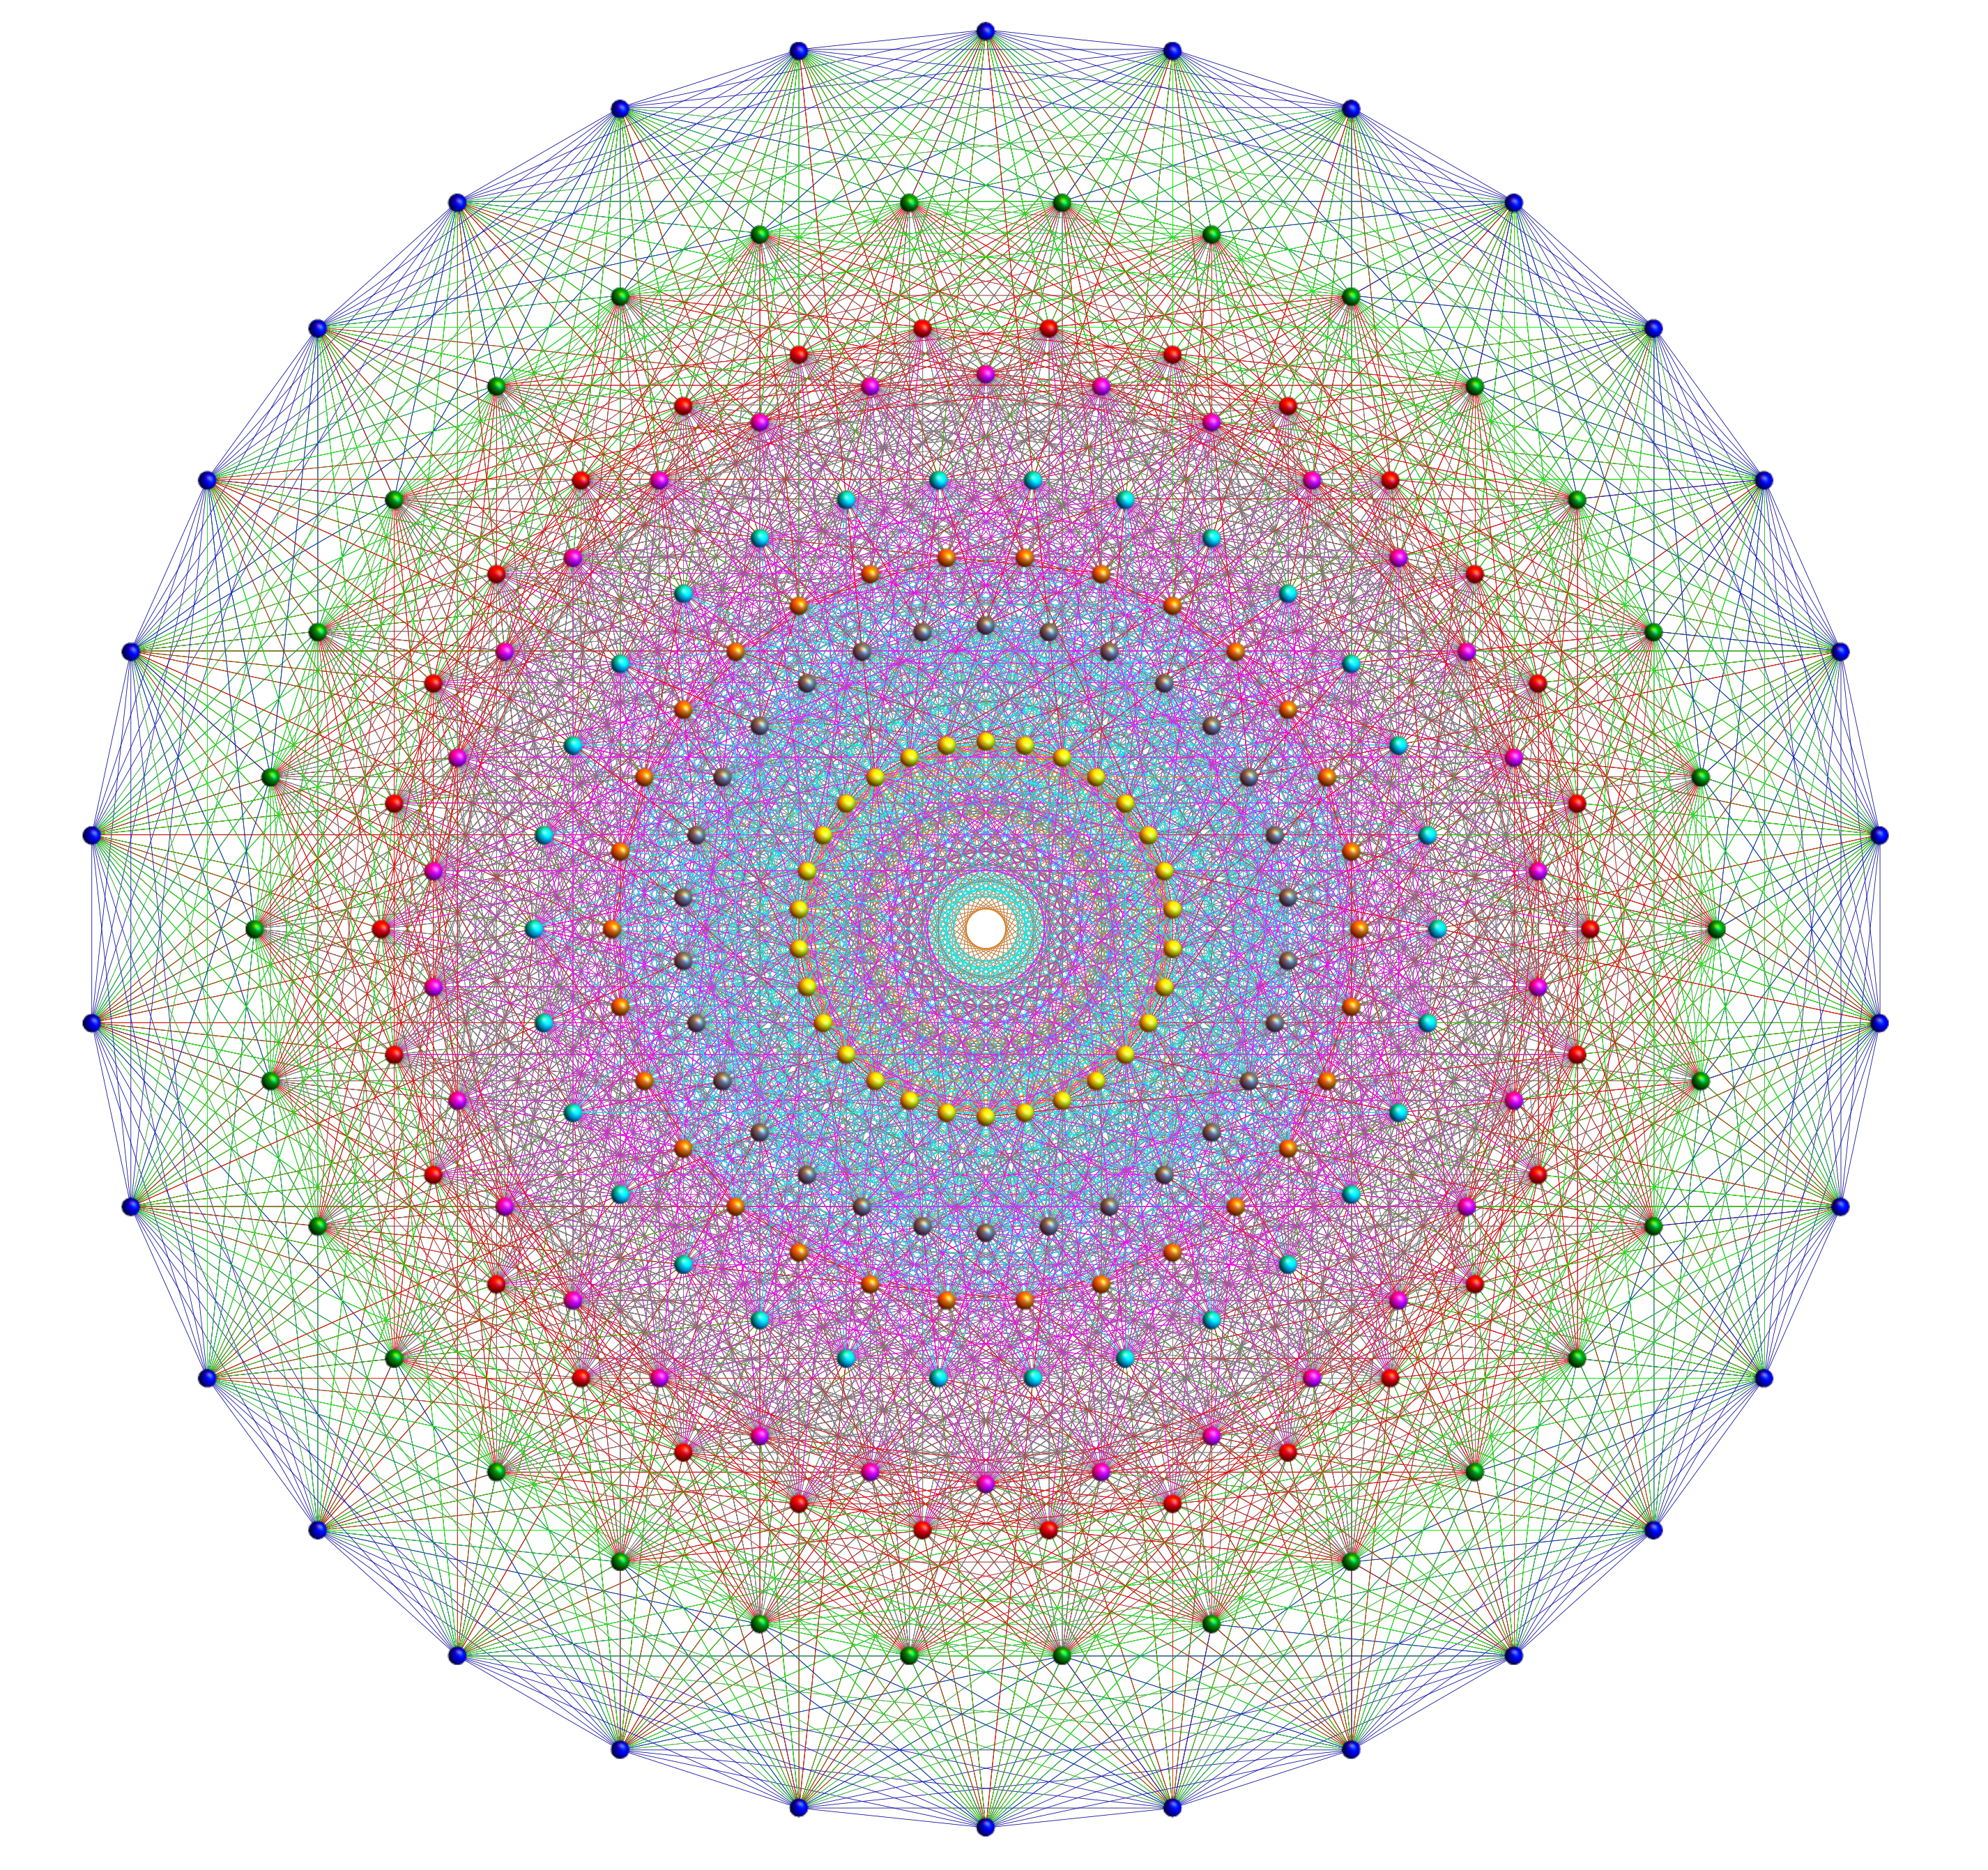
\includegraphics[width=1\columnwidth]{front.jpg}
\end{figure}
\newpage
\tableofcontents 
\newpage
\section{Struttura matematica della meccanica quantistica}
\subsection{Introduzione}
\begin{definizione}
	[Prodotto scalare]
	Per $V$ spazio vettoriale su $\mathbb{C}$ e $\psi ,\phi \in V$, si definisce $\left\langle \cdot ,\cdot  \right\rangle : V\times V \to \mathbb{C}$ come:
	\begin{itemize}
		\item $\left\langle \psi ,\phi  \right\rangle\in \mathbb{C}$;
		\item $\left\langle \psi ,\phi  \right\rangle= \left\langle \phi ,\psi  \right\rangle^*$;
		\item $\left\langle \psi, c_1\phi_1 + c_2\phi_2 \right\rangle = c_1\left\langle \psi ,\phi_1 \right\rangle + c_2 \left\langle \psi , \phi_2 \right\rangle$, con $c_1,c_2 \in \mathbb{C}$;
		\item $\left\langle \phi ,\phi  \right\rangle\ge 0$ e $\left\langle \phi ,\phi  \right\rangle=0 \iff \phi =0$.
	\end{itemize}
\end{definizione}
\noindent Dato $\phi \in V$, questo induce la \textbf{norma}:
\begin{equation}
	\left\lVert \phi  \right\rVert \overset{\text{def}}{=} \sqrt{\left\langle \phi ,\phi  \right\rangle} 
\end{equation}
Si ricordano le seguenti disuguaglianze:
\begin{equation}
	\begin{split}
		&\text{\textbf{Schwarz}: } \left\lvert \left\langle \phi ,\psi  \right\rangle \right\rvert ^2 \le  \left\langle \phi ,\phi  \right\rangle\left\langle \psi ,\psi  \right\rangle\\
		&\text{\textbf{Triangolare}: } \left\lVert \phi + \psi  \right\rVert \le  \left\lVert \psi  \right\rVert +\left\lVert \phi  \right\rVert 
	\end{split}
\end{equation}
\begin{teorema}
	[Teorema di Riesz]
	Dato $T$ operatore lineare limitato agente su spazio di Hilbert $\mathcal{H}$, allora $\exists f \in \mathcal{H}:\forall \phi \in \mathcal{H}\Rightarrow T(\phi )\equiv \left\langle f,\phi  \right\rangle$. Inoltre, $\left\lVert T \right\rVert = \left\lVert f \right\rVert $.
\end{teorema}
\begin{osservazione}
	[Funzionali e operatori]
	Un funzionale lineare \`e un operatore lineare $F$ che agisce su uno spazio vettoriale $V$ su $\mathbb{K}$ e restituisce un valore nel campo; formalmente: $F:V\to \mathbb{K}$. In generale, gli operatori non restituiscono valori in $\mathbb{K}$, mentre i funzionali s\`i.	

Gli operatori rappresentano gli osservabili, mentre i funzionali sono usati per calcolare aspettazione e probabilit\`a.
\end{osservazione}
\subsubsection{Notazione bra-ket}
Sia $V$ uno spazio vettoriale e $V'$ il suo duale; si definiscono:
\begin{itemize}
	\item per $\phi \in V \longrightarrow \ket{\phi } \in V$;
	\item per $F \in  V' \longrightarrow \bra{F} \in V'$.
\end{itemize}
Per Riesz, per qualche $f \in V$:
\begin{equation}
	\braket{F|\phi } \overset{\text{def}}{=}F(\phi ) = \left\langle f,\phi  \right\rangle \Rightarrow F(\phi ) \leftrightarrow \braket{f|\phi}
\end{equation}
Visto che $\braket{\phi |\psi } = \left\langle \phi ,\psi  \right\rangle$, allora: 
\begin{equation}
	\bra{c\phi } = c^* \bra{\phi } \longleftrightarrow \ket{c\phi } = c \ket{\phi } 
\end{equation}
\subsubsection{Operatori}
Si considerano vettori, o \textbf{stati}, in uno spazio di Hilbert $\mathcal{H}$. Un operatore che agisce su tale spazio \`e definito come $\hat{A}: \mathcal{H}\to \mathcal{H}$, quindi $\hat{A}\ket{\phi } \in \mathcal{H}$. Gli operatori di interesse saranno \textbf{lineari}.

Se $\hat{A}$ \`e limitato (quindi continuo), dato $\ket{\psi } \in \mathcal{H}$, con $\left\{ \phi _i \right\} $ base ortonormale:
\begin{equation*}
	\begin{cases}
		 \hat{A}\ket{\psi } = \ket{\phi } = \sum_{i=1}^{+\infty} c_i \ket{\phi _i}  \\
		\\
		 \hat{A}\ket{\psi } = \sum_{i=1}^{+\infty} b_i \hat{A}\ket{\phi _i} 
	\end{cases}
\end{equation*}
si nota che
\begin{equation}
	\braket{\phi _j|\hat{A}\psi } =\bra{\phi _j} \left(\sum_{i=1}^{+\infty} b_i \hat{A} \ket{\phi _i} \right)  = \sum_{i=1}^{+\infty} b_i\underbracket{\braket{\phi _j|\hat{A}|\phi _i}}_{\equiv A_{ji} } 
\end{equation}
dove $A_{ji} $ \`e un elemento di matrice; infatti
\begin{equation*}
		 \braket{\phi _j|\phi } = \braket{\phi _j|\hat{A}|\psi } = \sum_{i=1}^{+\infty}c_i \braket{\phi _j|\phi _i} = c_j
\end{equation*}
da cui, unendo le uguaglianze:
\begin{equation*}
\sum_{i=1}^{+\infty} A_{ji} b_i = c_j	
\end{equation*}
Sia $\hat{A}$ lineare; l'aggiunto \`e $\hat{A}^\dagger $ e tale che $\langle \phi , \hat{A}\psi  \rangle= \langle \hat{A}^\dagger \phi ,\psi  \rangle$. Allora, in notazione bra-ket:
\begin{equation}
	\bra{w} = \bra{\phi } \hat{A}^\dagger \longleftrightarrow \ket{w} = \hat{A}\ket{\phi } 
\end{equation}
Inoltre 
\begin{boxenv}[]
\begin{equation}
	\begin{split}
		&\left\langle \psi ,\phi  \right\rangle^* = \left\langle \phi ,\psi  \right\rangle \implies \braket{\psi |\phi } ^* = \braket{\phi |\psi }\\
		& \Rightarrow \braket{\psi  |\hat{A}^\dagger |\phi } ^* = \braket{\phi |\hat{A}|\psi } 
	\end{split}
\end{equation}
\end{boxenv}
\noindent Infine, se $\left\{ \phi _i \right\} $ base ortonormale:
\begin{boxenv}[]
\begin{equation}
	A^\dagger _{ij} = \braket{\phi _i|\hat{A}^\dagger |\phi _j} = \braket{\phi _j|\hat{A}|\phi _i} ^* = A_{ji} ^* \Rightarrow A^\dagger = (A^\top)^*
\end{equation}
\end{boxenv}
\noindent Da questo, segue:
\begin{equation}
	(AB)^\dagger = B^\dagger A^\dagger; \ (cA)^\dagger = c^* A^\dagger 
\end{equation}
\subsubsection{Operatori autoaggiunti}
\begin{definizione}
	[Operatore autoaggiunto]
	Sia \( \mathcal{H} \) uno spazio di Hilbert complesso e sia \( A \) un operatore lineare definito su un dominio \( \operatorname{Dom} (A) \subseteq \mathcal{H} \). L'operatore \( A \) si dice \textbf{autoaggiunto} se soddisfa le seguenti condizioni:

\begin{enumerate}
    \item \textbf{Densità del dominio:} il dominio \( \text{Dom}(A) \) è denso nello spazio di Hilbert \( \mathcal{H} \), ovvero:
    \[
    \overline{\text{Dom}(A)} = \mathcal{H}.
    \]

    \item \textbf{Simmetria:} per ogni \( \psi, \phi \in \text{Dom}(A) \),
    \[
    \langle \psi, A \phi \rangle = \langle A \psi, \phi \rangle.
    \]

    \item \textbf{Uguaglianza con l'aggiunto:} il dominio di \( A \) coincide con quello del suo aggiunto \( A^\dagger \), e i due operatori coincidono, ovvero:
    \[
    \text{Dom}(A) = \text{Dom}(A^\dagger) \quad \text{e} \quad A = A^\dagger.
    \]
\end{enumerate}
\end{definizione}
\noindent Essendo $\hat{A}= \hat{A}^\dagger $, si ha $A_{ij} = (A_{ij} ^*)^\top$. Questi sono sempre diagonalizzabili, quindi hanno base ortonormale di autovettori. Visto che $\braket{\phi _1|\hat{A}|\phi _2} = \braket{\phi _2|\hat{A}|\phi _1} ^*$, allora $\braket{\psi |\hat{A}|\psi } \in \mathbb{R}$ ed \`e il \textbf{valore di aspettazione}.

Sia $\ket{\psi } $ autostato di $\hat{A}$ autoaggiunto; allora $\hat{A} \ket{\psi } = a \ket{\psi } \Rightarrow \bra{\psi } \hat{A}=  \bra{\psi } a^*$. Si nota, per\`o, che:
\begin{equation}
	a \braket{\psi |\psi } = \braket{\psi |\hat{A}|\psi } = \braket{\psi |\hat{A}^\dagger |\psi } = a^* \braket{\psi |\psi } \iff a=a^* \Rightarrow a \in \mathbb{R}
\end{equation}
Siano $\ket{\psi_1} , \ket{\psi_2} $ tali che $\hat{A}\ket{\psi_1} = a_1 \ket{\psi_1} $ e $\hat{A}\ket{\psi_2} = a_2\ket{\psi_2} $, con $a_1\neq a_2$; allora:
\begin{equation}
	\begin{split}
		& a_2 \braket{\psi_1|\psi_2} = \braket{\psi_1|\hat{A}|\psi_2} = \braket{\psi_1|\hat{A}^\dagger |\psi_2} = a_1^* \braket{\psi_1|\psi_2}= a_1 \braket{\psi_1|\psi_2} \\
		&\Rightarrow (a_2-a_1) \braket{\psi_1|\psi_2}=0 \iff \ket{\psi_1} \perp \ket{\psi_2} 
	\end{split}
\end{equation}
\subsubsection{Commutatori}
\begin{definizione}
	[Commutatore]
	Siano $\hat{A},\hat{B}$ due operatori; il commutatore \`e: $[ \hat{A},\hat{B} ] \overset{\text{def}}{=} \hat{A}\hat{B} - \hat{B}\hat{A}$. Quindi se $\hat{A},\hat{B}$ commutano, si ha $[ \hat{A},\hat{B} ] =0$.
\end{definizione}
\begin{teorema}
	[Spettro comune]
	Se $\hat{A},\hat{B}$ sono autoaggiunti e commutano, allora condividono una base di autovettori.
\end{teorema}
\subsection{Prodotto esterno}
Applicazione $\rho : V \times  V \to \mathcal{O}$, con $\mathcal{O}$ spazio degli operatori lineari. Un esempio di prodotto esterno \`e l'operatore lineare
\begin{boxenv}[]
\begin{equation}
	\hat{O} = \ket{\psi } \bra{\phi } : V \to V
\end{equation}
\end{boxenv}
\noindent Si nota che:
\[
\begin{split}
	&\braket{v|\hat{O}w} = \braket{v|(\ket{\psi } \bra{\phi } ) w} = \braket{v|\psi } \braket{\phi |w}=\braket{ \hat{O}^\dagger v|w} \iff O^\dagger = \ket{\phi}\bra{\psi  }  
\end{split}
\] 
\subsubsection{Proiettori}

Operatore $\hat{P}$ tale che $\hat{P}^2 = \hat{P}$. Un esempio \`e $\hat{P}=\ket{\psi } \bra{\psi } $, con $\left\lVert \psi  \right\rVert =1$ perch\'e:
\[
\hat{P}^2 = \ket{\psi } \braket{\psi |\psi } \bra{\psi } =\ket{\psi } \bra{\psi } \equiv \hat{P}
\] 
\subsubsection{Completezza di una base e valore di aspettazione di un osservabile}

Un insieme ortonormale $\left\{ \ket{\phi_i }  \right\} $ si dice completo se:
\begin{boxenv}[]
\begin{equation}
	\sum_{i=1}^{+\infty} \ket{\phi _i} \bra{\phi _i} = \operatorname{Id} 
\end{equation}
\end{boxenv}
\noindent Un insieme ortonormale completo \`e una base ortonormale di $\mathcal{H}$, quindi permette di scomporre ogni stato in una combinazione lineare.
\subsubsection{Cambiamento di base}
Siano $\left\{ \ket{\phi _i}  \right\}_i , \ \left\{ \ket{\psi _i}  \right\}_i $ basi ortonormali. Si esprime una in funzione dell'altra:
\begin{equation}
	\ket{\psi _i} = \left(\sum_{j=1}^{+\infty} \ket{\phi _j} \bra{\phi _j} \right) \ket{\psi _i} = \sum_{j=1}^{+\infty} \braket{\phi _j|\psi _i} \ket{\phi _j} \equiv \sum_{j=1}^{+\infty} S^* _{ij} \ket{\phi _j} 
\end{equation}
Per $\varphi $ generico stato: $\ket{\varphi } = \sum_{i=1}^{+\infty} a_i \ket{\phi _i} = \sum_{i=1}^{+\infty} b_i \ket{\psi _i} $; allora:
\begin{equation}
	\begin{cases}
		\displaystyle b_i=\braket{\psi _i|\varphi } = \sum_{j=1}^{+\infty} a_j \braket{\psi _i|\phi _j} \equiv \sum_{j=1}^{+\infty} S_{ij} a_j\\
		\\
		\displaystyle a_i = \braket{\phi _i|\varphi } =\sum_{j=1}^{+\infty} b_j \braket{\phi _i|\psi _j} \equiv \sum_{j=1}^{+\infty} S_{ji}^* b_j
	\end{cases}
\end{equation}
Ora, essendo le due basi ortonormali:
\begin{equation}
	\delta _{ij} = \Braket{\phi _i|\left(\sum_{k=1}^{+\infty} \left\lvert \psi _k \right\rangle\left\langle \psi _k \right\rvert \right) \phi _j} = \sum_{k=1}^{+\infty} \braket{\phi _i|\psi _k} \braket{\psi _k|\phi _j} = \sum_{k=1}^{+\infty} S_{ki} ^* S_{kj} 
\end{equation}
da cui $S^\dagger S = \operatorname{Id} $.

\subsection{Applicazioni per la meccanica quantistica}

\subsubsection{Rappresentazione delle coordinate}
Uno stato si decompone in maniera diversa a seconda della base; ogni decomposizione \`e una sua diversa \textbf{rappresentazione}. 

Sia $\hat{Q}:\mathcal{H}\to \mathcal{H}$ operatore autoaggiunto \textbf{posizione}\footnote{Indicato anche con $\hat{X}$.}, con $\hat{Q}\ket{x} =x \ket{x} $\footnote{Gli autostati sono le $x$, mentre $\ket{x} $ rappresenta gli autovettori.}. Il suo spettro \`e continuo, quindi la decomposizione spettrale avviene tramite integrale: dato uno stato $\ket{\psi }\in \mathcal{H}$
\begin{equation}
	\ket{\psi } = \int_{-\infty} ^{+\infty} \braket{x|\psi } \ket{x } \ dx \equiv \int_{-\infty} ^{+\infty} \psi (x) \ket{x} \ dx 
\end{equation}
con $\psi (x)$ \textbf{funzione d'onda} dello stato $\ket{\psi } $ e ne indica i coefficienti nella rappresentazione delle coordinate.
\subsubsection{Rappresentazione degli impulsi}
Sia $\hat{p}\ket{p} = p \ket{p} $ operatore impulso (autoaggiunto); per $\ket{\psi } \in \mathcal{H}$:
\begin{equation}
	\ket{\psi } = \int_{-\infty} ^{+\infty} dp \ c(p) \ket{p} \equiv \int_{-\infty} ^{+\infty} dp \ \widetilde{\psi }(p) \ket{p} 
\end{equation}
dove $\widetilde{\psi }(p) $ \`e la funzione d'onda nel dominio degli impulsi e si ottiene trasformando con Fourier $\psi (x)$.
\subsubsection{Misura di un osservabile}
Sia $\hat{A}$ operatore lineare autoaggiunto\footnote{In generale, ogni operatore in meccanica quantistica, almeno quelli associati ad osservabili, sono operatori lineari autoaggiunti.} con autovalori $a_i$ e autovettori $\ket{\lambda _i} $. Assumendo che $\braket{\lambda _i|\lambda _j} = \delta _{ij} $ formino una base ortonormale\footnote{Possono essere sempre costruiti in modo che siano ortonormali.} e dato un generico $\ket{\psi } = \sum_{i=1}^{+\infty}b_i \ket{\lambda _i} $, si nota che :
\begin{equation}
	\braket{\psi |\hat{A}|\psi } = \left[ \sum_{i=1}^{+\infty} b^*_j \bra{\lambda _i}  \right] \left[ \sum_{j=1}^{+\infty} b_j \hat{A}\ket{\lambda _j}  \right]= \sum_{i=1}^{+\infty} \left\lvert b_i \right\rvert ^2 a_i
\end{equation}
\noindent dove si pu\`o vedere $\left\lvert b_i \right\rvert ^2$ come probabilit\`a di ottenere misura $a_i$ da osservabile $\hat{A}$. In questo senso, deve valere:
\[
\sum_{i=1}^{+\infty} \left\lvert b_i \right\rvert ^2 \stackrel{!}{=}1
\] 
Questa condizione \`e verificata dalla normalizzazione di ciascuno stato:
\begin{equation}
		\braket{\psi |\psi } = \left[ \sum_{i=1}^{+\infty} b_i^* \bra{\lambda _i}  \right] \left[ \sum_{j=1}^{+\infty} b_j \ket{\lambda _j}  \right] = \sum_{i,j=1}^{+\infty} b_i^* b_j \braket{\lambda _i|\lambda _j} =\sum_{i=1}^{+\infty} \left\lvert b_i \right\rvert ^2 \stackrel{!}{=}1
\end{equation}
\noindent Per un operatore a spettro continuo $\hat{F}$, con autovettori $\ket{z} $ relativi ad autovalori $z$ e $\ket{\psi } \in \mathcal{H}, \  \ket{\psi } = \int_{-\infty} ^{+\infty} f(z) \ket{z} \ dz, \ f(z) = \braket{z|\psi }$:
\begin{equation}
	\begin{split}
		&\begin{split}
			\braket{\psi| \hat{F}|\psi }&=\int_{-\infty} ^{+\infty} f^*(y) \bra{y}\ dy \int_{-\infty} ^{+\infty} f(z) \hat{F}\ket{z} \ dz\\
						    &= \int_{-\infty} ^{+\infty} \int_{-\infty} ^{+\infty} dydz \ f^*(y) f(z) z\braket{y|z} = \int_{-\infty} ^{+\infty} z\left\lvert f(z) \right\rvert ^2 \ dz
		\end{split}\\
		&\braket{\psi |\psi } = \int_{-\infty} ^{+\infty} \left\lvert f(z) \right\rvert ^2 \ dz \stackrel{!}{=}1 \text{ \textbf{(normalizzazione)} }
	\end{split}
\end{equation}
\subsubsection{Principi della meccanica quantistica}
\begin{enumerate}[(a).]
	\item Uno stato fisico $\ket{\psi } $ \`e un vettore in uno spazio di Hilbert $\mathcal{H}$, $\ell ^2$ o $L^2$. Lo stesso stato pu\`o essere equivalentemente moltiplicato per una fase: $e^{i\alpha } \ket{\psi } $.
	\item Per ogni sistema, ogni stato deve essere tale che $\braket{\psi |\psi } =1$.
	\item Gli osservabili sono operatori lineari autoaggiunti che agiscono su $\mathcal{H}$.
	\item Il valore di aspettazione di un osservabile $\hat{A}$ relativo ad uno stato $\ket{\psi } $ \`e $\braket{\psi |\hat{A}|\psi } $. Se $a_i$ sono autovalori, con $\ket{a_i} $ relativi autovettori, di $\hat{A}$, la probabilit\`a di ottenere la misura $a_i$ (data dal fatto che il sistema \`e nello stato $\ket{a_i} $) \`e $\left\lvert a_i \right\rvert ^2$. 

		Nel caso di operatori con spettri continui, si costruisce la densit\`a di probabilit\`a $P(x) dx = \left\lvert \psi (x) \right\rvert ^2 dx$ (come esempio per operatore posizione $\hat{Q}$) ed \`e probabilit\`a di trovare la particella nell'intervallo spaziale $dx$.
\end{enumerate}
\subsubsection{Spazio di Hilbert proiettivo, sistemi puri e misti}
Ogni stato $\ket{\psi } $ \`e definito a meno di una fase; per eliminare fase globale, si usa lo spazio proiettivo $\mathcal{P}(\mathcal{H}) = \mathcal{H} /\mathord{\sim}$, con $\ket{\psi } \sim e^{i\alpha }  \ket{\psi } $.

Con gli elementi di $\mathcal{P}(\mathcal{H})$ si pu\`o introdurre un \textbf{isomorfismo naturale}\footnote{Isomorfismo che non dipende dalla scelta del rappresentante della classe di equivalenza.} con lo spazio generato dagli operatori $\rho = \ket{\psi } \bra{\psi } $, nel caso di sistemi \textbf{puri}. 

Un sistema quantistico puro, \`e univocamente descritto da un singolo stato $\ket{\psi } $ (quello in cui si trova in un certo istante temporale), quindi il proiettore $\rho  = \ket{\psi } \bra{\psi } $ contiene tutte le informazioni necessarie per una sua descrizione. Un sistema \textbf{misto}, invece, non pu\`o essere descritto tramite un singolo stato perch\'e appartiene a pi\`u stati puri contemporaneamente in una certa proporzione; in questo caso, il proiettore diventa una \textbf{matrice di densit\`a}  con 
\begin{equation}
	\rho = \sum_{i} p_i \ket{\psi _i} \bra{\psi _i} 
\end{equation}
\subsubsection{Proiettore per sistemi puri}
La condizione di normalizzazione \`e:
\begin{equation}
	\operatorname{Tr} \rho = 1
\end{equation}
\begin{boxenv}[]
\begin{proof}
	Se $\ket{\psi } = \sum_{n=1}^{+\infty} c_n \ket{\phi _n} $:
	\begin{equation}
		\begin{split}
			\operatorname{Tr} \rho  &\overset{\text{def}}{=} \sum_{m=1}^{+\infty} \sum_{n=1}^{+\infty} \braket{\phi _m|\rho |\phi _n} \delta _{mn} = \sum_{n=1}^{+\infty} \braket{\phi _n|\rho |\phi _n}  = \sum_{n=1}^{+\infty} \braket{\phi _n|\psi } \braket{\psi |\phi _n} \\
			&=\sum_{n=1}^{+\infty} \left\lvert \braket{\phi _n|\psi }  \right\rvert ^2 = \braket{\psi |\psi }  		\end{split}
	\end{equation}
	dove l'ultima uguaglianza deriva dalla completezza di $\left\{ \ket{\phi _n}  \right\}_n $.
\end{proof}
\end{boxenv}
\noindent Un generico elemento di matrice di $\rho = \ket{\psi } \bra{\psi } $ \`e $\rho _{ij} = c_i c_j^*$, dove $\ket{\psi } = \sum_{i}^{} c_i \ket{\phi _i} $.
\begin{boxenv}
\begin{proof}
	Per conto diretto:
	\begin{equation}
		\begin{split}
			\rho _{ij} &= \braket{\phi _i|\rho |\phi _j} = \braket{\phi _i|\psi } \braket{\psi |\phi _j} = \sum_{m=1}^{+\infty} c_m \braket{\phi _i|\phi _m} \sum_{n=1}^{+\infty} c_n^* \braket{\phi _n|\phi _j} \\
			&=\sum_{m,n=1}^{+\infty} c_m c_n^* \delta _{im} \delta _{jn} = c_ic_j^*
		\end{split}
	\end{equation}
\end{proof}
\end{boxenv}
\noindent Dato $\hat{A}$ osservabile con base di autostati $\left\{ \ket{a_i}  \right\} _i$:
\begin{equation}
	\braket{\psi |\hat{A}|\psi } = \operatorname{Tr} \rho \hat{A}
\end{equation}
\begin{boxenv}[]
\begin{proof}
	Si prende $\psi = \sum_{i}^{} c_i \ket{a _i} $ e $\rho = \ket{\psi } \bra{\psi }  $; allora: 
	\begin{equation}
			\operatorname{Tr} (\rho \hat{A}) \overset{\text{def}}{=} \sum_{i}^{} \braket{a _i|\rho \hat{A}|a _i} = \sum_{i}^{} a_i \braket{a_i|\rho |a_i} = \sum_{i}^{} \lvert c_i \rvert ^2 a_i \equiv \braket{\psi |\hat{A}|\psi } 
	\end{equation}
\end{proof}
\end{boxenv}
\subsubsection{Flusso di probabilit\`a ed equazione di continuit\`a}\label{fp}

Sistema composto da particella in 3D sotto potenziale $V(x)$. Sia $\psi (\mathbf{x} ,t)$ funzione d'onda per stato $\ket{\psi(t) } $. La probabilit\`a di trovare particella in una regione $\Gamma$ dello spazio \`e\footnote{I termini con il potenziale si cancellano perch\'e simmetrici, mentre quelli con $\nabla ^2$ no perch\'e in uno sar\`a derivato $\psi $, nell'altro $\psi ^*$.}:
\begin{equation}
	P_\Gamma (t) \equiv\int_{\Gamma} d^3 x \ \lvert \psi (\mathbf{x} ,t) \rvert ^2 
\end{equation}
Per quanto detto in \S\ref{pice}: $i\hbar  \partial _t \psi (\mathbf{x} ,t) = \left(- \frac{\hbar ^2}{2m} \nabla ^2 + V(\mathbf{x} )\right) \psi (\mathbf{x} ,t)$; evoluzione temporale di $P_\Gamma(t)$ \`e:
\[
\begin{split}
	\partial _t P_\Gamma(t) &= \partial _t \int_{\Gamma}d^3 x \ \psi (\mathbf{x} ,t) \psi ^*(\mathbf{x} ,t) = \int_{\Gamma} \big[\psi ^*(\mathbf{x} ,t) \partial _t \psi (\mathbf{x} ,t) + \psi (\mathbf{x} ,t) \partial _t \psi ^*(\mathbf{x} ,t)\big] \ d^3x \\
				& = \int_{\Gamma} \left[ \psi ^*(\mathbf{x} ,t) \frac{1}{i\hbar } \left(- \frac{\hbar ^2}{2m} \nabla ^2 + V(x) \right) \psi (\mathbf{x} ,t) - \frac{1}{i\hbar } \left(- \frac{\hbar ^2}{2m} \nabla ^2 + V(x) \right) \psi^* (\mathbf{x} ,t)  \right]  \ d^3x \\
				&= \frac{i\hbar }{2m}\int_{\Gamma} \big[\psi ^*(\mathbf{x} ,t) \nabla ^2 \psi (\mathbf{x} ,t) - \psi (\mathbf{x},t) \nabla ^2 \psi ^*(\mathbf{x} ,t) \big]	\ d^3x= \frac{i\hbar }{2m} \int_{\Gamma} \nabla \cdot \big(\psi ^* \nabla \psi - \psi \nabla \psi ^*\big)	\ d^3x
\end{split}
\] 
Definendo \textbf{flusso di probabilit\`a}:
\begin{boxenv}[]
\begin{equation}
	\mathbf{J} = - \frac{i\hbar }{2m} \big( \psi ^* \nabla \psi  - \psi \nabla \psi ^*\big)
\end{equation}
\end{boxenv}
\noindent si ha:
\begin{equation}
	\partial _t P_\Gamma(t) = - \int_{\Gamma} \nabla \cdot \mathbf{J} \ d^3 x 
\end{equation}
da cui si ottiene equazione di continuit\`a:
\begin{boxenv}[]
\begin{equation}
	\partial _t \lvert \psi  \rvert ^2 + \nabla \cdot \mathbf{J} =0
\end{equation}
\end{boxenv}

\newpage	
\section{Introduzione alla meccanica quantistica}
\subsection{Evoluzione temporale}
\subsubsection{Equazione di Shr\"odinger per gli stati}

Variazione temporale dello stato di un sistema: $\ket{\psi (t)} $ o $\ket{\psi ,t} $. Per la funzione d'onda: $\psi (x,t) = \braket{x|\psi (t)} $. Per trovare evoluzione temporale di uno stato, si richiede che:
\begin{enumerate}[(a).]
	\item l'evoluzione sia univocamente determinata da uno stato iniziale $\Rightarrow $ si richiede che nell'equazione compaia al massimo il primo ordine di derivazione $\partial _t\ket{\psi (t)}$;
	\item sperimentalmente, si verifica il principio di sovrapposizione, quindi l'equazione differenziale deve essere lineare.
\end{enumerate}
L'equazione risultante \`e:
\begin{equation}
	i \hbar \partial _t \ket{\psi (t)} = \hat{H}\ket{\psi (t)} 
\end{equation}
$\hat{H}$ \`e un generico operatore che definisce l'evoluzione temporale del sistema. Deve risultare autoaggiunto.
\begin{boxenv}[]
\begin{proof}
	Da $\braket{\psi (t)|\psi (t)} \stackrel{!}{=}1, \ \forall t$:
	\begin{equation}
		\begin{split}
			&0\stackrel{!}{=} \partial _t \braket{\psi (t)|\psi (t)} = \big(\partial _t \bra{\psi (t)} \big)\ket{\psi (t)}  + \bra{\psi (t)} \big(\partial _t\ket{\psi (t)} \big)\\
			&\Rightarrow \frac{i}{\hbar} \braket{\psi (t)|\hat{H}^\dagger |\psi (t)} = \frac{i}{\hbar} \braket{\psi (t)|\hat{H}|\psi (t)} \Rightarrow \hat{H}^\dagger = \hat{H}
		\end{split}
	\end{equation}
\end{proof}
\end{boxenv}
\noindent Questo candida $\hat{H}$ come osservabile
\subsubsection{Soluzione dell'equazione}

La soluzione \`e:
\begin{equation}
	\ket{\psi (t)} = e^{-\frac{i}{\hbar } \hat{H}(t-t_0) } \ket{\psi (t_0)} 
\end{equation}
dove 
\begin{equation*}
	e^{\hat{A}} \overset{\text{def}}{=} 1+ \hat{A}+\frac{1}{2}\hat{A}^2 + \ldots
\end{equation*}
Visto che $\hat{H}$ \`e autoaggiunto, l'esponenziale \`e unitario:
\begin{equation}
e^{- \frac{i}{\hbar} \hat{H}(t-t_0)} e^{\frac{i}{\hbar } \hat{H}(t-t_0)}  = \operatorname{Id} 
\end{equation}
Definendo l'\textbf{evolutore} come l'operatore $\hat{U}(t,t_0)$ tale che $\ket{\psi (t)}  = \hat{U}(t,t_0) \ket{\psi(t_0) } $, risulta $\hat{U}(t,t_0) \hat{U}^\dagger(t,t_0) = \operatorname{Id} $. Se $\hat{H}$ \textbf{indipendente dal tempo}, allora $\hat{U}(t,t_0) = e^{- \frac{i}{\hbar}\hat{H}(t-t_0)} $.
\subsubsection{Equazione di Shr\"odinger per la funzione d'onda}
Per $\left\{ \ket{x}  \right\} $ base ortonormale $\Rightarrow \int_{-\infty} ^{+\infty} dx \ \braket{\psi (t)|x} \braket{x|\psi (t)} =\int_{-\infty}^{+\infty}   dx \ \left\lvert \psi (x,t) \right\rvert ^2 \stackrel{!}{=}1$ per normalizzazione. Nell'eq. di Shr\"odinger:
\begin{equation}
	i \hbar \partial _t \ket{\psi (t)}  = \hat{H} \ket{\psi (t)} \Rightarrow  i\hbar \partial _t \braket{x|\psi (t)} = \braket{x|\hat{H}|\psi (t)} \Rightarrow i\hbar \partial _t \psi (x,t) = \hat{H}\psi (x,t)
\end{equation}
Il passaggio $ \braket{x|\hat{H}|\psi (t)} \stackrel{*}{=} \hat{H}\psi (x,t)$ \`e giustificato con l'accorgimento che gli $\hat{H}$ non sono gli stessi: uno agisce su ket, l'altro su scalare; la definizione di $\hat{H}$ agente su $\psi (x,t)$ \`e:
\[
\braket{x|\hat{H}|\psi (t)} \equiv \int_{-\infty}^{+\infty}  dy\ \braket{x|\hat{H}|y} \braket{y|\psi (t)} \overset{\text{def}}{=} \hat{H} \psi (x,t)
\] 
con $\braket{x|\hat{H}|y} $ \`e l'elemento di matrice dell'Hamiltoniano originale nella rappresentazione delle coordinate. 

Per la soluzione dell'equazione:
\[
	\begin{split}
		&\ket{\psi (t)}  = \hat{U}(t,t_0) \ket{\psi (t_0)} \Rightarrow \braket{x|\psi (t)} = \psi (x,t)= \braket{x|\hat{U}(t,t_0)|\psi (t_0)} \\
		&\Rightarrow \psi (x,t) = \int_{-\infty} ^{+\infty} dy \ \braket{x|\hat{U}(t,t_0)|y} \braket{y|\psi (t_0)} = \int_{-\infty} ^{+\infty} dy \ \hat{U}(x,y,t,t_0) \psi (y,t_0)\\
		&\Rightarrow \psi (x,t) = \hat{U}(t,t_0) \psi (x,t_0)
	\end{split}
\] 
dove, come prima, i due $\hat{U}$ non sono gli stessi.

\subsubsection{Equazione di Shr\"odinger per il proiettore}

Partendo da $\hat{\rho }(t)= \ket{\psi (t)} \bra{\psi (t)} $, si trova:
\begin{equation}
	\begin{split}
		\partial _t \hat{\rho }(t) &= \big[\partial _t \ket{\psi (t)} \big] \bra{\psi (t)} + \ket{\psi (t)} \big[\partial _t \bra{\psi (t)} \big] \\
					   &= - \frac{i}{\hbar } \hat{H} \ket{\psi (t)} \bra{\psi (t)}  + \frac{i}{\hbar } \ket{\psi (t)} \bra{\psi (t)} \hat{H}^\dagger  =-\frac{i}{\hbar }\hat{H} \hat{\rho }(t) + \frac{i}{\hbar }\hat{\rho} (t)\hat{H}\\
					   &= - \frac{i}{\hbar }\left[ \hat{H},\hat{\rho }(t) \right] 
	\end{split}
\end{equation}
\subsection{Evoluzione temporale per gli operatori}
Ci sono tre quadri per vedere il problema:
\begin{enumerate}[(a).]
	\item \textbf{quadro di Shr\"odinger:} solo gli stati dipendono dal tempo, mentre gli operatori no;
	\item \textbf{quadro di Heisenberg:} solo gli operatori dipendono dal tempo;
	\item \textbf{quadro misto (o di interazione):} l'Hamiltoniano si divide in $\hat{H} = \hat{H}_0 + \hat{H}_I$, dove il primo evolve gli operatori e il secondo evolve gli stati.
\end{enumerate}
\subsubsection{Il quadro di Shr\"odinger}
Evoluzione temporale di $\hat{O}$, con $\partial _t \hat{O}=0$, \`e: 
\begin{equation}
	\begin{split}
		\partial _t  \braket{\psi (t)|\hat{O}|\psi (t)} &= \frac{i}{\hbar }\braket{\psi (t)|\hat{H}\hat{O}|\psi (t)} - \frac{i}{\hbar }\braket{\psi (t)|\hat{O}\hat{H}|\psi (t)} \\
	&= \Braket{\psi (t)|\frac{i}{\hbar }\left[ \hat{H},\hat{O} \right] |\psi (t)} 
	\end{split}
\end{equation}
Operatore \textbf{velocit\`a} definito come $\hat{v}= \frac{i}{\hbar }\left[ \hat{H},\hat{Q} \right] $.

\subsubsection{Il quadro di Heisenberg}

Gli stati evolvono tramite operatore, quindi si definisce $\hat{O}_H (t)$ come:
\begin{equation}
	\Braket{\psi (t_0)|e^{\frac{i}{\hbar }\hat{H}t} \hat{O}e^{-\frac{i}{\hbar }\hat{H}t} |\psi (t_0)} \equiv \braket{\psi (t_0)|\hat{O}_H(t)|\psi (t_0)} 
\end{equation}
dove si nota che ancora $\hat{O}$ non dipende dal tempo.
\subsubsection{Evoluzione delle misure}

Modello della mq prevede che operatore $\hat{O}$ autoaggiunto applicato ad uno stato $\ket{\psi } $ restituisca valore rappresentato da $\hat{O}$ in tale stato. In questo senso, potendo espandere $\ket{\psi } $ in autostati di $\hat{O}$, le misure sono gli autovalori dell'operatore e, a seconda del tipo di spettro, sono continui, discreti o entrambi.

Per l'energia (quindi se $\hat{O}\equiv \hat{H}$), se $\ket{\psi _n} $ autostato dell'autovalore $E_n$: $\hat{H}\ket{\psi _n} = E_n \ket{\psi _n} $, dove $E_n$ \`e energia dello stato $\ket{\psi _n} $. 

Sia $\ket{\phi(t) }  = \exp\left(-\frac{i}{\hbar }\hat{H}(t-t_0)\right) \ket{\phi (t_0)} $ un generico stato, con $\ket{\phi (t_0)} =\sum_{n}^{} c_n \ket{\psi _n(t_0)} $. Allora:
\begin{equation}
	\ket{\phi (t)} = \sum_{n=1}^{+\infty} c_n e^{-\frac{i}{\hbar } \hat{H}(t-t_0)} \ket{\psi _n(t_0)} = \sum_{n=1}^{+\infty} c_n e^{-\frac{i}{\hbar }E_n (t-t_0)} \ket{\psi _n(t_0)}  
\end{equation}
L'esponenziale \`e una fase, quindi $\ket{\phi (t)} $ \`e \textbf{stazionario}. Per questo, se $\hat{O}$ operatore: $\braket{\psi _n(t)|\hat{O}|\psi _n(t)} = \braket{\psi _n(t_0)|\hat{O}|\psi _n(t_0)} $, da cui $E_n(t) = E_n(0)$ per $\hat{O}\equiv \hat{H}$.


\subsection{Simmetrie e operatore impulso}
\subsubsection{Traslazioni}

Sia trasla $\ket{\psi } \to \ket{\psi '} $, $\hat{A}\to \hat{A}'$, e, assumendo simmetria per traslazioni spaziali, si richiede che per $\hat{A}\ket{\phi _n} =a_n\ket{\phi _n} \to \hat{A}' \ket{\phi _n} = a'_n \ket{\phi '_n}  $ si abbia $a'_n = a_n$. Se $\ket{\psi } = \sum_{n}^{} c_n \ket{\phi _n} $ e $\ket{\psi '} = \sum_{n}^{} c'_n\ket{\phi '_n} $, deve valere $\left\lvert c_n \right\rvert ^2 = \left\lvert c'_n \right\rvert ^2$ perch\'e sonno le probabilit\`a di ottenere una certa misura. L'invarianza per traslazione \`e assicurata quando:
\begin{equation}
	\begin{cases}
		a'_n = a_n\\
		\left\lvert c'_n \right\rvert ^2 = \left\lvert c_n \right\rvert ^2
	\end{cases}
\end{equation}
Si cerca $\hat{U}$ operatore delle traslazioni. Si assume che questo soddisfi:
\begin{equation}
\begin{cases}
\ket{\psi '} = \hat{U}\ket{\psi }, \ \forall \ket{\psi } \in \mathcal{H}\\
\braket{\phi '|\psi '} = \braket{\phi |\psi } , \ \forall \ket{\phi } , \ket{\psi } \in \mathcal{H} 
\end{cases}
\end{equation}
Unendo le due, si trova $\hat{U}$ unitario:
\begin{equation}
	\braket{\phi '|\psi '} = \braket{\phi |\hat{U}^\dagger \hat{U}|\psi } \Rightarrow \hat{U}^\dagger \hat{U}= \operatorname{Id} 
\end{equation}
Su generico operatore $\hat{A}$ come sopra:
\begin{equation}
	\begin{split}
		&\hat{A}' \hat{U}\ket{\phi _n} = a_n \hat{U}\ket{\phi _n} = \hat{U}a_n \ket{\phi _n} = \hat{U}\hat{A}\ket{\phi _n} \Rightarrow \hat{A'}\hat{U}\ket{\phi _n} = \hat{U}\hat{A}\ket{\phi _n} \\
		&\Rightarrow \hat{A}' = \hat{U}\hat{A}\hat{U}^\dagger 
	\end{split}
\end{equation}
Si definisce azione di $\hat{U}$ su una funzione d'onda:
\begin{equation}
	\psi '(x) = \braket{x|\psi '} = \braket{x|\hat{U}|\psi } \overset{\text{def}}{=}\hat{U} \psi (x)\Rightarrow \psi '(x) = \hat{U}\psi (x) 
\end{equation}
\subsubsection{L'operatore impulso}
Visto $\hat{U}$ unitario, si prende $\hat{U} (s) = e^{is \hat{K}} $ per parametrizzare la traslazione con parametro continuo $s$. Si mostra che $\hat{K}$ \`e autoaggiunto\footnote{Quindi sar\`a un possibile osservabile.}. Sviluppando attorno a $s=0$: 
\begin{equation}
	\hat{U}(s) \simeq \hat{U}(0) + \Eval{s \frac{d }{d s} \hat{U}(s) }{s=0}{} + \operatorname{O} (s^2) = \operatorname{Id} + is \hat{K} + \operatorname{O} (s^2)
\end{equation}
Dovendo essere $\hat{U}(s) \hat{U}^\dagger (s) =\operatorname{Id} $, trascurando $\operatorname{O} (s^2)$:
\begin{equation}
	\left(\operatorname{Id}+ s \frac{d }{d s} \hat{U}^\dagger (s)\right) \left(\operatorname{Id} + s\frac{d }{d s}\hat{U}(s) \right) = \left(\operatorname{Id} - is \hat{K}^\dagger \right) \left(\operatorname{Id} + is\hat{K}\right)\simeq \operatorname{Id} + is (\hat{K}-\hat{K}^\dagger )
\end{equation}
da cui $\hat{K}=\hat{K}^\dagger $. 

Si introduce operatore \textbf{impulso}\footnote{Questa introduzione \`e giustificata dal fatto che, per il teorema di N\"other, l'impulso \`e il generatore delle traslazioni spaziali.} come $\hat{K}= - \frac{1}{\hbar } \hat{p}$, da cui $\hat{U}(s) = \exp\left(-\frac{i}{\hbar }s \hat{p}\right) $. Si ricava la sua rappresentazione nello spazio delle posizioni. Sviluppando\footnote{Si ottiene l'espressione di $\hat{p}$ nella rappresentazione delle coordinate sotto l'assunzione che una traslazione abbia il seguente effetto su una funzione d'onda: $\psi '(x) \equiv \hat{U}\psi (x) = \psi (x-s)$.}:
\begin{equation}
	\begin{split}
		&\hat{U}\psi (x) \simeq \left(1- \frac{i}{\hbar }s \hat{p}\right) \psi (x)\\
		& \psi'(x) \equiv \psi (x-s) \simeq \psi (x) + s \Eval{\frac{d }{d s} \psi (x-s)}{s=0}{} = \psi (x) - s \partial _x \psi (x)\\
		&\Rightarrow \left(1-\frac{i}{\hbar }s \hat{p}\right) \psi (x) = \psi (x) - s \partial _x \psi (x)
	\end{split} 
\end{equation}
Da cui $\hat{p}= - i \hbar \partial _x$. 

\subsubsection{Funzione d'onda degli impulsi}

Visto che $\hat{p}\ket{\psi } = -i\hbar \partial _x\ket{\psi } $, vale $\braket{x|\hat{p}|p} = \hat{p}\braket{x|p}  \equiv \hat{p} \psi _p(x)\Rightarrow -i \hbar  \partial _x \psi _p(x) = p \psi _p(x)$, quindi $\psi _p(x) = \braket{x|p} = C \exp\left(\frac{i}{\hbar }p x\right) $. Per $C$, si usa normalizzazione:
\[
\delta (p'-p) = \braket{p'|p} =\int_{-\infty} ^{+\infty} dx \ \braket{p'|x} \braket{x|p} = \int_{-\infty } ^{+\infty} dx \ \left\lvert C \right\rvert ^2 \exp\left(-\frac{i}{\hbar }x (p'-p)\right) = 2\pi \left\lvert C \right\rvert ^2 \hbar \delta (p-p')
\] 
quindi $C = 1 / \sqrt{2\pi\hbar }  $ e 
\begin{equation}
	\psi _p(x) = \braket{x|p}  = \frac{1}{\sqrt{2\pi\hbar } }\exp\left(\frac{i}{\hbar }px\right) 
\end{equation}
Dato generico $\ket{\psi } \in \mathcal{H}$ rappresentato dalle posizioni, usando $\braket{p|x}^* = \psi _p(x)$:
\begin{equation}
	\widetilde{\psi }(p) \equiv \braket{p|\psi } =\int_{-\infty} ^{+\infty} dx\  \braket{p|x} \braket{x|\psi } =\frac{1}{\sqrt{2\pi\hbar } }\int_{-\infty } ^{+\infty} \exp\left(-\frac{i}{\hbar } px\right) \psi (x) \ dx
\end{equation}
Quindi spazi di posizioni e momenti sono legati da una trasformata di Fourier\footnote{Essendo $\lambda  = h / p$ e $k= 2\pi / \lambda = 2\pi p / h = p / \hbar $.}:
\begin{equation}
	\begin{cases}
		\displaystyle \psi  (x)\equiv \braket{x|\psi }   = \frac{1}{\sqrt{2\pi \hbar }  } \int_{-\infty} ^{+\infty} \widetilde{\psi }(p) e^{ipx / \hbar } \ dp\\
		\\
		\displaystyle \widetilde{\psi }(p)\equiv \braket{p|\psi }   = \frac{1}{\sqrt{2\pi \hbar }  } \int_{-\infty} ^{+\infty} \psi (x) e^{-ipx / \hbar } \ dx
	\end{cases}
\end{equation}
L'azione di $\hat{X}$ su $\widetilde{\psi }(p)$ \`e:
\begin{boxenv}[]
\begin{equation}
	\hat{X} \widetilde{\psi }(p) = i\hbar \partial _p \widetilde{\psi }(p)
\end{equation}
\end{boxenv}
\noindent cio\`e la rappresentazione di $\hat{X} $ nello spazio dei momenti \`e $\hat{X} = i\hbar \partial _p$. Infatti: 
\[
	\begin{split}
		\braket{p|\hat{X}|\psi } &= \int_{-\infty} ^{+\infty}dx \ \braket{p|\hat{X}|x} \braket{x|\psi } = \int_{-\infty}^{+\infty} dx \ \frac{x}{\sqrt{2\pi\hbar } }e^{- ipx / \hbar } \psi (x) \\
					 & =\frac{1}{\sqrt{2 \pi \hbar } } \int_{-\infty} ^{+\infty} x e^{-i px / \hbar } \psi (x) \ dx = \left(-\frac{\hbar }{i}\right) \frac{1}{\sqrt{2 \pi \hbar } } \int_{-\infty} ^{+\infty} \partial _p e^{-ipx / \hbar } \psi (x) \ dx \\
					 &=(i\hbar  \partial _p) \frac{1}{\sqrt{2\pi \hbar } } \int_{-\infty} ^{+\infty} \psi (x) e^{-ipx / \hbar } \ dx= i\hbar \partial _p \widetilde{\psi }(p)
	\end{split}
\] 

\subsubsection{Simmetrie per stati che evolvono temporalmente}

$\hat{O}(t,t_0)$ operatore di evoluzione temporale: $\ket{\psi '(t)} = \hat{O}(t,t_0) \ket{\psi '(t_0)} $ e $\ket{\psi (t)} = \hat{O}(t,t_0) \ket{\psi (t_0)} $. Simmetria per traslazioni temporali implica: $\ket{\psi' (t)} = \hat{U}(s) \ket{\psi (t)} , \ \forall t$. Unendo le due:
\begin{equation}
	\begin{split}
	 \ket{\psi '(t)} &= \hat{U}(s) \hat{O}(t,t_0) \ket{\psi (t_0)} =\hat{U}(s) \hat{O}(t,t_0) \hat{U}^{-1}(s) \hat{U}(s) \ket{\psi (t_0)}   \\
			 &= \hat{U}(s) \hat{O}(t,t_0) \hat{U}^{-1} (s) \ket{\psi '(t_0)} 
	\end{split}
\end{equation}
Dall'imposizione dell'invarianza per traslazioni, risulta $\hat{U}(s) \hat{O}(t,t_0) \hat{U}^{-1} (s) = \hat{O}(t,t_0)$. Vista la struttura dell'operatore di evoluzione temporale\footnote{Nel caso in questione, si pu\`o scrivere come esponenziale dell'operatore $\hat{H}$, che, sviluppato in serie, permette di ricavare l'espressione del commutatore.}, si ricava $[ \hat{H}, \hat{U}(s) ] = 0$.

Per $s$ piccoli, $\hat{U}(s)$ \`e rappresentato da $\hat{p}$, quindi vale $[ \hat{H},\hat{p} ] =0$.

\subsubsection{Commutatore di $\hat{p}$ e $\hat{X}$}
Sia $\hat{T}(s)$ operatore di traslazione spaziale; se $\ket{x'} = \hat{T}(s) \ket{x} \equiv \ket{x + s} = \exp\left(- \frac{i}{\hbar }s \hat{p}\right) \ket{x} $:
\begin{equation}
	\begin{split}
		&\hat{X}\ket{x'} = x ' \ket{x'} = (x+s) \ket{x+s} \\
		&\hat{X}' \ket{x'} = \hat{T}(s) \hat{X}\hat{T}^\dagger (s) \ket{x'} = x \ket{x+s} 
	\end{split}
\end{equation}
con $\hat{X}'$ operatore traslato. Per $s$ piccoli:
\[
\hat{X}' = e^{- \frac{i}{\hbar } s \hat{p}} \hat{X} e^{\frac{i}{\hbar }s \hat{p}} \simeq \hat{X} + \frac{i}{\hbar }s [ \hat{X}, \hat{p} ]  
\] 
Visto che $(\hat{X}- s\operatorname{Id} ) \ket{x+s} = x \ket{x+s} $, da cui $\hat{X}' = \hat{X}-s \operatorname{Id} $:
\begin{equation}
	\hat{X}' = \begin{cases}
		\hat{X} + \frac{i}{\hbar }s [ \hat{X},\hat{p} ] \\
		\hat{X}-s\operatorname{Id} 
	\end{cases}\Rightarrow [ \hat{X},\hat{p} ] = i\hbar \operatorname{Id} 
\end{equation}
Alternativamente, si sarebbe potuto notare che
\[
\begin{cases}
	\hat{X}\psi (x) = x \psi (x)\\
	\hat{p}\psi (x) = - i\hbar \partial _x \psi (x)
\end{cases}
\] 
implica:
\begin{equation}
	\begin{split}
		[ \hat{X}, \hat{p} ] \psi (x) &= x (-i \hbar \partial _x) \psi (x) - (-i\hbar \partial _x) x \psi (x) \\
		&= -x \big(i\hbar \partial _x\psi (x)\big) + x \big(i\hbar \partial _x \psi (x)\big) + \psi (x) \big(i\hbar \partial _x x\big) = i\hbar \psi (x) , \ \forall \psi (x)
	\end{split}
\end{equation}

\subsection{Il principio di indeterminazione}
\subsubsection{Introduzione}

Si usa funzione d'onda\footnote{Con il pedice $0$, indica che \`e relativa allo stato fondamentale $\psi_0$.} tridimensionale\footnote{Essa \`e definita, sotto l'assunzione di poter separare le variabili nell'integrale, come $\psi (\mathbf{r} ) = \psi (x_1) \psi (x_2) \psi (x_3)$. Essendo che $\ket{\psi } \in \mathcal{H}_1\otimes \mathcal{H}_2 \otimes \mathcal{H}_3$ e che ogni bra agisce sul ket del suo spazio di Hilbert, si ottiene $\psi (\mathbf{r} )= \braket{x_1\otimes x_2\otimes x_3| \psi _{x_1}  \otimes \psi _{x_2} \otimes \psi _{x_3} }=\braket{x_1|\psi _{x_1} } \braket{x_2|\psi _{x_2} } \braket{x_3|\psi _{x_3} }  $.} $\psi(\mathbf{r} ) = \braket{\mathbf{r} |\psi} $, dove $\ket{\mathbf{r}}  = \ket{\mathbf{r} (x_1,x_2,x_3)} =\ket{x_1} \otimes \ket{x_2} \otimes \ket{x_3} $. Questa definizione \`e necessaria per far s\`i che l'azione di un operatore posizione legato alla singola coordinata restituisca $\hat{X}_1 \ket{\mathbf{r} } = x_1 \ket{\mathbf{r} } $ per esempio\footnote{In questo caso $\ket{\mathbf{r} } \in \mathcal{H}= \mathcal{H}_1 \otimes \mathcal{H}_2 \otimes \mathcal{H}_3$, dove gli operatori $\hat{X}_1, \hat{X}_2, \hat{X}_3$ agiscono rispettivamente su $\mathcal{H}_1, \mathcal{H}_2, \mathcal{H}_3	$.}. Allora $\left\lvert \psi (\mathbf{r} ) \right\rvert ^2 = \left\lvert \braket{\mathbf{r} |\psi  }   \right\rvert^2 $ \`e densit\`a di probabilit\`a di trovare la particella in un certo intervallo $d\mathbf{r} $. Il valore di aspettazione si esprime come:
\begin{equation}
\mathbf{E} \left[ \mathbf{r}  \right]= \braket{\psi |\hat{\mathbf{R} }|\psi } \equiv \overline{\mathbf{R} }= \iiint dxdydz\ \mathbf{r} \left\lvert \psi(\mathbf{r} )  \right\rvert ^2  = \begin{pmatrix} \overline{R}_{x_1} \\ \overline{R}_{x_2} \\ \overline{R}_{x_3}  \end{pmatrix} 
\end{equation}
La varianza \`e data da $\mathbf{E} \left[ (\mathbf{r} - \overline{\mathbf{R} })^2\right] = \iiint dxdydz \ (\mathbf{r} -\overline{\mathbf{R} })^2 \left\lvert \psi (x,y,z) \right\rvert$, quindi si definisce:
\begin{equation}
	\Delta ^2 _r \overset{\text{def}}{=} \braket{\psi |\hat{\mathbf{R} }_S^2|\psi } = \iiint dxdydz\ (\mathbf{r} -\overline{\mathbf{R} })^2 \left\lvert \psi (\mathbf{r} ) \right\rvert ^2 \equiv \mathbf{E}  \left[ (\mathbf{r} -\overline{\mathbf{R} })^2 \right] 
\end{equation}
con $\hat{\mathbf{R} }_S = \hat{\mathbf{R} }- \hat {\overline{\mathbf{R} } }$ \`e l'operatore posizione \textbf{sottratto} e $\hat{\overline{\mathbf{R} }}=\overline{R}\operatorname{Id} $. Analogamente:
\begin{equation}
	\begin{split}
		&\overline{p} = \braket{\psi |\hat{\mathbf{P} }|\psi } \\
		& \Delta ^2_p = \braket{\psi |\hat{\mathbf{P} }_S^2 |\psi } 
	\end{split}
\end{equation}
\subsubsection{Algebra degli operatori sottratti}

Siano $\hat{A},\hat{B}$ autoaggiunti tali che $[ \hat{A},\hat{B} ] = i \hat{C}$, con $\hat{C}$ autoaggiunto\footnote{La $i$ fuori serve per assicurare che $\hat{C}$ sia autoaggiunto.}; se $\hat{A}_s, \hat{B}_s$ sono i sottratti, allora \`e ancora $[\hat{A}_S , \hat{B}_S] = i \hat{C}$:
\[
\begin{split}
[\hat{A}_S, \hat{B}_S] &= (\hat{A}-\hat{\overline{A}}) (\hat{B}-\hat{\overline{B}}) - (\hat{B}-\hat{\overline{B}}) ( \hat{A}- \hat{\overline{A}}) = (\hat{A}\hat{B}-\hat{B}\hat{A}) - \cancel{\hat{\overline{A}} \hat{B}} + \cancel{\hat{\overline{A}}\hat{\overline{B}}} + \cancel{\hat{\overline{B}} \hat{A}} - \cancel{\hat{\overline{A}}\hat{\overline{B}}}\\
		       &= [\hat{A},\hat{B}]
\end{split}
\] 
dove si \`e usato che l'identit\`a commuta con ogni operatore. Sia $\hat{T}\overset{\text{def}}{=}\hat{A}_S + i\omega \hat{B}_S$ non autoaggiunto: $\hat{T}^\dagger =\hat{A}_S - i\omega \hat{B}_S$. Si nota che $\hat{T}^\dagger \hat{T}$ \`e autoaggiunto: $(\hat{T}^\dagger \hat{T})^\dagger = \hat{T}^\dagger \hat{T}$.

Per generico $\ket{\psi } $ vale $\braket{\psi |\hat{T}^\dagger \hat{T}|\psi }\ge 0 $:
\[
\ket{w} = \hat{T}\ket{\psi }, \ \bra{w} = \bra{\psi } \hat{T}^\dagger \Rightarrow \braket{w|w} = \braket{\psi |\hat{T}^\dagger \hat{T}|\psi } \ge 0
\] 
quindi:
\[
\begin{split}
	&0\le  \braket{\psi |\hat{T}^\dagger \hat{T}|\psi } = \braket{\psi |(\hat{A}_S - i\omega \hat{B}_S)(\hat{A}_S + i\omega \hat{B}_S)|\psi } = \braket{\psi |\hat{A}_S^2 |\psi }  + \omega^2 \braket{\psi |\hat{B}_S^2|\psi } +i\omega\braket{\psi |[\hat{A}_S, \hat{B}_S]|\psi } \\
							   &\Rightarrow \braket{\psi |\hat{A}_S^2|\psi } + \omega^2 \braket{\psi |\hat{B}_S ^2 |\psi }  + i \omega \braket{\psi |i \hat{C}|\psi } \ge 0, \ \forall \omega
\end{split}
\] 
Vale $\forall \omega\Rightarrow $ si cerca $\omega_0$ che la rende pi\`u piccola possibile\footnote{La procedura si basa sul derivare rispetto a $\omega$ e imporre derivata a $0$.}; si ottiene, per $\omega=\omega_0$:
\begin{equation}
	\Delta ^2_A \Delta ^2_B \ge \frac{\braket{\psi |\hat{C}|\psi } ^2}{4} \Rightarrow \Delta _A \Delta _B \ge \frac{\lvert \braket{\psi |\hat{C}|\psi }  \rvert }{2}
\end{equation}
\subsubsection{Il principio di indeterminazione}

Usando $\hat{A}, \hat{B}$ come $\hat{X}_i, \hat{p}_i$; visto che $[\hat{R}_i, \hat{p}_j] = i \hbar \delta _{ij}  $, allora:
\begin{boxenv}[]
\begin{equation}
	\Delta _{x_i} \Delta _{p_i} \ge \frac{\hbar }{2} 
\end{equation}
\end{boxenv}
\subsection{Alcuni esempi di $\hat{H}$ per sistemi quantistici}

\subsubsection{Sistema di due corpi}\label{2c}
Il sistema \`e rappresentato dallo spazio di Hilbert totale dato da $\mathcal{H} = \mathcal{H}_1 \otimes \mathcal{H}_2$ delle singole particelle in 3D. Per due corpi $1,2$ in 3D, si ha un Hamiltoniano:
\begin{equation}\label{h12}
	\hat{H} = \frac{\hat{\mathbf{p} }_1^2}{2m_1} + \frac{\hat{\mathbf{p} }_2^2}{2m_2} + U (|\hat{\mathbf{r} }_1 - \hat{\mathbf{r} }_2|)
\end{equation}
con\footnote{Il primo indice rappresenta a quale delle due particelle fa riferimento la grandezza, mentre il secondo indice indica la componente del vettore.} $[\hat{r }_{ij} , \hat{p }_{kl} ]= i\hbar \delta _{ik} \delta _{jl} $. Si definiscono:
\begin{equation}
	\begin{split}
		&\hat{\mathbf{X} } = \frac{m_1 \hat{\mathbf{r} }_1 + m_2 \hat{\mathbf{r} }_2}{m_1+m_2}\ ;\hspace{.4cm} \hat{\mathbf{x} } = \hat{\mathbf{r} }_2 - \hat{\mathbf{r} }_1\\
		&\hat{\mathbf{P} } = \hat{\mathbf{p} }_1 + \hat{\mathbf{p} }_2
\ ;\hspace{.4cm} \hat{\mathbf{p} }= \frac{m_1 \hat{\mathbf{p} }_2 - m_2 \hat{\mathbf{p} }_1}{m_1+m_2}	\end{split}
\end{equation}
con $[\hat{X}_i , \hat{P}_j]= i\hbar \delta _{ij} $ e $[\hat{x}_i , \hat{p}_j] = i\hbar  \delta _{ij} $. In questo modo\footnote{Si sostituisce $\hat{\mathbf{p} }_1 = -\hat{\mathbf{p} } + m_1\hat{\mathbf{P} } /(m_1+m_2)$ e $\hat{\mathbf{p} }_2 = \hat{\mathbf{p} } + m_2 \hat{\mathbf{P} } / (m_1+m_2)$.}:
\begin{equation}
	\hat{H} = \frac{\hat{\mathbf{P} }^2}{2M} + \frac{\hat{\mathbf{p} }^2}{2\mu } + U (|\hat{\mathbf{x} }|), \ M = m_1+m_2 \hspace{.2cm}\text{  e  }\hspace{.2cm} \mu  = \frac{m_1m_2}{m_1+m_2}
\end{equation}
che agisce su una nuova separazione dello sapzio di Hilbert in termini di $\mathbf{X} $ (coordinata del centro di massa) e $ \mathbf{x} $ (coordinata relativa): $\mathcal{H} = \mathcal{H}_\text{CM} \otimes \mathcal{H} _\text{rel}$.

Da eq. \ref{h12}, passando in rappresentazione delle coordinate:
\begin{equation}
	\begin{split}
		\hat{H}  &= - \frac{\hbar ^2}{2m_1}\vec{\nabla }_1^2  - \frac{\hbar ^2}{2m_2}\vec{\nabla }_2^2 + U (|\mathbf{r} _2 - \mathbf{r} _1|)\\
						       &= - \frac{\hbar ^2}{2M}\vec{\nabla }_X - \frac{\hbar ^2}{2\mu }\vec{\nabla }_x  + U(|\mathbf{x} |)
	\end{split}
\end{equation}
Si \`e separato $\hat{H}$ in parte dipendente da $\hat{\mathbf{X} }$ e parte dipendente solo da $\hat{\mathbf{x} }$. Per risolvere l'equazione di Shr\"odinger\footnote{Data da $\hat{H}\psi  = E \psi $, con $E$ energia dello stato.} si usa la separazione delle variabili: $\psi (\mathbf{x} ,\mathbf{X} ) = A(\mathbf{X} ) B(\mathbf{x} )$:
\begin{equation}
	\begin{split}
		&\begin{cases}
		\displaystyle - \frac{\hbar ^2}{2M}\vec{\nabla } ^2_X A(\mathbf{X} ) = E A(\mathbf{X} )\\
		\\
		\displaystyle \left(- \frac{\hbar ^2}{2 \mu } \vec{\nabla }^2 _x + U(\left\lvert \mathbf{x}  \right\rvert )\right)  B(\mathbf{x} ) = E ' B(\mathbf{x} )
	\end{cases}\\
	&\Rightarrow \left(- \frac{\hbar ^2}{2M}\vec{\nabla }^2_X  - \frac{\hbar ^2}{2\mu }\vec{\nabla }^2_x + U(\left\lvert \mathbf{x}  \right\rvert )\right) \psi (\mathbf{x} , \mathbf{X} ) = (E+E') \psi (\mathbf{x} ,\mathbf{X} )
	\end{split}
\end{equation}
\subsubsection{Particella in campo esterno}\label{pice}

In 1D, particella soggetta a $F = - \partial _x V(x)$ con $V(x)$ potenziale. In questo caso, varr\`a:
\begin{equation}
	\hat{H}= \frac{\hat{p}^2}{2m} +  V(\hat{x})
\end{equation}
L'equazione di Shr\"odinger \`e:
\begin{equation}
	i\hbar  \partial _t \ket{\psi (x,t)}  = \hat{H} \ket{\psi (x,t)} 
\end{equation}
In rappresentazione delle coordinate, visto che $\hat{H}$ si rappresenta come $-\frac{\hbar ^2}{2m } \partial ^2_x + V(x)$:
\begin{equation}
	i\hbar  \partial _t \psi (x,t) = \left(- \frac{\hbar ^2}{2m}\partial ^2_x + V(x)\right) \psi (x,t)
\end{equation}
In rappresentazione degli impulsi, invece:
\begin{equation}
	i\hbar  \partial _t \widetilde{\psi } (p,t) = \left(\frac{p^2}{2m}+ V( i\hbar  \partial _p)\right) \widetilde{\psi }(p,t)
\end{equation}

\subsection{L'oscillatore armonico}
\subsubsection{Operatori di creazione e distruzione}
Si prende un Hamiltoniano analogo al caso classico:
\begin{equation}
	\hat{H} = \frac{\hat{P}^2}{2m} + \frac{1}{2} m \omega^2 \hat{x}^2
\end{equation}
Tramite costanti del sistema come $m , \omega, \hbar $, si costruiscono altre costanti caratteristiche del sistema in questione: $\ell _\omega = \sqrt{\hbar  / (m\omega)} $ lunghezza caratteristica e $p_\omega = m\omega \ell _\omega $ impulso caratteristico. Da queste, si definisco gli operatori:
\begin{equation}
	\begin{cases}
		\hat{p} = \hat{P} / p_\omega\\
		\hat{q} = \hat{x} / \ell _\omega
	\end{cases} \Rightarrow \hat{H} = \frac{\hbar \omega}{2} \left[ \hat{p}^2 + \hat{q}^2 \right] 
\end{equation}
Si definisce anche $\hat{a} = (\hat{q}+i \hat{p}) / \sqrt{2} $, che soddisfa $\left[ \hat{a}, \hat{a}^\dagger  \right] = 1$ e $\hat{H} = \frac{\hbar \omega}{2} \left(\hat{a} \hat{a}^\dagger + \hat{a}^\dagger  \hat{a}\right) $. Per $\hat{N} = \hat{a}^\dagger \hat{a}\Rightarrow  \hat{H} = \hbar  \omega (\hat{N} + 1/2)$\footnote{Questo si ottiene aggiungendo e sottraendo $\hat{a}^\dagger \hat{a}$ all'interno della parentesi in $\hat{H}$.}; inoltre:
\[
\begin{split}
	&[ \hat{N},\hat{a} ] = [ \hat{a}^\dagger \hat{a}, \hat{a} ] = \hat{a}^\dagger \hat{a}\hat{a} - \hat{a}\hat{a}^\dagger \hat{a}= [\hat{a}^\dagger , \hat{a}] \hat{a} = -\hat{a}\\
	&[\hat{N}, \hat{a}^\dagger ] = \hat{a}^\dagger \hat{a}\hat{a}^\dagger - \hat{a}^\dagger \hat{a}^\dagger \hat{a} = \hat{a}^\dagger [ \hat{a},\hat{a}^\dagger  ] = \hat{a}^\dagger 
\end{split}
\] 
Prendendo base di autostati di $\hat{N}$ tali che $\hat{N} \ket{\nu } = \nu  \ket{\nu } $ e definendo $\hat{a}\ket{\nu } = \ket{w} $, si ha\footnote{La seconda uguaglianza \`e assicurata dal commutatore $[\hat{N},\hat{a}] = - \hat{a}$.}:
\begin{equation}
\hat{N}\ket{w} =  \hat{N} \hat{a} \ket{\nu } = (\hat{a}\hat{N}- \hat{a}) \ket{\nu } = \hat{a}(\nu -1) \ket{\nu } = (\nu -1) \hat{a} \ket{\nu } = (\nu  -1 ) \ket{w} 
\end{equation}
Questo significa che $\ket{w} $ \`e autostato con autovalore diminuito di $1$ rispetto a quello di partenza, che si traduce nel fatto che $\hat{a}$ mappa gli autostati di $\hat{N}$ in autostati con autovalore diminuito di $1$.

Si osserva, poi, che gli autovalori di $\hat{N}$ non sono mai negativi:
\[
0 \le \braket{w|w} = \braket{\nu |\hat{a}^\dagger \hat{a}|\nu } = \braket{\nu |\hat{N}|\nu } = \nu \braket{\nu |\nu } = \nu 
\] 
che assicura che $\hat{a}\ket{0} = \ket{0} $. In maniera del tutto analoga si vede che $\hat{N} \hat{a}^\dagger \ket{\nu } = (\nu +1) \hat{a}^\dagger \ket{\nu } $, quindi $\hat{a}^\dagger $ aumenta autovalore. Si nota che \textbf{non vi \`e limite superiore} agli autovalori, mentre limite inferiore \`e dato da $\braket{\nu |\nu } \ge 0$. Ci\`o significa che autovalori di $\hat{N}$ vanno da $0$ a $+\infty$.

Si nota, infine, che, vale $\hat{a}^\dagger \ket{n} = c_n \ket{n+1}  $\footnote{Visto che $\hat{a}^\dagger $ deve mappare autostato di $\hat{N}$ in quello che ha autovalore aumentato di $1$, allora $\hat{a}^\dagger \ket{n} \propto \ket{n+1} $ con costante di proporzionalit\`a $c_n$. Lo stesso vale per $\hat{a}$.}; per trovare $c_n$, facendo uso della relazione di commutazione $\hat{a}\hat{a}^\dagger  = \hat{N}+1$:
\[
\begin{cases}
	\braket{n|\hat{a}\hat{a}^\dagger |n} = \braket{n|(\hat{N}+1)|n} = (n+1) \braket{n|n} =n+1 \\
	\braket{n|\hat{a}\hat{a}^\dagger |n} = \lvert c_n \rvert ^2 \braket{n+1|n+1} = \lvert c_n \rvert ^2
\end{cases} \Rightarrow \lvert c_n \rvert ^2 = n+1
\] 
Dovendo avere autostati normalizzati:
\begin{equation}
	\ket{n} = \frac{1}{\sqrt{n!} } (\hat{a}^\dagger )^n \ket{0} 
\end{equation}
Dagli autovalori di $\hat{N}$, si ricavano quelli dell'energia $\hat{H} = \hbar \omega ( \hat{N} + 1 / 2) \Rightarrow  E_n = \hbar  \omega ( n + 1 / 2)$.
\subsubsection{Funzione d'onda per l'oscillatore armonico}
In rappresentazione delle coordinate, l'equazione di Shr\"odinger \`e $\hat{H}\psi (x,t) = i\hbar \partial _t\psi (x,t)$, cio\`e:
\begin{equation}
	\left[ - \frac{\hbar ^2 \partial ^2_x}{2m} + \frac{1}{2} m\omega^2 x^2 \right] \psi (x,t) = i \hbar \partial _t \psi (x,t)
\end{equation}
Per gli autovalori, invece si ha $\hat{H}\psi _E(x) = E \psi _E(x)$\footnote{Visto che l'evoluzione temporale degli autostati dell'Hamiltoniano \`e banale, cio\`e consiste nel prodotto per una fase, si trascura evoluzione temporale nell'equazione agli autovalori.}:
\begin{equation}
	\left[ - \frac{\hbar ^2 \partial ^2_x}{2m} + \frac{1}{2} m\omega^2 x^2 \right] \psi_E (x) = E \psi _E (x)
\end{equation}
Si definisce $\lambda = E / E_\omega$, dove si \`e preso $E_\omega = \hbar  \omega / 2$. In rappresentazione delle coordinate, $q = x / \ell _\omega$, quindi $\psi (x) = \psi (\ell _\omega q) \equiv u(q)$. Quindi:
\begin{equation}
	\frac{d ^2 u}{d q^2} + (\lambda -q^2 ) u =0 
\end{equation}
\begin{proof}
Essendo $q = x / \ell _\omega \Rightarrow \frac{d }{d x} = \frac{d q}{d x} \frac{d }{d q} = \frac{1}{\ell _\omega}\frac{d }{d q} $. Sostituendo nell'equazione agli autovalori:
\[
		\left[ - \frac{\hbar ^2}{2m} \frac{1}{\ell _\omega^2} \frac{d ^2 }{dq^2} + \frac{1}{2} m\omega \ell _\omega^2 q^2 \right] \psi _E (x) = \left[ - \frac{\hbar \omega}{2} \frac{d ^2}{d q^2} + \frac{\hbar \omega}{2}q^2  \right]  \psi _E(x) = E\psi _E(x)
\] 
Usando $E = \lambda E_\omega = \lambda \frac{\hbar \omega}{2}$ e dividendo tutto per $\frac{\hbar \omega }{2}$, si ottiene il risultato cercato dopo aver sostituito $u(q) = \psi(\ell_\omega q)$.
\end{proof}
\noindent Questo si dice \textit{riscrittura in unit\`a naturali}, cio\`e si \`e espresso tutto tramite valori adimensionali. 

Si impone condizione di moto limitato, quindi $\lim_{q \to \pm \infty} u(q) = 0$; sotto questo limite, l'equazione diventa
\[
\frac{d ^2 u}{d q^2}  + q^2 u = 0 \Rightarrow u(q) \propto e^{q^2 / 2} , e^{-q^2 /2} 
\] 
da cui chiaramente si deve scartare $e^{q^2 / 2} $ perch\'e non rispetta il limite. Si assume soluzione generale della forma:
\begin{equation}
	u(q) = \mathscr{H}(q) e^{-q^2 / 2}
\end{equation}
Per trovare $\mathscr{H}(q)$ si sostituisce in equazione originale $\Rightarrow \mathscr{H}'' - 2q \mathscr{H}' +(\lambda -1) \mathscr{H} = 0$; matematicamente si dimostra che vi \`e soluzione che non modifica l'andamento di $e^{-q ^2 / 2} $ solo se $(\lambda _n-1) = 2n$ e questa soluzione sono i \textbf{polinomi di Hermite}, della forma
\begin{equation}
	\mathscr{H}_n = (-1)^n e^{q^2} \frac{d ^n e^{-q^2} }{d q^n} 
\end{equation}
Allora avere una soluzione fisicamente accettabile, cio\`e che rispetti $\lim_{q \to \pm \infty} u(q) = 0$ implica quantizzazione dell'energia perch\'e, dovendo richiedere $\lambda _n = 2n+1 $, si ha $E_n =\lambda _n E_\omega= \hbar  \omega (n + 1 / 2)$.

Ora si torna a $\psi_n (x)$ e si cerca la costante di normalizzazione $C_n$:
\begin{equation}
		\psi _n(x) = C_n \mathscr{H}_n\left(\frac{x}{\ell _\omega}\right) e^{-x^2 /(2 \ell _\omega^2)} 
\end{equation}
Per la costante di normalizzazione, si fa uso di $\int_{-\infty}^{+\infty} \mathscr{H}_n^2(q) e^{-q^2} \ dq = 2^n (n!) \sqrt{\pi}  $:
\[
\begin{split}
	1\stackrel{!}{=}\int_{-\infty} ^{+\infty} \lvert \psi _n(x) \rvert ^2 \ dx = \lvert C_n \rvert ^2 \int_{-\infty} ^{+\infty} \mathscr{H}_n^2 \left(\frac{x}{\ell _\omega}\right) e^{x^2 / \ell _\omega^2} \ dx= \lvert C_n \rvert ^2 \ell _\omega \int_{-\infty} ^{+\infty} \mathscr{H}_n^2 (q) e^{-q^2} \ dq
\end{split}
\] 
dove $q = x / \ell _\omega$. Allora si ha $C_n = 1 / \sqrt{2^n \ell _\omega \sqrt{\pi} (n!)} $, da cui:
\begin{boxenv}[]
\begin{equation}
	\psi _n(x) = \frac{1}{\sqrt{2^n \ell _\omega \sqrt{\pi} (n!)} } \mathscr{H}_n\left(\frac{x}{\ell _\omega}\right) e^{-x^2 / (2\ell _\omega^2)} 
\end{equation}
\end{boxenv}
\subsection{Operatore parit\`a e sistemi unidimensionali}
\subsubsection{Operatore parit\`a}
Operatore $\hat{P}_a$ definito in modo tale da soddisfare
\begin{equation}
	\begin{split}
		&\hat{P}_a \hat{x}\hat{P}_a^{-1} = - \hat{x} ; \hspace{.2cm} \hat{P}_a \hat{p} \hat{P}_a = - \hat{p}\\
		& \hat{P}_a ^2 = \operatorname{Id} \Rightarrow \hat{P}_a = \hat{P}_a^{-1} 
	\end{split}
\end{equation}
Da questo deriva che $[\hat{P}_a \hat{x}\hat{P}_a, \hat{P}_a \hat{p}\hat{P}_a] = i\hbar $. Dato un generico stato $\ket{\psi } $, si ha:
\[
\hat{P}_a \hat{x} \psi (x) = \hat{P}_a x \psi (x) = x \hat{P}_a \psi (x)\Rightarrow \hat{P}_a \hat{x}\hat{P}_a  \hat{P}_a \psi (x) = -\hat{x} \hat{P}_a \psi (x) = x \hat{P}_a \psi (x)
\] 
cambiando segno ad entrambi i membri, si vede che $\hat{P}_a \psi (x) = \psi (-x)$. L'operatore parit\`a pu\`o commutare con $\hat{H}$ quando questo \`e, per esempio, quadratico in $\hat{x},\hat{p}$, infatti:
\[
	[ \hat{P}_a , \hat{p}^2 ] = \hat{P}_a \hat{p}^2 - \hat{p}\hat{p}\hat{P}_a = \hat{P}_a \hat{p}^2 + \hat{p}\hat{P}_a \hat{p} = \hat{P}_a \hat{p}^2 - \hat{P}_a \hat{p}^2 =0 
\] 
dove si \`e sfruttato solo che $\hat{P}_a \hat{P_a} = \operatorname{Id} $. Quando $\hat{P}_a$ commuta con $\hat{H}$, oltre a valere invarianza temporale, significa anche che hanno stessi autostati. Visto che $\hat{P}_a^2 = \operatorname{Id} $, i suoi autovalori sono $\pm 1$, quindi nei casi in cui $[\hat{H}, \hat{P}_a]=0$, si possono ordinare gli autostati $\ket{n} $ di $\hat{H}$ t.c. $\hat{P}_a \ket{n} = (-1)^n \ket{n} $. Questo implica che:
\[
	\begin{split}
		&\braket{n|\hat{x}|n} = - \braket{n|-\hat{x}|n} = - \braket{n|\hat{P}_a \hat{x}\hat{P}_a|n} = -(-1)^n (-1)^n \braket{n|\hat{x}|n} = - \braket{n|\hat{x}|n} \\
		&\Rightarrow \braket{n|\hat{x}|n } =0
	\end{split}
\] 
Analogamente si vede che $\braket{n|\hat{p}|n} =0$.
\subsubsection{Alcuni teoremi per sistemi unidimensionali}
Si considera Hamiltoniano della forma $\hat{H} = \frac{\hat{p}^2}{2m} + V(\hat{x})$.
\begin{teorema}
	In 1D, $\hat{H}$ ha spettro non-degenere.
\end{teorema}

\begin{teorema}
	Gli stati fondamentali dello spettro non hanno zeri.
\end{teorema}

\begin{teorema}
Gli stati non-fondamentali dello spettro hanno degli zeri e l'$n$-esimo ne ha $n$.	
\end{teorema}

\begin{teorema}
	Uno spettro discreto di $\hat{H}$ corrisponde ad un moto limitato nello spazio.
\end{teorema}

\subsubsection{Moto di una particella sotto potenziale}

Si considera sistema 1D composto da particella soggetta a
\[
U(x) = \begin{cases}
	V_0 &  ,\ x >0 \\
	0& , \ x<0
\end{cases}
\] 
Conseguentemente, l'Hamiltoniano \`e $\hat{H} = \frac{\hat{p}^2}{2m} + U (\hat{x})$ e l'equazione agli autovalori \`e data da $\hat{H} \psi _E (x) = E \psi _E (x)$.

Quando una particella arriva da $x<0$ e incontra potenziale $V_0$ si distinguono i casi in cui $E> V_0$ e $E<V_0$. 

L'equazione di Shr\"odinger \`e data da:
\[
\partial _x^2 \psi  + \frac{2m}{\hbar ^2} \left[ E - U(x) \right] \psi  = 0
\] 
\begin{itemize}
	\item \textbf{Caso $E>V_0$.} 

		Se $x<0$, si ha $\partial _x^2 \psi + k^2 \psi  =0 $ con $k = \sqrt{2mE / \hbar ^2} $\footnote{Essendo che in $x<0$ $U(x) = 0$.}, quindi:
		\begin{equation}
		\psi_- (x) = A_1e^{ikx} + A_2 e^{-ikx} 
		\end{equation}
		Se $x>0$, invece, si ha, per $q=\sqrt{\frac{2m(E-V_0)}{\hbar ^2}} $, $\partial ^2_x \psi  + q^2 \psi  = 0$, da cui:
		\begin{equation}
		\psi _+ (x) = B_1 e^{iqx}  + B_2 e^{-ikx} 
		\end{equation}
		Si impone raccordo in $x=0$ tra le soluzioni:
		\[
		\begin{cases}
			A_1 + A_2 = B_1 + B_2 & \text{ continuit\`a di } \psi \\
			ik(A_1-A_2) = iq(B_1-B_2) & \text{ continuit\`a di } \psi '
		\end{cases}
		\] 
		Per altre condizioni, si usa flusso di probabilit\`a $J = - \frac{i\hbar }{2m} \big(\psi ^* \partial _x \psi  - \psi  \partial _x \psi ^*\big)$; andando a inserire $\psi _-$ nella definizione di $J$, si ha $J = \frac{\hbar k}{m}\big(\lvert A_1 \rvert ^2  - \lvert A_2 \rvert ^2\big)\equiv J_\text{inc} + J_\text{rif}$. Si assume assenza di onda riflessa, per cui $B_2 = 0$\footnote{Si richiede questo perch\'e \`e il coefficiente dell'onda che da $x>0$ va verso $x<0$.}; similmente, si prende anche $A_2=0$ perch\'e non si \`e interessati ad un'onda che si propaga via dalla barriera. 

		Per normalizzazione di $\psi _-$\footnote{\`E comune utilizzare un tipo di normalizzazione alternativa quando si ha a che fare con particelle non confinate in una regione spaziale.}, si prende $|J| = 1$; avendo interpretato $A_1 e^{ikx} $ come onda incidente e $A_2 e^{-ikx} $ come onda riflessa, si deve normalizzare a $1$ $J_\text{inc}$, quindi $A_1 = 1 / \sqrt{\hbar  k / m} \equiv 1 / \sqrt{v} $\footnote{Si identifica $\hbar k / m$ come la velocit\`a di propagazione dell'onda.}. 

		Se $J_\text{tr} = \frac{\hbar q}{m} \lvert B_1 \rvert ^2$ come flusso trasmesso, si possono definire anche
		\begin{equation}
			T \overset{\text{def}}{=}\frac{J_\text{tr}}{J_\text{inc}} = \frac{q}{k} \frac{\lvert B_1 \rvert ^2}{\lvert A_1 \rvert ^2} ; \hspace{.2cm} R \overset{\text{def}}{=} \frac{J_\text{rif}}{J_\text{inc}} = \frac{\lvert A_2 \rvert ^2}{\lvert A_1 \rvert ^2}
		\end{equation}
		da cui deve risultare anche $T+R = 1$. Risolvendo le condizioni imposte, si trova:
		\[
		\begin{cases}
			\displaystyle R = 1-  \frac{4kq}{(k+q)^2}\\
			\displaystyle T = \frac{4kq}{(k+q)^2}
		\end{cases}
		\] 
	Per $E / V_0 \to \infty$, deve risultare $T \to 1$, quindi $k\sim q$.
\item \textbf{Caso} $E<V_0$\textbf{.}

	In $x<0, \ \partial _x^2 \psi  + k^2 \psi =0$ con $k = \sqrt{2mE / \hbar ^2} $ e si ha stessa soluzione di prima. In $x>0$ vale $\partial ^2_x\psi - \beta ^2 \psi = 0 $ con $\beta  = \sqrt{2m(V_0-E) / \hbar ^2} $, quindi
	\begin{equation}
		\psi _{+} (x) = B_1 e^{-\beta x} + B_2 e^{\beta x} 
	\end{equation}
Per il resto, si richiede ancora $B_2 =0$ e si impongono le stesse condizioni di raccordo.
\end{itemize}

\subsubsection{Particella contro barriera di potenziale}
Si considera $V(x) \neq 0$ per $x \in \left[ 0,a \right] $; si cerca di capire se nel caso di $V_0 > E$, si trova qualcosa per $x>a$. 

Se $x< 0 $ si ha $\partial _x^2 \psi  + k^2 \psi  = 0, \ k = \sqrt{ 2mE / \hbar ^2} $ e $\psi _- = A_1 e^{ikx}  + A_2 e^{-ikx} $. Per $0<x<a$, si ha $\psi _a(x) = B_1 e^{-\beta  x}  + B_2 e^{\beta x} $. Se $x>a$, si ha $\psi _+ = C_1 e^{ikx}  + C_2 e^{-ikx} $.

Le condizioni di raccordo sono da scrivere sia in $x=0$ che in $x=a$; rispettivamente:
\begin{equation*}
	\begin{split}
		&\begin{pmatrix} 1 & 1 \\ ik & - ik  \end{pmatrix} \begin{pmatrix} A_1 \\ A_2 \end{pmatrix} = \begin{pmatrix} 1&1 \\ -\beta  & \beta  \end{pmatrix} \begin{pmatrix} B_1 \\ B_2 \end{pmatrix} \ ,\hspace{.2cm} x = 0\\
		& \begin{pmatrix} e^{-\beta  a } & e^{ \beta a} \\ -\beta e^{-\beta a} & \beta e^{\beta a}  \end{pmatrix}  \begin{pmatrix} B_1 \\ B_2 \end{pmatrix} = \begin{pmatrix} e^{ika} & e ^{-ika} \\ ik e^{ika} & - ik e^{-ika}  \end{pmatrix} \begin{pmatrix} C_1 \\ C_2 \end{pmatrix} 
	\end{split}
\end{equation*}
Si richiede $C_2=0$ perch\'e si \`e interessati solo all'effetto tunnel e (forse) si prende $B_2=0$ come al solito. Risolvendo il sistema e imponendo $R+T =1$, si trova 
\begin{equation}
	T = \frac{4E (V_0-E)}{4E ( V_0-E) + V_0^2 \operatorname{sinh}^2 \left(\sqrt{\frac{V_0-E}{\hbar ^2 / (2ma^2)}} \right)  } \equiv \frac{\lvert C_1 \rvert ^2}{\lvert A_1 \rvert ^2} \simeq \frac{16 E (V_0-E)}{V_0^2} e^{ -2 \sqrt{\frac{V_0-E}{\hbar ^2 / (2ma^2)}} } 
\end{equation}
con approssimazione per $V_0-E \gg \hbar ^2 / (2ma^2)$.

\subsection{Meccanica quantistica dei sistemi interagenti}
Si considerano sistemi $1,2$. Se questi non interagiscono $\Rightarrow  \mathcal{H} = \mathcal{H}_1 \otimes \mathcal{H}_2$; se $\left\{ \ket{a_n} \right\}_n , \{\ket{b_n}\}_n $ basi di $\mathcal{H}_1, \mathcal{H}_2$ rispettivamente, si avrebbe base di $\mathcal{H}$ data da $\ket{a_n,b_m} = \ket{a_n} \otimes \ket{b_m}  $, quindi $\ket{\psi } \in \mathcal{H}$ significa che:
\[
\ket{\psi } = \sum_{n,m}^{} c_{n,m} \ket{a_n} \otimes \ket{b_m} \equiv \left[ \sum_{n}^{} c_n \ket{a_n}  \right] \otimes \left[ \sum_{m}^{} d_m \ket{b_m} \right] 
\] 
dove $c_{n,m}  = c_n b_m$.
\subsubsection{Operatori per sistemi non-interagenti}
Se $\hat{A}, \hat{B}$ operatori di $1,2$ rispettivamente, allora per $\left\{ \ket{a_n}  \right\} $ base di autostati di $\hat{A}$ e $\left\{ \ket{b_m}  \right\} $ base di autostati di $\hat{B}$:
\[
\begin{split}
	&\hat{A} \ket{a_n} \otimes \ket{b_m} = a_n \ket{a_n} \otimes \ket{b_m} \\
	&\hat{B} \ket{a_n} \otimes \ket{b_m}  = b_m \ket{a_n} \otimes \ket{b_m} 
\end{split}
\] 
Da questo, risulta
\[
	(\hat{A} \otimes \hat{B}) \ket{a_n} \otimes \ket{b_m} = a_n b_m \ket{a_n} \otimes \ket{b_m} 
\] 
Per questa caratterizzazione, deve risultare $[\hat{A}, \hat{B}]=0$\footnote{Questo, in realt\`a, vale anche quando i sistemi sono interagenti.}. Infine, se $\ket{\psi } = \sum_{n,m}^{} c_{n,m} \ket{a_n} \otimes \ket{b_m} $:
\[
	\begin{split}
		&\hat{A} \ket{\psi } =\sum_{n,m}^{} c_{n,m} \big(\hat{A} \ket{a_n} \big) \otimes \ket{b_m} = a_n \ket{\psi } \\
		&(\hat{A}\otimes \hat{B}) \ket{\psi } = \sum_{n,m}^{} c_{n,m} \big(\hat{A}\ket{a_n} \big)\otimes\big(\hat{B}\ket{b_m} \big) = a_nb_m \ket{\psi } 
	\end{split}
\] 
\subsubsection{La matrice densit\`a}

Se $\mathcal{H}$ spazio del sistema complessivo, con base $\ket{a_nb_m} $, e $\ket{\psi } \in \mathcal{H} $, si scrive matrice densit\`a o come $\rho  = \ket{\psi } \bra{\psi } $, o con elementi di matrice $\braket{a_nb_m|\rho |a_j b_k} $ della \textbf{matrice densit\`a}.

Se $\hat{R}$ operatore in $\mathcal{H}$, inserendo base completa tra $\rho $ e $\hat{R}$:
\[
\braket{\psi |\hat{R}|\psi } = \operatorname{tr} (\rho \hat{R}) = \sum_{n,m}^{} \braket{a_nb_m|\rho \hat{R}|a_n b_m} = \sum_{n,m,j,k}^{} \braket{a_nb_m|\rho |a_jb_k} \braket{a_jb_k|\hat{R}|a_nb_m} 
\] 
Si considera caso particolare $\hat{R}=\hat{R}^{(1)} \otimes \operatorname{Id} ^{(2)} $ (cio\`e $\hat{R}$ agisce solo su $\mathcal{H}_1$) e si ha:
\[
\begin{split}
	\operatorname{tr} (\rho \hat{R}) &= \sum_{n,m,j,k}^{} \braket{a_nb_m|\rho |a_jb_k} \braket{a_jb_k|\hat{R}|a_nb_m} = \sum_{n,m,j,k}^{} \braket{a_nb_m|\rho |a_jb_k} \braket{a_j|\hat{R}^{(1)} |a_n} \overbracket{\braket{b_k|\operatorname{Id} ^{(2)} |b_m}}^{= \delta mk}  \\
					 &=\sum_{n,m,j}^{} \braket{a_nb_m|\rho |a_jb_m} \braket{a_j|\hat{R}^{(1)} |a_n} \equiv \operatorname{tr} \left(\rho ^{(1)} \hat{R}^{(1)} \right) 
\end{split}
\] 
dove $\rho ^{(1)}  = \operatorname{tr} ^{(2)} \rho \overset{\text{def}}{=} \sum_{m}^{} \braket{a_nb_m|\rho |a_j b_m} $. Tutte le propriet\`a del proiettore valgono anche per $\rho ^{(1)} $\footnote{Qui si tratter\`a $\rho ^{(1)} $ in particolare, ma il discorso \`e analogo per gli altri.}, cio\`e $\operatorname{tr}^{(1)}  \rho ^{(1)} =1, \ \rho ^{(1) \dagger} = \rho ^{(1)}$, ma \textbf{non \`e vero} che $\operatorname{tr} ^{(1)} \big(\rho ^{(1)}\big)^2 = 1$. In generale:
\begin{equation}
	\operatorname{tr} ^{(1)} \big(\rho ^{(1)} \big)^2 \le 1
\end{equation}
e l'uguaglianza vale quando lo stato che descrive \`e puro.

\subsubsection{Caratterizzazione degli stati misti}

Si considerano due sistemi $1,2$ interagenti e si studia il sistema complessivo, rappresentato da $\mathcal{H} = \mathcal{H}_1 \otimes \mathcal{H}_2$, con Hamiltoniano $\hat{H} = \hat{H}_1 + \hat{H}_2 + \hat{H}_{I} $. L'evoluzione temporale di un $\ket{\psi } \in \mathcal{H}$ \`e data da:
\[
\ket{\psi(t) } = e^{-\frac{i}{\hbar }\hat{H}t} \ket{\psi (0)}  
\] 
Gli stati che non si possono scrivere come miscela di altri stati sono detti \textbf{puri} e si parla di \textbf{sovrapposizione coerente}. Un esempio \`e $\ket{\psi } = \big(\ket{0}^{(1)} + \ket{1} ^{(1)} \big) \otimes \ket{0} ^{(2)} $ che si separa come prodotto tensore di stati del sistema $1$ e del $2$.

Quando questo non \`e possibile, si parla di \textbf{miscela statistica}, come per lo stato $\ket{\psi } = \ket{0} ^{(1)} \otimes \ket{0} ^{(2)} + \ket{1} ^{(1)}\otimes \ket{1} ^{(2)}  $.
\subsubsection{Valore di aspettazione per miscele statistiche}

Per $\hat{O}$ osservabile, valore di aspettazione per stati puri \`e $\braket{\psi |\hat{O}|\psi } $. Se $\ket{\phi } $ stato misto, non si calcola allo stesso modo perch\'e il sistema si distribuisce su pi\`u stati con una certa probabilit\`a. Si calcola come:
\begin{equation}
	\langle \hat{O} \rangle = \sum_{n}^{} \omega_n \braket{\phi _n|\hat{O}|\phi _n} 
\end{equation}
dove i $\ket{\phi _n} $ sono stati di una base di $\mathcal{H}$ e $\omega_n$ \`e la relativa probabilit\`a, quindi $0\le \omega_n \le 1 $ e $\sum_{n}^{} \omega_n = 1$.

Introducendo base ortonormale $\left\{ \ket{i}  \right\} $:
\begin{boxenv}[]
\begin{equation}
\begin{split}
	& \langle \hat{O} \rangle = \sum_{n,i,j}^{} \omega_n \braket{\phi _n|i} \braket{i|\hat{O}|j} \braket{j|\phi _n} \equiv \sum_{n,i,j}^{} \omega_n O_{ij}  \braket{\phi _n|i} \braket{j|\phi _n} \equiv \sum_{i,j}^{} \rho _{ji} O_{ij} \equiv \operatorname{tr} \rho \hat{O}
\end{split}
\end{equation}
\end{boxenv}
\noindent dove si \`e definita la matrice densit\`a
\begin{boxenv}[]
\begin{equation}
	\rho _{ij} = \sum_{n}^{} \omega_n \braket{j|\phi _n} \braket{\phi _n|i} \Rightarrow \hat{\rho } = \sum_{n}^{} \omega_n \ket{\phi _n} \bra{\phi _n} 
\end{equation}
\end{boxenv}
\noindent Con questa definizione, la \textbf{matrice di densit\`a} permette descrizione del sistema. Per questa definizione, continuano a valere $\hat{\rho } = \hat{\rho }^\dagger $ e $\operatorname{tr} \rho = 1$, ma \[
\operatorname{tr} \rho ^2 = \sum_{n}^{} \omega_n^2  \le  \sum_{n}^{} \omega_n = 1
\] 
\subsubsection{Evoluzione temporale della matrice densit\`a}

Per proiettore classico (che si ha per $\omega_n = 1$ per generico $n$) $\hat{\rho }= \ket{\psi } \bra{\psi } $ l'evoluzione temporale \`e data da:
\[
\hat{\rho }(t) = \ket{\psi (t)} \bra{\psi (t)} = e^{- \frac{i}{\hbar }\hat{H}t}  \ket{\psi (0)} \bra{\psi (0)}  e^{\frac{i}{\hbar }\hat{H}t} 
\] 
Per stato misto, in generale:
\[
\hat{\rho }(t) = e^{-\frac{i}{\hbar }\hat{H}t} \hat{\rho } (0) e^{\frac{i}{\hbar } \hat{H}t} 
\] 
Per $\left\{ \ket{\phi } _n \right\} _n$ base:
\begin{boxenv}[]
\begin{equation}
	\rho (t) = \sum_{n}^{} \omega_n e^{-\frac{i}{\hbar }\hat{H}t} \ket{\phi _n(0)} \bra{\phi _n(0)} e^{\frac{i}{\hbar }\hat{H}t} \equiv \sum_{n}^{} \omega_n \ket{\phi _n(t)} \bra{\phi _n(t)} 
\end{equation}
\end{boxenv}

\subsection{L'operatore momento angolare}

\subsubsection{Rotazioni in 3D}
Una generica rotazione si scrive come composizione di tre matrici di rotazione
\[
	\begin{pmatrix} 1&0&0\\ 0& \cos\theta & - \sin \theta \\ 0&\sin \theta & \cos \theta  \end{pmatrix} ; \ \begin{pmatrix} \cos \phi  & 0 &  \sin \phi  \\ 0 &1 & 0 \\ -\sin \phi  & 0 & \cos \phi   \end{pmatrix} ;  \ \begin{pmatrix} \cos \gamma  & -\sin\gamma  & 0 \\ \sin \gamma  & \cos \gamma  & 0 \\ 0& 0&1 \end{pmatrix} 
\] 
Per rotazione infinitesima, sviluppando attorno a $0$ le matrici sopra, si ottiene la forma generica $R_k (\varepsilon ) = \operatorname{Id} -i \varepsilon \Omega _k$, dove $k$ rappresenta l'asse attorno a cui si ruota e:
\[
	\Omega _1= \begin{pmatrix} 0&0&0\\ 0&0&-i \\ 0&i&0 \end{pmatrix} ; \ \Omega _2= \begin{pmatrix} 0&0&i\\0&0&0\\-i&0&0 \end{pmatrix} ; \ \Omega _3 = \begin{pmatrix} 0&-i&0 \\ i&0&0 \\0&0&0 \end{pmatrix} 
\] 
Vale $(\Omega _k)_{ij} = - i \varepsilon _{kij} $ e $[\Omega _i , \Omega _j] = i \varepsilon _{ijk} \Omega _k$. Componendo le tre matrici, la rotazione infinitesima pi\`u generale, attorno a generico asse $\mathbf{n} $, \`e scritta come $R_\mathbf{n}  = \operatorname{Id} - i \varepsilon _k \Omega _k$\footnote{Si sta assumendo somma su $k$.} (eliminando infinitesimi di ordine superiore al primo). Applicandola a vettore $\mathbf{x} $, si trova $\mathbf{x}' = \mathbf{x}  + \delta \theta \mathbf{n} \times \mathbf{x} $, prendendo $\vec{\varepsilon } = \delta \theta \mathbf{n} $.


\subsubsection{Rotazione su funzione d'onda}

Dovendo rimanere la probabilit\`a invariata sotto rotazione, la funzione d'onda non deve cambiare valore dopo rotazione dello spazio. 

Dato operatore $\hat{U}_R:\mathcal{H}\to \mathcal{H}$, con $R$ matrice di rotazione 3D, si richiede che:
\begin{equation}
	\psi '(\mathbf{x} )= \hat{U}_R \psi (\mathbf{x} ) = \psi (R^{-1} \mathbf{x} )
\end{equation}
dove $\hat{U}_R$ in equazione sopra \`e definito in $L^{2} $.

\subsubsection{Momento angolare}
Una trasformazione finita da quella infinitesima \`e data da
\begin{boxenv}[]
\begin{equation}
	\hat{U}_R(\theta ) = e^{-\frac{i}{\hbar }\theta \mathbf{n} \cdot \mathbf{J} } 
\end{equation}
\end{boxenv}
\noindent con $\mathbf{n} $ asse di rotazione, $\theta $ angolo di rotazione e \textbf{J} vettore \textbf{momento angolare} degli operatori Hermitiani dei momenti angolari lungo ciascun asse.

Valgono le relazioni di commutazione e si mostra solo la prima:
\begin{boxenv}[]
\begin{equation}
	\begin{split}
		&[\hat{J}_a, \hat{J}_b] = i\hbar \varepsilon _{abc} \hat{J}_c\\
		& [\hat{X}_a , \hat{J}_b] = i \hbar \varepsilon _{abc} \hat{X}_c\\
		& [\hat{p}_a , \hat{J}_b] = i \hbar \varepsilon _{abc} \hat{p}_c
	\end{split}
\end{equation}
\end{boxenv}

\begin{proof}
	Si considerano due rotazioni infinitesime attorno a due assi distinti: $R_1(\varepsilon ) = \operatorname{Id}  - i \varepsilon \Omega _1$ e $R_2= \operatorname{Id} - i_\varepsilon \Omega _2$. Si approssima al secondo ordine (primo ordine non-banale):
	\[
		R_G = R_2(-\varepsilon ) R_1(-\varepsilon ) R_2(\varepsilon ) R_1(\varepsilon ) \simeq \big(\operatorname{Id} +\varepsilon ^2 [\Omega _1, \Omega _2]\big) = \big(\operatorname{Id} + i\varepsilon^2 \Omega _3 \big) = R_3(-\varepsilon ^2)
	\] 
dove si sono usate relazioni di commutazione dele $\Omega _k$. Applicandole a funzione d'onda, si ha contemporaneamente:
\[
\begin{cases}
	\psi '(\mathbf{x} ) = \hat{U}_{R_G} \psi (\mathbf{x} ) \simeq \left( \operatorname{Id} + \frac{i}{\hbar } \varepsilon ^2 \hat{J}_3\right)  \psi (\mathbf{x} )\\
	\psi '(\mathbf{x} ) \simeq \left(\operatorname{Id} + \frac{\varepsilon ^2}{\hbar ^2} [\hat{J}_1, \hat{J}_2]\right) \psi (\mathbf{x} )
\end{cases}
\] 
Confrontando le due, si ottiene la tesi generalizzando relazione. (Forse) alternativamente, si sarebbe potuto procedere direttamente da analisi delle relazioni di commutazione delle $\Omega _k$, considerando che $\hat{J}_k = \Omega _k / \hbar $.
\end{proof}
\subsubsection{Momento angolare orbitale}

Si definisce $\hat{\mathbf{L} } = \hat{\mathbf{X} } \times \hat{\mathbf{p} } $ parte orbitale di $\hat{\mathbf{J} }$. Si mostra che, in rappresentazione delle coordinate:
\begin{boxenv}[]
\begin{equation}
	\hat{\mathbf{L} }\psi (\mathbf{x}) = - i\hbar \mathbf{x} \times \nabla \psi (\mathbf{x} )
\end{equation}
\end{boxenv}
\begin{proof}
	Per rotazione $\delta \theta $ della funzione d'onda, da $\hat{U}_R \psi (\mathbf{x} ) = \psi (R^{-1} \mathbf{x} )$, si ha:
	\begin{equation*}
		e^{-\frac{i}{\hbar } \delta \theta \hat{\mathbf{n} } \cdot \hat{\mathbf{L} }} \psi (\mathbf{x} )= \psi (\mathbf{x} - \delta \theta \hat{\mathbf{n} } \times \mathbf{x} )
	\end{equation*}
	Sviluppando fino al primo ordine entrambi i membri:
	\[
	\left[ \operatorname{Id} - \frac{i}{\hbar } \delta \theta \hat{\mathbf{n} } \cdot \hat{\mathbf{L} } \right] \psi (\mathbf{x} ) = \psi (\mathbf{x} ) - \delta  \theta  ( \hat{\mathbf{n} } \times \mathbf{x} ) \cdot \nabla \psi (\mathbf{x} )
	\] 
	Utilizzando $(\hat{\mathbf{n} } \times \mathbf{x } ) \cdot \nabla = \hat{\mathbf{n} } \cdot (\mathbf{x} \times \nabla )$ e dovendo valere per generica scelta di $\hat{\mathbf{n} }$, si ritrova la tesi.
\end{proof}
\subsubsection{Spettro del momento angolare}
$\hat{J}_a$ e $\hat{H}$ non commutano, quindi non hanno base comune. Si definisce $\hat{J }^2 = \sum_{a}^{} \hat{J}_a^2 $ e si pu\`o mostrare che $[\hat{J}^2 , \hat{J}_a] = 0$. Si cerca base comune a $\hat{J}^2$ e $\hat{J}_z$ per convenzione; in particolare, si richiede:
\[
\hat{J}^2 \ket{\beta m} = \hbar^2 \beta  \ket{\beta m} ; \ \hat{J}_z \ket{\beta  m}  = \hbar m \ket{\beta  m } 
\] 
con $\ket{\beta m} $ autostati normalizzabili\footnote{Si usa notazione con due variabili $\beta , m$ perch\'e corrisponderanno ai due numeri quantici che permettono una pi\`u dettagliata descrizione dello stato che rappresentano.}. Si nota che:
\begin{enumerate}[(a).]
	\item visto che $\hat{J}^2 = \hat{J}^2_x + \hat{J}^2 _y + \hat{J}^2_z$, vale $\beta = \braket{\beta  m |\hat{J}^2|\beta m} \ge \braket{\beta m|\hat{J}_z^2|\beta  m } = m^2$;
	\item definendo $\hat{J}_{\pm} = \hat{J}_x \pm i\hat{J}_y$, con $[\hat{J}_z , \hat{J}_{\pm} ]=\pm \hbar \hat{J}_{\pm} $ e $[\hat{J}_+, \hat{J}_-] = 2 \hbar \hat{J}_z$\footnote{Si mostrano a partire da $[\hat{J}_a, \hat{J}_b ]= i\hbar  \varepsilon _{abc} \hat{J}_c$.}, e dovendo valere $\beta \ge m^2\Rightarrow \exists m_\text{max}, m_\text{min}$ tali che:
		\[
		\begin{split}
			&\hat{J}_z \hat{J}_+ \ket{\beta  m } = (\hat{J}_+ \hat{J}_z + \hbar \hat{J}_+) \ket{\beta  m}  = \hbar  (m+1) \hat{J}_+ \ket{\beta  m} \Rightarrow \hat{J}_+ \ket{\beta  m_\text{max}} =0\\
			& \hat{J}_z \hat{J}_- \ket{\beta  m } = (\hat{J}_- \hat{J}_z - \hbar \hat{J}_-)\ket{\beta m}  = \hbar  (m-1) \hat{J}_- \ket{\beta m} \Rightarrow \hat{J}_- \ket{\beta  m _\text{min}} =0
		\end{split}
		\] 
	\item visto che $\hat{J}_- \hat{J}_+ = \hat{J}^2 - \hat{J}_z^2 - \hbar \hat{J}_z$, si ha:
		\[
			 0 = \hat{J}_- \hat{J}_+ \ket{\beta  j}  = (\hat{J}^2 - \hat{J}_z^2 - \hbar  \hat{J}_z) \ket{\beta  j } \Rightarrow \hbar ^2 (\beta  - j^2 -j) = 0 \Rightarrow \beta = j(j+1)
		\] 
	con $j= m_\text{max}$. Analogamente $m_\text{min} = - j$. Visto che $\beta  = j(j+1)$, si usa $j$ al posto di $\beta $, per cui vale $-j\le m\le j$.
\end{enumerate}
\subsubsection{Introduzione allo spin}

Si usa solo parte orbitale $\hat{\mathbf{L} }$ per sistemi la cui descrizione avviene tramite singola funzione d'onda. 

Si considera sistema descritto da pi\`u funzioni d'onda $\psi _1(\mathbf{x}), \psi _2(\mathbf{x} ) $; sotto rotazione, il sistema deve mantenere intatte le sue simmetrie e si deve anche considerare lo spin, che \`e una propriet\`a intrinseca della particella. Per questo motivo, una generica rotazione \`e data da:
\begin{equation}
	\hat{U}_R \begin{pmatrix} \psi _1(\mathbf{x} ) \\ \psi _2 (\mathbf{x} ) \end{pmatrix} = e^{-\frac{i}{\hbar }\theta \hat{\mathbf{n} }\cdot \hat{\mathbf{S} }}  \begin{pmatrix} \psi _1 (R^{-1} \mathbf{x}) \\ \psi _2 (R^{-1} \mathbf{x} )  \end{pmatrix} 
\end{equation}
con $\hat{\mathbf{S} }$ operatore momento angolare di spin. Questo si occupa della rotazione intrinseca della particella per mantenere intatta la simmetria di partenza, mentre $\hat{\mathbf{L} }$ si occupa della rotazione spaziale. Si assume che:
\begin{boxenv}[]
\begin{equation}
	[\hat{\mathbf{L} }, \hat{\mathbf{S} }]  =0 
\end{equation}
\end{boxenv}
\noindent e si ha $\hat{\mathbf{J} } = \hat{\mathbf{L} } + \hat{\mathbf{S} }$. Inoltre, visto che $[\hat{J}_a, \hat{J}_b] = i\hbar \varepsilon _{abc} \hat{J}_c$, deve valere:
\begin{boxenv}[]
\begin{equation}
	[\hat{S}_a, \hat{S}_b] = i\hbar \varepsilon _{abc} \hat{S}_c
\end{equation}
\end{boxenv}

\subsubsection{Spettro del momento angolare orbitale}

Analogamente a quanto fatto per $\hat{J}$, si usano $\hat{L}^2, \hat{L}_z$ con autostati $\ket{\ell m} $ tali che:
\[
\hat{L}^2 \ket{\ell m} = \ell (\ell +1) \ket{\ell m} , \ \hat{L}_z \ket{\ell m}  = m \ket{\ell m} 
\] 
Usando coordinate sferiche, $\hat{\mathbf{L}}$ nello spazio delle coordinate diventa:
\[
	\hat{\mathbf{L} } = r \hat{r} \times (-i\hbar ) \left[ \hat{r} \partial _r + \frac{1}{r} \hat{\theta } \partial _\theta + \frac{1}{r \sin \theta } \partial _\varphi \right] = -i \hbar  \left[ \hat{\varphi } \partial _\theta - \frac{1}{\sin \theta } \hat{\theta } \partial _\varphi  \right] 
\] 
Si definiscono\footnote{In $\hat{\ell }_z$ si ha solo componente $\varphi $ perch\'e \`e l'unica che contribuisce alla componente $z$ di $\hat{\mathbf{L} }$, infatti $\hat{z} = \hat{r}\cos \theta   -  \hat{ \theta }\sin \theta  $.}:
\begin{equation}\label{lL}
\begin{split}
	& \hat{\ell }^2 = \hat{L}^2 / \hbar = - \left[ \frac{1}{\sin^2 \theta } \partial ^2 _\varphi + \frac{1}{\sin \theta } \partial _\theta  \big(\sin \theta \partial _\theta \big) \right] \\
	& \hat{\ell }_z = \hat{L}_z / \hbar = - i \partial _\varphi 
\end{split}
\end{equation}
Si cerca soluzione con la separazione delle variabili: $\psi (r,\theta ,\varphi ) = R(r) Y(\theta ,\varphi ) = R(r) \Theta(\theta ) \Phi (\varphi )$. Inserendola in una delle due, visto che non hanno parte che agisce su $R(r)$, questa si semplifica e riduce il problema al calcolo di $Y(\theta ,\varphi )$, quindi a risolvere:
\begin{equation}
	\begin{cases}
		\hat{\ell }^2 Y(\theta ,\varphi ) = \ell (\ell +1) Y(\theta ,\varphi )\\
		\hat{\ell }_z Y(\theta ,\varphi ) = m Y(\theta ,\varphi )
	\end{cases}
\end{equation}
\begin{itemize}
	\item \textbf{Soluzione della seconda equazione.} 

		Si risolve 
		\[
		-i \frac{\partial }{\partial \varphi } \left[ \Theta(\theta ) \Phi(\varphi ) \right] = m \Theta(\theta ) \Phi(\varphi ) \implies \frac{\partial \Phi}{\partial \varphi } = im \Phi (\varphi )
		\] 
		Questo significa che $\Phi(\varphi ) \propto e^{-im\varphi } $ con costante di normalizzazione data da $\int_{0} ^{2\pi} \Phi_m^*(\varphi ) \Phi_{m'} (\varphi ) \ d\varphi = \delta _{m m '} $ dove si \`e esplicitata dipendenza dal parametro $-\ell <m <\ell $. La soluzione completa \`e:
		\begin{equation}
			\Phi_m(\varphi ) = \frac{e^{im\varphi } }{\sqrt{2\pi} }
		\end{equation}
		Infine, dovendo risultare $\varphi  +2\pi = \varphi $, si richiede che $\Phi (\varphi + 2\pi ) = \Phi(\varphi ) \Rightarrow e^{im (2\pi + \varphi ) } = e^{im\varphi } \iff e^{i 2\pi m} = 1 \iff m \in \mathbb{Z}$. Allora $\hat{L}_z$ pu\`o avere solo autovalori del tipo $0, \pm\hbar , \pm 2 \hbar , \ldots$.
	\item \textbf{Soluzione della prima equazione.} 

		Si inserisce $\Phi_m(\varphi )$ e si usa $\partial^2_\varphi  \Phi_m(\varphi ) =-m^2 \Phi_m(\varphi) $, ottenendo:
		\[
		- \left[ - \frac{m^2}{\sin^ 2 \theta } + \frac{1}{\sin\theta } \frac{\partial }{\partial \theta } \left(\sin \theta \frac{\partial }{\partial \theta } \right)  \right] \Theta(\theta ) = \ell (\ell +1) \Theta(\theta )
		\] 
		La soluzione di questa sono i \textbf{polinomi di Legendre} $\Theta_{\ell m} (\theta ) \propto P^m_\ell (\cos \theta ) $.
\end{itemize}
Complessivamente, si ha:
\begin{equation}
	Y^m_\ell (\theta ,\varphi ) = C_{\ell m}  e^{im \varphi } P^m_\ell (\cos \theta ), \ C_{\ell m} = \sqrt{\frac{(2\ell +1)}{4\pi} \frac{(\ell -m)!}{(\ell +m)!}} 
\end{equation}
In questo modo:
\[
\int (Y^{m'} _{\ell '} )^* Y^m_\ell  d \Omega  = \delta _{\ell \ell '} \delta _{m m'} 
\] 
e formano base ortonormale per lo spazio di Hilbert $L^2$.

\subsection{Atomo di idrogeno}

\subsubsection{Particelle in campo centrale}
Si studia problema generale di particelle in campo centrale $U(|\hat{x}_1 - \hat{x}_2|)$; volendo applicare, poi, il discorso all'atomo di idrogeno, si assume un moto limitato. Si riprende trattazione affrontata in \S\ref{2c}, con $\psi (X,x) = \phi (X) \kappa (x)$ per assunzione, che deve soddisfare:
\begin{equation}
	\begin{cases}
		\displaystyle - \frac{\hbar ^2}{2M} \nabla^2_X \phi (X) = E_\text{CM} \phi (X)\\ 
		\\
		\displaystyle \left(- \frac{\hbar ^2}{2\mu }\nabla ^2_x + U(x)\right) \kappa (x) = E\kappa (x)
	\end{cases}
\end{equation}
Dalla prima, si trova $\phi (\vec{X}) = C e^{i\vec{k}\cdot \vec{X}} $, essendo $E_\text{CM} = \frac{\hbar ^2 k^2}{2M}$. Poi ci si mette nel CM, per cui $E_\text{CM} = 0 $, e si risolve la seconda usando le coordinate sferiche:
\begin{equation}
	\hat{H} \psi (r,\theta ,\varphi ) = E \psi (r,\theta ,\varphi ) \Rightarrow  \left[ \frac{1}{r^2} \partial _r (r^2 \partial _r) + \frac{1}{r^2}\hat{\ell }^2 \right] \psi + \frac{2m}{\hbar ^2}\Big(E - U(r)\Big) \psi  = 0
\end{equation}
con $\hat{\ell }^2$ dato da eq. \ref{lL}. Allora si assume $\psi (r,\theta ,\varphi ) = R(r) Y_{\ell m} (\theta ,\varphi )$, per cui:
\[
\frac{1}{r^2}\partial _r (r^2 \partial _r) R + \frac{\ell (\ell +1)}{r^2}R + \frac{2m}{\hbar ^2}\Big(E - U(r)\Big) R = 0
\] 
Usando $\chi (r) = r R(r)$, tale che $\chi (r) \to 0$ per $r\to 0$, e definendo $U_\text{eff}(r) = U(r) + \frac{\hbar ^2}{2m}\frac{\ell (\ell +1)}{r^2}$, si ha:
\begin{equation}
	\frac{d ^2}{d r^2} \chi (r) + \frac{2m}{\hbar ^2}\Big(E - U_\text{eff}(r)\Big) \chi (r) = 0
\end{equation}
Vista l'equazione differenziale, la soluzione dipender\`a dai parametri $E, \ell $, quindi un autostato si esprime, in generale, come $\ket{E,\ell ,m} $ e costituiscono un sistema ortonormale. Questo sistema \`e anche non-degenere perch\'e il problema per $R(r)$ \`e unidimensionale e relativo a moto limitato, quindi la coppia di autovalori $E, \ell $, relativi rispettivamente a $\hat{H}, \hat{\ell }^2$, \`e non-degenere. Visto che le autofunzioni dipendono da $m$, lo si include per la descrizione degli stati.

Si assume $R(r) \propto r^a$, con $a$ da determinare; per farlo, si sostituisce nell'equazione differenziale e si manda $r\to 0 $, facendo rimanere l'equazione nel limite asintotico di $r$ piccoli:
\begin{equation}
	\frac{d }{d r} \left(r^2 \frac{d R}{d r} \right) - \ell (\ell +1) R = 0 \Rightarrow a = \ell 
\end{equation}
quindi $R(r) \propto r^{\ell } $.
\subsubsection{Funzione d'onda per l'atomo di idrogeno}\label{hat}

\`E il caso particolare della trattazione precedente con $U(\hat{r}) = \frac{e^2}{4 \pi \varepsilon  _0 \hat{r}}$. A partire dalle grandezze $m_e c^2 \simeq 0.5$ MeV e $\alpha = \frac{e^2 }{4\pi \varepsilon _0 \hbar  c} $ costante di struttura fine, si definisco le grandezze caratteristiche del sistema:
\begin{equation}
	\begin{split}
		\ell _B = \frac{\hbar }{m_e c \alpha }\approx 0.5 \cdot 10^{-10} \text{ m} \hspace{1cm} &\text{(raggio di Bohr)} \\
		E_B = \frac{1}{2}m_e c^2 \alpha ^2  \hspace{1cm} & \text{(costante di Rydberg)}
	\end{split}
\end{equation}
Nel caso di atomo di idrogeno, si approssima $\mu  \simeq m_e \equiv m$, e l'equazione agli autovalori relativa \`e:
\begin{equation}
	\left[ - \frac{\hbar ^2}{2m} \nabla ^2 - \frac{e^2}{4\pi \varepsilon _0 r} \right] \psi (\mathbf{x} ) = E \psi (\mathbf{x} )
\end{equation}
Conviene passare in coordinate sferiche e sfruttare invarianza sotto rotazioni, per cui $[\hat{H}, \hat{\mathbf{L} } ] =0$. Usando separazione delle variabili: $\psi_{E\ell m} (\mathbf{x} ) \equiv \braket{\mathbf{x} |E\ell m} = R_{E\ell } (r) Y_{\ell m} (\theta ,\varphi )  $. 

Si sostituiscono in eq. differenziale per $R$ le grandezze $\overline{r} = r / \ell _B$ e $\overline{E} = E / E_B$. Per semplicit\`a, si ometteranno le barre, ma si intendono grandezze riscalate. Definendo, inoltre, $n = 1 / \sqrt{-2E} $\footnote{Qui $n$ non \`e immaginario perch\'e le energie relative al sistema limitato che si sta studiando sono assunte negative.} e $\rho  = 2r / n$:
\begin{equation}
	R'' + \frac{2}{\rho }R' + \left[ \frac{n}{\rho } -\frac{1}{4} - \frac{\ell (\ell +1)}{\rho ^2} \right] R =0 
\end{equation}
con $R =R(\rho )$. Si \`e visto che $R(\rho ) \propto \rho ^{\ell } $ per $\rho \to 0^+$, mentre per $\rho \to +\infty$ si ha $R '' - \frac{1}{4}R = 0 \Rightarrow  R(\rho ) \propto e^{\pm \rho  / 2} $. Volendo descrivere moto limitato, si elimina soluzione con $+$. Complessivamente, si ha:
\begin{equation}
	R(\rho ) = \rho ^\ell e^{ - \rho  / 2} L(\rho )
\end{equation}
che, sostituita nell'equazione differenziale, restituisce forma di $L$, che deve essere una \textbf{ipergeometrica confluente}. Imponendo che queste funzioni rispettino la condizione energetica $n \in \mathbb{N}$ e $n \ge  \ell +1$, le soluzioni sono i \textbf{polinomi generalizzati di Laguerre}:
\begin{equation}
	L_k^{(s) } (\rho ) = \frac{d ^s}{d \rho ^s} L_k (\rho ), \text{ con } L_k(\rho )= e^\rho  \frac{d ^k}{d \rho ^k} \Big(\rho ^k e^{-\rho } \Big)
\end{equation}
Mettendo tutto insieme e aggiungendo la costante di normalizzazione, si trova:
\begin{boxenv}[]
\begin{equation}
	\psi _{n\ell m} (r,\theta ,\varphi ) = - \sqrt{\frac{4 (n - \ell - 1)!}{(n\ell _B)^3 n \left[ (n+\ell )! \right] ^3}} \rho ^{\ell } e^{-\rho  / 2} L_{n+\ell } ^{(2\ell +1)} (\rho ) Y_{\ell m} (\theta ,\varphi ) 
\end{equation}
\end{boxenv}
\noindent dove si \`e sostituito $E$ con $n$ come pedice in quanto sono in corrispondenza per la relazione $E_n = - \frac{m_e \alpha ^2 c^2}{2n^2}$.
\subsubsection{Lo stato fondamentale, medie e varianze di posizione e momento}


L'energia minima del sistema \`e $E_1 = - m_e \alpha ^2 c^2 / 2$ e, visto che si deve rispettare $n\ge \ell +1$ e $\lvert m \rvert \le  \ell $, associata a:
\begin{equation}
	\psi _{100} (r,\theta ,\varphi ) = R_{10} (r) Y_{00} (\theta ,\varphi ) = \frac{1}{\sqrt{\pi \ell _B^3} } e^{- r / \ell _B} 
\end{equation}
Essendo il sistema nello stato fondamentale invariante per rotazioni, deve anche valere $\braket{0|\hat{\mathbf{X} }|0} = 0$; si distinguerebbero direzione e verso del vettore. Per lo stesso motivo: $\braket{0|\hat{\mathbf{p} }|0}  =0$\footnote{\`E ragionevole che sia $0$ perch\'e lo stato \`e legato, nel senso che l'elettrone \`e vincolato a un moto limitato ad una certa regione dello spazio. Se non fosse nullo, il sistema andrebbe all'infinito lungo quella particolare direzione.}.

Si pu\`o riscrivere $\psi _{100} $ in termini di $\overline{r} = r / \ell _B$, con normalizzazione $(\sqrt{\pi} )^{-1} \Rightarrow \psi _{100} = \frac{1}{\sqrt{\pi} }e^{ - \overline{r}} $. 

Si cerca probabilit\`a di ottenere un certo impulso $\mathbf{p} $ (relativo allo stato fondamentale): $\mathcal{P}(p) = \lvert \widetilde{\psi }_{100} (p) \rvert ^2$. Si ottiene trasformando con Fourier $\psi _{100} $:
\[
\widetilde{\psi }_{100}= \frac{1}{(2\pi)^{3 / 2} } \int d^3 x \ e^{-i \mathbf{p} \cdot \mathbf{x} } \psi (\mathbf{x} ) = \frac{2 \sqrt{2} }{\pi} \frac{1}{(1+p^2)^2}
\] 
\begin{osservazione}
	Sistema invariante per rotazione $\Rightarrow  \widetilde{\psi }(p)$ dipende solo da $\lvert \mathbf{p}  \rvert $. 
\end{osservazione}
\noindent Si calcola varianza della posizione\footnote{Invarianza per rotazioni $\Rightarrow \psi (\mathbf{x} ) \equiv \psi (x)$, inoltre $\lvert \mathbf{x}  \rvert \equiv x \equiv r$.}:
\begin{equation}
	\begin{split}
		\braket{0|\hat{\mathbf{X} }^2|0} &= \int d^3x\ \braket{0|x} \braket{x|\hat{\mathbf{X} }^2|0} = \int d^3x\ \psi_{100}  ^*(x) \hat{\mathbf{X} }^2\psi_{100} (x) \\
						 &= \int r^2 dr \sin \theta  d \theta  d\varphi \ \lvert \mathbf{x}  \rvert ^2 \lvert \psi_{100}  (x) \rvert ^2\\
						 &= \frac{1}{\pi \ell _B^3} \int_{0} ^{+\infty} dr \ r^4 e^{-2 r / \ell _B} \int_{0} ^{\pi} d\theta\ \sin \theta  \int_{0} ^{2\pi} d\varphi \\
						 &= \frac{4}{\ell _B^3} \int_{0} ^{+\infty} dr \ r^4 e^{-2 r / \ell _B} = \frac{4}{\ell _B^3} \cdot \frac{3\ell _B^5}{4} = 3\ell _B^2
	\end{split}
\end{equation}
dove si \`e usato $\int_{0} ^{+\infty} r^n e^{-\alpha r} \ dr = \frac{n!}{\alpha ^{n+1} }$. Ora si fa il calcolo per $\langle \hat{\mathbf{p} }^ 2 \rangle$. Si ha $\hat{\mathbf{p} } = -i\hbar \nabla $ nelle coordinate, quindi:
\begin{equation*}
    \langle \hat{\mathbf{p} }^2 \rangle = -\hbar^2 \int_{\mathbb{R}^3} \psi_{100}^*(\mathbf{x} )\,\nabla^2\psi_{100}(\mathbf{x} )\ d^3x = -\hbar^2 \cdot 4\pi \int_0^\infty \psi_{100}(r) \nabla^2\psi_{100}(r) r^2 \ dr
\end{equation*}
Per una funzione radiale $\nabla^2 \psi(r) = \psi''(r) + \frac{2}{r} \psi'(r)$, dove $\psi'(r) = -\frac{1}{l_B} \psi_{100}(r)$ e $\psi''(r) = \frac{1}{l_B^2} \psi_{100}(r)$, perci\`o $\nabla^2 \psi_{100}(r) = \frac{1}{l_B^2} \psi_{100}(r) - \frac{2}{l_B r} \psi_{100}(r)$. Allora:
\begin{equation}
	\begin{split}
		\langle \hat{\mathbf{p} }^2 \rangle &= -\hbar^2 \cdot 4\pi \int_0^\infty \frac{1}{\pi l_B^3} e^{-2r/l_B} \left( \frac{1}{l_B^2} - \frac{2}{l_B r} \right) r^2\ dr\\
						    &=-\frac{4\hbar^2}{l_B^3} \left[ \frac{1}{l_B^2} \int_0^\infty r^2 e^{-2r/l_B} dr - \frac{2}{l_B} \int_0^\infty r e^{-2r/l_B} dr \right] \\
						    &= -\frac{4\hbar^2}{l_B^3} \left[ \frac{1}{l_B^2} \cdot \frac{l_B^3}{4} - \frac{2}{l_B} \cdot \frac{l_B^2}{4} \right]= \frac{\hbar^2}{l_B^2}
	\end{split}
\end{equation}
Riassumendo:
\begin{boxenv}[]
	\begin{equation}\label{hvar}
		\braket{0|\hat{\mathbf{X} }|0} = \braket{0|\hat{\mathbf{p} }|0} = 0\ ; \hspace{.2cm}\braket{0|\hat{\mathbf{X} }^2|0} = 3\ell _B^2 \ ; \hspace{.2cm} \braket{0|\hat{\mathbf{p} }^2|0} = \frac{\hbar ^2}{\ell _B^2}
\end{equation}
\end{boxenv}
\subsubsection{Principio di indeterminazione}
Si \`e visto che, essendo $[\hat{X}_a, \hat{p}_b] = i \hbar  \delta _{ab} $, si ricava:
\begin{equation}
	\left\langle \big(\hat{X}_a - \langle \hat{X}_a \rangle\big)^2 \right\rangle \left\langle \big(\hat{p}_b - \langle \hat{p}_b \rangle\big)^2 \right\rangle \ge \delta _{ab} \frac{\hbar ^2}{4}
\end{equation}
Applicandolo allo stato fondamentale, per quanto detto sopra, $\langle \hat{X}_a \rangle= \langle \hat{p}_b \rangle=0, \forall a,b$; inoltre, valendo invarianza per rotazioni, sommando su $a,b$, si ha:
\begin{equation}
	\langle \hat{\mathbf{X} }^2 \rangle \langle \hat{\mathbf{p} }^2 \rangle\ge \frac{3\hbar ^2}{4}
\end{equation}
D'altra parte $\braket{0|\hat{X}_a^2|0} = \frac{1}{3} \braket{0|\hat{\mathbf{X} }^2|0} $ e $\braket{0|\hat{p}_a^2|0} = \frac{1}{3} \braket{0|\hat{\mathbf{p} }^2|0} $ vista l'invarianza per rotazioni, quindi:
\begin{equation}
	\frac{\hbar^2}{4}\le \braket{0|\hat{X}_a^2|0} \braket{0|\hat{p}_a^2|0} = \frac{1}{9} \braket{0|\hat{\mathbf{X} }^2|0}  \braket{0|\hat{\mathbf{p} }^2|0} \Rightarrow \langle \hat{\mathbf{X} }^2 \rangle \langle \hat{\mathbf{p} }^2 \rangle \ge \frac{9}{4}\hbar ^2
\end{equation}
per cui si ottiene un limite inferiore pi\`u preciso. Tuttavia si possono usare i risultati in eq. \ref{hvar}, per concludere che $\langle \hat{\mathbf{X} }^2 \rangle\langle \hat{\mathbf{p} }^2 \rangle = 3\hbar ^2$, conforme con le stime di sopra.

\subsubsection{Oscillatore armonico 3D}

Si studia sistema con Hamiltoniano $\hat{H}= \sum_{i=1}^{3} \frac{\hat{p}_i^2}{2m} + \frac{1}{2} m\omega^2 \hat{x}_i^2$. Questo si pu\`o scomporre come $\hat{H} = \hat{H}_1 + \hat{H}_2 + \hat{H}_3$, ciascuno relativo a una coordinata spaziale.

Gli Hamiltoniani si diagonalizzano separatamente, con $\hat{H}_1 \ket{n_1}  = E_{n_1}  \ket{n_1} $, con $E_{n_1} = \hbar  \omega (n_1 + 1 / 2)$. Per operatore di creazione: $\ket{n_1} = \frac{1}{\sqrt{n_1} !} (\hat{a}_1^{+})^n  \ket{0} $, con $\ket{0}  = \frac{1}{\pi^{ 1/4} \ell _\omega ^{1 / 2}}   e^{ - x^2 / (2 \ell _\omega^{2})} $.

Chiaramente $[\hat{H}_i, \hat{H}_j] = 0$, quindi uno stato di $\hat{H}$, individuabile tramite $\ket{ n_1 n_2n_3} $, si pu\`o rappresentare con $\ket{n_1} \ket{n_2} \ket{n_3} $; ne segue che $E_{n_1n_2n_3} = \hbar \omega(n_1+n_2+n_3 + 3 / 2) \equiv \hbar \omega (n+ 3 / 2)$, visto che $\hat{H}= \hat{H}_1 + \hat{H}_2 +\hat{H}_3$.

Potendo scomporre $\ket{n_1n_2n_3} $, questo si scrive come:
\[
\ket{n_1n_2n_3} = C (\hat{a}_1^+)^n(\hat{a}_2^+)^n(\hat{a}_3^+)^n \ket{0 0 0} 
\] 
dove $C $ \`e un fattore di normalizzazione e gli $\hat{a}_i^+$ sono operatori di creazione relativi alla variabile $i$-esima.

In 3D, la funzione d'onda \`e:
\begin{equation}
	\varphi _0 = \left(\frac{1}{\pi^{1 / 4} \ell _\omega^{1 / 2} }\right) ^3 e^{- r^2 / (2\ell _\omega^2)} 
\end{equation}
Il valore medio della distanza \`e dato, usando $\hat{r}^2 = \hat{x}^2_1 + \hat{x}_2^2 + \hat{x}^2_3$, da:
\[
	\bra{0} ^{(1)} \bra{0} ^{(2)} \bra{0}^{(3)} ( \hat{x}_1^2 + \hat{x}_2^2 + \hat{x}_3^2 )\ket{0} ^{(1)}  \ket{0} ^{(2)} \ket{0} ^{(3)} = \braket{0|\hat{x}_1^2|0} \braket{0|\hat{x}_2^2|0} \braket{0|\hat{x}_3^2|0} =\frac{3}{2}\ell _\omega^2
\] 

\subsection{Lo spin}
Si ricorda che per sistemi descritti da pi\`u funzioni d'onda, una rotazione $\hat{R}$ agisce come:
\[
\hat{R} \begin{pmatrix} \psi_1 \\ \vdots\\ \psi _n \end{pmatrix} = \hat{M} \begin{pmatrix} \psi _1(R^{-1} \mathbf{x} ) \\ \vdots \\ \psi _n(R^{-1} \mathbf{x} )\end{pmatrix} 
\] 
con $\hat{R}(\hat{n},\theta ) = e^{- \frac{i}{\hbar } \theta  \hat{n}\cdot \hat{\mathbf{L}} } \hat{M}(\hat{n},\theta ) $, dove $\hat{M}$ agisce sulle componenti (rotazione passiva), mentre l'esponenziale agisce sulle coordinate (rotazione attiva).

Visto che $\hat{R}$ deve essere unitario e che l'esponenziale gi\`a lo \`e, anche $\hat{M}$ deve esserlo; allora $\hat{M}(\hat{n},\theta ) = e^{- \frac{i}{\hbar } \theta  \hat{n} \cdot \hat{\mathbf{S} } } $, con $\hat{\mathbf{S} }$ Hermitiano.
$[\hat{\mathbf{L} }, \hat{\mathbf{S} }]= 0$ visto che agiscono indipendentemente, quindi $\hat{R}(\hat{n},\theta ) = e^{ - \frac{i}{\hbar } \theta  \hat{n}\cdot (\hat{\mathbf{L} }+ \hat{\mathbf{S} })}\equiv e^{ - \frac{i}{\hbar } \theta  \hat{n}\cdot \hat{\mathbf{J} }}$.
Valendo $[\hat{J}_i, \hat{J}_j] = i\hbar \varepsilon _{ijk} \hat{J}_k$ e $[\hat{L}_i, \hat{L}_j] = i \hbar \varepsilon _{ijk} \hat{L}_k$, deve risultare $[\hat{S}_i , \hat{S}_j ] = i\hbar \varepsilon _{ijk} \hat{S}_k$. Si ha anche:
\begin{boxenv}[]
\begin{equation}
\begin{split}
	&[\hat{S}^2 , \hat{S}_a] = 0\\
	&\begin{cases}
		\hat{S}^2 \ket{s ,s_z} = \hbar ^2 s(s+1) \ket{s, s_z}\hspace{.1cm} , \hspace{.2cm} s = \frac{n}{2} \text{ e } n = 0,1,2,\ldots\\
		\hat{S}_z \ket{s,s_z} = \hbar s_z \ket{s,s_z} \hspace{.1cm} , \hspace{.2cm} -s\le s_z \le s
	\end{cases}
\end{split}
\end{equation}
\end{boxenv}
\subsubsection{Esempio -- Sistema di spin $1 / 2$ (parte 1)}

Si considera per esempio un sistema (una particella tipo elettrone) di spin $1 / 2$. 
Lo studio di un sistema del genere consiste nel trascurare qualunque altro aspetto del sistema se non il suo spin.
In altre parole, gli stati del sistema in esame saranno unicamente stati di spin e non coinvolgeranno energia o altri valori.

Per $s= 1/2$, si ha $m = 1/2, \ m = -1 / 2 $ perch\'e $m$ si muove a passi di $1$ tramite gli operatori di salita e discesa, quindi il sistema ha un totale di due gradi di libert\`a.
Questo significa che gli stati prendono valori in uno spazio vettoriale bidimensionale, pertanto gli operatori di spin saranno matrici hermitiane $2\times 2$.
In questo caso, la forma matriciale degli operatori di spin \`e ottenuta tramite le matrici di Pauli:
\begin{equation}
	\hat{S}_x = \frac{1}{2}\hbar \sigma _1\hspace{1cm} \hat{S}_y = \frac{1}{2}\hbar \sigma _2 \hspace{1cm} \hat{S}_z = \frac{1}{2}\hbar \sigma _3
\end{equation}
dove i coefficienti $\hbar  / 2$ servono a rendere esatte le relazioni dell'algebra di tali operatori. 

Da \S\ref{2lsys} e \S\ref{1q}, si sa che $\sigma _3$, quindi $\hat{S}_z$, fornisce una base completa per il sistema ed \`e data da
\[
\left\{ \ket{\uparrow} = \begin{pmatrix} 1 \\ 0 \end{pmatrix} , \ \ket{\downarrow} = \begin{pmatrix} 0 \\ 1 \end{pmatrix}  \right\} 
\] 
Si vede che $\ket{\uparrow} = \ket{s=\frac{1}{2}, m= \frac{1}{2}}=\begin{pmatrix} 1 & 0  \end{pmatrix}  $, mentre $\ket{\downarrow} = \ket{s=\frac{1}{2}, m = - \frac{1}{2}} = \begin{pmatrix} 0 &  1 \end{pmatrix} $\footnote{Si sottintende $\hbar = 1$.}:
\[
	\hat{S}_z \ket{\uparrow} = \frac{1}{2} \begin{pmatrix} 1 & 0 \\0 & -1 \end{pmatrix} \begin{pmatrix} 1 \\ 0  \end{pmatrix} = \frac{1}{2} \begin{pmatrix} 1 \\ 0 \end{pmatrix} 
\] 
quindi $m = 1 / 2$ effettivamente perch\'e \`e l'autovalore di $\hat{S}_z$. 
Questo dimostra che lo spin up coincide con $\begin{pmatrix} 1 & 0 \end{pmatrix} $ e, quindi, il down coincide con $\begin{pmatrix} 0 & 1 \end{pmatrix} $.

Sia $\ket{\psi } =  \alpha  \ket{\uparrow} + \beta \ket{\downarrow} $ un generico stato; la probabilit\`a di trovare il sistema nello stato $\ket{\uparrow} $ in questo sistema \`e, per definizione, $\lvert \braket{\uparrow|\psi }  \rvert ^2 = \lvert \alpha  \rvert ^2$; analogamente, la probabilit\`a di trovarlo in $\ket{\downarrow} $ \`e $\lvert \braket{\downarrow|\psi }  \rvert ^2 = \lvert \beta  \rvert ^2$. 
Per normalizzazione dello stato, la somma di queste fa $1$, coerentemente con quanto ci si sarebbe aspettato.

\subsubsection{Esempio -- Sistema di spin $ 1 / 2$ (parte 2)}
Si considera ancora $s = 1 / 2$, per cui l'autovalore di $\hat{S}_z$ \`e: $m=s_z = -1 / 2 ,  1 / 2$. L'autovalore di $\hat{S}^2$, invece, ha valore $3 / 4$.
In unit\`a naturali, si considera $\hat{S}_a = \sigma _a / 2, \ a = 1 ,2 ,3 $.
Gli elementi della base completa si indicano con $\ket{s,m} $ e si prende, come base completa, gli autostati di $\hat{S}_z$.

Ora si studia l'effetto di una rotazione, attorno all'asse $\hat{n}$ e di angolo $\theta $, su un generico stato $\ket{\psi } = a  \ket{\frac{1}{2}, \frac{1}{2}} + b  \ket{\frac{1}{2}, -\frac{1}{2}} $.
Tale rotazione sar\`a data da $\hat{R}(\hat{n},\theta ) = e^{- \frac{i}{\hbar }\hat{n}\cdot \hat{S}\theta } $; se ne cercher\`a rappresentazione matriciale per ottenere autovalori e autovettori.
Il versore in coordinate polari \`e $\hat{n} = (\sin \theta  \cos\varphi  , \sin \theta  \sin \varphi , \cos\theta )$, quindi:
\[
	\hat{n}\cdot \hat{S} = \frac{1}{2}\hbar \hat{n}\cdot \hat{\sigma }= \frac{1}{2}\hbar \begin{pmatrix} \cos \theta  & e^{-i \varphi } \sin \theta \\ e^{i\varphi } \sin \theta  & - \cos \theta  \end{pmatrix} \equiv \frac{1}{2}\hbar M
\] 
\begin{esercizio}
	Si cercano autovalori e autovettori di $M$.
	\begin{svolgimento}
		Per gli autovalori:
		\[
			 \begin{vmatrix} \cos \theta  - \lambda  & e^{-i\varphi } \sin \theta  \\ e^{i\varphi } \sin \theta  & - \cos \theta - \lambda  \end{vmatrix} = \lambda ^2 - \cos^2 \theta -\sin^2 \theta = \lambda ^2 - 1 \stackrel{!}{=}0 
		\] 
	quindi $\lambda _{\pm}  = \pm 1 $. 
	Quindi gli autovettori sono:
	\[
		\begin{split}
			&\begin{pmatrix} \cos \theta \mp 1 & e^{-i\varphi } \sin \theta  \\ e^{i\varphi } \sin \theta  & -\cos \theta \mp 1 \end{pmatrix} \begin{pmatrix} a\\ b \end{pmatrix} \stackrel{!}{=}0 \iff a\big(\cos \theta \mp 1\big) + b e^{-i\varphi } \sin \theta  = 0\\
			&\Rightarrow b =e^{i\varphi }  \frac{\pm 1 - \cos \theta }{\sin \theta } a 
		\end{split}
	\] 
	dove il segno superiore \`e relativo a $\lambda = 1$, mentre quello inferiore a $\lambda = - 1$. 
	Queste possono essere riscritte meglio usando le identit\`a trigonometriche $\sin \theta  = 2 \sin (\theta / 2) \cos (\theta / 2)$, $1 + \cos \theta = 2 \cos^2 (\theta / 2)$ e $1 - \cos \theta  = 2 \sin ^2 (\theta / 2)$:
	\[
	\begin{split}
		&b_+ = e^{i\varphi }  \frac{ 1 - \cos \theta }{\sin \theta } a_+ =  e^{i\varphi } \frac{2 \sin ^2 \theta  / 2}{2 \cos \theta  / 2 \sin \theta  / 2}a_+ = e^{i\varphi } \frac{\sin \theta  / 2}{\cos \theta  / 2} a_+\\
		&b_- = - e^{i\varphi } \frac{1+\cos \theta }{\sin \theta }a_- =   -e ^{i\varphi } \frac{2 \cos ^2 \theta / 2}{2 \sin \theta / 2 \cos \theta  /  2}a_- = - e^{i\varphi } \frac{\cos \theta  / 2}{\sin \theta  / 2} a_-
	\end{split}
	\] 
	Cos\`i facendo, si possono ottenere degli autovettori scritti in maniera simmetrica prendendo $a_+ = e^{-i\varphi  / 2} \cos \theta  / 2$ e $a_- = - e^{-\varphi / 2} \sin \theta  / 2$:
	\[
		\ket{v_+} = \begin{pmatrix} e^{-\varphi  / 2} \cos \theta / 2 \\ e^{i \varphi  / 2} \sin \theta  / 2\end{pmatrix} \hspace{1cm} \ket{v_-} = \begin{pmatrix} -e^{- i \varphi  / 2} \sin \theta  / 2 \\ e^{- i\varphi   / 2} \cos \theta  / 2 \end{pmatrix} 
	\] 
	
	\end{svolgimento}
\end{esercizio}
\begin{osservazione}
Si nota che gli autovalori si sarebbero potuti determinare in principio senza calcoli: il sistema \`e invariante per rotazioni per assunzione, quindi, visto che ruotando $\hat{S}_z$ lungo un altro asse, il sistema deve rimanere uguale, anche i suoi autovalori devono rimanere invariati.
\end{osservazione}
A questo punto, gli autostati di $\hat{R} = e^{- \frac{i}{\hbar }\hat{n}\cdot \hat{S}\theta } $ sono gli stessi di $\hat{n}\cdot \hat{S}$, che, a loro volta, sono gli stessi di $M$.

\subsubsection{Gli angoli di Eulero e le matrici di Wigner}
Permettono di esprimere la rotazione pi\`u generica. Si indicher\`a rotazione con $\hat{R}(\alpha ,\beta ,\gamma)$. Usando base completa $\ket{jm} $, si verifica che $\braket{j'm'|\hat{R}|jm} \equiv \langle \hat{R} \rangle= M\delta _{j'j} $, con $M$ matrice generica; per farlo, si usa $[\hat{J}^2 , \hat{R}] = 0$:
\[
\begin{cases}
	\braket{j'm'|\hat{J}^2 \hat{R}|jm}  = j' (j'+1) \langle \hat{R} \rangle\\
	\braket{j'm'|\hat{J}^2 \hat{R}|jm} = j(j+1) \langle \hat{R} \rangle
\end{cases} \iff j = j'
\] 
Si indica $\langle \hat{R} \rangle\equiv D^j _{m , m'} (\alpha ,\beta ,\gamma)$, con $\alpha ,\beta ,\gamma$ una delle possibili parametrizzazioni. Usando base $\ket{jm} $:
\[
\hat{R} \ket{jm}  = \sum_{j'm'}^{} \ket{j'm'} \braket{j'm'|\hat{R}|jm} = \sum_{m'}^{} \ket{jm'} D_{m,m'} ^j (\alpha ,\beta ,\gamma)
\] 
Significa che per ogni rotazione, $j$ \`e fissato. 

Si calcolano elementi di $D^j_{m,m'} $.
Per farlo, si considera che una generica rotazione si pu\`o spezzare nella composizione delle rotazioni per ciascun angolo di Eulero:
\[
\hat{R}(\alpha ,\beta ,\gamma) = \hat{R}(\hat{z}', \gamma) \hat{R}(\hat{u},\beta ) \hat{R} (\hat{z},\alpha )=e^{-\frac{i}{\hbar }  \gamma \hat{z}' \cdot \mathbf{J} } e^{-\frac{i}{\hbar } \beta  \hat{u} \cdot \mathbf{J} } e^{-\frac{i}{\hbar } \alpha \hat{z} \cdot \mathbf{J} }
\] 
con $\hat{u}$ versore $\hat{y}$ dopo rotazione attorno all'asse $\hat{z}$, di angolo $\alpha $ e $\hat{z}'$ versore $\hat{z}$ che si ottiene dopo rotazione attorno a $\hat{u}$ di angolo $\beta $.
Si pu\`o dimostrare che:
\[
\hat{R}(\alpha ,\beta ,\gamma)  = e^{-\frac{i}{\hbar } \alpha  J_z}  e^{-\frac{i}{\hbar } \beta J_y} e^{-\frac{i}{\hbar } \gamma J_z}  
\] 
Ne segue che:
\begin{equation}
	\begin{split}
		D^j_{m,m'} (\alpha ,\beta ,\gamma) &= \braket{jm'|e^{-\frac{i}{\hbar } \alpha  J_z}  e^{-\frac{i}{\hbar } \beta J_y} e^{-\frac{i}{\hbar } \gamma J_z}  | jm} = e^{i(\alpha m' - \gamma m)}  \braket{jm'|e^{-\frac{i}{\hbar } \beta J_y} | jm} \\
						   &\equiv  e^{-i (\alpha m' + \gamma m)} d^j_{m,m'} (\beta )
	\end{split}
\end{equation}
Le matrici $D,d$ sono note come \textbf{matrici di Winger}. 
\begin{esempio}[Matrice di Wigner per spin $ 1/2$]
Si vuole calcolare $d^j _{m,m'} (\beta )$ nel caso di $s= 1 / 2$.
In questo caso, in unit\`a naturali, $J_y = \sigma _y / 2$, quindi si deve calcolare $e^{-\frac{i}{2}\beta \sigma _y} $.
Si ha:
\[
e^{-i \frac{\beta \sigma _y}{2}} = \cos \frac{\beta}{2} - i \sigma _y\sin \frac{\beta}{2}
\] 
Allora:
\begin{equation}
	d^{1 / 2} _{m,m'} (\beta ) = \begin{pmatrix} \cos \beta  / 2 & - \sin \beta / 2 \\ \sin \beta  / 2 & \cos \beta / 2 \end{pmatrix} 
\end{equation}
Da questa, si ricava
\begin{equation}
		D^{1 / 2} _{m,m'} (\alpha ,\beta ,\gamma) = e^{-i (\alpha m' + \gamma m)} \begin{pmatrix} \cos \beta  / 2 & - \sin \beta / 2 \\ \sin \beta  / 2 & \cos \beta / 2 \end{pmatrix}
\end{equation}
\end{esempio}
Facendo agire questa rotazione sulle armoniche sferiche, che sono gli autostati del momento angolare orbitale, si deve ottenere lo stesso effetto che su $\ket{jm} $, quindi:
\begin{equation}
	\hat{R}(\alpha , \beta , \gamma)  Y_{lm} (\theta , \varphi ) = Y_{lm} (\theta',\varphi ') = \sum_{m'}^{} Y_{lm'} (\theta ,\varphi ) D^\ell _{m',m} (\alpha ,\beta ,\gamma)
\end{equation}
\subsubsection{Regole di superselezione}
Si considera una rotazione di $\theta  = 2\pi$ attorno all'asse $\hat{z}$; questa agisce su un autostato nel seguente modo:
\[
	\hat{R}_{2\pi}\ket{jm} = e^{-i 2\pi \hat{J}_z} \ket{jm} = e^{-i 2\pi m} \ket{jm} = (e^{-i\pi} ) ^{2m} \ket{jm} =(-1)^{2m} \ket{j m} 
\] 
Si nota che $m$ dipende direttamente da $j$: se $j \in \mathbb{Z}\Rightarrow m \in \mathbb{Z} \Rightarrow (-1)^{2m} = 1$; 
al contrario, se fosse $j$ semintero\footnote{Cio\`e della forma $n / 2, \ n \in \mathbb{N}$.}, visto che ogni valore di $m$ si trova a passi di $1$ da $j$, significa che $m$ rimane semintero\footnote{Infatti se $2$ non divide $n\Rightarrow n = 2q + r, \ q \in \mathbb{N}$ e $0\le  r< 2$, pertanto sommando un $k\in \mathbb{N}$, si trova $(n+2k) / 2$. Si deve mostrare che questo non \`e divisibile per $2$ ed \`e immediato, visto che $n + 2k = 2(q+k) + r \equiv 2n' + r$.}. 
Allora si pu\`o pi\`u semplicemente scrivere che
\begin{equation}\label{hiam}
	\hat{R}_{2\pi} \ket{jm} = (-1)^{2j} \ket{jm} 
\end{equation}
\begin{osservazione}
Nel caso di spin semintero (quindi per fermioni) si osserva che una rotazione di $2\pi$ non \`e sufficiente a far tornare il sistema allo stesso punto di partenza.
\end{osservazione}
Dal punto di vista fisico, nonostante gli stati possono subire variazioni a seguito di rotazioni di $2\pi$, si deve comunque verificare un'invarianza degli operatori: le misure che si compiono ruotando il sistema di $2\pi$ devono essere le stesse.
Per imporre questa condizione su un osservabile $\hat{O}$ generico, si richiede $\left[ \hat{O}, \hat{R}_{2\pi}  \right] = 0 $.
D'ora in poi, ogni osservabile che sia \textit{un buon osservabile}, soddisfa automaticamente $\left[ \hat{O}, \hat{U} \right] =0$.

Usare operatori che soddisfano questa richiesta non \`e sufficiente a rendere indifferente il risultato in eq. \ref{hiam}.
Sia $\hat{U}\equiv \hat{R}_{2\pi} $ e sia $\ket{\psi '} = \hat{U}\ket{\psi } \neq \ket{\psi } $; per osservabile $\hat{A}$ tale che $\left[ \hat{A},\hat{U} \right] =0$:
\[
\braket{\psi '|\hat{A}|\psi '} = \braket{\psi |\hat{U}^\dagger \hat{A}\hat{U}|\psi } = \braket{\psi |\hat{A}|\psi } 
\] 
visto che $\left[ \hat{A}, \hat{U} \right]=0 \Rightarrow \hat{A}\hat{U}= \hat{U}\hat{A}\Rightarrow \hat{U}^\dagger \hat{A}\hat{U}= \hat{U}^\dagger \hat{U}\hat{A}= \hat{A}$, essendo $\hat{U}$ unitario.
Questo significa che se anche gli stati non rimangono invariati sotto rotazione di $2\pi$, nel caso in cui l'osservabile commuti con tale rotazione, il suo valore medio sullo stato rimane invariato.

Visto che $\hat{R}_{2\pi} \ket{jm} = (-1)^{2j} \ket{jm} $, alcuni stati prenderanno un segno negativo, altri no:
\[
	\hat{R}_{2\pi} \ket{+} = \ket{+} \hspace{1cm} \hat{R}_{2\pi} \ket{-} = - \ket{-} 
\] 
Se $\left[ \hat{A}, \hat{R}_{2\pi}  \right] = 0 $, usando sempre che $\hat{R}_{2\pi} $ \`e unitario, si trova che:
\begin{equation*}
	\braket{+|\hat{R}_{2\pi} \hat{A}|-} = \braket{+|\hat{A}\hat{R}_{2\pi} |-} \Rightarrow \braket{+|\hat{A}|-} = - \braket{+|\hat{A}|-} \iff  \braket{+|\hat{A}|-} =0
\end{equation*}
dove si \`e applicato prima $\hat{R}_{2\pi} $ su $\ket{+} $ e poi su $\ket{-} $.

Le implicazioni di questo sono che gli stati a $j$ intero e quelli a $j$ semintero non interferiscono tra di loro.
A questo punto, il valor medio di un operatore $\hat{A}$ su uno stato composto dalla mistura di questi due, tipo $\ket{\psi _\omega} = \ket{+} + e^{i\omega} \ket{-}  $, dipende singolaramente dal valor medio di $\hat{A}$ su $\ket{+} $ e su $\ket{-} $:
\[
\braket{\psi _\omega|\hat{A}|\psi _\omega} = \braket{+|\hat{A}|+} + \braket{-|\hat{A}|-} 
\] 
Questa \`e chiamata \textbf{regola di superselezione}.

\subsubsection{Coefficienti di Clebsch-Gordan}
Si considerano due sistemi a due livelli, $1$ e $2$, con momenti angolari fissati $j_1,j_2$ rispettivamente. Hanno basi, rispettivamente, $\ket{j_1m_1} $ e $\ket{j_2m_2} $ di $2j_1+1$ e $2j_2+1$ elementi, mentre la base della composizione\footnote{La base della composizione di due sistemi \`e sempre il prodotto tensore delle basi, per\`o quando vi \`e interazione, vi pu\`o essere la formazione di stati entangled che non sono esprimibili tramite stati di $\mathcal{H}$.} \`e data da $\ket{j_1j_2m_1m_2} = \ket{j_1m_1} \otimes \ket{j_2m_2} $ e ha $(2j_1+1)(2j_2+1)$ elementi.

Si cerca un cambio di base da $\ket{j_1,j_2,m_1,m_2} $ a $\ket{j_1,j_2,J,M} $, con $J$ riferito a $\hat{J}^2 = \hat{J}_1^2  + \hat{J}^2_2 $ e $M$ a $\hat{J}_z=\hat{J}_{1,z}  + \hat{J}_{2,z} $, per sistema complessivo invariante rispetto a rotazioni globali.
\`E possibile usare gli autovalori di $\hat{J}^2$ e $\hat{J}_z$ come numeri quantici perch\'e formano un set completo; questo si dimostra facendo vedere che $\hat{J}^2_1 , \hat{J}_2^2 , \hat{J}^2, \hat{J}_z$ commutano, cosa che deriva direttamente dal fatto che $\left[ \hat{J}^2_1 , \hat{J}_2^2  \right] =0$ e dal fatto che commutano anche $\hat{J}^2 , \hat{J}_{z} $.

Sia $N(J)$ numero di set indipendenti associati a $J$\footnote{Con set si intende l'insieme degli stati che, a fissato $J$, hanno $-J\le M\le J$ diverso.} e $n(M)$ numero di stati con autovalore $M$.
Si ha:
\begin{equation}
	n(M) = \sum_{J\ge |M|}^{} N(J)
\end{equation}
Questa implica che $N(J) = n(J) - n(J+1)$. Inoltre, si ha che:
\begin{equation}
	n(M) = \begin{cases}
		0&,\ \lvert M \rvert > j_1+j_2\\
		j_1+j_2+1-\lvert M \rvert &,\ j_1+j_2 \ge \lvert M \rvert \ge \lvert j_1-j_2 \rvert \\
		2 \min\left\{ j_1,j_2 \right\} +1 &,\ \lvert j_1-j_2 \rvert \ge \lvert M \rvert \ge 0
	\end{cases}
\end{equation}
Allora 
\begin{equation}
	N(J) = n(J) - n(J+1) \implies N(J) =\begin{cases}
		1 &,\ \lvert j_1-j_2 \rvert \le J\le \lvert j_1+j_2 \rvert \\
		0&,\ \text{altrimenti }
	\end{cases}
\end{equation}
\begin{esempio}[Caso $j_1=j_2=1$.]
	Si considera il caso $j_1 = j_2 = 1$, quindi $m_1, m_2 = 1,0,-1$. 
	Si calcola $n(M)$, che sarebbe il numero di stati con $m_1,m_2 $ tali che $m_1+m_2=M$.
In questo caso $-2\le M\le 2$, quindi si calcolano i seguenti.
\begin{itemize}
	\item $n(2) = 1$, perch\'e l'unica combinazione che restituisce $M = 2$ \`e $m_1=m_2 = 1$.
	\item $n(1) = 2$ perch\'e si pu\`o ottenere da $(m_1,m_2) = (1,0)$ o $(0,1)$.
	\item $n(0) = 3$ perch\'e si pu\`o ottenere da $(0,0)$, $ (1,-1)$ o $(-1,1)$.
\end{itemize}
Conseguentemente si ha:
\begin{itemize}
	\item $N(2) = n(2) - n(3) = 1 - 0 = 1$;
	\item $N(1) = n(1) - n(2) = 2 - 1 = 1$;
	\item $N(0) = n(0) - n(1) = 3 - 2 = 1$.
\end{itemize}
\end{esempio}
Questo \`e servito a dimostrare che nella base $\ket{j_1 j_2 JM} $, ad ogni valore fissato di $J$, si ha un singolo set di $M$ perch\'e $N(J)$ \`e al massimo $1$ e i valori di $J$ sono tali per cui $\lvert j_1-j_2 \rvert \le J \le j_1+j_2$. 

Pertanto \`e possibile passare dalla base $\ket{j_1m_1} \otimes \ket{j_2m_2} = \ket{j_1j_2m_1m_2} $ alla base $\ket{j_1j_2JM} $ perch\'e quest'ultima \`e ben definita.
La relazione tra le due basi \`e  data dai \textbf{coefficienti di Clebsch-Gordan}:
\begin{equation}
	\begin{split}
		\ket{j_1 j_2 J M } &= \sum_{m_1,m_2}^{} \ket{j_1j_2m_1m_2} \braket{j_1j_2m_1m_2|j_1j_2JM} \\
				   &\equiv \sum_{m_1,m_2}^{} C^{JM} _{j_1j_2m_1m_2} \ket{j_1j_2m_1m_2} 
	\end{split}
\end{equation}
Questi coefficienti possono essere scelti reali tramite fasi per gli stati. La relazione si pu\`o invertire per scrivere $\ket{j_1j_2m_1m_2} $ tramite il complesso coniugato di $C^{JM} _{j_1j_2m_1m_2} $. 
Per il seguito, \textbf{si assumeranno reali}.

Questi coefficienti, essendo trasformazioni unitarie, soddisfano le seguenti relazioni\footnote{Si ottengono sostituendo i coefficienti di una delle due equazioni (quelle per $\ket{j_1j_2m_1m_2} $ e $\ket{j_1j_2JM} $ per il cambio di base) e imponendo che valga l'uguaglianza.}:
\begin{equation}
	\begin{split}
	&\sum_{m_1,m_2}^{} C^{JM} _{j_1j_2m_1m_2} C^{J'M'} _{j_1j_2m_1m_2} = \delta _{JJ'} \delta _{MM'} \\
	&\sum_{J,M}^{} C^{JM} _{j_1j_2m_1m_2} C^{JM} _{j_1j_2m_1'm_2'} = \delta _{m_1m_1'} \delta _{m_2 m_2'}
	\end{split}
\end{equation}

\subsubsection{Esempio -- Coefficienti di Clebsch-Gordan per due spin $1/2$} 

Si considera la composizione di due spin $1 / 2$, cio\`e $j_1=j_2 = 1 / 2$.
In questo caso, la base data dal prodotto tensore \`e della forma
\[
\Ket{\frac{1}{2}\pm \frac{1}{2}} \otimes \Ket{\frac{1}{2} \pm \frac{1}{2}} = \Ket{ \frac{1}{2} \frac{1}{2}\pm \frac{1}{2} \pm \frac{1}{2}} 
\] 
Si vogliono calcolare i coefficienti di Clebsch-Gordan per passare da $\Ket{\frac{1}{2} \frac{1}{2} \pm \frac{1}{2}\pm \frac{1}{2}} $ a $\Ket{\frac{1}{2}\frac{1}{2} J M}$.

Per iniziare, si considerano $\ket{j_1j_2 JM}= \Ket{\frac{1}{2}\frac{1}{2} 1 1 } $ e $\Ket{\frac{1}{2}\frac{1}{2} 1 -1} $; dovendo avere $M= 1, -1 $, l'unica possibilit\`a \`e, rispettivamente, $m_1 = m_2 = 1/2$ e $m_1=m_2= -1 / 2$, quindi, in entrambi i casi, i coefficienti di Clebsch-Gordan sono pari a $1$:
\[
\Ket{\frac{1}{2}\frac{1}{2}11} = C^{1 1} _{\frac{1}{2}\frac{1}{2}\frac{1}{2}\frac{1}{2}}  \Ket{\frac{1}{2}\frac{1}{2}\frac{1}{2}\frac{1}{2}} = \Ket{\frac{1}{2}\frac{1}{2}\frac{1}{2}1/2} \hspace{1cm}\Ket{\frac{1}{2}\frac{1}{2}1-1} =  \Ket{\frac{1}{2}\frac{1}{2}-\frac{1}{2}-\frac{1}{2}} 
\] 
Si riprende l'operatore discesa $\hat{J}_- =  \hat{J}_x - i \hat{J}_y = \hat{J}_{1,-} + \hat{J}_{2,-} $, che \`e tale per cui $\hat{J}_- \ket{JM}= \big[ (J-M+1)(J+M) \big] ^{1 / 2} \ket{J, M-1}$.
Tramite questo, si possono calcolare gli altri coefficienti:
\[
\hat{J}_- \Ket{\frac{1}{2}\frac{1}{2}1  1} = \sqrt{2} \Ket{\frac{1}{2}\frac{1}{2}10} = (\hat{J}_{1,-} + \hat{J}_{2,-} ) \Ket{\frac{1}{2}\frac{1}{2}} ^{(1)}  \Ket{\frac{1}{2}\frac{1}{2}} ^{(2)} = \Ket{\frac{1}{2}-\frac{1}{2}} ^{(1)}  \Ket{\frac{1}{2}\frac{1}{2}} + \Ket{\frac{1}{2}\frac{1}{2}} ^{(1)} \Ket{\frac{1}{2}-\frac{1}{2}} ^{(2)} 
\] 
da cui
\begin{equation*}
	\Ket{\frac{1}{2}\frac{1}{2}10} =\frac{1}{\sqrt{2} }\left(\Ket{\frac{1}{2}\frac{1}{2}-\frac{1}{2}\frac{1}{2}} + \Ket{\frac{1}{2}\frac{1}{2}\frac{1}{2}-\frac{1}{2}}\right)  
\end{equation*}
L'ultimo si trova per ortogonalit\`a con gli altri ed \`e:
\[
\Ket{\frac{1}{2}\frac{1}{2}00} =\frac{1}{\sqrt{2} }\left(\Ket{\frac{1}{2}\frac{1}{2}\frac{1}{2}-\frac{1}{2}} - \Ket{\frac{1}{2}\frac{1}{2}-\frac{1}{2}\frac{1}{2}} \right) 
\] 
Ricapitolando, i coefficienti di Clebsch-Gordan sono:
\[
C^{11} _{\frac{1}{2}\frac{1}{2}\pm\frac{1}{2}\pm \frac{1}{2}} = 1 \hspace{1cm} C^{10} _{\frac{1}{2}\frac{1}{2}\pm\frac{1}{2}\mp\frac{1}{2}} = \frac{1}{\sqrt{2} } \hspace{1cm} C^{00} _{\frac{1}{2}\frac{1}{2}\pm \frac{1}{2}\mp \frac{1}{2} } =\pm \frac{1}{\sqrt{2} }
\] 
e gli altri sono nulli.

\subsubsection{Operatori tensoriali irriducibili}



Si ricorda che 
\[
\braket{j'm'|\hat{R}(\alpha ,\beta ,\gamma)|jm}  = \delta _{jj'} D^j_{m'm} (\alpha, \beta ,\gamma)
\] 
che \`e equivalente a
\[
\hat{R}(\alpha ,\beta ,\gamma) \ket{jm} = \sum_{m'}^{} \ket{jm'} D^{j} _{m'm} (\alpha ,\beta ,\gamma)
\] 
\begin{definizione}[Operatori tensoriali irriducibili]
Si parla di \textbf{operatori tensoriali irriducibili} (ITO, \textit{irreducible tensor operators}) riferendosi all'insieme di operatori $\hat{T}^{(k)} _q ,\ -k\le q\le k$ (quindi sono $2k+1$ elementi) che soddisfano:
\begin{equation}
	\hat{R}(\alpha ,\beta ,\gamma) \hat{T}_q^{k} A \hat{R}^{-1} (\alpha ,\beta ,\gamma) = \sum_{q'}^{} \hat{T}_{q'}^kD^k _{q'q} (\alpha ,\beta ,\gamma)
\end{equation}
\end{definizione}
\begin{esempio}[ITO scalari]
	Si considera $\hat{T}^0_0$; allora:
	\[
	\hat{R}\hat{T}^0_0 \hat{R}^{-1} = \hat{T}^0_0D^0_{00} (\alpha ,\beta ,\gamma) = \hat{T}^0_0
	\] 
	cio\`e $\hat{T}^0_0$ \`e un operatore scalare.
\end{esempio}
Sia $\hat{\vec{V}}$ un generico operatore vettoriale (tipo la posizione o il momento); se ne costruiscono gli ITO come segue:
\begin{equation}
\hat{T}_1^1  = -\frac{1}{\sqrt{2} } \left(\hat{V}_x + i \hat{V}_y\right)  \hspace{1cm} \hat{T}^1_0 = \hat{V}_z \hspace{1cm} \hat{T}^1_{-1} = \frac{1}{\sqrt{2} }\left(\hat{V}_x - i\hat{V}_y\right) 
\end{equation}

Per definizione, si ha\footnote{Si nota che qui $k,q,q',\ldots$ sono autostati della forma $\ket{jm} $ del momento angolare.}:
\[
\hat{R}\hat{T}_q^k \hat{R}^{-1} = \sum_{q'}^{} \hat{T}^k_{q'} D^k_{q'q} = \sum_{q'}^{} \hat{T}^k_{q'} \braket{kq'|\hat{R}|kq} 
\] 
Si esprime $\hat{R}= 1 - i \epsilon \hat{n}\cdot \hat{J}$ come rotazione infinitesima e, sostituendo, si trova:
\[
\hat{T}^k _q - i \epsilon \left[ \hat{n}\cdot \hat{J}, \hat{T}^k_q \right] = \hat{T}^k_q - i \epsilon  \sum_{q'}^{} \hat{T}^k_{q'} \braket{kq'|\hat{n}\cdot \hat{J}|kq} 
\] 
da cui
\begin{equation}
	\left[ \hat{n}\cdot \hat{J}, \hat{T}^k_q \right] = \sum_{q'}^{} \hat{T}^k_{q'} \braket{kq'|\hat{n}\cdot \hat{J}|kq} 
\end{equation}
Da questa relazione, si possono caloclare le regole di commutazione coi vari operatori di momento angolare definiti; ricordando la definizione di operatore di salita, per esempio
\[
	\begin{split}
		&\hat{J}_+ \ket{jm} = \left[ j+m+1)(j-m) \right] ^{1 / 2} \ket{j,m+1} \\
		&\Rightarrow \left[ \hat{J}_+, \hat{T}_q^k \right] = \left[ (k-q)(k+q+1) \right] ^{1 / 2}  \hat{T}^k _{q+1} 
	\end{split}
\] 
oppure
\[
	 \left[ \hat{J}_z , \hat{T}^k_q \right] =  q \hat{T}^{k} _q
\] 
\subsubsection{Teorema di Wigner-Eckart}
Siano gli stati di un sistema generico della forma $\ket{\alpha J M } $; volendo calcolare
\[
\braket{\alpha 'J'M'|T^k_q|\alpha JM} =C^{J'M'}_{JkMq} \braket{\alpha ' J'||T^k_q||\alpha J} 
\] 
dove $C$ sono i coefficienti di Clebsch-Gordan. 
L'importanza del teorema sta nel fatto che tutta la dipendenza da $M,M',q$ sta in $C^{J'M'} _{JkMq} $ e risulta utile nel calcolare rapporti fra elementi di matrice.

\begin{esempio}
	Si usa il teorema nel caso di un operatore scalare $\hat{S}$ che \`e della forma $T^0_0$:
	\[
		\braket{\alpha ' J'M'|\hat{S}|\alpha JM} = C^{JM'} _{J0M0}  \braket{\alpha 'J'||\hat{S} ||\alpha J} 
	\] 
	Visto che $C^{JM'} _{J0M0}=\braket{J 0 M 0|J_1J_2 J M} = \delta _{JJ'}\delta _{MM'}  $, si ha:
	\[
	\braket{\alpha ' J'M'|\hat{S}|\alpha JM} = \delta _{JJ'} \delta_{ MM'} \braket{\alpha 'J'||\hat{S}||\alpha J} 
	\] 
\end{esempio}

\newpage
\section{Teoria delle perturbazioni}

\subsection{Introduzione}

Si assume che il sistema in esame sia descrivibile tramite $\hat{H} = \hat{H}_0 + \lambda \hat{H}_1$, con $\lambda $  parametro \textit{piccolo}.
Si vuole calcolare lo spettro, cio\`e risolvere 
\begin{equation}\label{p1}
	(\hat{H}_0 + \lambda \hat{H}_1 ) \ket{\psi _n} = E_n \ket{\psi _n} 
\end{equation}
Generalmente quello che si sperimenta in teoria delle perturbazioni \`e che il problema con $\lambda = 0$ si sa risolvere ed \`e noto, quindi si vanno a studiare gli effetti che produce $\hat{H}_1$ all'aumentare di $\lambda $.

Sia, allora, $\hat{H}_0 \ket{n} = \epsilon _n \ket{n} $ spettro noto.
Gli autostati $\ket{n} $ formano una base completa; il fatto che sia completa \`e indipendente dal fatto che siano autostati di $\hat{H}$ o meno, quindi si pu\`o usare come tale anche quando $\lambda \neq 0$\footnote{Anche se il nuovo Hamiltoniano comprenda un potenziale che vincola il sistema ad una certa regione spaziale, gli stati al di fuori di questa regione sono ancora accessibili, ma avranno un modulo quadro della funzione d'onda prossimo a zero semmai. Questo per dire che la struttura dello spazio di Hilbert \`e determinata in principio, cio\`e dipende dal sistema considerato e non dallo specifico operatore Hamiltoniano che agisce su di esso.}.

In eq. \ref{p1} si devono trovare sia gli autostati $\ket{\psi _n} $, sia gli autovalori $E_n$; per farlo, si segue il seguente \textit{ansatz}: 
\begin{equation}
	\begin{split}
		&E_n = E_n^{(0)} + \lambda E_n^{(1)} + \lambda ^2 E_n^{(2)} + \ldots\\
		& \ket{\psi _n} = \ket{\psi _n^{(0)} }  + \lambda \ket{\psi ^{(1)} _n} + \lambda ^2 \ket{\psi ^{(2)} _n} 
	\end{split}
\end{equation}
cio\`e si espande in potenze di $\lambda $.

Si assume che lo spettro di $\hat{H}_0$ sia non degenere, cio\`e $\epsilon _n = \epsilon _{n'} \Rightarrow  \ket{n}  = \ket{n'} $.
Inserendo questo \textit{ansatz} in eq. \ref{p1}:
\[
	(\hat{H}_0+\lambda \hat{H}_1) \left(\ket{\psi ^{(0)} _n} + \lambda \ket{\psi ^{(1)} _n} + \ldots \right) = \left(E_n^{(0)} + \lambda E^{(1)} _n + \ldots\right) \left(\ket{\psi _n^{(0)} } + \lambda \ket{\psi ^{(1)} _n} +\ldots \right) 
\] 
Questa \`e vera se ciascun termine relativo ad una potenza di $\lambda $ del membro di sinistra \`e uguale al relativo membro di sinistra. 
Per l'ordine $0$, si ottiene il problema per $\hat{H}_0$ come ci si sarebbe aspettato:
\[
\hat{H}_0\ket{\psi ^{(0)} _n} = E_n^{(0)} \ket{\psi _n^{(0)} } \implies \begin{cases}
	E_n^{(0)} \epsilon _n\\
	\ket{\psi _n^{(0)} } = \ket{n} 
\end{cases}
\] 
Per il primo e il secondo ordine perturbativo, si trova:
\[
	\begin{split}
		&\left(\hat{H}_0 - E_n^{(0)} \right) \ket{\psi ^{(1)} _n} = \left(E^{(1)} _n - \hat{H}_1\right) \ket{\psi ^{(0)} _n} \\
		&\left(\hat{H}_0- E^{(0)} _n\right) \ket{\psi ^{(2)} _n} = \left(E^{(1)}_n -\hat{H}_1\right) \ket{\psi ^{(1)}_n } + E^{(2)} \ket{\psi ^{(0)} _n} 
	\end{split}
\] 
Si vede facilmente, allora, che per l'ordine $r$, si ha:
\begin{boxenv}[]
\begin{equation}
	 \left(\hat{H}_0 - E^{(0)} _n\right) \ket{\psi ^{(r)} _n} = \left(E^{(1)} _n - \hat{H}_1\right) \ket{\psi ^{(r-1)} _n} + E^{(2)} _n\ket{\psi ^{(r-2)} _n} + \ldots + E^{(r)} _n \ket{\psi _n^{(0)} } 
\end{equation}
\end{boxenv}
Visto che $\ket{n} $ \`e una base completa, si possono espandere gli autostati del problema perturbato: $\ket{\psi _n} = \sum_{n'}^{} \ket{n'} \braket{n'|\psi _n} $, con $\braket{n|n'} = \delta _{nn'} $.

Inoltre, non si normalizzano ad $1$ gli stati (cio\`e non si impone $\braket{\psi _n|\psi _n} \stackrel{!}{=} 1$), ma, per comodit\`a di calcolo, si prende la seguente normalizzazione:
\begin{equation}
	\braket{\psi _n^{(0)} |\psi _n} = \braket{n|\psi _n} \stackrel{!}{=}1
\end{equation}
il che implica 
\[
\braket{\psi _n|\psi _n} = \left(\sum_{n'}^{} \braket{\psi _n|n'} \bra{n'} \right) \left(\sum_{n''}^{} \ket{n''} \braket{n''|\psi _n} \right) = \sum_{n'}^{} \lvert \braket{\psi _n|n'}  \rvert ^2 \Rightarrow 1
\] 
\begin{osservazione}
Questo verr\`a rinormalizzato correttamente alla fine dei calcoli per cui si necessita l'altra condizione di normalizzazione, cosa che \`e possibile perch\'e le equazioni sono omogenee.
\end{osservazione}
Questa normalizzazione \`e utile per quanto segue:
\[
	1 = \braket{n|\psi _n} = \bra{n} \left(\ket{\psi _n^{(0)} }+ \lambda \ket{\psi ^{(1)}_n } + \ldots \right) = \braket{n|\psi ^{(0)} _n} + \lambda \braket{n|\psi ^{(1)} _n} + \ldots
\] 
ma visto che $\psi _n^{(0)} = n \Rightarrow  \braket{n|\psi ^{(0)} _n} = \braket{n|n} = 1$, allora $\forall r>0, \ \braket{n|\psi ^{(r)} _n} = 0$.

\subsubsection{Primo ordine perturbativo}
Si studia $\left(\hat{H}_0 - E^{(0)}_n \right) \ket{\psi ^{(1)} _n} = \left(E^{(1)} _n - \hat{H}_1\right) \ket{\psi ^{(0)} _n} $; si pu\`o sviluppare $\ket{\psi ^{(1)} _n} $ nella base fornita da $\hat{H}_0$: $\ket{\psi ^{(1)} _n}  = \sum_{n'\neq n}^{} \ket{n'} \braket{n'|\psi ^{(1)} _n} = \sum_{n'\neq n}^{} a^{(1)} _{n'} \ket{n'} $, dove si \`e scritto $n\neq n'$ perch\'e $\braket{n|\psi ^{(r)} _n} = 0, \ \forall r > 0$. 
Da questo, si ha:
\[
\left(\hat{H}_0-E_n^{(0)} \right) \sum_{n'\neq n}^{} a^{(1)} _{n'} \ket{n'} = \left(E_n^{(1)} - \hat{H}_1\right) \ket{n} 
\] 
Moltiplicando a destra e sinistra per un elemento della base $\bra{m}  $:
\[
	\begin{split}
		&\bra{m} \left(\hat{H}_0-E_n^{(0)} \right) \sum_{n'\neq n}^{} a^{(1)} _{n'} \ket{n'} =\bra{m}  \left(E_n^{(1)} - \hat{H}_1\right) \ket{n} \\
		&\Rightarrow (\epsilon _m-\epsilon _n) a^{(1)} _m = E_n^{(1)} \delta _{mn} - \braket{m|\hat{H}_1|n}  
	\end{split}
\] 
dove si \`e fatto prima agire $(\hat{H}_0 - E^{(0)}_n )$ su $\bra{m} $ e poi si \`e portato questo su $\ket{n'} $, dove ha portato $\delta _{n'm} $.
Si distinguono diversi risultati a seconda di $m$.
\begin{boxenv}[]
\begin{equation}
	\begin{split}
		&m=n \implies E^{(1)} _n = \braket{n|\hat{H}_1|n} \\
		&m\neq n \implies a_m^{(1)} = \frac{\braket{m|\hat{H}_1|n} }{\epsilon _n - \epsilon _m}
	\end{split}
\end{equation}
\end{boxenv}
\noindent Allora:
\begin{boxenv}[]
\begin{equation}
	\ket{\psi ^{(1)} _n} = \sum_{m\neq n}^{} \ket{m} \frac{\braket{m|\hat{H}_1|n} }{\epsilon _n- \epsilon _m}
\end{equation}
\end{boxenv}
Le \textbf{condizioni dello sviluppo} sono date dalla verifica che gli ordini correttivi sono sempre molto pi\`u piccoli del relativo ordine precedente.
In questo caso, quindi, deve risultare
\[
\lvert \braket{m|\lambda \hat{H}_1|n}  \rvert \ll \lvert \epsilon _n -\epsilon _m \rvert 
\] 
dove si \`e inserito $\lambda $ perch\'e il termine che compare nello sviluppo \`e $\lambda \ket{\psi ^{(1)} _n} $.

\subsubsection{Ordini superiori}
Riprendendo la generica equazione per ordine $r$ e moltiplicando ambo i membri per $\bra{n} $:
\[
\begin{split}
	&\bra{n} \left(\hat{H}_0 - E^{(0)} _n\right) \ket{\psi ^{(r)} _n} = \bra{n}\left[  \left(E^{(1)} _n - \hat{H}_1\right) \ket{\psi ^{(r-1)} _n} + E^{(2)} _n\ket{\psi ^{(r-2)} _n} + \ldots + E^{(r)} _n \ket{\psi _n^{(0)} } \right]\\
	&\Rightarrow 0 = - \braket{n|\hat{H}_1|\psi ^{(r-1)} _n} + E^{(r)} _n
\end{split}
\] 
dove si \`e usata la condizione di normalizzazione imposta precedentemente, cio\`e $\braket{n|\psi ^{(r)} _n} = 0, \ \forall r > 0$.
Pertanto, si ricava che
\begin{boxenv}[]
	\begin{equation}\label{end1}
	E_n^{(r)} = \braket{n|\hat{H}_1|\psi ^{(r-1)} _n} 
\end{equation}
\end{boxenv}
\noindent Questo significa che, avendo calcolato i termini dell'ordine $1$, si possono ricavare tutti gli altri.
Per il \textbf{secondo ordine}, infatti, ricordando che
\[
\lambda \ket{\psi ^{(1)} _n} = \sum_{m\neq n}^{} \ket{m} \frac{\braket{m|\lambda \hat{H}_1|n} }{\epsilon _n  - \epsilon _m}
\] 
si ottiene:
\begin{boxenv}[]
\begin{equation}
	E^{(2)} _n = \sum_{m\neq n}^{} \frac{\braket{n|\hat{H}_1|m} \braket{m|\hat{H}_1|n} }{\epsilon _n - \epsilon _m}
\end{equation}
\end{boxenv}
\subsubsection{Normalizzazione}
Gli stati $\ket{\psi _n} $ non sono normalizzati per aver scelto una diversa condizione di normalizzazione; assumendo, per esempio, che sia $\braket{\psi _n|\psi _n} = Z_n$, per rinormalizzare gli stati, \`e sufficiente prendere $\ket{\Psi _n} = Z_n^{1 / 2} \ket{\psi _n} $.

Svolgendo il calcolo, si trova che:
\[
\left(\bra{\psi ^{(0)} _n } + \lambda \bra{\psi ^{(1)} _n}  + \ldots\right) \left(\ket{\psi ^{(0)} _n}+ \lambda \ket{\psi _n^{(1)} } + \ldots  \right) = 1 + \lambda ^2 \braket{\psi ^{(1)} _n|\psi ^{(1)} _{n} }  + \ldots 
\] 
Si nota che all'ordine $\lambda $, la normalizzazione \`e gi\`a verificata.
Inserendo il risultato trovato, si conclude che il valore di $Z_n$ all'ordine $2$ (indicato con $Z_n^{(2)} $) \`e:
\begin{equation}
	Z_n^{(2)}  = 1+ \lambda ^2 \sum_{m\neq n}^{} \frac{\lvert \braket{m|\hat{H}_1|n}  \rvert ^2}{(\epsilon _n - \epsilon _m)^2}
\end{equation}
\begin{osservazione}
Sviluppando perturbativamente, la condizione di normalizzazione non necessita modifiche fintanto che non si arriva al secondo ordine.
\end{osservazione}
\subsubsection{Esempio -- Sistema a due livelli}
Si considera un sistema a due livelli in cui $\hat{H} = \hat{H}_0 + \lambda \hat{V}$. 
Come visto in esercizio \ref{esh2l}, l'$\hat{H}$ pi\`u generale sar\`a la pi\`u generale matrice Hermitiana\footnote{La perturbazione \`e unicamente fuori diagonale per assunzione.}:
\[
	\hat{H} = \begin{pmatrix} E^{(0)} _1 & \lambda V_{12} \\ \lambda V_{21} & E^{(0)} _2\end{pmatrix} 
\] 
dove si \`e assunto che $V_{12} = V_{21} $, ma in generale sarebbe potuto valere anche $V_{12}= V_{21}^*$. Il motivo del nome degli elementi della forma matriciale \`e dovuto al fatto che l'Hamiltoniano si pu\`o riscrivere come
\[
	\hat{H} = \underbracket{a_0 \operatorname{Id} + a_3 \sigma_3}_{\equiv \hat{H}_0}  + \underbracket{a_1 \sigma_1 }_{\lambda \hat{V}} \hspace{1cm}\hat{H}_0 = \begin{pmatrix} E^{(1)} _0 & 0 \\ 0 & E^{(0)} _2 \end{pmatrix} , \ \lambda \hat{V} = \begin{pmatrix} 0 & \lambda V_{12} \\ \lambda V_{21} & 0  \end{pmatrix} 
\] 
con $ a_0 =\big(E^{(0)}_1 + E^{(0)}_2\big) / 2$, $a_1 = \lambda V_{12} $ e $ a_3 =\big( E_1^{(0)} - E_2^{(0)} \big) / 2$. Si \`e assunto $E_1 > E_2 $.

Gli autovalori sono dati da: 
\begin{equation}
	E_{\pm} = \frac{E^{(0)} _1 + E^{(0)} }{2} \pm \sqrt{\frac{\left(E_1^{(0)} - E_2^{(0)} \right) ^2 }{4} + \lambda ^2 V_{12}^2} 
\end{equation}
Assumendo $\lambda $ molto piccolo, si pu\`o sviluppare il termine sotto radice; ricordando che $\sqrt{1+x} \simeq 1 + x / 2 - x^2 / 8$, si trova
\[
E_+ = E^{(0)} _1 + \frac{\lambda ^2 \lvert V_{12} \rvert ^2}{E^{(0)} _1 - E_2^{(0)} } \hspace{1cm} E_- = E_2^{(0)} - \frac{\lambda ^2 \lvert V_{12} \rvert ^2}{E_1^{(0)} E_2^{(0)}  }
\] 
Avendo, ora, sviluppato gli autovalori dell'Hamiltoniano per $\lambda \ll 1$, si possono confrontare con quanto previsto dalla teoria delle perturbazioni.
Prendendo d'esempio $E_+$, effettivamente $E^{(0)} _n = \epsilon _n$ perch\'e, in $E_+$, il termine di ordine $0$ \`e proprio l'energia dell'Hamiltoniano non perturbato.

Si nota, poi, che $E^{(1)} _n = \braket{n|\hat{H}_1|n} $, in questo caso, \`e nullo perch\'e la perturbazione \`e fuori diagonale; infatti, non vi \`e termine di ordine $1$ in $\lambda $ nell'espressione di $E_+$.

Infine, per l'ordine $2$, si deve trovare 
\[
E^{(2)} _n = \sum_{m\neq n}^{} \frac{\lvert \braket{m|\hat{H}_1|n}  \rvert ^2}{\epsilon _n - \epsilon _m}
\] 
il che coincide proprio con quanto riporta il termine di ordine $2$ in $E_+$.

\subsubsection{Esempio -- Oscillatore armonico}
L'Hamiltoniano \`e
\[
\hat{H}_0 = \frac{\hat{P}^2}{2m} + \frac{1}{2}m\omega^2 \hat{q}^2 
\] 
A questo si aggiunge il termine perturbativo $\lambda \hat{H}_1 = \lambda \hat{q}$ (quindi della forma di un potenziale, vista la dipendenza dalle coordinate).

Per oscillatore armonico, si conosce $E^{(0)} _n = \epsilon _n = \hbar \omega (n  + 1/2)$, mentre dalla teoria delle perturbazioni si sa che
\[
E^{(1)} _n = \braket{n|\hat{q}|n} \hspace{1cm}E^{(2)} _n = \sum_{m\neq n}^{} \frac{\lvert \braket{m|\hat{q}|n}  \rvert ^2 }{\epsilon _m - \epsilon _n}
\] 
\begin{boxenv}[]
\begin{osservazione}
Il primo ordine \`e sempre $0$. 
Questo \`e dovuto al fatto che gli autostati dell'oscillatore armonico hanno parit\`a ben definita, quindi in
\[
\braket{n|\hat{q}|n} = \int_{-\infty}^{+\infty} (\psi ^{(0)} _n )^*q \psi _n ^{(0)} \ dq
\] 
gli $\psi ^{(0)} _n$ hanno parit\`a ben definita, quindi il loro prodotto \`e sempre pari, mentre la posizione \`e dispari, quindi l'integrale fa $0$.
\end{osservazione}
\end{boxenv}
Si riscrive l'Hamiltoniano:
\[
\hat{H} = \frac{ \hat{P}^2 }{2m} + \frac{1}{2} m\omega^2 \hat{q}^2 + \lambda \hat{q} = \frac{\hat{P}^2}{2m} + \frac{1}{2}m\omega^2 \left(\hat{q}+ \frac{\lambda }{m\omega^2}\right) ^2 - \frac{\lambda ^2 }{2m\omega^2}
\] 
Si prende $\hat{Q} = \hat{q} + \lambda  / m\omega^2$, che conserva le leggi di commutazione con $\hat{P}$, e si ottiene
\[
\hat{H} = \frac{\hat{P}^2}{2m} + \frac{1}{2} m\omega^2 \hat{Q}^2 - \frac{\lambda ^2}{2m\omega^2}\implies E_n = \hbar  \omega (n + 1 / 2) - \frac{\lambda ^2}{2m\omega^2}
\] 
Ora che si \`e risolto esattamente il problema, si confronta la soluzione con quanto previsto dalla teoria delle perturbazioni. 
Si \`e gi\`a visto che il primo ordine perturbativo \`e nullo, quindi si calcola il termine del secondo ordine. 

L'idea per il calcolo \`e di partire dalla definizione degli operatori di salita e discesa e ricavare un'espressione di $\hat{q}$ in termini di questi due; si ottiene 
\[
\hat{q} = \left(\frac{\hbar }{2m\omega}\right) ^{1/2} (\hat{a} + \hat{a}^\dagger )
\] 
\subsection{Teoria delle perturbazioni per spettri degeneri}

Nel caso non-degenere, l'ordine $0$ della perturbazione implicava $\ket{\psi_n^{(0)} }  = \ket{n} $.
Nel caso di degenerazione, si indicano gli stati di $\hat{H}_0$ come $\ket{n,r} $ dove $r$ d\`a la degenerazione di $n$; si ha, per definizione, $\hat{H}_0 \ket{n,r} = \epsilon _n \ket{n, r} $, con $\braket{n,r|n,s} = \delta _{rs} $.
Lo stato all'ordine $0$ si scrive, allora, come
\begin{equation}
	\ket{\psi ^{(0)} _{n,r} } =\sum_{s}^{} c_{rs} \ket{n,s} 
\end{equation}
Si cercano i coefficienti $c_{rs} $.
Al primo ordine in $\lambda $, si ha $E_{nr} = E^{(0)} _{nr} + \lambda E^{(1)} _{nr} $ e $\ket{\psi _{nr} } = \ket{\psi ^{(0)} _{nr} } + \lambda \ket{\psi ^{(1)} _{nr} } $. 
L'equazione del primo ordine perturbativo \`e, moltiplicando ambo i membri per $\bra{ns} $:
\[
	\begin{split}
		&\bra{ns} 	(\hat{H}_0 -\epsilon _n) \ket{\psi ^{(1)} _{nr} } = \bra{ns} ( E^{(1)} _{nr} - \hat{H}_1) \ket{\psi ^{(0)} _{nr} } \\
		&\Rightarrow 0 = \bra{ns} (E^{(1)} _{nr} - \hat{H}_1) \sum_{r'}^{} c_{rr'} \ket{nr'} \\
		&\Rightarrow  0 = \sum_{r'}^{} \left[ E_{nr} \delta _{sr'}  - \braket{ns|\hat{H}_1|nr'}  \right] c_{rr'} 
	\end{split}
\] 
da cui si ottiene l'equazione agli autovalori $M_{sr'} c_{rr'} =E_{nr} ^{(1)}  \delta _{sr'} c_{rr'} $.
Questa permette di ottenere i coefficienti per gli stati all'ordine $0$ e anche gli autovalori.

Immaginando di aver scelto in principio una base di autostati $\ket{k} $ che diagonalizza, all'interno della degenerazione, anche $\hat{H}_1$. 
In termini di questi $\ket{k} $, tutta la trattazione precedente torna valida.
\subsubsection{Esempio -- Sistema a due livelli degenere}

Si considera il caso in cui 
\[
	\hat{H}_0 = \begin{pmatrix} \epsilon _1 & 0 \\ 0& \epsilon _2 \end{pmatrix} \hspace{1cm}\hat{H}_1 = \begin{pmatrix} 0 & v \\ v^* & 0\end{pmatrix}  
\] 
con $v \in \mathbb{C}, \lvert v \rvert \ll 1$.
Si considera il problema agli autovalori $(\hat{H}_0 + \hat{H}_1) \ket{\psi } = E \ket{\psi } $, che si risolve da 
\[
		\begin{vmatrix} \epsilon _1 - E & v \\ v^* & \epsilon _2 - E \end{vmatrix} \stackrel{!}{=} 0 \implies E^2 - (\epsilon _1 + \epsilon _2) E + (\epsilon _1\epsilon _2 - \lvert v \rvert ^2 ) = 0 
\] 
da cui
\begin{equation}\label{2lsol}
		\Rightarrow E_{\pm} = \frac{1}{2}(\epsilon _1 + \epsilon _2) \pm \frac{1}{2}\sqrt{(\epsilon _1-\epsilon _2)^2 + 4 \lvert v \rvert ^2} 
\end{equation}
Nel caso di degenerazione, cio\`e $\epsilon _1 = \epsilon _{2}=\epsilon  $, non si hanno problemi in questa soluzione esatta: si trova $E_{\pm} = \epsilon \pm \lvert v \rvert $.

La formula perturbativa per il secondo ordine correttivo nell'energia \`e
\[
E_n^{(2)} = \sum_{n\neq m}^{} \frac{\lvert \braket{m|\hat{H}_1|n}  \rvert ^2}{\epsilon _n-\epsilon _m} 
\] 
che porta a qualcosa della forma $\lvert v \rvert ^2 / (\epsilon _1 - \epsilon _2)$.
Nel caso di degenerazione, questa non va pi\`u bene.
Questo crea problemi anche nel caso in cui $\lvert \epsilon _1 - \epsilon _2 \rvert \ll 1$.
\begin{center}
	\textit{Da continuare\ldots} 
\end{center}
\subsubsection{Soluzione operatoriale}

Si riparte da capo, assumendo di avere Hamiltoniano $\hat{H} = \hat{H}_0 + \lambda \hat{H}_1$ e conoscere lo spettro di $\hat{H}_0$, dato da $\hat{H}_0 \ket{n}  = \epsilon _n \ket{n} $, ma non si fanno altre assunzioni.
Di nuovo si trova che $\hat{H} \ket{\psi _n}  = E_n \ket{\psi _n}  \Rightarrow (E_n- \hat{H}_0) \ket{\psi _n}  = \lambda \hat{H}_1 \ket{\psi _n} $.
Si definisce l'operatore
\begin{equation}
	\hat{Q}_n := \sum_{r\neq n}^{} \ket{r} \bra{r} = 1 - \ket{n} \bra{n} 
\end{equation}
che \`e un proiettore su tutti gli stati a parte $n$, il che giustifica la seconda uguaglianza.
Visto che il $\hat{Q}_n$ \`e scritto in termini degli autostati di $\hat{H}_0$, si ha $[\hat{Q}_n , \hat{H}_0] = 0 $.

Con la normalizzazione $\braket{\psi _n|n} =1$, si pu\`o scrivere un generico autostato di $\hat{H}$ come:
\begin{equation}
	\ket{\psi _n}  = \ket{n}  + \hat{Q}_n \ket{\psi _n} 
\end{equation}
Applicando $\hat{Q}_n$ a sinistra di entrambi i membri dell'equazione di Shr\"odinger e usando il fatto che commuta con $\hat{H}_0$, si trova che:
\[
 (E_n-\hat{H}_0) \hat{Q}_n \ket{\psi _n} = \hat{Q}_n \hat{H}_1 \ket{\psi _n} 
\] 
La soluzione di questa si ottiene assumendo che l'operatore $(E_n- \hat{H}_0)$ non sia degenere; allora si pu\`o moltiplicare per il suo inverso e ottenere
\[
\hat{Q}_n \ket{\psi _n} = (E_n - \hat{H}_0)^{-1} \hat{Q}_n \hat{H}_1 \ket{\psi _n} 
\] 
Si definisce $\hat{R}_n = (E_n- \hat{H}_0)^{-1} \hat{Q}_n= \hat{Q}_n (E_n -\hat{H}_0) ^{-1} $; allora:
\begin{equation}
\ket{\psi _n} = \ket{n} + \hat{R}_n \hat{H}_1 \ket{\psi _n} 
\end{equation}
Questa riscrittura permette uno sviluppo perturbativo tramite serie di potenze.

\subsubsection{Limite a spettro non-degnere}

Si vuole studiare la trattazione della teoria delle perturbazioni che permette di capire cosa succede quando, in presenza di degenerazioni, si influenzi il sistema in modo da rimuoverle.
Un esempio pratico di questo \`e legato all'atomo di idrogeno, il quale ha momento angolare conservato, legato alla simmetria per rotazioni. 
Applicando un campo (elettrico o magnetico) esterno, questa simmetria si rompe e si vuole capire come questo si manifesta in teoria delle perturbazioni.

Si parte sempre da $\hat{H} = \hat{H}_0 + \lambda  \hat{H}_1$, con $\hat{H}_0 \ket{n} = \epsilon _n \ket{n} $ noto.
Si cerca di risolvere $\hat{H} \ket{\psi _n} = E_n \ket{\psi _n} $, assumendo in prima battuta che $\ket{\psi _n} = \ket{n} + \mathrm{O} (\lambda )$. 
Questa assunzione era possibile unicamente quando $\hat{H}_0$ aveva spettro non-degenere, quindi non sembra utile alla trattazione; il caso in esame, per\`o, prevede di mettersi in una situazione di spettro \textit{quasi-degenere}, quindi, per il momento, si prender\`a per buona.

L'equazione per $\hat{H}$ si riscrive come $(E_n - \hat{H}_0) \ket{\psi _n} = \lambda \hat{H}_1 \ket{\psi _n} $.
Poi si riprende l'operatore $\hat{Q}_n = \sum_{r\neq n}^{} \ket{r} \bra{r} = 1 - \ket{n} \bra{n} $, che permette di scriverve $\ket{\psi _n} = \ket{n} + \hat{Q}_n  \ket{\psi _n} $; inoltre, si ricorda che soddisfa $[\hat{Q}_n, \hat{H}_0] =0 $ perch\'e $\hat{Q}_n$ \`e costruito tramite autostati di $\hat{H}_0$.
Si user\`a la condizione di normalizzazione $\braket{n|\psi _n} =1 $.
\begin{osservazione}
A volte, si potrebbe evitare di specificare $\lambda $ affianco ad $\hat{H}_1$, ma questi vanno sempre l'uno con l'altro. 
Si pu\`o, per\`o, assumere che $\lambda $ venga inglobato nella definizione di $\hat{H}_1$, quindi, quando non scrive esplicitamente, lo si sottintende.
\end{osservazione}
Si nota che
\[
\begin{split}
	&\hat{Q}_n (E_n - \hat{H}_0) \ket{\psi _n} = \hat{Q}_n \hat{H}_1 \ket{\psi _n} \\
	&\Rightarrow (E_n-\hat{H}_0) \hat{Q}_n \ket{\psi _n} = \hat{Q}_n \hat{H}_1 \ket{\psi _n} \\
	&\Rightarrow \hat{Q}_n \ket{\psi _n} = (E_n -\hat{H}_0)^{-1} \hat{Q}_n \hat{H}_1 \ket{\psi _n} 
\end{split}
\] 
Allora, definendo\footnote{Nella seconda uguaglianza, si \`e semplicemente fatto agire $\hat{H}_0$ su $\ket{r} \bra{r} $ nella definizione di $\hat{Q}_n$.}
\[
\hat{R}_n = (E_n - \hat{H}_0) ^{-1} \hat{Q}_n = \sum_{r\neq n}^{} \frac{\ket{r} \bra{r} }{E_n - \epsilon _r}
\] 
si pu\`o scrivere $\ket{\psi _n }  = \ket{n} +\hat{R}_n \hat{H}_1 \ket{\psi _n} $.

Il vantaggio di questa scrittura \`e che si pu\`o arrivare ad uno sviluppo per $\ket{\psi _n} $ perch\'e il termine con $\hat{H}_1$ \`e piccolo:
\begin{equation}
	\ket{\psi _n} = \ket{n} + \hat{R}_n \lambda \hat{H}_1\ket{n}  + \left(\hat{R}_n \lambda \hat{H}_1\right) ^2 \ket{n} + \ldots = (1- \hat{R}_n \lambda \hat{H}_1)^{-1} \ket{n} 
\end{equation}
dove il coefficiente $(1-\hat{R}_n \lambda \hat{H}_1) ^{-1} $, sviluppato con Taylor come sviluppo di $1 / (1-x)$ porta all'espressione dell'uguaglianza precedente.

In questo modo, si riscrive l'equazione iniziale applicando il bra $\bra{n} $:
\[
	\begin{split}
		&\bra{n} (\hat{H}_0 - \lambda \hat{H}_1) \ket{\psi _n} =  E_n\braket{n|\psi } = E_n\\
		&\Rightarrow E_n = \epsilon _n \braket{n|\lambda \hat{H}_1|\psi _n} 
	\end{split}
\] 
dove si \`e usata la condizione di normalizzazione $\braket{n|\psi _n} =1$. 
Inserendo lo sviluppo di $\ket{\psi _n} $:
\begin{boxenv}[]
	\begin{equation}\label{prtap}
	E_n = \epsilon _n + \braket{n|\lambda \hat{H}_1|n} + \sum_{m\neq n}^{} \frac{\braket{n|\lambda \hat{H}_1|m} \braket{m|\lambda \hat{H}_1|n} }{E_n - \epsilon _m}
\end{equation}
\end{boxenv}
Per riottenere l'espressione del caso non-degenere, si deve sviluppare l'$E_n$ al denominatore del secondo membro.
\subsubsection{Esempio -- Sistema a due livelli}
Si scelgono
\[
	\hat{H}_0 = \begin{pmatrix} \epsilon _1 & 0 \\ 0 & \epsilon _2 \end{pmatrix} \hspace{1cm}\hat{H}_1 = \begin{pmatrix} 0&v\\v^* & 0  \end{pmatrix} 
\] 
Il problema risolto esattamente si \`e gi\`a fatto in eq. \ref{2lsol}:
\[
E_\pm = \frac{1}{2}(\epsilon _1 + \epsilon _2) \pm \frac{1}{2}\sqrt{(\epsilon _1 - \epsilon _2)^2 + 4 \lvert v \rvert ^2} 
\] 
Nel caso di degenerazione $\epsilon _1 = \epsilon _2 = \epsilon \Rightarrow E_\pm = \epsilon  \pm \lvert v \rvert $.
L'approssimazione in eq. \ref{prtap} porta $E_1 = \epsilon _1 + \lvert v \rvert ^2 / (E_1 - \epsilon _2)$, che \`e l'equazione esatta che si ottiene dal calcolo degli autovalori della matrice $\hat{H}$.
\subsection{Atomo di idrogeno}
Si assume che il protone rimanga fermo e si considera solo il moto dell'elettrone. 
Nel caso in cui si volesse risolvere senza questa approssimazione, ci si mette nel centro di massa e si deve considerare la massa ridotta.
Si considera l'Hamiltoniano
\[
\hat{H} = \frac{\hat{p}^2 }{2m}- \frac{k}{\hat{r}}, \ k\sim e^2
\] 
Nella soluzione vista in \S\ref{hat}, uno stato era descritto da $\ket{n\ell m} $, con $n = 1 ,2 ,\ldots$, $0\le \ell <n$ e $-m\le \ell \le m$. 
La degenerazione \`e data da $\sum_{\ell =0}^{n-1} 2l+1 = n^2$.
Includendo lo spin, che per l'elettrone \`e $\pm 1 /2$, la base completa sar\`a data da $\ket{n\ell m} \otimes \ket{s,s_z} $, per cui la degenerazione complessiva \`e $2n^2$, avendo due valori di spin possibili.

\subsubsection{Correzione relativistica}
Dalla relativit\`a ristretta, l'energia cinetica \`e:
\[
K = \sqrt{m^2 c^4 + p^2 c^2} - mc^2 \simeq \frac{p^2}{2m}- \frac{(p^2)^2}{8m^3c^2}
\] 
dove si toglie $mc^2$ per rendere tale energia confrontabile con l'energia cinetica non-relativistica.
Lo sviluppo si \`e fatto per $p$ piccolo.
Per introdurre questa correzione nella trattazione dell'atomo di idrogeno, si considerano
\[
\hat{H}_0 = \frac{\hat{p}^2}{2m}- \frac{k}{\hat{r}} \hspace{1cm}\hat{H}_k = - \frac{(\hat{p}^2)^2}{8m^3c^2}
\] 
L'operatore $\hat{H}_k$ \`e invariante per rotazione, visto che $[\hat{L},\hat{p}^2] =0\Rightarrow [\hat{L},\hat{H}_k] = 0$ (come visto nella trattazione dell'atomo di idrogeno).
Questo significa che i due operatori si possono diagonalizzare contemporaneamente.

Il primo ordine di correzione all'energia \`e $E^{(1)} _{n\ell m}=\braket{n\ell m|\hat{H}_k|n\ell m}  $.
Per calcolarlo, si pu\`o usare che $\hat{H}_0 = \hat{p}^2 / 2m - k / \hat{r}\Rightarrow (\hat{p}^2)^2 = 4m^2 \left(\hat{H}_0+ k / \hat{r}\right) ^2$, allora
\[
\frac{(\hat{p}^2)^2}{8m^3c^2}= \frac{4m^2}{8m^3c^2}\left(\hat{H}_0+\frac{k}{\hat{r}}\right) ^2
\] 
Allora
\[
\Braket{n\ell m|\hat{H}_0^2 + \hat{H}_0 \frac{k}{\hat{r}} + \frac{k}{\hat{r}}\hat{H}_0 + \frac{k^2}{\hat{r}^2}|n\ell m} =\left(E^{(0)} _{n\ell m}\right)  ^2 + 2 E^{(0)} _{n\ell m} \Braket{n\ell m|\frac{k}{\hat{r}}|n\ell m} + \Braket{n\ell m|\frac{k^2}{\hat{r}^2}|n\ell m} 
\] 
Gli altri elementi di matrice si calcolano per conto diretto, cio\`e svolgendo $\int \psi _{n\ell m} ^*(r,\theta ,\varphi ) \frac{k}{r} \psi _{n\ell m} (r,\theta ,\varphi ) \ d^3 x $.
Ricordando che $E^{(0)} _{n\ell m} = -mk^2/(2n^2)$ e completando il calcolo, si trova:
\begin{boxenv}[]
\begin{equation}
	E_{n\ell m} ^{(1)} =- \frac{E_{n\ell m} ^{(0)} }{2mc^2}\left[ -3 +\frac{4n}{\ell + 1 / 2} \right] 
\end{equation}
\end{boxenv}
\subsubsection{Dipendenza dallo spin -- Introduzione}
Nell'Hamiltoniano dell'atomo di idrogeno $\hat{H}_0= \frac{\hat{p}^2}{2m}-  \frac{k}{\hat{r}}$ non \`e presente alcun termine riguardante lo spin, quindi si modellizzereanno gli stati, una volta considerato il termine di interazione $\hat{\vec{L}} \cdot \hat{\vec{S}}$, come $\ket{n\ell m} \otimes \ket{ss_z} $. 
Di fatto, si ha $[\hat{H}_0, \hat{S}_\alpha ] = 0$, quindi possono essere simultaneamente diagonalizzati.
Come gi\`a accennato, la degnerazione, che prima era di $n^2$, ora passa a $2n^2$ per via degli stati ottenuti tramite prodotto tensore, essendo che l'elettrone si pu\`o trovare sia con spin up che spin down.

Quando c'\`e invarianza per rotazioni, non \`e singolarmente $\hat{L}$ a conservarsi (cio\`e $[\hat{H}, \hat{\vec{L}}] = 0$), ma \`e $\hat{\vec{J}}$, quindi si vuole usare una base che possa essere \textit{sensibile} a questa invarianza.
L'idea \`e di usare  quella fornita simultaneamente da $\hat{L}^2, \hat{S}^2, \hat{J}^2 , \hat{J}_z$\footnote{Si tralascia il numero quantico $n$ relativo all'Hamiltoniano perch\'e \`e presente in ogni caso e non influenza la trattazione.}.
La comodit\`a di questa scelta risiede nel fatto che $\hat{\vec{L}}\cdot \hat{\vec{S}}$ sar\`a diagonale in questa base.

\vspace{.5cm}	
{\bfseries\sffamily Si mostra che $\hat{\vec{L}}\cdot \hat{\vec{S}}$ \`e diagonale nella nuova base.} Intanto si ricorda che i valori possibili di $J$, per le regole di composizione del momento angolare, sono $\ell  \pm \frac{1}{2}$.
Si calcola $\braket{\ell sJM|\hat{\vec{L}}\cdot \hat{\vec{S}}|\ell 's' J'M'} $.
Per farlo, si usa che $\hat{J}^2 = (\hat{\vec{L}}+ \hat{\vec{S}})^2 = \hat{L}^2 + \hat{S}^2 + 2 \hat{\vec{L}}\cdot \hat{\vec{S}}$, quindi
\[
\hat{\vec{L}}\cdot \hat{\vec{S}} = \frac{1}{2}\left(\hat{J}^2 - \hat{L}^2 - \hat{S}^2\right) 
\] 
da cui appare evidente che $\ket{\ell s JM} $ \`e autostato di $\hat{\vec{L}}\cdot \hat{\vec{S}}$, visto che \`e autostato di $\hat{J}^2 ,\hat{L}^2, \hat{S}^2$.
\textbf{D'ora in poi, si trascurano i segni di vettore e si sottintendono.} 
Considerando, poi, $J = \ell  + \frac{1}{2}$, si ha
\[
	\begin{split}
		\hat{L}\cdot \hat{S} \ket{\ell s JM } &= \frac{1}{2}\Big[ J\left(J + 1\right) - \ell (\ell +1) - s (s+1) \Big] \ket{\ell s JM} \\
						      &= \frac{1}{2}\left[ \left(\ell +\frac{1}{2}\right)\left(\ell +\frac{3}{2}\right) - \ell (\ell +1) - \frac{3}{4} \right] \ket{\ell s JM} = \frac{1}{2}\ell \ket{\ell s JM} 
	\end{split}
\] 
Nel caso di $J = \ell  -\frac{1}{2}$, invece, si ha autovalore $-\frac{1}{2}(\ell +1)$. 
In questo modo, si vede che l'operatore \`e diagonale in questa base.
\subsubsection{Dipendenza dallo spin -- Coefficienti di Clebsch-Gordan}
Il passaggio di base avviene tramite i coefficienti di Clebsch-Gordan $C^{JM} _{J_1J_2m_1m_2} $:
\[
\ket{J_1J_2JM} = \sum_{m_1, m_2}^{} \ket{J_1J_2m_1m_2} \braket{K_1K_2m_1m_2|J_1J_2JM} \equiv \sum_{m_1, m_2}^{}C^{JM} _{J_1J_2m_1m_2} \ket{J_1J_2m_1m_2}
\] 
Si ricorda che, essendo questi coefficienti relativi ad una trasformazione unitaria, devono soddisfare le seguenti propriet\`a:
\[
\sum_{m_1,m_2}^{} C^{JM} _{J_1J_2m_1m_2} C^{J'M'} _{J_1J_2m_1m_2} = \delta _{JJ'} \delta _{MM'} \hspace{1cm}\sum_{JM}^{} C^{JM} _{J_1J_2m_1m_2} C^{JM} _{J_1J_2m_1'm_2'} = \delta _{m_1m_1'} \delta _{m_2m_2'} 
\] 
Visto che $J_z = J_{1,z} + J_{2,z} $, perch\'e questi coefficienti siano non-nulli devono soddisfare $m_1+m_2 = M$ e, inoltre, deve essere $\lvert J_1-J_2 \rvert \le J \le  J_1+J_2$ e $J_1+J_2+J \in \mathbb{Z}$.

In questo caso particolare, si ha:
\[
\ket{\ell s J M} = \sum_{m,s_z}^{} \ket{\ell sms_z} \braket{\ell sms_z|\ell sJM} 
\] 
Visto che ci si mette nel caso di spin $1 / 2$ e si ha $m + s_z = M$, si pu\`o riscrivere questa operazione come somma solamente su $s_z$:
\[
\Ket{\ell \frac{1}{2} JM } = \sum_{s_z}^{} C^{JM} _{\ell, \frac{1}{2}, M-s_z, s_z} \Ket{\ell ,\frac{1}{2},M-s_z, s_z} 
\] 
Scrivendo $J = \ell  +1 / 2$, si ha: 
\begin{equation}
	\begin{split}
		W^{\ell  + \frac{1}{2} , M} _{\ell }(\theta ,\varphi ) &= C^{\ell +\frac{1}{2 }, M} _{\ell , \frac{1}{2}, M - \frac{1}{2}, \frac{1}{2}} \underbracket{\Ket{\ell , M- \frac{1}{2}} }_{\displaystyle Y_{\ell , M - \frac{1}{2}} } \otimes \underbracket{\Ket{\frac{1}{2}, \frac{1}{2}} }_{\begin{pmatrix} 1& 0 \end{pmatrix}^\top } + C^{\ell  +\frac{1}{2}, M} _{\ell , \frac{1}{2}, M+\frac{1}{2}, -\frac{1}{2}} \underbracket{\Ket{\ell , M+\frac{1}{2}} }_{\displaystyle Y_{\ell , M +\frac{1}{2}} } \otimes \underbracket{\Ket{\frac{1}{2}, - \frac{1}{2}} }_{\begin{pmatrix} 0 & 1 \end{pmatrix}^\top } \\
		&= (2 \ell +1)^{- 1 / 2} \begin{bmatrix} \left(\ell +M+\frac{1}{2}\right) ^{ 1 / 2} Y_{\ell ,  M - \frac{1}{2}} (\theta ,\varphi )\\ \left(\ell -M+ \frac{1}{2}\right)^{1 /2}  Y_{\ell ,M+\frac{1}{2}} (\theta ,\varphi ) \end{bmatrix} 
	\end{split}
\end{equation}
Analogamente:
\begin{equation}
W^{\ell - \frac{1}{2}, M} _{\ell } (\theta ,\varphi ) =  (2 \ell +1)^{- 1 / 2} \begin{bmatrix} - \left(\ell -M+\frac{1}{2}\right) ^{ 1 / 2} Y_{\ell ,  M - \frac{1}{2}} (\theta ,\varphi )\\ \left(\ell +M+ \frac{1}{2}\right)^{1 /2}  Y_{\ell ,M+\frac{1}{2}} (\theta ,\varphi ) \end{bmatrix} 
\end{equation}
con $\lvert \ell -s \rvert \le J\le \ell +s$. Queste funzioni $W^{JM} _{\ell } $ sono normalizzate, cio\`e
\[
\int \left(W^{JM} _\ell\right)^\dagger   W_{\ell '}^{J'M'}  = \delta _{\ell \ell '} \delta _{JJ'} \delta _{MM'} 
\] 
e permettono di ricavare i nuovi autostati come 
\begin{equation}
	\Psi_{n\ell JM} (r,\theta,\varphi ) = R_{n\ell } (r) W_{\ell } ^{JM} (\theta ,\varphi )
\end{equation}
\begin{esercizio}
Si considerano gli stati relativi a $\ell =0, J = \frac{1}{2}, M =\frac{1}{2}$ e $\ell =1, J =\frac{1}{2}, M=\frac{1}{2}$ e si vuole, in entrambi i casi, calcolare la probabilit\`a che lo stato sia nello spin up, cio\`e $S_z  = \frac{1}{2}$.
{\color{red} Da fare!}
\begin{svolgimento}
	Nel primo caso \`e $1$, nel secondo caso $1 / 3$ (lezione 40 1:05:00). 
\end{svolgimento}
\end{esercizio}
\subsection{Teoria delle perturbazioni dipendente dal tempo}
Si considera $\hat{H} = \hat{H}_0 + \lambda \hat{P}(t)$, conoscendo $\hat{H}_0 \ket{n} = \epsilon _n \ket{n} $ che si possono usare come base completa.
Usando questa:
\[
\ket{\psi (t)} = \sum_{n}^{} a_n(t) e^{-i \epsilon _n t} \ket{n} 
\] 
dove se $\lambda $ fosse stato nullo, allora gli $a_n(t) $ sarebbero stati dei coefficienti costanti.
Prendendo, per pertinenza con l'essenza della teoria delle perturbazioni, $\lambda \ll 1$, ci si aspetta che $\dot{a}_n(t) \ll 1$, cio\`e che gli $a_n(t)$ abbiano una dipendenza debole dal tempo.

Inserendo lo stato $\ket{\psi (t)} $ con lo sviluppo stabilito sopra all'interno dell'equazione di Shr\"odinger $i \partial _t \ket{\psi (t)} = \big(\hat{H}_0 + \lambda \hat{P}(t)\big) \ket{\psi (t)} $, si trova:
\[
	\begin{split}
		&\sum_{n}^{} \left[ i \dot{a}_n(t) +\epsilon _n a_n(t) \right]  e^{-i \epsilon _n t} \ket{n} = \sum_{n}^{} \epsilon _n a_n(t) e^{-i \epsilon _n t} \ket{n} + \lambda \sum_{n}^{} a_n(t) e^{-i \epsilon _n  t} \hat{P}(t) \ket{n} \\
		&\Rightarrow \sum_{n}^{}  i \dot{a}_n(t) e^{-i \epsilon _n t} \ket{n} =\lambda \sum_{n}^{} a_n(t) e^{-i \epsilon _n  t} \hat{P}(t) \ket{n} 
	\end{split}
\] 
Si applica $\bra{m} $ (facente parte della base completa fornita da $\hat{H}_0$, quindi \`e un suo autostato) per ottenere:
\[
\sum_{n}^{} \braket{m|i\dot{a}_n(t) e^{-i \epsilon _n t}  |n} = i \dot{a}_m(t) e^{-i\epsilon _m t} =\lambda \sum_{n}^{} a_n(t) e^{-i \epsilon _n t} \braket{m|\hat{P}(t)|n} 
\] 
cio\`e:
\begin{equation}
	i \dot{a}_m(t) = \lambda \sum_{n}^{} a_n(t) e^{i\omega_{nm} t} \braket{m|\hat{P}(t)|n} 
\end{equation}
con $\omega_{nm } = \epsilon _m - \epsilon _n$ (ottenuto dividendo per $e^{-i\epsilon _m t} $).
Questa si pu\`o risolvere perturbativamente prendendo $a_k(t) = a_k^{(0)} + \lambda a_k^{(1)} (t) + \ldots$, da cui
\begin{boxenv}[]
	\begin{equation}\label{prtemp}
	i \lambda ^r \dot{a}_m^{(r)} (t) =  \lambda \sum_{n}^{} \lambda ^{r-1}  a_n^{(r-1)} e^{i \omega_{nm} t} \braket{m|\hat{P}(t)|n} 
\end{equation}
\end{boxenv}
\noindent Al primo ordine, per esempio, definendo $\braket{m|\hat{P}(t)|n} = P_{mn} (t)$, si ha:
\begin{equation}
	i \dot{a}_m^{(1)} (t) = \sum_{n}^{} a_n^{(0)} e^{i\omega_{nm} t} P_{mn} (t)
\end{equation}
Per risolvere l'equazione differenziale, \`e prassi assumere che lo stato al tempo $t=0$ sia autostato dell'Hamiltoniano, quindi $a_n^{(0)} = \delta _{ni} $.
\subsubsection{Schema risolutivo}
In linea di principio, si assumer\`a che per $t\le 0$, la perturbazione \`e spenta, quindi gli stati evolvono solamente tramite $\hat{H}_0$, quindi:
\[
\ket{\psi (t)}  = \sum_{n}^{} a_n e^{-i \epsilon _n t } \ket{n} 
\] 
Per $0\le t \le T$, invece, si ha $\hat{H} = \hat{H}_0 + \hat{P}(t)$\footnote{Si ingloba $\lambda $ in $\hat{P}(t)$.}, per cui 
\[
\ket{\psi (t)} = \sum_{n}^{} a_n(t) e^{-i\epsilon _n t}  \ket{n} 
\] 
Infine, per $t > T$ si spegne la perturbazione, quindi il sistema evolve di nuovo secondo $\hat{H}_0$ e si ha
\[
\ket{\psi (t)} = \sum_{n}^{} a_n(T) e^{-i \epsilon _n t} \ket{n} 
\] 
Ora si cerca la probabilit\`a $P_f$ di ottenere una certa energia finale $\epsilon _f $, tenendo conto del fatto che $a_n(t=0) = \delta _{ni} $, con $\ket{\psi (t)} = \sum_{n}^{}a_n(T) e^{-i\epsilon _n t}  \ket{n} $.
Questa si ottiene direttamente da $\lvert a_f(T) \rvert ^2$, visto che $e^{-i \epsilon _f T} $ \`e una fase.
\begin{osservazione}
Si nota che questa probabilit\`a rimane la stessa $\forall t > T$ perch\'e $a_f(T)$ \`e costante e $e^{- i \epsilon _f t} $ \`e una fase ad ogni $t$.
\end{osservazione}
Si vuole calcolare $a_f$ usando la teoria delle perturbazioni, fermandosi al primo ordine di approssimazione; per farlo, si usa:
\[
i \dot{a}^{(1)} _f (t)= \sum_{n}^{} \braket{f|\hat{P}(t)|n} e^{i \omega_{fn} t} a_n^{(0)} = \braket{f|\hat{P}(t)|i} e^{i \omega_{fi} t} 
\] 
visto che si \`e preso come dato iniziale $a_n^{(0)} =\delta _{ni} $; questo implica anche che $a_f(0) = 0$, quindi la soluzione dell'equazione differenziale, al tempo $T$, \`e:
\begin{equation}
	a^{(1)} _f (T) = - \int_{0} ^T dt \ \braket{f|\hat{P}(t)|i} e^{i\omega_{fi} t} 
\end{equation}
\subsubsection{Esempio di applicazione \#1}
Si considera una perturbazione del tipo $\hat{P}(t) = Ae^{-i\Omega t} + A^\dagger e^{i\Omega t} $, che agisce per $0\le t \le T$.
Il coefficiente finale \`e ottenuto come segue:
\[
\begin{split}
	a_f^{(1)} (T) &= - i \braket{f|A|i} \int_{0} ^T dt \ e^{i(\omega_{fi} - \Omega ) t} - i \braket{f|A^\dagger |i} \int_{0} ^T dt \ e^{i (\omega_{fi} + \Omega ) t} \\
		      &= \braket{f|A|i} \frac{1 - e ^{i(\omega_{fi} - \Omega ) T} }{\omega_{fi} -\Omega } + \braket{f|A^\dagger |i} \frac{1-e^{i(\omega_{fi} +\Omega ) T} }{\omega_{fi} +\Omega }
\end{split}
\] 

\subsubsection{Esempio di applicazione \#2}
Si considera un sistema a due livelli sotto l'azione di 
\[
	\begin{split}
		&\hat{H}_0 = - \frac{\mu B_0}{2}\sigma _z \equiv -\frac{\omega_0}{2} \sigma _z \\
		&\hat{P}(t) = - \frac{\mu B_1}{2} \big(\sigma _x \cos \omega t  + \sigma _y \sin \omega t \big) \equiv - \frac{\omega_1}{2}\big(\sigma _x \cos \omega t + \sigma _y \sin \omega _t\big)\equiv A e^{-i\omega t} + A^\dagger e^{i\omega t} 
	\end{split}
\] 
Si assume che lo stato iniziale sia il ground state di $\hat{H}_0$, cio\`e $\ket{i} = \ket{\uparrow} $.
Ci si chiede la probabilit\`a di trovare il sistema in $\ket{\downarrow} $.
Usando la teoria appena sviluppata, si trova che:
\begin{equation}
	\lvert a_f \rvert ^2 \simeq \frac{\omega_1^2}{4} \left\lvert \frac{1-e^{i(\omega_{fi} + \omega)T} }{\omega_{fi} +\omega} \right\rvert  ^2 = \frac{\omega_1^2}{4} \left\lvert \frac{1-e^{i(\omega_0 + \omega)T} }{\omega_0+\omega} \right\rvert  ^2 
\end{equation}
Il risultato esatto a questo problema si \`e ottenuto in \S\ref{mag2liv}, che \`e pari a 
\[
\lvert a_f(T) \rvert ^2 = \left(\frac{\omega_1}{\alpha }\right) ^2 \left(\sin \frac{\alpha T}{2}\right) ^2, \ \alpha  = \sqrt{(\omega_0+\omega)^2 + \omega_1^2} 
\] 
Si sviluppa in potenza, assumendo $\lvert \omega_1 / (\omega_0+\omega) \rvert \ll 1$ e si mostra che coincidono.

Considerando, ora, il caso in cui $\omega + \omega _0 \to 0$, si trova che la soluzione esatta \`e $\lvert a_f \rvert ^2 = \sin^2 \omega_1 T / 2$, mentre la soluzione approssimata \`e $\lvert a_f \rvert ^2 = (\omega_1 T / 2 )^2$.
Quindi, in condizioni di risonanza, la soluzione approssimata \`e una buona approssimazione solo quando $\omega_1 T \ll 1$.
\subsubsection{Condizione di risonanza -- Regola d'oro di Fermi}

Riprendendo il caso dell'esempio precedente, ci si chiede quando sia possibile uno sviluppo perturbativo in condizioni di risonanza. 
L'equazione generale trovata \`e:
\begin{equation}
	a_f^{(1)} (T) = \braket{f|A|i} \frac{1- e^{-i(\omega _{fi} - \omega)T} }{\omega_{fi} - \omega} + \braket{f|A^\dagger |i} \frac{1- e^{-i (\omega_{fi} +\omega)T} }{\omega_{fi} +\omega}
\end{equation}
dove si sta considerando il sistema soggetto a $\hat{P}(t) = A e^{-i\omega t} + A^\dagger e^{i\omega t} $.
La risonanza si verifica $\omega_{fi} -\omega \to 0$ o $\omega_{fi} +\omega \to 0$; la condizione per avere uno sviluppo perturbativo consistente \`e $\braket{f|A|i} T \ll 1$, nel caso di $\omega_{fi} -\omega \to 0$.

Per $\omega_{fi} -\omega \to 0 $, si pu\`o scrivere
\begin{equation}\label{coff}
\lvert a_f(T) \rvert ^2 \simeq \lvert \braket{f|A|i}  \rvert ^2 \left\lvert \frac{\sin \left[ \frac{1}{2}\left(\omega-\omega_{fi} \right) T \right] }{\omega-\omega_{fi} } \right\rvert ^2= c \lvert A_{fi}  \rvert ^2 \left\lvert \frac{\sin \left(\frac{\omega_{fi} -\omega}{2}\right) T}{\frac{1}{2}(\omega_{fi} -\omega)} \right\rvert ^2
\end{equation}
Il plot di questa funzione \`e una campana con lati oscillanti, il cui massimo \`e $\sim T^2$ e la larghezza FWHM \`e $\sim 1 / T$.
Si ottiene un valore significativamente diverso da $0$ per $\lvert \omega_{fi} -\omega \rvert < 2\pi / T$, cio\`e si ha uno pseudo principio di indeterminazione $\Delta E \sim 1 / T$.
Non \`e propriamente un principio di indeterminazione perch\'e il tempo non ha un equivalente operatoriale.

Prendendo in considerazione la seconda uguaglianza di eq. \ref{coff}, si nota che
\[
	\begin{split}
		&\lim_{T \to +\infty} \left\lvert \frac{\sin \left(\frac{\omega_{fi} -\omega}{2}\right) T}{\frac{1}{2}(\omega_{fi} -\omega)} \right\rvert ^2 =  2\pi \delta (\omega-\omega_{fi} ) T\\
		&\Rightarrow \lim_{T \to +\infty} T^{-1} \lvert a_f(T) \rvert ^2 = \lvert \braket{f|A|i}  \rvert ^2 \delta \big(\epsilon _f- (\epsilon _i +\omega)\big)
	\end{split}
\] 
Partendo da $\epsilon _i$ e finendo in una densit\`a di stati $n(\epsilon _f)$, si ottiene il rate integrando:
\begin{equation}
	R = \int 2\pi \lvert \braket{f|A|i}  \rvert ^2 \delta \big(\epsilon _f - (\epsilon _i + \omega)	\big) n(\epsilon _f) \ d\epsilon _f = 2\pi \lvert \braket{f|A|i}  \rvert ^2 n(\epsilon _f)
\end{equation}
\subsubsection{Rappresentazione dell'interazione}

Invece di scrivere il generico stato $\ket{\psi (t)}_S = \sum_{}^{} c_n(t) e^{-i E_n t} \ket{n} $, si scrive in una rappresentazione diversa, chiamata \textit{dell'interazione}:
\begin{equation}
	\ket{\psi (t)} _I \overset{\text{def}}{=} e^{i \hat{H}_0 t} \ket{\psi (t)}_S = e^{i \hat{H}_0 t}   \sum_{}^{} c_n(t) e^{-i E_n t} \ket{n} = \sum_{}^{} c_n(t) \ket{n} 
\end{equation}
cio\`e tutta la dipendenza temporale \`e gestita dai coefficienti $c_n(t)$ della perturbazione.
In questa rappresentazione, l'equazione di Shr\"odinger diventa:
\[
	\begin{split}
		i \partial _t \ket{\psi (t)} _I &= \left(-\hat{H}_0 e^{i \hat{H}_0 t} \ket{\psi (t)}_S \right) +e ^{i \hat{H}_0 t} (\hat{H}_0 + \hat{P}) \ket{\psi (t)} _S \\
		&= e^{i \hat{H}_0 t} \hat{P}\ket{\psi (t)} _S = e^{i \hat{H}_0 t} \hat{P}(t) e^{-i \hat{H}_0 t} e^{i \hat{H}_0 t} \ket{\psi (t)} _S\\
		&= \hat{P}_I(t) \ket{\psi (t)} _I
	\end{split}
\] 
dove si \`e definito $\hat{P}_I(t)$ che \`e l'operatore di perturbazione in rappresentazione dell'interazione.
Complessivamente, in questa rappresentazione, l'equazione di Shr\"odinger \`e:
\begin{boxenv}[]
\begin{equation}
	i \partial _t \ket{\psi (t)} _I = \hat{P}_I(t) \ket{\psi (t)} _I
\end{equation}
\end{boxenv}
Usando questo formalismo, si vuole ritrovare il risultato ottenuto in eq. \ref{prtemp}.
Per farlo, si moltiplica per $\bra{n} $ l'equazione sopra:
\[
	\begin{split}
		&\braket{n|\psi (t)} _I = \Braket{n|\sum_{n}^{} c_m(t)|m} = c_n(t)\\
		&\begin{split}
			\Rightarrow i \dot{c}_n(t) &= \sum_{m}^{} \braket{n|\hat{P}_I(t)|m} \underbracket{\braket{m|\psi (t)} _I}_{\equiv c_m(t)}  = \sum_{m}^{} \Braket{n|e^{i \hat{H}_o t} \hat{P}(t) e^{-i\hat{H}_0 t}|m} c_m(t) \\
			&= \sum_{m}^{} e ^{i (E_n - E_m)t} \braket{n|\hat{P}(t)|m} c_m(t)\\
		\end{split}\\
		&\Rightarrow i \dot{c}_n(t)= \sum_{m}^{} P_{nm} (t) e^{i\omega_{nm} t} c_m(t)
	\end{split}
\] 
Quindi questo formalismo si \`e dimostrato consistente con quanto trovato precedentemente.

Ora si cerca una soluzione all'equazione di Schr\"odinger nella nuova rappresentazione $ i \partial _t \ket{\psi (t)} _I = \hat{P}_I (t) \ket{\psi (t)} _I$. 
Si introduce, come visto anche per l'altro formalismo, un operatore di evoluzione temporale $U_I(t)$ tale che 
\[
\ket{\psi (t)} _I = U_I(t) \ket{\psi (t=0)} _I
\] 
che nel caso del formalismo di Schr\"odinger, in cui l'Hamiltoniano era indipendente dal tempo, si trovava essere $e^{-i \hat{H} t} $. 
Non essendoci pi\`u indipendenza temporale, i vari operatori potrebbero non commutare pi\`u, quindi la forma non sar\`a un altro esponenziale.
Inserendo questa espressione nell'equazione, si trova:
\[
	\begin{cases}
		i \partial _t \hat{U}_I(t) = \hat{P}_I(t) \hat{U}_I(t)\\
		\hat{U}_I(0) = 1
	\end{cases}
\] 
La soluzione di questa si esprime tramite il \textit{T-prodotto}:
\begin{boxenv}[]
\begin{equation}
	\begin{split}
		\hat{U}_I(t) &= 1 - i \int_{0} ^t \hat{P}_I(t') dt' + (-i)^2 \int_{0} ^t dt' \int_{0} ^{t'} dt'' \hat{P}_I(t') \hat{P}_I(t'') + \ldots\\
			     &= \mathcal{T}  e^{-i \int_{0} ^t \hat{P}(t') dt'} 
	\end{split}
\end{equation}
\end{boxenv}
\noindent In questa espressione, si nota che i termini da sinistra verso destra (che sono perturbazioni) sono tutti uno pi\`u piccolo del precedente.
\begin{esempio}
Si immagina che $\ket{i} = \ket{\psi (t=0)} _S = \ket{\psi (t=0)} _I$; conseguentemente, usando $\ket{\psi (t)} _I = \hat{U}_I(t) \ket{i} $, si ha
\[
\begin{split}
	&\sum_{n}^{} c_n(t) \ket{n} = \sum_{n}^{} \ket{n} \braket{n|\hat{U}_I(t)|i} \implies c_n(t) = \braket{N|\hat{U}_I(t)|i} 
\end{split}
\] 
Da questa espressione, si trova uno sviluppo perturbativo per i coefficienti perch\'e $\hat{U}_I(t)$ \`e in potenze di $\hat{P}(t)$.
Intanto, risulta $c^{(0)} _n = \delta _{ni} $ perch\'e all'ordine $0$, $\hat{U}_I(t)$ \`e l'identit\`a.
Si trova facilmente il primo ordine come:
\[
c^{(1)} _n (t) = \Braket{n|-i \int_{0} ^t \hat{P}_I(t') dt'|i} = - i \int_{0} ^t dt' \ e^{i \omega_{ni} t} \braket{n|\hat{P}(t')|i} 
\] 
La probabilit\`a ad un tempo $t$ che si misuri il sistema in uno stato $n$ \`e proprio 
\[
P(t; n \neq i) = \left\lvert c_n^{(0)} + c_n^{(1)} + \ldots \right\rvert ^2 
\] 
\end{esempio}
Questo \`e tutto consistente con quanto trovato dalla teoria perturbativa sviluppata finora, solo che si riesce a esprimere in maniera pi\`u sintetica ed elegante.
\subsection{Dinamiche adiabatiche}
Si assume di avere un Hamiltoniano $\hat{H}$ che dipende dal tempo \textit{molto lentamente} tramite un parametro $\lambda (t)$; in tal caso, si scriver\`a $\hat{H}[\lambda (t)]$.
Si assume che, istante per istante, se ne conosca lo spettro (e che questo sia non-degenere) tramite l'equazione
\begin{equation}
	\hat{H}[\lambda (t)] \ket{n,\lambda (t)} = E_n[\lambda (t)] \ket{n, \lambda (t)} 
\end{equation}
Si assume un'evoluzione da uno stato $\ket{n,\lambda (0)} $ a uno stato $\ket{n,\lambda (t_f)} $\footnote{Cio\`e dopo un certo tempo di evoluzione, lo stato finale non diventa una sovrapposizione, ma rimane lo stesso stato con parametro $\lambda $ aggiornato all'ultimo istante.} e si assume che $\ket{n, \lambda (t)} $ sia una base completa ad ogni istante; in questo caso, si potr\`a scrivere
\begin{equation}
	\ket{\psi (t)}  = \sum_{n}^{} a_n(t) e^{i \alpha _n(t)} \ket{n, \lambda (t)} , \ \alpha _n (t) = - \frac{1}{\hbar } \int_{0} ^t E_n[\lambda (t')] dt'
\end{equation}
Questa scelta di come rappresentare i coefficienti della sovrapposizione sar\`a chiara pi\`u avanti per semplificazioni di calcoli.
Inserendo questa combinazione lineare nell'equazione di Schr\"odinger time-dependent per l'evoluzione temporale $i\hbar \partial _t \ket{\psi (t)} = \hat{H}[\lambda (t)]\ket{\psi (t)} $, si trova che (posto $\hbar =1$):
\[
\begin{split}
	i \sum_{n}^{} \bigg(\dot{a}_n(t) e^{i\alpha _n(t)} \ket{n,\lambda (t)} + &\cancel{a_n(t) \big(-iE_n [\lambda (t)]\big)e^{i\alpha _n(t)} \ket{n,\lambda (t)}} + a_n e^{i\alpha _n (t)} \partial _t \ket{n,\lambda (t)} \bigg) \\
															     &= \cancel{\sum_{n}^{} a_n e^{i\alpha _n(t)} E_n[\lambda (t)] \ket{n, \lambda (t)} }
\end{split}
\] 
Applicando il bra $\bra{m ,\lambda (t)} $ ai termini rimanenti, si trova che:
\begin{equation}
\dot{a}_m(t) e^{i\alpha _m(t)} = - \sum_{n}^{} a_n(t)e^{i\alpha _n(t)} \braket{m,\lambda (t)|\partial _t|n \lambda (t)} 
\end{equation}
Ora si deve calcolare l'elemento di matrice $\braket{m,\lambda (t)|\partial _t|n,\lambda (t)} $; per farlo, si deriva rispetto al tempo l'equazione $\hat{H}[\lambda (t)] \ket{n,\lambda (t)} = E_n[\lambda (t)] \ket{n,\lambda (t)} $:
\[
	\dot{\hat{H}}[\lambda (t)]\ket{n,\lambda (t)} + \hat{H}[\lambda (t)] \partial _t \ket{n, \lambda (t)}  = \dot{E}_n [\lambda (t)] \ket{n, \lambda (t)} + E_n [\lambda (t)] \partial _t \ket{n,\lambda (t)} 
\] 
Applicando $\bra{m, \lambda (t)} , \ m\neq n$, si ha: 
\[
	\begin{split}
		&\braket{m, \lambda (t)|\dot{\hat{H}}[\lambda (t)|n , \lambda (t)}  + E_m[\lambda (t)] \braket{m, \lambda (t)|\partial _t|n,\lambda (t)} = E_n [\lambda (t)] \braket{m ,\lambda (t)|\partial _t|n , \lambda (t)} \\
		&\Rightarrow \braket{m , \lambda (t)|\partial _t|n , \lambda (t)} = \frac{\braket{m , \lambda (t)|\dot{\hat{H}}[\lambda (t)]|n,\lambda (t)} }{E_n[\lambda (t)] - E_m [\lambda (t)]}
	\end{split}
\] 
Partendo, come accennato, da $\ket{\psi (t=0)} = \ket{n,\lambda (0)} $, allora\footnote{\color{red} In teoria la somma non dovrebbe essere su $n$; da controllare perch\'e non dovrebbe essere ben definito quando $m = n$.}:
\begin{equation}
	\dot{a}_m(t) = -\sum_{n}^{} a_n(t) e^{i \big(\alpha _n(t) - \alpha _m(t)\big)} \frac{\braket{m,\lambda (t)|\hat{\dot{H}}[\lambda (t)]|n,\lambda (t)} }{E_n[\lambda (t)]- E_m[\lambda (t)]}
\end{equation}
Si assume che, inizialmente, il sistema sia preparato nello stato $\ket{n, \lambda (0)} $, quindi $a_n(0) = 1$ e $a_m(0) = 0 $ se $m\neq n$.
Per uno stato $m\neq n$, assumendo una piccolissima dipendenza temporale, cio\`e che l'evoluzione temporale praticamente non fa discostare il sistema dalle condizioni iniziali, si pu\`o scrivere
\begin{equation}\label{eqr}
	\dot{a}_m(t) \approx  e^{i \big(\alpha _n(t) - \alpha _m(t)\big)} \frac{\braket{m , \lambda (t)|\hat{\dot{H}}|n,\lambda (t)} }{E_n[\lambda (t)] - E_m[\lambda (t)]}
\end{equation}
dove si \`e usato che $a_n(0) = 1$ e si \`e ridotta la serie al solo termine $n$-esimo perch\'e tutti gli altri sono nulli per condizioni iniziali.
Si immagina, inoltre, che la variazione sia talmente minima da rendere il coefficiente dell'esponenziale in \ref{eqr} come costante nel tempo e da poter approssimare l'esponente come la differenza delle energie:
\begin{equation}
	\dot{a}_m(t) \approx e^{-i (E_n - E_m)t} \frac{\braket{m , \lambda (t)|\hat{\dot{H}}|n,\lambda (t)} }{E_n[\lambda (t)] - E_m[\lambda (t)]}
\end{equation}
Questa, ora, si sa integrare e diventa:
\begin{equation}
	a_m(t) \approx \frac{\braket{m , \lambda (t)|\hat{\dot{H}}|n,\lambda (t)} }{\Big(E_n[\lambda (t)] - E_m[\lambda (t)]\Big) ^2}\left(e^{-i(E_n - E_m) t} -1\right)  
\end{equation}

\subsection{Interazioni elettromagnetiche}

La Lagrangiana per un'interazione elettromagnetica, scritta in termini dei potenziali scalare $\phi $ e vettore $\vec{A}$, \`e:
\begin{equation}
	\mathcal{L } = \frac{mv^2}{2} - q \phi + \frac{q}{c}\vec{v}\cdot \vec{A}
\end{equation}
L'impulso coniugato, a partire da questa, \`e dato da:
\begin{equation}
	\vec{p}= \frac{\partial \mathcal{L} }{\partial \dot{\vec{x}}} = m\vec{v}+ \frac{q}{c}\vec{A}
\end{equation}
Tramite trasformata di Legendre, si ottiene l'Hamiltoniana:
\begin{equation}
	\begin{split}
		H &= \frac{mv^2}{2} + q \phi  = \frac{1}{2m}\left(\vec{p} - \frac{q}{c}\vec{A}\right) ^2 + q\phi \\
		  & = \frac{p^2}{2m} - \frac{q}{2m}\vec{p}\cdot \vec{A} + \frac{q^2}{2mc^2}A^2 + q\phi 
	\end{split}
\end{equation}
Per passare alla formulazione quantistica, si estende l'Hamiltoniana ad operatore Hamiltoniano definendo $\hat{\vec{A}} \overset{\text{def}}{=} \vec{A} (\hat{\vec{x}},t)$ e $\hat{\phi }\overset{\text{def}}{=} \phi (\hat{\vec{x}},t)$; in questo modo, l'ipotesi di Hamiltoniano per l'interazione elettromagnetica \`e:
\begin{boxenv}[]
\begin{equation}
	\hat{H} = \frac{1}{2m} \left(\hat{\vec{p}}- \frac{q}{c}\hat{\vec{A}}\right) ^2 + q \hat{\phi }
\end{equation}
\end{boxenv}
\subsubsection{L'operatore velocit\`a}

Per calcoli a seguire, torna utile definire e studiare l'operatore velocit\`a, la cui definizione si pu\`o ricondurre a 
\begin{equation}
	\hat{\vec{v}}=\frac{i}{\hbar } [\hat{H},\hat{\vec{x}}] = \frac{1}{m} \left(\hat{\vec{p}} - \frac{1}{c} \hat{\vec{A}}\right) 
\end{equation}
consistentemente con quanto si sarebbe immaginato.
Visto che \`e ancora soddisfatta la regola di commutazione $[\hat{x}_i , \hat{p}_j ] = i \delta _{ij} $, allora si trova:
\begin{equation}
	[\hat{x}_i , \hat{v}_j] = \frac{i}{m}\delta _{ij} 
\end{equation}
Allo stesso tempo, si ha $[\hat{p}_i, \hat{p}_j ] = 0, \ i \neq j $; si vuole mostrare che \`e valido anche per la velocit\`a:
\begin{boxenv}[]
\begin{equation}
\begin{split}
	[\hat{v}_i, \hat{v}_j] &= \frac{1}{m^2}\left[ \hat{p}_i - \frac{q}{c}\hat{A}_i , \hat{p}_j - \frac{q}{c}\hat{A}_j \right] = \frac{i\hbar q}{m^2c}\left(\nabla \times \hat{\vec{A}}\right) _k\\
			       &=\frac{i\hbar q}{m^2c}\epsilon _{ijk} B_k
\end{split}
\end{equation}
\end{boxenv}
\noindent dove si \`e usato il fatto che, essendo $\hat{\vec{A}}$ funzione di $\hat{\vec{x}}$, vale $[\hat{p}_i , \hat{A}_j ] = - i \partial _t \hat{A}_j$.

\subsubsection{Invarianza di Gauge}

I campi elettrico e magnetico in termini dei potenziali sono espressi come:
\begin{equation}
	\vec{E} = - \nabla \phi - \frac{\partial \vec{A}}{\partial t} \hspace{1cm} \vec{B} = \nabla \times \vec{A}
\end{equation}
Questo porta una libert\`a di Gauge data da:
\begin{equation}\label{gt}
		\phi ' = \phi - \frac{1}{c}\frac{\partial \chi }{\partial t} \hspace{1cm} \vec{A}' = \vec{A} + \nabla \chi 
\end{equation}
con $\chi (\vec{r},t)$ generica funzione scalare sufficientemente liscia.
In meccanica quantistica, queste sono chiaramente ancora valide e si pu\`o dimostrare che l'equazione di Schr\"odinger \`e lasciata inalterata se, oltre alle trasformazioni in \ref{gt}, si prende anche
\begin{equation}
	\psi '(\vec{r},t) = \psi(\vec{r},t) \exp \left[ \frac{iq}{\hbar c }\chi (\vec{r},t) \right] 
\end{equation}
\begin{proof}
	Si prendono gli $\vec{A}', \phi '$ come in eq. \ref{gt}. 
	Si mostra che il nuovo Hamiltoniano $\hat{H}' = \hat{H}(\phi ', \vec{A}')$ \`e tale da soddisfare $\hat{H}' \psi ' = i\hbar \partial _t \psi '$.

	Si nota, intanto, che:
	\[
		\begin{split}
			\left[- i \hbar \nabla  -\frac{q}{c}(\vec{A}+ \nabla \chi )\right] \psi e^{\frac{iq}{\hbar c}\chi } &= -i \hbar e^{\frac{iq}{\hbar c}\chi } \nabla \psi \cancel{+ \frac{q}{c} \psi e^{\frac{iq}{\hbar c}\chi } \nabla \chi }- \frac{q}{c}\vec{A} \psi e^{\frac{iq}{\hbar c}\chi } \cancel{- \frac{q}{c} \psi e^{\frac{iq }{\hbar c}\chi } \nabla \chi }\\
															    & = e^{\frac{iq}{\hbar c}\chi }\left(\hat{\vec{p}}- \frac{q}{c}\vec{A}\right)  \psi 
		\end{split}
	\] 
Riapplicando nuovamente lo stesso operatore, si trova $e^{\frac{iq}{\hbar c}\chi } \left(\hat{\vec{p}}-\frac{q}{c}\vec{A}\right) ^2 \psi $. 
Scrivendo l'equazione di Shr\"odinger, si ha:
\[
	\begin{split}
		&\cancel{e^{\frac{iq}{\hbar c}\chi }}\frac{1}{2m} \left(\hat{\vec{p}}- \frac{q}{c}\vec{A}\right)^2 \psi + q \cancel{e^{\frac{iq}{\hbar c}\chi } }\left(\phi \cancel{- \frac{1}{c}\frac{\partial \chi }{\partial t}} \right) \psi   = i\hbar \partial _t \left(\psi e^{\frac{iq}{\hbar c}\chi }   \right) =i \hbar \cancel{e^{\frac{iq}{\hbar c}\chi }} \partial _t \psi \cancel{- \frac{q}{c} e^{\frac{iq}{\hbar c}\chi } \psi  \partial _t \chi }\\
		&\Rightarrow \frac{1}{2m}\left(\hat{\vec{p}}-\frac{q}{c}\vec{A}\right) \psi  + q\phi \psi = i\hbar \partial _t \psi 
	\end{split}
\] 
che coincide proprio con l'equazione di Shr\"odinger originale per $\psi $.
\end{proof}
Usando l'invarianza di Gauge, si estende il concetto di \textit{flusso di probabilit\`a} a questo caso. 
In \S\ref{fp}, si era definito
\[
\vec{J}= \Re \left\{ \psi ^* \hat{\vec{v}} \psi \right\} = \frac{i\hbar }{m}\Re \left\{ \psi ^* \nabla \psi  \right\} 
\] 
La formula pi\`u generale e corretta \`e:
\begin{equation}
	\vec{J}= \Re \left\{ \psi ^* \hat{\vec{v}} \psi \right\} 
\end{equation}
proprio perch\'e in questo modo risulta invariante sotto trasformazioni di Gauge.
\subsubsection{Particella in campo magnetico}
Si considera particella in campo magnetico $\vec{B}=B_z \hat{z}$. 
Si scrive l'Hamiltoniano come:
\begin{equation}
	\hat{H} = \hat{H}_{xy} + \hat{H}_z = \frac{1}{2}m \left(\hat{v}_x^2 + \hat{v}_y^2\right) + \frac{1}{2}m \hat{v}_z^2
\end{equation}
dove il campo magnetico \`e inserito implicitamente in $\hat{\vec{v}}= \frac{1}{m}\left(\hat{\vec{p}}-\frac{q}{c}\vec{A}\right) $.
Il motivo per cui si \`e diviso l'Hamiltoniano in quel modo sta nel seguente commutatore:
\begin{equation}
	[\hat{H}_{xy} , \hat{H}_z] =  0
\end{equation}
Questa relazione si mostra facilmente perch\'e $B_x = B_y = 0$.
Questo implica che il problema \`e separabile nei due termini. 

\vspace{.5cm}
\noindent {\sffamily \bfseries Problema nel piano xy.}
L'idea \`e di ricondurre $\hat{H}_{xy} $ all'Hamiltoniano di un oscillatore armonico unidimensionale.
Nell'oscillatore armonico, lo spettro era dato da $\hbar \omega (n + 1 /2)$ perch\'e l'Hamiltoniano si riusciva a scrivere come $\hbar \omega (\hat{x}^2 + \hat{p}^2) / 2$, con $[\hat{x},\hat{p}] = i$ (dopo rinormalizzazione con le costanti del problema).

In questo caso, si sa gi\`a scrivere l'Hamiltoniano in una forma analoga, infatti $\hat{H}_{xy}  = m(\hat{v}_x^2 + \hat{v}_y^2) / 2$. 
Il problema sta nel commutatore che, definendo $\gamma = \sqrt{\hbar q B_z / m^2 c} $, \`e dato da $[\hat{v}_x,\hat{v}_y] = i \gamma$.
Allora si definiscono $\hat{v}_x=\gamma \hat{q}$ e $\hat{v}_y = \gamma\hat{p}$, che soddisfano proprio $[\hat{q}, \hat{p}] = i$; allora, per questi, si trova che lo spettro \`e dato da
\begin{equation}
	\frac{\hbar q B_z}{mc}\left(n + \frac{1}{2}\right) \equiv \hbar \omega_c \left(n+\frac{1}{2}\right) , \ n = 0,1,\ldots
\end{equation}
visto che $\hat{H}_{xy} = \frac{1}{2}\left(\hat{p}^2 + \hat{q}^2\right) \frac{\hbar q B_z}{mc}$, con $\omega_c$ frequenza di ciclotrone.

\vspace{.5cm}
\noindent {\sffamily \bfseries Problema complessivo.}
Ora si vuole ricavare lo spettro dell'Hamiltoniano totale $\hat{H}_{xy} + \hat{H}_z$.
Avendo mostrato che $[\hat{H}_{xy} , \hat{H}_z] = 0$, il problema \`e separabile, quindi lo spettro risultante sar\`a la somma degli spettri. 
Per quanto riguarda $\hat{H}_z$, lungo questa direzione non accade nulla e lo spettro \`e quello di una particella libera, cio\`e $p^2_z / 2m$.
\subsubsection{Atomo in campo magnetico -- Effetto Zeeman}
L'Hamiltoniano \`e:
\begin{equation}
	\begin{split}
		\hat{H} &= \frac{1}{2m} \left(\hat{\vec{p}} + \frac{e}{c}\hat{\vec{A}}\right) ^2 - \frac{k}{\hat{r}} + \hat{\overline{P}} \\
			&= \underbracket{\frac{\hat{p}^2}{2m} - \frac{k}{\hat{r}}}_{\hat{H}_0}  + \underbracket{\frac{e}{2cm}\left(\hat{\vec{p}} \cdot \hat{\vec{A}}+ \hat{\vec{A}}\cdot \hat{\vec{p}}\right) + \frac{e^2}{2mc^2} \hat{A}^2}_{\hat{P}} 
	\end{split}
\end{equation}
dove si prende, per la scelta di Gauge, $\vec{A} = \frac{1}{2} \left(\vec{B}\times \vec{x}\right) $.
In questo caso, l'Hamiltoniano $\hat{H}_0$ \`e quello dell'atomo di idrogeno, quindi si pu\`o risolvere il problema come perturbazione di $\hat{H}_0$.
\begin{osservazione}
Si nota che $\hat{\vec{p}}$ e $\hat{\vec{A}}$ commutano; passando in rappresentazione delle coordinate, infatti, si trova che $i \hbar  \nabla \cdot \vec{A} = \vec{A} \cdot i \hbar  \nabla + \hbar  (\nabla \cdot \vec{A})$.
Per\`o $\nabla \cdot \vec{A} = 0$ perch\'e si \`e definito come un rotore, pertanto $\nabla \cdot A = A \cdot \nabla $.
\end{osservazione}
\noindent Per questa osservazione, la perturbazione \`e
\begin{equation}
	\hat{P} = \frac{e}{mc}\hat{\vec{A}}\cdot \hat{\vec{p}} + \frac{e^2}{2mc^2}\hat{A}^2
\end{equation}
In ipotesi di campo magnetico sufficientemente debole, si pu\`o trascurare il termine quadratico in $\hat{P}$.
Si nota, poi, che:
\[
\vec{A}\cdot \vec{p} =\frac{1}{2} (\vec{B}\times \vec{x}) \cdot \vec{p} = \frac{1}{2} \varepsilon _{ijk} B_j x_k p_i = \frac{1}{2} \varepsilon _{jki} B_j x_k p_i= \frac{1}{2} \vec{B}\cdot (\vec{x}\times \vec{p}) = \frac{1}{2}\vec{B}\cdot \vec{L}
\] 
Allora, in approssimazione di campo magnetico debole:
\begin{equation}
	\hat{H} = \hat{H}_0 + \frac{e}{2mc} \hat{\vec{B}} \cdot \hat{\vec{L}} -\hat{ \vec{\mu }} \cdot \vec{B}
\end{equation}
dove si \`e considerata l'interazione spin-campo magnetico, con $\hat{\vec{\mu }} = \frac{e}{mc}\hat{\vec{S}}$.

Si cerca una base in cui la perturbazione \`e diagonale. 
Considerando anche lo spin, la base che si prende \`e $\ket{n\ell m} \otimes \ket{\frac{1}{2} s_z} $.
Scegliendo un sistema di assi per cui $\vec{B} $ \`e parallelo a $\hat{z}$, si nota che la perturbazione \`e diagonale nella base appena riportata; il primo ordine di approssimazione dello sviluppo perturbativo \`e, dunque:
\begin{equation}
	E^{(1)} _{n\ell m s_z}  = \frac{e B_z}{2m_e c}\big(m - 2s_z\big)
\end{equation}
dove si \`e indicata, ora, la massa dell'elettrone con $m_e$ per distinguerla dal numero quantico $m$.

\subsubsection{Atomo in campo elettromagnetico}

Si considera atomo di idrogeno soggetto a radiazione elettromagnetica, per cui l'Hamiltoniano complessivo \`e dato da\footnote{Si sottintende il simbolo di operatore.}:
\begin{equation}
	\hat{H} =\frac{1}{2m} \left(\vec{p} + \frac{e}{c} \vec{A}\right) ^2 + e \phi (x) + V(\vec{x}), \ V (\vec{x}) = - \frac{k}{r}
\end{equation}
L'idea \`e sempre di scrivere $\hat{H} = \hat{H}_0 + \hat{H}_I$, con $\hat{H}_I$ perturbazione e $\hat{H}_0$ Hamiltoniano dell'atomo di idrogeno.
Con questa notazione, si trova che
\[
\hat{H}_I = -e \phi  + \frac{e}{2mc} \left(\vec{p}\cdot \vec{A} + \vec{A}\cdot \vec{p}\right) + \frac{e^2}{2mc^2}A^2
\] 
Si assume che la scala di grandezza su cui varia il campo elettrico (che \`e circa una lunghezza d'onda) sia molto pi\`u grande della grandezza dell'atomo e si trascura il campo magnetico\footnote{Quest'ultimo si pu\`o trascurare perch\'e varia con un fattore $\alpha  / c$ rispetto al campo elettrico, quindi di pu\`o vedere come effetto secondario (da controllare).}.
In queste assunzioni, si pu\`o prendere $\vec{A} = 0 $ e $\vec{E} = - \nabla \phi $, quindi $\hat{H}_I = - e \phi $.
Il potenziale scalare, vista la condizione $\vec{E} = - \nabla \phi $, si prende
\begin{equation}
	\phi (\vec{x}) = -\int_0^{\vec{x}} \vec{E}(\vec{x}',t) \cdot d \vec{x}'
\end{equation}
Avendo assunto il campo elettrico costante in questa regione di spazio, assumendo che l'atomo sia centrato in $\vec{x}= 0$, si pu\`o scrivere $\vec{E}(\vec{x}', t ) \simeq \vec{E} (0,t)$ e si pu\`o portare fuori dall'integrale, quindi $\phi (\vec{x}) \simeq - \vec{E}(0,t) \cdot \vec{x}$.
In definitiva, si ha $\hat{H}_I = \vec{E}(0,t) \cdot \vec{d}$, con $\vec{d}= -e \vec{x}$.
Ora si esplicita la dipendenza temporale del campo elettrico, per ottenere\footnote{La somma degli esponenziali complessi \`e per fare in modo che il risultato sia un valore reale (mancherebbe un fattore $1 / 2$ per avere $\vec{E}(0,0) = \vec{E}_0$).}:
\begin{equation}
	\hat{H}_I = \vec{E}_0 \cdot \vec{d} \left(e^{-i\omega t}  + e^{i\omega t} \right) 
\end{equation}
A $t=0$, si prepara il sistema in $\ket{i} $; dopo un certo tempo di interazione $T$, lo stato sar\`a una sovrapposizione del tipo $\sum_{n}^{} a_n(T) e^{-i E_n T } \ket{n} $, dove $a_n(T)$ \`e la \textit{probabilit\`a di transizione} (in realt\`a lo sarebbe il suo modulo quadro).
Il primo ordine perturbativo di questa probabilit\`a \`e
\[
a_f^{(1)} = \frac{-e\vec{E}_0\braket{f|\vec{x}|i} }{\hbar } \frac{1- e^{i (\omega_{fi} -\omega) t } }{\omega_{fi} - \omega}+\frac{-e\vec{E}_0\braket{f|\vec{x}^\dagger |i} }{\hbar } \frac{1- e^{i (\omega_{fi} +\omega) t } }{\omega_{fi} + \omega}
\] 
Una condizione per avere transizione, quindi, \`e $\braket{f|\vec{x}|i} \neq 0 $.
Si devono trovare, quindi, gli stati $\ket{f} $ per cui tale elemento di matrice \`e non-nullo.
Si pu\`o dimostrare tramite il teorema di Wigner-Eckart (esercitazione) che gli unici $\ell _f $ ammessi tali che $\braket{n_f \ell _fm_f|\vec{x}|n_i \ell _i m_i} \neq 0$ sono $\ell _f = \ell _i, \ell _i \pm 1$.

\newpage
\section{Simmetrie}
\begin{definizione}[Definizione di simmetria]
Data una trasformazione $\hat{O}$ (tipo una rotazione) e dati due stati di un sistema $\ket{\psi _1} , \ket{\psi _2} $, si dice che $\hat{O}$ \`e una simmetria per il sistema se, per $\ket{\psi _1'} = \hat{O}\ket{\psi _1} , \ket{\psi _2'} = \hat{O} \ket{\psi _2} $, si ha:
\begin{equation}
	\lvert \braket{\psi _1|\psi _2}  \rvert = \lvert \braket{\psi _1'|\psi _2'}  \rvert 
\end{equation}
\end{definizione}
Il teorema di Wigner permette di concludere che operatori che sono simmetrie per un sistema possono essere rappresentati tramite operatori unitari $\hat{U} ^{-1} = \hat{U}^\dagger $ o tramite operatori \textit{anti-unitari}.
Questi ultimi sono operatori che soddisfano ancora $\hat{A}^{-1} = \hat{A}^\dagger $, ma invece di essere lineari, soddisfano $\hat{A}\left(a \ket{\psi _1} +b \ket{\psi _2}\right)  = a^* \hat{A}\ket{\psi _1} + b^* \hat{A}\ket{\psi _2} $.
\subsection{Parit\`a e time reversal}
Entrambi questi operatori sono definiti in base a come si dovrebbero comportare su posizione, momento e momento angolare:
\begin{equation}
	\begin{split}
		&\hat{P}_a \hat{x}\hat{P}_a^{-1} = - \hat{x} \hspace{1cm}\hat{P}_a \hat{p}\hat{P}_a^{-1} = - \hat{p} \hspace{1cm} \hat{P}_a \hat{J}\hat{P}_a^{-1} =  \hat{J} \\
		&\hat{T} \hat{x}\hat{T}^{-1} =  \hat{x} \hspace{1cm}\hat{T} \hat{p}\hat{T}^{-1} = - \hat{p} \hspace{1cm} \hat{T} \hat{J}\hat{T}^{-1} =  - \hat{J} 
	\end{split}
\end{equation}
Si mostra che, per come sono definiti, la parit\`a sar\`a un operatore unitario, mentre il time reversal sar\`a anti-unitario.

Dovendo essere $[\hat{x},\hat{p}] = i \hbar $, per consistenza, deve valere $[\hat{x}_p , \hat{p}_p] = i \hbar $, con $\hat{O}_p = \hat{P}_a \hat{O}\hat{P}_a^{-1}$. 
Visto che
\[
	\begin{split}
		[\hat{x}_p, \hat{p}_p] &= \hat{P}_a \hat{x}\hat{P}_a^{-1}\hat{P}_a \hat{p}\hat{P}_a^{-1} -  \hat{P}_a \hat{p}\hat{P}_a^{-1}\hat{P}_a \hat{x}\hat{P}_a^{-1} = \hat{P}_a \hat{x} \hat{p}\hat{P}_a^{-1} -  \hat{P}_a \hat{p}\hat{x}\hat{P}_a^{-1}\\
				       &= \hat{P}_a [\hat{x},\hat{p}] \hat{P}_a^{-1} = \hat{P}_a i \hbar \hat{P}_a^{-1} \stackrel{!}{=} i\hbar 
	\end{split}
\] 
Perch\'e l'uguaglianza sia verificata, $\hat{P}_a $ deve essere lineare, quindi \`e unitario.

Ripetendo la stessa logica con il time reversal, dovendo risultare $[\hat{x}_T, \hat{p}_T] = - i\hbar $, allora deve essere $\hat{T} i\hbar \hat{T}^{-1} = - i\hbar $, che \`e verificato solamente se $\hat{T}$ \`e anti-lineare, quindi anti-unitario.

\subsubsection{L'operatore parit\`a}

L'operatore parit\`a, oltre a essere unitario, \`e anche, conseguentemente, Hermitiano perch\'e soddisfa $\hat{P}_a^2 = \operatorname{Id} \Rightarrow  \hat{P}_a = \hat{P}_a^\dagger $.

Per ottenere l'effetto che la parit\`a ha su un autostato della posizione $\ket{x} $, si considera che:
\[
\begin{split}
	&\hat{P}_a \hat{x}\ket{x}  = \hat{P}_a x \ket{x}  = x \hat{P}_a \ket{x} \\
	& \hat{P}_a \hat{x} \ket{x}  = \hat{P}_a \hat{x}\hat{P}_a^{-1} \hat{P}_a \ket{x}  = -\hat{x} \hat{P}_a \ket{x} 
\end{split}\implies \hat{P}_a \ket{x}  = \ket{-x}  
\] 
Si usa questo per capire come agisce su una funzione d'onda. 
Visto che, \textbf{per definizione}, si ha $\hat{P}_a \psi (x) \overset{\text{def}}{=} \braket{x|\hat{P}_a|\psi} $, si trova che:
\[
\hat{P}_a \psi (x) = \braket{x|\hat{P}_a|\psi } = \braket{-x|\psi } = \psi (-x)
\] 
visto che $\hat{P}_a$ \`e Hermitiano e si pu\`o far agire su $\bra{x} $.

Un'altra proprit\`a importante deriva dal fatto che $\hat{P}_a ^2 = \operatorname{Id} $, il che implica che gli autovalori della parit\`a sono $\lambda _P = \pm 1$.
Per quanto motivo, se si trova che $[\hat{H},\hat{P}_a] = 0$, il che implica che si pu\`o trovare una base comune ad entrambi, significa che le autoenergie devono avere parit\`a definita.

Questa parit\`a si conserva anche nel tempo; infatti, assumendo sempre che $[\hat{P}_a, \hat{H}] = 0$, facendo evolvere temporalmente $\psi (x,t) $ secondo $i \partial _t \psi (x,t) = \hat{H} \psi (x,t)$ con l'assunzione che $\hat{P}_a \psi (x,0) = \pm \psi (x,0)$, visto che $\psi (x,t) = e ^{- i \hat{H} t} \psi (x,0)$, si ha:
\[
\hat{P}_a \psi (x,t) = \hat{P}_a e^{- i \hat{H}  t} \psi (x,0) = e ^{- i \hat{H} t}  \hat{P}_a \psi (x,0) =\pm e^{ - i \hat{H} t} \psi (x,t)
\] 
visto che, per assunzione, $\hat{P_a}$ commuta con $\hat{H}$.

Prendendo, ora, gli autostati del momento angolare $\ket{\ell m} $, si vuole capire come la parit\`a agisce su questi.
Si pu\`o dimostrare che una trasformazione sotto parit\`a \`e tale per cui $Y_{\ell } ^m (\theta , \varphi ) \to Y_\ell ^m (\pi - \theta , \varphi + \pi) = (-1)^\ell Y_\ell ^m (\theta ,\varphi )$, per cui
\[
\hat{P}_a \ket{n\ell m} = (-1)^\ell \ket{n\ell m} 
\] 
Da questo \`e evidente che, per la composizione di due momenti angolari, si ha:
\[
\hat{P}_a \ket{\ell _1 \ell _2 JM} = \sum_{}^{} C^{JM} _{\ell _1\ell _2 m_1m_2} \hat{P}_a\ket{\ell _1 m_1} \otimes \ket{\ell _2 m_2} = (-1)^{\ell _1 + \ell _2} \ket{\ell _1 \ell _2 JM} 
\] 
Per finire, si pu\`o vedere come la parit\`a agisce sull'operatore momento di dipolo elettrico $\hat{d}= \sum_{i}^{} q_i \hat{x}_i$.
Sia $\ket{\psi } $ autostato di $\hat{H}$, cio\`e $\hat{H} \ket{\psi } = E \ket{\psi } $; si nota che
\[
\braket{\psi |\hat{d}|\psi } = \braket{\psi |\hat{P}_a^{-1} \hat{P}_a \hat{d}\hat{P}_{a} ^{-1} \hat{P}_a|\psi } = - \braket{\psi '|\hat{d}|\psi '} 
\] 
dove $\ket{\psi '} = \hat{P}_a \ket{\psi } $.
Per\`o si osserva anche che $\hat{P}_a \hat{H} \hat{P}_a^{-1} \hat{P}_a \ket{\psi } = E \hat{P}_a \ket{\psi } \Rightarrow \hat{H}\ket{\psi '} = E \ket{\psi '} $. 
In assenza di degenerazione nello spettro, avendo assunto che $[\hat{P}_a, \hat{H}] = 0$, si sa che $\hat{P}_a \ket{\psi }  = \pm \ket{\psi } $, ma qualunque segno possano prendere, questo viene eliminato nell'elemento di matrice, quindi, sotto parit\`a, si verifica:
\[
\braket{\psi |\hat{d}|\psi } = - \braket{\psi |\hat{d}|\psi } 
\] 
\subsubsection{Operatore di inversione temporale}

Si caratterizza tale operatore, avendo definito in partenza come agisce su alcuni operatori, quali posizione, momento e momento angolare.
Si considera $\hat{H}\ket{\psi (t)} = i \partial _t \ket{\psi (t)} $ e si assume che valga $[\hat{H}, \hat{T}] =0 $; allora:
\[
\hat{T}\hat{H} \hat{T}^{-1} \hat{T}\ket{\psi (t)}  = \hat{T} i \partial _t \ket{\psi (t)} = -i \partial _t \hat{T}\ket{\psi (t)} \implies \hat{H} \hat{T}\ket{\psi (t)}  = - i \partial _t \hat{T} \ket{\psi (t)} 
\] 
Ora, mandando $t \to - t$ nell'equazione sopra, notando che $\partial _t \to - \partial _t$ conseguentemente, si ha:
\[
\hat{H} \hat{T} \ket{\psi (-t)} = i \partial _t \hat{T}\ket{\psi (-t)} 
\] 
\begin{boxenv}[]
\begin{center}
	\textit{Si nota che quanto appena trovato \`e l'equazione di Shr\"odinger per lo stato $\hat{T}\ket{\psi (-t)} $, il che vuol dire che se $\ket{\psi (t)} $ \`e soluzione dell'equazione di Schr\"odinger, anche $\hat{T}\ket{\psi (-t)} $ lo \`e.} 
\end{center}
\end{boxenv}
Si considera, ora, un Hamiltoniano in rappresentazione delle coordinate comprensivo di un termine potenziale generico $V(x)$.
L'equazione di Shr\"odinger, conseguentemente, sar\`a:
\[
\left[ - \frac{\hbar ^2}{2m}\nabla ^2 + V(x) \right] \psi (x,t) = i\hbar  \partial _t \psi (x,t)
\] 
Facendo il coniugato complessi di entrambi i membri, si ottiene:
\[
\left[ -\frac{\hbar ^2}{2m}\nabla ^2 + V(x) \right] \psi ^*(x,t) = - i\hbar \partial _t \psi ^* (x,t)
\] 
Mandando $t\to - t$:
\[
\left[ -\frac{\hbar ^2}{2m}\nabla ^2 + V(x) \right] \psi ^* (x,-t) = i \hbar  \partial _t \psi^* (x,-t)
\] 
che \`e la stessa equazione ma per $\psi ^*(x,-t)$.
Ricordando quanto detto prima, cio\`e che se $\ket{\psi (t)} $, relativo alla funzione d'onda $\psi (x,t)$, \`e soluzione, allora anche $\hat{T}\ket{\psi (-t)} $, il quale sar\`a relativo alla funzione d'onda $\psi ^*(x,-t)$.
Allora si trova che l'azione di $\hat{T}$ su una funzione d'onda restituisce il complesso coniugato della stessa:
\begin{boxenv}[]
\begin{equation}
	\hat{T}\psi (x,t) = \psi ^*(x,t)
\end{equation}
\end{boxenv}
\begin{osservazione}
Questo si mostrer\`a vero solamente per particelle senza spin.	
\end{osservazione}
Tramite questa propriet\`a, si ottiene l'azione di $\hat{T}$ su $\ket{x} $.
Per $\ket{\psi } = \int dx \ \braket{x|\psi } \ket{x} $, si ha:
\[
\hat{T} \ket{x}  = \int dx \ \psi ^* (x) \hat{T}\ket{x} 
\] 
Per consistenza col fatto che $\hat{T} \psi (x) = \psi ^* (x)$, deve valere
\begin{boxenv}[]
\begin{equation}
	\hat{T}\ket{x} = \ket{x} 
\end{equation}
\end{boxenv}
Similmente, si mostra che
\begin{boxenv}[]
\begin{equation}
	\hat{T}\ket{p}  = \ket{-p} 
\end{equation}
\end{boxenv}
Finora, l'azione di $\hat{T}$ \`e l'azione di un operatore $\hat{K}$ che prende il complesso coniugato. 
Questo non va pi\`u bene per lo spin, che deve soddisfare $\hat{T}\hat{S}\hat{T}^{-1} = - \hat{S}$;
infatti, se $s = 1 / 2$, per cui $\hat{S}_a = \sigma _a / 2$, si ottiene
\[
\hat{K}\hat{S}_1 \hat{K}^{-1}  = \hat{S}_1  \hspace{1cm} \hat{K}\hat{S}_2 \hat{K}^{-1}  = -\hat{S}_1 \hspace{1cm}\hat{K}\hat{S}_3 \hat{K}^{-1}  = \hat{S}_3
\] 
visto che solo $\sigma _2$ ha elementi complessi.
Per risolvere questo, si prende $\hat{T} = \hat{Y}\hat{K}$, dove $\hat{Y}$ agisce solo sullo spin ed \`e definito come 
\begin{equation}
	\hat{Y} = e^{-\frac{i}{\hbar } \pi \hat{S}_y} 
\end{equation}
In questo modo, \`e effettivamente verificato $\hat{T} \hat{S} \hat{T}^{-1}  =- \hat{S}$.
\begin{osservazione}
Questa \`e la correzione per lo spin $ 1 / 2$; altri spin avranno le opportune correzioni.
\end{osservazione}
\begin{osservazione}
Non \`e sempre detto che $\hat{T}^2 = \operatorname{Id} $.
\end{osservazione}
\subsection{Particelle identiche}

Si prende un sistema composto da due particelle identiche; 
la base complessiva si indica con $\ket{\alpha }^{(1)}  \otimes \ket{\beta }^{(2)}  =\ket{\alpha } \ket{\beta } $.
Un generico stato \`e:
\[
	\begin{split}
		&\ket{\psi } = \sum_{}^{} c_{\alpha \beta } \ket{\alpha } \ket{\beta } \\
		&\Rightarrow \psi (x_1,x_2) \overset{\text{def}}{=} \bra{x_1} \otimes \bra{x_2} \sum_{\alpha ,\beta }^{} c_{\alpha \beta } \ket{\alpha } \ket{\beta } = \sum_{\alpha ,\beta }^{} c_{\alpha  \beta } \braket{x_1|\alpha } \braket{x_2|\beta } = \sum_{\alpha ,\beta }^{} c_{\alpha \beta } \psi _\alpha (x_1) \psi _\beta (x_2)
	\end{split}
\] 
\begin{osservazione}
La funzione d'onda $\psi (x_1,x_2)$ (il suo modulo quadro) rappresenta la probabilit\`a di trovare la particella $1 $ in $x_1$ e la particella $2$ in $x_2$, quindi consente una descrizione simultanea del sistema.
Essendo interessati alla sola probabilit\`a di trovare $1$ in $x_1$, si calcola $\int dx_2 \ \lvert \psi (x_1,x_2) \rvert ^2$.
\end{osservazione}
Si definisce, ora, l'operatore che scambia le due particelle:
\begin{equation}
	\hat{P}_{12} \ket{\alpha } ^{(1)} \otimes \ket{\beta } ^{(2)}  = \ket{\beta } ^{(1)}\otimes \ket{\alpha } ^{(2)} \equiv \ket{\beta } \ket{\alpha } 
\end{equation}
il che \`e possibile perch\'e le due particelle hanno stesso spazio di Hilbert (sono particelle identiche).
Questo operatore soddisfa $\hat{P}_{12} ^{2 }  = \operatorname{Id} $ e $\hat{P}_{12} = \hat{P}^\dagger _{12} = \hat{P}^{-1} _{12} $.
La sua azione su una funzione d'onda \`e data da:
\[
	\begin{split}
		\hat{P}_{12}  \psi (x_1,x_2) &= \bra{x_1} \bra{x_2} \hat{P}_{12} \ket{\psi } = \bra{x_1} \bra{x_2} \sum_{\alpha ,\beta }^{} c_{\alpha  \beta } \hat{P}_{12} \ket{\alpha } \ket{\beta } \\
					     &= \bra{x_1} \bra{x_2} \sum_{\alpha ,\beta }^{} c_{\alpha \beta } \ket{\beta } \ket{\alpha } = \sum_{\alpha ,\beta }^{} c_{\alpha \beta } \psi _\beta (x_1) \psi _\alpha (x_2) \equiv\psi (x_2,x_1)
	\end{split}
\] 
Si assume che $[\hat{P}_{12} , \hat{H}] = 0$; come nel caso della parit\`a, significa che, essendo $\hat{P}_{12} ^2 = \operatorname{Id} \Rightarrow \hat{P}_{12} \ket{\psi } = \pm\ket{\psi } $ su $\ket{\psi }$ autostato, gli autostati dell'Hamiltoniano mantengono la proprit\`a di simmetria o antisimmetria per scambio delle due particelle nell'evoluzione temporale.

Nel caso di tre particelle, uno stato si indica con $\ket{\alpha \beta \gamma} = \ket{\alpha } ^{(1)} \otimes \ket{\beta } ^{(2)} \otimes \ket{\gamma} ^{(3)} $.
In questo caso gli operatori di scambio sono $\operatorname{Id}, \hat{P}_{12}, \hat{P}_{13} , \hat{P}_{23} , \hat{P}_{123} , \hat{P}_{123} ^2$, dove $\hat{P}_{123} \ket{\alpha \beta \gamma} = \ket{\gamma \alpha  \beta } $ e $\hat{P}_{123} ^2 \ket{\alpha  \beta \gamma} = \ket{\beta \gamma\alpha } $.
Chiaramente tutti questi operatori non commutano fra loro.

Di seguito, si riportano, rispettivamente, uno stato simmetrico rispetto a questi operatori e uno anti-simmetrico rispetto allo scambio di due particelle:
\[
\begin{split}
	& \frac{1}{\sqrt{6} } \Big[\ket{\alpha \beta \gamma} + \ket{\beta \alpha \gamma} +\ket{\alpha \gamma\beta } + \ket{\gamma\beta \alpha } +\ket{\gamma\alpha \beta } + \ket{\beta \gamma\alpha } \Big]\\
	&\frac{1}{\sqrt{6} } \Big[\ket{\alpha \beta \gamma} - \ket{\beta \alpha \gamma} - \ket{\alpha \gamma\beta } -\ket{\gamma\beta \alpha } + \ket{\gamma\alpha \beta } + \ket{\beta \gamma\alpha } \Big]
\end{split}
\] 
dove $1 / \sqrt{6} $ \`e la costante di normalizzazione.
Se $[\hat{H},\hat{P}_a] = 0, \ \forall a$, si pu\`o dimostrare che gli autostati appartengono a spazi invarianti, quindi verr\`a sempre restituito o uno stato simmetrico o antisimmetrico per scambio di due particelle.
\subsubsection{Condizione di identicit\`a}
\begin{osservazione}
Il solo fatto che $\hat{H}$ commuti con tutti gli operatori di scambio di due particelle non implica che le due particelle siano identiche; infatti, prendendo $\hat{H} = p_1^2 / 2m + p_2^2 / 2m + V(r), \ r = \lvert x_2 -x_1 \rvert $ agente su sistema composto da elettrone e positrone (positronio), le due particelle non sono identiche, ma l'Hamiltoniano \`e invariante per scambio.
\end{osservazione}
\begin{definizione}
	[Particelle identiche]
Due particelle $1$ e $2$ si dicono identiche se non esiste operatore (misura) in grado di distinguerle.
\end{definizione}
Sia $\hat{A}$ un generico operatore; praticamente quello che si sta richiedendo \`e che per ogni stato $\ket{\psi }  $ di un sistema a due (per esempio) particelle, deve risultare
\begin{equation}
	\braket{\psi |\hat{A}|\psi } = \braket{\hat{P}_{12} \psi |\hat{A}|\hat{P}_{12} \psi } = \braket{\psi |\hat{P}_{12} ^\dagger \hat{A}\hat{P}_{12} |\psi } 
\end{equation}
Questa richiesta si formalizza nel fatto che $\hat{A} = \hat{P}_{12} ^\dagger \hat{A}\hat{P}_{12} $; ricordando, per\`o, che vale $\hat{P}_{12} = \hat{P}_{12} ^\dagger = \hat{P}_{12} ^{-1} $, la richiesta \`e equivalente a dire
\begin{boxenv}[]
\begin{equation}
	[\hat{A}, \hat{P}_{12} ]=  0
\end{equation}
\end{boxenv}
\noindent Quindi $\hat{P}_{12} $ non deve commutare solo con $\hat{H}$, ma con tutti gli operatori Hermitiani.
\begin{boxenv}[]
\begin{itemize}
	\item Le particelle i cui stati risultano simmetrici per scambio sono dette \textbf{bosoni}.
	\item Le particelle i cui stati risultano anti-simmetrici per scambio sono dette \textbf{fermioni}.
\end{itemize}
\end{boxenv}
\begin{esempio}
	[Sistema di oscillatori senza spin]
	Si prende $\hat{H}=\sum_{i=1}^{N} \hat{p}^2_i / 2m + m\omega^2 \hat{x}^2_i / 2$, con lunghezza caratteristica $l = \sqrt{\hbar / m\omega} $.
	Il generico livello energetico per lo stato $\ket{n_i} $ \`e $E_{n_i} = \hbar  \omega ( n_i + 1 / 2)$, mentre uno stato del sistema complessivo \`e $\ket{n_1 n_2 \ldots n_N} $, con energia
	\[
	E_{n_1 \ldots n_N} = \hbar \omega \left[ \frac{N}{2} + \sum_{i=1}^{N} n_i \right] 
	\] 
	Per $N=2$, volendo calcolare, per esempio, il numero di stati con energia $E_{n_1 n_2} \le E_\text{tot} = \hbar \omega (m + N / 2) = \hbar \omega (m + 1)$\footnote{Qui $m$ non \`e il numero quantico, ma un generico numero intero noto.}, si deve imporre $\sum_{i=1}^{2} n_i \le m$.

	Di seguito, \`e riportata una tabella con il numero di stati possibili (senza considerare lo spin) nel caso di sistema non-identico, bosoni e fermioni.
	\begin{table}[h!]
		\centering
		\begin{tabular}{c | c | c | c}
		 & $m=0$ & $m=1$ & $m=2$\\
		\hline
			non identiche &1 $\ket{00} $&3 $\ket{00} , \ket{01} , \ket{10} $& 6\\
			bosoni&1 $\ket{00} $ &2 $\ket{00} , \ket{01} +\ket{10} $ &4\\
			fermioni &0 &1 $\ket{01} - \ket{10} $&2\\
		\hline
		\end{tabular}
		\caption{Numero di stati per vari valori di $m=0,1,2$ a seconda se le due particelle che compongono il sistema sono, rispettivamente, diverse, bosoni o fermioni.}
	\end{table}
\end{esempio}
\begin{esempio}
	[Sistema di oscillatori con spin]
	L'Hamiltoniano \`e sempre $\hat{H} = \sum_{}^{} \hat{p}_i^2 / 2m + m\omega^2 \hat{x}^2 / 2$, ma questa volta gli stati di singola particella sono della forma $\ket{n_i} \otimes \ket{s_i} $.
	Per due particelle, quindi, si ha $\big(\ket{n_1} \otimes \ket{s_1} \big)\otimes \big(\ket{n_2} \otimes \ket{s_2} \big)$.
	Per studiare il problema, si considera la base $\ket{s_1s_1 JM} $, che ha propriet\`a utili rispetto alla permutazione. 
	
	Prendendo d'esempio i fermioni, con spin $ s =1  / 2$, la base $\ket{JM} $ \`e
	\[
		\begin{split}
			&\ket{J=1,M=1} = \Ket{s_{z,1} = \frac{1}{2}, \ s_{z,2} = \frac{1}{2}} \hspace{.5cm}\ket{J=1,M=-1} = \Ket{s_{z,1} = -\frac{1}{2}, \ s_{z,2} = -\frac{1}{2}}\\
			&\ket{J=1, M=0} = \frac{1}{\sqrt{2} } \left(\Ket{\frac{1}{2}, -\frac{1}{2}}  + \Ket{-\frac{1}{2}, \frac{1}{2}} \right) \hspace{1cm} \ket{00} =\frac{1}{\sqrt{2} } \left(\Ket{\frac{1}{2}, -\frac{1}{2}}  - \Ket{-\frac{1}{2}, \frac{1}{2}} \right)
		\end{split}
	\] 
	Si nota che $J=1$ ha stati simmetrici per scambio, menetre $J=0$ ne ha di anti-simmetrici. 
	Conseguentemente, si ha la seguente tabella degli stati anti-simmetrici al variare di $m$.
	\begin{table}[h!]
		\centering
		\begin{tabular}{c | c | c}
			& $m=0$ & $m=1$\\
		\hline
			$J=0$ & 1 & 2  \\
			$J=1$ & 0 & 3  \\
		\hline
		\end{tabular}
	\end{table}

\noindent 	Per $J=0,m=0$ si ha lo stato $\ket{00} $ composto con lo stato anti-simmetrico di spin $\ket{J=0, M=0} $, mentre per $J=1$ sono tutti simmetrici, quindi non ce ne sono di anti-simmetrici. 

Se $m=1$, ci sono due stati simmetrici: $\ket{00}, \ \ket{10} + \ket{01} $, quindi $J=0$ ha uno stato anti-simmetrico che composto con questi due d\`a due stati anti-simmetrici; se $J=1$, ci sono tre stati simmetrici e $m=1$ ne porta uno anti-simmetrico $\ket{01} - \ket{10} $, quindi ci sono tre stati anti-simmetrici.
\end{esempio}
\subsubsection{Disuguaglianza di Bell}

Si inizia col considerare il seguente esempio.
\begin{esempio}
Siano $1$, $2$ due particelle. 
Se ne considera lo stato complessivo a spin $0$ 
\[
\ket{\psi } = \frac{1}{\sqrt{2} } \Big(\ket{+} \ket{-} - \ket{-} \ket{+} \Big)
\] 
La direzione di spin \`e arbitraria perch\'e sar\`a $J,M=0$ lungo qualunque asse. 
Si considera l'operatore 
\[
\hat{O}_{12} = \vec{\sigma }_1 \cdot \hat{n}_1 \otimes \vec{\sigma }_2 \cdot \hat{n}_2
\] 
con $\vec{\sigma }_i$ matrici di Pauli relative alla particella $i$-esima, mentre $\hat{n}_1, \hat{n}_2$ sono due versori.
Essendo $\ket{\psi } $ uno stato con direzione di spin arbitraria, cio\`e a seguito di una rotazione, la sua espressione rimane la stessa e anche il suo valore di spin, si pu\`o ruotare il sistema in modo da scegliere, per esempio, $\hat{n}_1 = \hat{z}$.
Cos\`i facendo, $\hat{O}_{12} = \sigma ^{(1)} _z \otimes \sigma ^{(2)} _z \cos \theta _{12} $, con $\theta _{12} $ angolo formato tra $\hat{n}_1$ e $\hat{n}_2$ (quindi tra $\hat{z}$ e $\hat{n}_2$).
Allora
\[
\braket{\psi |\sigma ^{(1)} _z \otimes \sigma ^{(2)} _z \cos \theta _{12} |\psi } = \frac{1}{2} \left(\braket{-|\sigma ^{(2)} _z \cos\theta _{12} |-} - \braket{|\sigma ^{(2)} _z \cos \theta _{12} |+} \right) = - \cos \theta _{12} 
\] 
\end{esempio}
\begin{center}
	Fuori dal programma, lezione 49	
\end{center}

\newpage

\section{Scattering quantistico}
\subsection{Introduzione}

Avendo assenza di traiettoria in meccanica quantistica, si modella un fascio di particelle incidenti su un bersaglio tramite il flusso di probabilit\`a introdotto in \S\ref{fp}.
Si chiama il flusso incidente $J_i$; le particelle incidenti hanno una certa probabilit\`a di essere deflesse di un certo angolo $\theta $, quindi si ha un certo flusso uscente di particelle passanti attraverso un angolo solido $d\Omega $.
Il numero di particelle uscente viene parametrizzato come segue:
\begin{equation}
	dN = J_i d\Omega \sigma (\theta )
\end{equation}
\begin{itemize}
	\item \`E proporzionale a $J_i$ perch\'e ci si aspetta che raddoppiando il flusso entrante, raddoppi anche quello uscente.
	\item \`E proporzionale a $d\Omega $ perch\'e ci si aspetta che raddoppiando l'angolo solido su cui il rivelatore cattura le particelle deflesse, raddoppi il numero di particelle rivelate.
	\item Per potenziali a simmetria centrale, la sezione d'urto $\sigma $ dipende unicamente da $\theta $; pi\`u in generale dovrebbe dipendere anche da $\varphi $, ma per il momento si assume dipendenza unicamente da $\theta $.
\end{itemize}
Tramite $dN$, si ottiene il numero di particelle (come densit\`a di probabilit\`a uscente) che attraversa il rivelatore, cio\`e il numero di particelle per unit\`a di area $r^2 d\Omega $, quindi:
\begin{equation}
	J_s = \frac{d N}{ r^2 d\Omega } 
\end{equation}
Conseguentemente, si ottiene un'espressione per la sezione d'urto differenziale:
\begin{boxenv}[]
\begin{equation}
	\sigma (\theta  ) = \frac{r^2 J_s(\theta )}{J_i}
\end{equation}
\end{boxenv}
\noindent Da questa, si pu\`o ottenere la sezione d'urto totale integrando sull'angolo solido:
\[
\sigma  = \int_0^{2\pi} d\varphi \int_{0} ^\pi d\theta \  \sin\theta \sigma  (\theta   ) = 2\pi \int_{0} ^\pi \sigma(  \theta)  \sin\theta \ d\theta 
\] 

Si modella l'interazione del fascio col centro diffusore tramite
\begin{equation}
	\hat{H} = - \frac{\hbar ^2}{2m_1}\nabla ^2_1 - \frac{\hbar ^2}{2m_2} \nabla ^2_2 + V( \vec{x}_1 -\vec{x}_2 )= - \frac{\hbar ^2}{2M}\nabla ^2 _X - \frac{\hbar ^2}{2\mu }\nabla ^2_r + V(\vec{r})
\end{equation}
dove si \`e fatto il cambio di variabile nel CM: $\vec{X} = \frac{m_1\vec{x}_1 + m_2 \vec{x}_2}{m_1+m_2}$ e $\vec{r} = \vec{x}_1 - \vec{x}_2$.
L'Hamiltoniano \`e separabile in $\vec{X}$ e $\vec{r}$, quindi la funzione d'onda si potr\`a scrivere come $\Psi (\vec{x}_1, \vec{x}_2)= \phi (\vec{X}) \psi (\vec{r})$.
Il problema relativo a $\vec{X}$ \`e quello di una particella libera, quindi si studia solamente 
\[
\hat{H}_\text{rid}=- \frac{\hbar ^2}{2\mu }\nabla ^2 _r + V(\vec{r}) \longrightarrow i \hbar \partial _t \psi (\vec{r},t) = \hat{H}_\text{rid}\psi (\vec{r},t)
\] 
\begin{osservazione}
Contrariamente a quanto fatto nei problemi precedenti, dove come condizione al contorno dell'equazione di Shr\"odinger si imponeva una probabilit\`a nulla di trovare le particelle, qui \`e il contrario. Nel primo caso, infatti, si studiavano gli stati legati, mentre qui si \`e proprio interessati al comportamento delle particelle all'infinito.
\end{osservazione}
Allontanandosi molto dalla regione di interazione, cio\`e per $r\to +\infty$, la funzione d'onda deve contenere, separatamente, la funzione d'onda del fascio incidente e del fascio uscente; le particelle entranti e uscenti non devono sentire il potenziale fuori dalla regione di interazione, pertanto dovranno comportarsi come particelle libere. 
Allora, si scrive $\psi (\vec{r}\to +\infty) = \psi _i (\vec{r}) + \psi _s(\vec{r})$, dove $\psi _i(\vec{r}) = A e^{ikz} $, dove $z$ \`e l'asse lungo cui procede il fascio, con $E = \frac{\hbar ^2 k^2}{2m}$.
Da questa, si ricava il flusso di probabilit\`a:
\begin{equation}
\vec{J}_i = \frac{\hbar }{m} \Im \left\{ \psi ^*_i \nabla \psi _i \right\} = \lvert A \rvert ^2 \frac{k_z \hbar }{m}
\end{equation}
Per trovare la funzione d'onda uscente, si risolve l'equazione di Shr\"odinger  $\hat{H}\psi _s(r) = E \psi (r)$, con $E = \frac{\hbar ^2k^2}{2m}$ perch\'e anche questo, nel limite $r \to +\infty$, \`e una particella libera. 
Quindi si ha l'equazione 
\[
\nabla ^2 \psi_s + k^2 \psi_s  = 0
\] 
Le soluzioni che si cercano devono essere radiali, cio\`e devono descrivere un'emissione radiale dal centro diffusore; si pu\`o dimostrare che funzioni con questa caratteristica sono della forma\footnote{La costante $A$ \`e uguale per entrambe le funzioni d'onda.}
\begin{equation}
	\psi _s(\vec{r}) =A f(\theta ) \frac{e^{ikr}}{r} 
\end{equation}
La componente radiale del flusso uscente \`e:
\begin{equation}
	(\vec{J}_s)_r = \frac{\hbar }{m}\Im \left\{ \psi ^*_s \partial _r \psi _s \right\} = \lvert A \rvert ^2 \frac{\lvert f \rvert ^2}{r^2} \frac{k}{m}
\end{equation}
Complessivamente, quindi:
\begin{equation}\label{condcont}
	\psi (r\to +\infty) = A \left[ e^{ikz} + f(\theta ) \frac{e^{ikr} }{r} \right] 
\end{equation}
Inoltre, dai flussi calcolati, si trova:
\begin{equation}
	\sigma (\theta ) = \frac{J_s(\theta ) r^2}{J_i}= \lvert f(\theta ) \rvert ^2
\end{equation}
Quindi, risolvendo l'equazione di Shr\"odinger con la condizione al contorno in eq. \ref{condcont}, si pu\`o ricavare $f(\theta )$ e, quindi, la sezione d'urto.
\begin{osservazione}
Il problema con quanto fatto finora \`e che, invece di calcolare il flusso della funzione d'onda complessiva $\psi = \psi _i + \psi _s$, si sono calcolati i flussi separatamente, assumendo nullo il termine di interferenza fra i due. 
Questo non \`e nullo in generale, ma quanto ricavato va bene perch\'e il termine di interferenza \`e rilevante solo per angoli $\theta \approx 0$ perch\'e il flusso entrante ha una certa sezione e la loro interferenza si osserva solamente a piccoli angoli di scattering.
\end{osservazione}
\subsection{Approssimazione di Born}

Si assume che il potenziale di interazione sia una perturbazione.
Si risolve, quindi
\[
\nabla ^2 + k^2 \psi  = \frac{2mV}{\hbar ^2}\psi , \ k = \sqrt{\frac{2mE}{\hbar ^2}} = \frac{p}{\hbar }
\] 
Avendo assunto un potenziale piccolo tale da essere una perturbazione, si scrive la soluzione di tale equazione come $\psi = \psi ^{(0)}  + \psi ^{(1)} $, dove lo sviluppo \`e in $V$ e $\psi ^{(0)} $ \`e il termine in assenza di $V$, mentre $\psi ^{(1)} $ \`e al primo ordine.
L'assunzione di potenziale $V$ piccolo verr\`a definita meglio pi\`u avanti, intanto si procede con questa \textit{ipotesi di lavoro}.

La $\psi ^{(0)} $, quindi, soddisfa l'equazione di particella libera $\nabla ^2 \psi ^{(0)} + k^2 \psi ^{(0)} =0$ e sar\`a $\psi ^{(0)}  =  e^{ikz}  = e^{i \vec{k}\cdot \vec{x}}$, assumendo $A = 1$\footnote{La sezione d'urto \`e definita in modo tale da non dipendere dalle costanti di normalizzazione utilizzate, quindi prendere $A=1$ non comporta errore.}. 
La seconda uguaglianza \`e il caso pi\`u generale in cui non si fanno scelte sugli assi.

Dalla conoscenza di $\psi ^{(0)} $, si ricava $\psi ^{(1)} $:
\[
\nabla ^2 \psi ^{(1)} + k^2 \psi ^{(1)} = \frac{2mV}{\hbar ^2}\psi ^{(0)} = \frac{2mV(\vec{x})}{\hbar ^2} e^{i \vec{k}\cdot \vec{x}} 
\] 
La soluzione di questa \`e
\[
\psi ^{(1)} (\vec{x}) = - \frac{m}{2\pi \hbar ^2}\int \psi ^{(0)} (\vec{x}') V(\vec{x}') \frac{e^{ikr}}{r} \ d^3 x', \ r = \lvert \vec{x}-\vec{x}' \rvert 
\] 
\subsubsection{Validit\`a dello sviluppo}

Ora si pu\`o capire cosa significa $V$ piccolo. 
Per consistenza dello sviluppo, deve valere $\psi ^{(1)} \ll\psi ^{(0)} \sim 1$\footnote{Questo perch\'e $\psi ^{(0)} $ \`e una funzione oscillante, che \`e dell'ordine di $1$.}.
Inoltre, l'assunzione di assenza di interazione fuori dalla regione di interazione impone che, se $a$ \`e la dimensione caratteristica di tale regione, allora $V(r) \approx 0, \ r > a$.
Calcolando $\psi ^{(1)}  $ al limite della regione di interazione (quindi in $a$) e compiendo le dovute approssimazioni, si ottiene:
\[
\psi ^{(0)} \sim 1 \gg \frac{m a^2}{ \hbar ^2} V(a) \implies V(a) \ll \frac{ \hbar ^2}{m a^2}
\] 
Prendendo un fascio incidente molto veloce (ma comunque in limite non-relativistico), cio\`e $ka \gg 1$, l'ipotesi di potenziale piccolo si pu\`o alleggerire come
\begin{equation}
	\lvert V \rvert  \ll \frac{\hbar ^2}{ma^2} ka
\end{equation}
\begin{proof}
	Per dimostrarlo, in regime $ka \gg 1$, si sostituisce $\psi ^{(1)} (\vec{x}) = e^{ikz} g(\vec{x})$ in $\nabla ^2 \psi ^{(1)} + k^2 \psi ^{(1)} = \frac{2mV}{\hbar ^2} e^{ikz} $ per ottenere
	\[
		2ik \partial _z g \cancel{e^{ikz}} + \cancel{e^{ikz} \nabla ^2 g } = \frac{2mV}{\hbar ^2}\cancel{e^{ikz} } \Rightarrow 2ik \partial _z g = \frac{2mV}{\hbar ^2}\Rightarrow g = \frac{m}{ik\hbar ^2}\int V dz
	\] 
dove si \`e trascurato il termine $\nabla ^2 g$ perch\'e non proporzionale a $k$.	
Dal fatto che $g \sim \frac{m}{k\hbar ^2} \int V dz \sim \frac{m}{k\hbar ^2}Va$, dovendo risultare $g\ll 1$, si ottiene 
\[
\frac{mVa}{k\hbar ^2}\ll 1 \implies V \ll \frac{\hbar ^2}{ma^2}ka
\] 

\end{proof}
\subsubsection{Soluzione in zona di radiazione}
Ci si mette a grandi distanze dal centro diffusore, cio\`e $x \gg a$, e si approssima $\lvert \vec{x}- \vec{x}' \rvert \simeq r - \vec{x}' \cdot \hat{n}$, dove $\lvert \vec{x} \rvert = r$ e $\hat{n} = \vec{x} / r$.
Quindi, assumendo di essere di approssimazione di Born (quindi vale o $V \ll \frac{\hbar ^2}{ma^2}$ o $V \ll \frac{\hbar ^2}{ma^2}ka$), si ha:
\[
\begin{split}
	\psi ^{(1)} (\vec{x}) &= -\frac{m}{2\pi \hbar ^2}\int \psi ^{(0)} (\vec{x}') V(\vec{x}') \frac{e^{ik\lvert \vec{x}- \vec{x}' \rvert }}{\lvert \vec{x}-\vec{x}' \rvert } \ d^3 x'\\
	& \simeq - \frac{m}{2\pi \hbar ^2} \int e^{i \vec{k}\cdot \vec{x}'} V(\vec{x}') \frac{e^{ikr - ik \vec{x}' \cdot \hat{n}} }{r} \ d^3 x' = - \frac{m}{2\pi \hbar ^2} \frac{e^{ikr} }{r} \int V (x') e^{i(\vec{k}-\vec{k}') \cdot \vec{x}'}  d^3 x'
\end{split}
\] 
dove si \`e preso $\vec{k}' = k \hat{n}$.
Ora, ricordando che $\psi \simeq e^{i \vec{k}\cdot \vec{x}} + f(\theta ) \frac{e^{ikr} }{r}$, si deduce che:
\begin{equation*}
	f(\theta ) = - \frac{m}{2\pi \hbar ^2}\int V(x') e^{i \vec{q}\cdot \vec{x}'}  d^3 x'
\end{equation*}
con $\vec{q} = \vec{k} - \vec{k}', \ \lvert \vec{q} \rvert = 2k \sin (\theta / 2)$ impulso trasferito.
Per risolvere questo integrale, si passa in coordinate sferiche:
\begin{equation}
	\begin{split}
		f(\theta ) &=- \frac{m}{2\pi \hbar ^2} \int V(r') e^{i \vec{q}\cdot \vec{r}'} d^3 r'\\
			   &= - \frac{m}{2\pi \hbar ^2}\int V(r') e^{iq r' \cos \theta '} r'^2 \sin \theta ' dr' d\theta ' d \varphi '\\
			   &= - \frac{2m}{\hbar ^2} \int V(r') \frac{\sin qr'}{q} dr'
	\end{split}
\end{equation}
Per procedere nell'integrazione, \`e necessaria un'espressione per il potenziale.
\subsubsection{Trasformata di Fourier e regola d'oro di Fermi}

Riprendendo l'espressione
\[
f(\theta ) = - \frac{m}{2\pi \hbar ^2}\int V(x') e^{i \vec{q}\cdot \vec{x}'} d^3 x'
\] 
questa si pu\`o vedere come una trasformata di Fourier di $V$, per cui si pu\`o scrivere la sezione d'urto differenziale come:
\begin{equation}
	\sigma (\theta ) = \lvert f(\theta ) \rvert ^2 = \frac{m^2}{4 \pi ^2 \hbar ^4} \lvert \widetilde{U}(k-k') \rvert ^2
\end{equation}
Si lega questo alla regola d'oro di Fermi.
Si considera, allora, uno stato iniziale 
\[
\ket{i} = \sqrt{\frac{m}{k\hbar }} e^{i\vec{k}\cdot \vec{x}} , \ p = \hbar  k
\] 
Lo stato finale, invece, si scrive come
\[
\ket{f}  = e^{i \vec{k}' \cdot \vec{x}} 
\] 
con $\vec{k}'$ impulso uscente.
Si vuole ricavare la probabilit\`a di transizione da $\ket{i} $ a $\ket{f} $.
La formula trovata per la regola d'oro \`e:
\[
d \omega_{fi} = \frac{2\pi}{\hbar }\lvert \braket{f|V|i}  \rvert ^2 \delta (E_f - E_i) d \nu _f
\] 
In questo caso particolare, questa formula diventa:
\[
d \omega_{kk'}  = \frac{4\pi m }{\hbar } \lvert \braket{f|V|i}  \rvert ^2 \delta (p^2-p'^2) \frac{d^3 p'}{(2\pi \hbar )^3}
\] 
con
\[
\braket{f|V|i}  = \sqrt{\frac{m}{k}} \int e^{i \vec{k}' \cdot \vec{x}} V e^{i\vec{k}\cdot \vec{x}} d^3 x
\] 
che coincide con l'integrale ottenuto per la sezione d'urto.
\begin{osservazione}
La differenza dei due approcci \`e che questo appena fatto, cio\`e calcolare le funzioni d'onda, permette una visione pi\`u completa perch\'e tramite la funzione d'onda si ha anche accesso alla fase, pi\`u che al modulo quadro ottenuto direttamente da $d\omega_{fi} $.
Al contrario, la regola d'oro \`e pi\`u conveniente da usare in casi pi\`u complicati, come scattering di elettrone veloce contro atomo ad esempio.
Le formule ricavate con le funzioni d'onda, invece, sono limitate allo scattering da potenziale.
\end{osservazione}





















\newpage
\section{Esercitazioni}
\subsection{Complementi di teoria}

\subsubsection{Entropia di entanglement}

\`E possibile quantificare la purezza di uno stato a seconda di quando $\operatorname{Tr} \rho ^2$ \`e vicina a $1$. 
Questo viene fatto tramite \textbf{entropia di entanglement}:
\begin{boxenv}[]
\begin{equation}
	S = - \ln \left[ \operatorname{Tr} \left(\rho ^{(1)} \right) ^2 \right] 
\end{equation}
\end{boxenv}
Pi\`u in generale, si definisce 
\begin{equation}
	S_\alpha = \frac{1}{1-\alpha } \ln \left[ \operatorname{Tr} \left(\rho^{(1)}  \right) ^\alpha  \right] 
\end{equation}
Si pu\`o anche definire l'entropia di von Neumann:
\begin{equation}
	S_\text{VN} = - \operatorname{Tr} \left(\rho ^{(1)} \ln\rho ^{(1)} \right) 
\end{equation}
\subsubsection{Funzione di una matrice}
Si \`e appena usato $\ln \rho $, con $\rho $ matrice. 
Per capire cosa significa, si prende una matrice $M$ hermitiana e una sua funzione $F(M)$ \`e definita come:
\begin{equation}
	F(M) = U F(\lambda _i) U^{-1} 
\end{equation}
dove $U$ \`e la matrice che diagonalizza $M$, i $\lambda _i$ sono i suoi autovalori e $F(\lambda _i)$ \`e la matrice in cui la funzione $F$ agisce sugli autovalori della matrice.

Praticamente, se $F(M) = M ^3$ per esempio, si ha:
\[
	F(M) = U \begin{pmatrix} \lambda _1^3 & 0 &0 & \cdots \\ 0& \lambda _2 ^3 & 0 &\cdots \\ \vdots & \vdots & \ddots & \vdots\end{pmatrix} U^{-1} 
\] 
Questo significa che si applica $F$ su una matrice diagonale dove l'operazione \`e ben definita e poi si ritorna alla rappresentazione originaria della matrice tramite la matrice $U$ che \`e quella che diagonalizza $M$, cio\`e che la porta nella rappresentazione in cui \`e diagonale.


\subsubsection{Evoluzione temporale di stati impuri}

Stati impuri che si formano dall'interazione di pi\`u sistemi mantengono la loro impurit\`a anche quando si blocca l'interazione. 
Per dimostrarlo, sia $\rho ^{(1)} (0)$ la matrice densit\`a di uno stato entangled, cio\`e tale che $\operatorname{Tr} \left(\rho ^{(1)}(0) \right) ^2 < 1 $.
Se a $t=0$ si blocca l'interazione, $\forall t> 0 , \ \operatorname{Tr} \left(\rho ^{(1)} (t)\right) ^2 < 1$:
\[
\operatorname{Tr} \left(\rho ^{(1)} (t)\right) ^2 = \operatorname{Tr} \left(e^{\frac{i}{\hbar }\hat{H}_1 t} \rho ^{(1)} (0) e^{-\frac{i}{\hbar }\hat{H}_1 t} \right) ^2 = \operatorname{Tr} \left(\rho ^{(1)}(0)  e^{\frac{i}{\hbar }\hat{H}_1 t} e^{-\frac{i}{\hbar }\hat{H}_1 t}  \right) ^2 = \operatorname{Tr} \left(\rho ^{(1)} (0)\right) ^2 < 1
\] 
dove si \`e usata la propriet\`a della traccia per cui $\operatorname{Tr} AB = \operatorname{Tr} BA$.

\subsubsection{Teoria generica sui sistemi composti}

Si considerano due sistemi $1,2$ e si cerca di caratterizzare gli stati del sistema globale $1+2$.
Si indicano con $\hat{A}^{(1)} $ gli operatori hermitiani del sistema $1$ e con $\hat{B}^{(2)} $ quelli del $2$, cio\`e, tali che $\hat{A}^{(1)} \ket{a_n} = a_n \ket{a_n} $, con $a_n$ autostati di $\hat{A}^{(1)} $ e che $\hat{B}^{(2)} \ket{b_m} = b_m \ket{b_m} $\footnote{Si assume base di autovettori discreta per semplicit\`a e si assume, inoltre, assenza di degenerazione.}.

Lo spazio di Hilbert di $1+2$, a partire dalle basi fornite dagli operatori $\hat{A}^{(1)} , \hat{B}^{(2)} $ per $1 $ e $2$ rispettivamente, \`e ottenuto tramite prodotto vettore:
\begin{equation}
	\ket{a_n b_m} = \ket{a_n}^{(1)}  \otimes \ket{b_m}^{(2)}  
\end{equation}
L'azione di un operatore di uno dei due spazi su un elemento di base dello spazio completo agisce solo sulla componente proveniente dallo stesso spazio; ad esempio
\[
\hat{A}^{(1)} \ket{a_n b_m} = \hat{A}^{(1)} \ket{a_n} ^{(1)} \otimes \ket{b_m} ^{(2)} = \left(\hat{A}^{(1)} \ket{a_n} \right) \otimes \ket{b_m} ^{(2)} 
\] 
Di fatto, si ha $\left[ \hat{A}^{(1)} , \hat{B}^{(2)}  \right] = 0$.

Il generico stato ottenuto da questa base sar\`a:
\[
\ket{\psi } = \sum_{n,m}^{} c_{nm} \ket{a_n} ^{(1)} \otimes \ket{b_m} ^{(2)} 
\] 
Dato $\hat{R}$ generico operatore, si vuole calcolare $\braket{\psi |\hat{R}|\psi } \equiv \operatorname{tr} \rho \hat{R}$, con $\rho  = \ket{\psi } \bra{\psi } $.
Rinominando con $\ket{nm} = \ket{n} \otimes \ket{m}$ un elemento di base dello spazio completo, si pu\`o scrivere $\rho $ in forma matriciale come
\[
\rho _{nm,n'm'} = \braket{nm|\psi } \braket{\psi |n'm'} \implies \rho  = \sum_{n,m,n',m'}^{} \ket{nm} \rho _{n,m,n',m'} \ket{n'm'} = \ket{\psi } \bra{\psi }  
\] 
Allo stesso modo, si rappresenta in forma matriciale l'operatore $\hat{R}$:
\[
R_{nm,n'm'} = \braket{nm|\hat{R}|n'm'} 
\] 
A questo punto
\[
\braket{\psi |\hat{R}|\psi } = \operatorname{tr} \rho \hat{R} = \sum_{n,m,n',m'}^{} \braket{nm|\rho |n'm'} \braket{n'm'|\hat{R}|nm} =\sum_{n,m,n',m'}^{} \rho _{nm,n'm'} R_{nm,n'm'} 
\] 
Limitando l'azione dell'opertaore $\hat{R}$ solamente allo stato $1$, cio\`e $\hat{R}\to \hat{R}^{(1)} $, l'espressione sopra si modifica come segue:
\[
\begin{split}
	\operatorname{tr} \rho  \hat{R}^{(1)} &=\sum_{n,m,n',m'}^{} \braket{nm|\rho |n'm'} \braket{n'm'|\hat{R}^{(1)} |nm} = \sum_{n,m,n',m'}^{} \braket{nm|\rho |n'm'} \braket{n'|\hat{R}^{(1)} |n} \overbracket{\braket{m'|m}}^{= \delta _{mm'} } \\
					      &=\sum_{n,n'}^{} \sum_{m}^{} \underbracket{\braket{nm|\rho |n'm}}_{\equiv \rho ^{(1)} }  \braket{n'|\hat{R}^{(1)} |n} 
\end{split}
\] 
visto che $\hat{R}^{(1)} $ agisce solo su $1$, con $\rho ^{(1)} $ matrice densit\`a limitata allo spazio $1$. 
Si capisce se il sistema $1$ \`e isolato se $\operatorname{tr} \left[ \rho^{(1)} \right] ^2 = 1  $.
\begin{osservazione}
	Nel passaggio da  $\rho $ a $\rho ^{(1)} $ o $\rho ^{(2)} $ si perdono informazioni sul sistema globale: $\rho ^{(i)} $ permette di studiare i sottosistemi singolarmente, ma non contiene l'informazione riguardante la comunicazione tra i vari sottosistemi contenuta, invece, in $\rho $.
\end{osservazione}
Si immagina, ora, di mantenere attiva l'interazione fra due sistemi $1,2$ per $t<t_0$; in questa frazione di tempo, l'Hamiltoniano complessivo \`e dato da $\hat{H}= \hat{H}_1 + \hat{H}_2 + \hat{H}_{12} $.
Immaginando, a $t =t_0$, di rimuovere l'interazione e di continuare a studiare unicamente l'interazione del sistema $1$, il nuovo Hamiltoniano \`e semplicemente $\hat{H}_1$, quindi l'evoluzione temporale \`e ottenuta tramite $e^{-\frac{i}{\hbar }\hat{H}_1 (t-t_0)} , \ t>t_0$:
\begin{equation}
\rho ^{(1)} (t) = e^{\frac{i}{\hbar }\hat{H}_1 (t-t_0)}  \rho ^{(1)} (t=t_0) e^{-\frac{i}{\hbar }\hat{H}_1 (t-t_0)} 
\end{equation}
dove si usa la condizione iniziale di $\rho^{(1)} (t=t_0) = \operatorname{tr} _{2} \rho (t_0) $\footnote{Si traccia via $2$ dalla matrice densit\`a completa.}, cio\`e la condizione del sistema $1$ poco prima della fine dell'interazione.
\subsubsection{Prodotto tensore fra matrici}
	Il prodotto tensore tra due matrici, rispettivamente di dimensioni $m \times n$ e $p \times q$, restituisce una matrice di dimensioni $pm  \times  qn$ definita come:
	\begin{equation}
		A \otimes B \overset{\text{def}}{=} \begin{pmatrix} a_{11} B & \cdots & a_{1n} B\\ \vdots & \ddots&\vdots \\ a_{m1}B & \cdots  & a_{mn} B\end{pmatrix} 
	\end{equation}
	dove ogni prodotto $a_{ij} B$ \`e blocco dato dal prodotto della matrice $B$ per lo scalare $a_{ij} $. 
\subsection{Sistemi a due livelli}


\subsubsection{Generalit\`a sui sistemi a due livelli}\label{2lsys}

Le matrici di Pauli sono:
\begin{equation}
	\sigma _1 = \begin{pmatrix} 0& 1 \\ 1& 0  \end{pmatrix} \hspace{1cm} \sigma _2 = \begin{pmatrix} 0& -i \\ i &0  \end{pmatrix} \hspace{1cm} \sigma _3 = \begin{pmatrix} 1 & 0  \\ 0 & -1  \end{pmatrix} 
\end{equation}
Queste soddisfano le seguenti propriet\`a:
\begin{boxenv}[]
	\begin{equation}
		\begin{split}
			&\sigma _i = \sigma _i ^\dagger \hspace{1cm} \sigma _i^2 = \operatorname{Id} \hspace{1cm} [\sigma _i, \sigma _j] =  2i \varepsilon _{ijk} \sigma _k\\
			&\sigma _i \sigma _j = \delta _{ij} \operatorname{Id} +  i \varepsilon _{ijk} \sigma _k \hspace{1cm} \operatorname{tr} \sigma _i = 0	
		\end{split}
	\end{equation}
\end{boxenv}
Le matrici Hermitiane $2\times 2$ formano uno spazio vettoriale quadridimensionale sui reali e la forma pi\`u generale di una matrice Hermitiana si pu\`o scrivere tramite le matrici di Pauli:
\begin{equation}\label{hmat}
	\begin{split}
		&A = \begin{pmatrix} a & c+id\\c-id& b \end{pmatrix}, \ a,c,b,d \in \mathbb{R}\\
		&A = a_0 \operatorname{Id} + \sum_{i=1}^{3} a_i \sigma _i, \ a_j \in \mathbb{R}, \ j=0,1,2,3
	\end{split}
\end{equation}
Un sistema a due livelli prende stati in uno spazio di Hilbert bidimensionale a coefficienti su $\mathbb{C}$. 
Una possibile base completa \`e:
\begin{equation}
	\mathcal{B} = \left\{ \ket{+ } =\begin{pmatrix} 1 \\ 0 \end{pmatrix} , \ \ket{-} = \begin{pmatrix} 0\\1 \end{pmatrix}  \right\} 
\end{equation}

Lo stato pi\`u generale del sistema si scrive, tramite la base scelta, come
\[
\ket{\psi } = a_+ \ket{+} + a_- \ket{-} 
\] 
dove $\lvert a_+ \rvert ^2 + \lvert a_- \rvert ^2 \stackrel{!}{=} 1$ per la condizione di normalizzazione.

La matrice densit\`a associata allo stato $\ket{\psi } $ \`e scritta, in forma operatoriale, come $\rho _\psi =\ket{\psi } \bra{\psi } $. 
La matrice densit\`a soddisfa le seguenti propriet\`a:
\begin{boxenv}[]
\begin{equation}
	\rho = \rho ^\dagger \hspace{1cm} \operatorname{tr}  \rho  =1 \hspace{1cm} \rho ^2 = \rho 
\end{equation}
\end{boxenv}
\noindent dove l'ultima ($\rho ^2 = \rho $) \`e verificata unicamente per stati puri.
Se $\ket{i} ,\ket{j} $ sono elementi di base, la matrice densit\`a si pu\`o rappresentare anche in forma matriciale come
\begin{equation}
	\rho _{ij} = \braket{i|\rho _\psi |j} \implies \rho _\psi = \ket{i} \rho _{ij} \bra{j} 
\end{equation}

Si nota che l'operatore $\hat{M}=\sigma _3$ \`e tale per cui 
\[
	M_{ij} = \braket{i|\hat{M}|j} = \begin{pmatrix} 1  & 0 \\ 0 & - 1 \end{pmatrix} = \sigma _3
\] 
come si \`e scelta la base.

\`E possibile calcolare il valore di aspettazione di un osservabile $\hat{O}$ su uno stato generico (anche non puro) usando la matrice densit\`a tramite la relazione $\langle \hat{O} \rangle = \operatorname{tr} \rho  \hat{O}$.
\begin{esercizio}\label{esh2l}
	Scrivere il pi\`u generale Hamiltoniano per un sistema a due livelli.
	\begin{svolgimento}
		Un Hamiltoniano deve essere un operatore Hermitiano, quindi si usa l'espressione della pi\`u generale matrice Hermitiana $2\times 2$ riportata in eq. \ref{hmat}.
	\end{svolgimento}
\end{esercizio}
\begin{esercizio}
	Scrivere il pi\`u generale Hamiltoniano che ha $\ket{+} , \  \ket{-} $ come autostati.
	\begin{svolgimento}
		Partendo dall'espressione di $\hat{H}$ in eq. \ref{hmat}, si impone che $\ket{+} $ e $\ket{-} $ siano autostati:
		\[
		\begin{split}
			&\begin{pmatrix} a & c+ id \\ c-id & b \end{pmatrix} \begin{pmatrix} 1 \\0 \end{pmatrix}= \begin{pmatrix} a \\ c-id \end{pmatrix}  \stackrel{!}{=} \lambda_+ \begin{pmatrix} 1\\0 \end{pmatrix} \iff c-id = 0\\
			&\begin{pmatrix} a & c+id \\ c-id & b \end{pmatrix} \begin{pmatrix} 0\\1 \end{pmatrix} = \begin{pmatrix} c+id \\ b \end{pmatrix} \stackrel{!}{=} \lambda _- \begin{pmatrix} 0 \\1 \end{pmatrix} \iff c+id = 0
		\end{split}
		\] 
		Quindi si richiede $c=d = 0$. 
		Questo significa che la pi\`u generale espressione di $\hat{H}$ che abbia $\ket{+} , \ \ket{-} $ come autostati \`e:
	\begin{equation}
		\hat{H} = \begin{pmatrix} a  &  0 \\ 0 &  b \end{pmatrix} = a_0 \operatorname{Id} + a_3 \sigma _3
	\end{equation}	
	dove $a_0$ e $a_3$ scelti in modo tale che sulla diagonale escano $a,b$.
	\end{svolgimento}
\end{esercizio}
\begin{esercizio}
	Calcolare la matrice densit\`a $\rho _\psi =  \ket{\psi } \bra{\psi }  $ per gli stati
	\begin{itemize}
		\item $\ket{\psi } = \ket{+} $;
		\item $\ket{\psi } = \ket{-} $;
		\item $\ket{\psi } = a \ket{+} + b \ket{-} $.
	\end{itemize}
	\begin{svolgimento}
		Se $\ket{\psi } = \ket{+} $, allora $\rho _+ = \ket{+} \bra{+} $, il che significa che, per l'ortonormalit\`a degli elementi di base, vale 
		\[
			\rho _+=\begin{pmatrix} 1 & 0 \\ 0 &0 \end{pmatrix} 
		\] 
		Analogamente si trova $\rho _-$. 
		Se $\ket{\psi } = a \ket{+}  + b \ket{-} $, invece, si ha
		\[
			\begin{split}
				&\bra{+} \Big(a \ket{+} + b \ket{-} \Big) \Big(\bra{+} a^* + \bra{-} b^*\Big) \ket{+}  = \lvert a \rvert ^2 \hspace{1cm}\braket{+|\rho _\psi |-} = ab^* \\
				&\bra{-} \Big(a \ket{+} + b \ket{-} \Big) \Big(\bra{+} a^* + \bra{-} b^*\Big) \ket{-}  = \lvert b \rvert ^2\hspace{1cm} \braket{-|\rho _\psi |+} = a^* b\\
				&\Rightarrow \rho _{ij} = \begin{pmatrix} \lvert a \rvert ^2 & ab^* \\ a^* b  & \lvert b \rvert ^2 \end{pmatrix} 
			\end{split}
		\] 
		In quest'ultimo caso, si nota che  $\ket{\psi } $ \`e normalizzato $\Rightarrow \lvert a \rvert ^2 + \lvert b \rvert ^2 = 1\Rightarrow  \operatorname{tr} \rho =  1$. 
		Inoltre $\rho = \rho ^+$ e 
		\[
			\rho ^2 = \begin{pmatrix} \lvert a \rvert ^2 & ab^* \\ a^* b& \lvert b \rvert ^2 \end{pmatrix} \begin{pmatrix} \lvert a \rvert ^2 & ab^* \\ a^* b& \lvert b \rvert ^2 \end{pmatrix} = \begin{pmatrix} \lvert a \rvert ^4 + \lvert a \rvert ^2 \lvert b \rvert ^2 & \lvert a \rvert ^2 ab^* + ab^* \lvert b \rvert ^2 \\ a^* b \left(\lvert a \rvert ^2 + \lvert b \rvert ^2\right) & \lvert a \rvert ^2  \lvert b \rvert ^2 + \lvert b \rvert ^4\end{pmatrix} = \begin{pmatrix} \lvert a \rvert ^2 & ab^* \\ a^* b & \lvert b \rvert ^2 \end{pmatrix} = \rho 
		\] 
	\end{svolgimento}
\end{esercizio}
\begin{esercizio}
	Scrivere la pi\`u generale matrice densit\`a. NOTA: le propriet\`a pi\`u generali sono quelle per stati qualsiasi, non necessariamente puri, quindi $\operatorname{tr} \rho = 1, \ \rho  = \rho ^+$ e $\operatorname{tr} \rho ^2 \le 1$.
	\begin{svolgimento}
		Facendo uso della pi\`u generale espressione di una matrice Hermitiana riportata in eq. \ref{hmat}, si ha il punto di partenza
		\[
		\rho _{ij} = a_0 \operatorname{Id} + \sum_{i=1}^{3} a_i \sigma _i
		\] 
		Visto che deve risultare $\operatorname{tr} \rho  = 1$, si deve avere $a_0 + a_3 + a_0 - a_3 = 2a_0\stackrel{!}{=} 1$, quindi $a_0= 1 / 2$.

		Infine, si calcola $\rho ^2$ per imporre $\operatorname{tr} \rho ^2 \le 1$, ricordando che $\sigma _i ^2 = 1$. 
		Per farlo, si nota che, ridefinendo $a_i, \ i=1,2,3$ in modo che $\rho  = \frac{1}{2}\left(\operatorname{Id} +\vec{a}\cdot \vec{\sigma }\right) $, si trova\footnote{La seconda uguaglianza \`e da dimostrare.}:
		\[
		\rho ^2 = \frac{1}{4} ( \operatorname{Id}  + \vec{a}\cdot \vec{\sigma }) ( \operatorname{Id} + \vec{a}\cdot \vec{\sigma }) = \frac{1+a^2}{4}\operatorname{Id} + \frac{1}{2}\vec{a}\cdot \vec{\sigma }
		\] 
		Si nota che $\rho $ descrive uno stato puro $\iff a^2 = 1$, per cui si verifica $\rho  = \rho ^2$. 
		In generale, visto che $\operatorname{tr} \sigma _i =0$, si ha $\operatorname{tr} \rho ^2 = \frac{1+a^2}{2} \le 1 \iff a^2 \le 1$.
		L'espressione pi\`u generica per la matrice densit\`a \`e:
		\[
		\rho = \frac{1}{2}(\operatorname{Id} + \vec{a}\cdot \vec{\sigma })
		\] 
		con $a^2 \le 1$. 
	\end{svolgimento}
\end{esercizio}
\begin{esercizio}
	Calcolare il valore di aspettazione $\hat{M}= \sigma _3$ su uno stato generico individuato da $\rho = \frac{1}{2}\left(\operatorname{Id} +\vec{a}\cdot \vec{\sigma }\right) $.
	\begin{svolgimento}
		Per conto diretto:
		\[
			\operatorname{Tr} \rho \hat{O} = \sum_{i}^{} \rho _{ii} M_{ii} = \frac{1}{2}\left(1+a_3\right)  M_{11} + \frac{1}{2}\left(1- a_3\right)  M_{22}= \frac{1}{2}(1+a_3) -\frac{1}{2}(1+a_3) = a_3 
		\] 
		Pi\`u efficientemente, si sarebbe potuto notare che, visto che $\operatorname{Tr} \sigma _i = 0$:
		\[
		\operatorname{Tr} \left[ \frac{1}{2}\left(\operatorname{Id}  + \vec{a}\cdot \vec{\sigma }\right) \sigma _3 \right] = \operatorname{Tr} \frac{1}{2} a_3 \sigma ^2_3 = \operatorname{Tr} \frac{1}{2}a_3 \operatorname{Id} = a_3
		\] 
	\end{svolgimento}
\end{esercizio}
\begin{esercizio}
	Scrivere la pi\`u generale $\rho $ tale per cui $\langle \hat{M} \rangle=0$.
	\begin{svolgimento}
		Dall'esercizio precedente, si ricava la condizione $a_3= 0$; allora la $\rho $ pi\`u generica \`e:
		\[
		\rho  = \frac{1}{2}\left(\operatorname{Id}  + a_1\sigma _1 + a_2 \sigma _2\right) 
		\] 
	\end{svolgimento}
\end{esercizio}
\begin{esercizio}
	Trovare il pi\`u generico stato puro $\ket{\psi } $ tale per cui $\braket{\psi |\hat{M}|\psi } = 0 $.
	\begin{svolgimento}
		Prendendo $\ket{\psi } = a \ket{+} + b \ket{-} $, con $\lvert a \rvert ^2 + \lvert b \rvert ^2 = 1$, si ha
		\[
		\braket{\psi |\hat{M}|\psi } = \braket{\psi |\sigma _3|\psi } = \lvert a \rvert ^2 - \lvert b \rvert ^2
		\] 
		Quindi si deve imporre $\lvert a \rvert ^2 = \lvert b \rvert ^2$.
		Dalla condizione di normalizzazione, si ottiene che deve essere $\lvert a \rvert ^2 = 1/2$, quindi, in generale:
		\[
		\ket{\psi } = e^{i \theta } \left(\frac{\ket{+} + e^{i \varphi } \ket{-}}{\sqrt{2} }\right) 
		\] 
		ha $\langle \hat{M} \rangle= 0 $.
	\end{svolgimento}
\end{esercizio}





























\subsubsection{Sistema di qubit}\label{1q}
Si considera un singolo sistema di due qubit.
Come base si usano autovettori di $\sigma _3$, ossia 
\[
\left\{ \ket{1} = \begin{pmatrix} 1 \\ 0 \end{pmatrix} , \ \ket{2} = \begin{pmatrix} 0 \\ 1 \end{pmatrix}  \right\} 
\] 
Si considera l'Hamiltoniano
\[
	\hat{H} = \operatorname{Id} + \sigma _1 = \begin{pmatrix} 1 & 1 \\ 1 & 1 \end{pmatrix} 
\] 
Gli autovalori di questa sono $\epsilon _1 = 0 $ e $\epsilon_2 = 2$ perch\'e ha determinante $0$ ($\Rightarrow  \epsilon _1 = 0$) e la traccia \`e conservata, quindi l'altro autovalore deve essere $2$. 
I relativi autovettori normalizzati sono:
\[
	\ket{\epsilon _1} = \frac{1}{\sqrt{2} }\begin{pmatrix} 1\\ -1 \end{pmatrix} = \frac{1}{\sqrt{2} }\Big(\ket{1} - \ket{2} \Big)  \hspace{1cm} \ket{\epsilon _2}  = \frac{1}{\sqrt{2} } \begin{pmatrix} 1 \\ 1  \end{pmatrix} = \frac{1}{\sqrt{2} } \Big( \ket{1}  + \ket{2} \Big)
\] 
A questo punto, un generico stato si pu\`o scrivere come:
\[
\ket{\psi } = a \ket{\epsilon _1 } + b \ket{\epsilon _2} = \overline{a}\ket{1} + \overline{b}\ket{2} 
\] 
Volendo studiare sua evoluzione temporale, conviene usare la base delle autoenergie perch\'e  gli autovettori di $\hat{H}$ sono stazionari; di fatto:
\begin{equation}\label{tempev}
	\ket{\psi (t)} = e^{-\frac{i}{\hbar }\hat{H}  t} \ket{\psi (0)} = e^{-\frac{i}{\hbar }\hat{H}t } \Big[a \ket{\epsilon _1}  + b \ket{\epsilon _2} \Big] = a e^{-\frac{i}{\hbar }\epsilon _1  t} \ket{\epsilon _1} +  b e^{-\frac{i}{\hbar } \epsilon _2 t} \ket{\epsilon _2} 
\end{equation}
\begin{osservazione}
	Risulta pi\`u comodo usare la base degli autostati di $\hat{H}$ perch\'e $[\hat{H} , \sigma _3]\neq 0$ perch\'e $[\sigma _1,\sigma _3] = -2i  \sigma _2$, il che vuol dire che $\sigma _3$ e $\hat{H}$ non hanno base comune.
\end{osservazione}
Ora si assume che $\ket{\psi (0)} = \ket{1} $. 
Volendo scrivere evoluzione temporale in termini delle autoenergie, si scrive $\ket{1} $ in termini di $\ket{\epsilon _1} $ e $\ket{\epsilon _2} $:
\[
\frac{1}{2 } \ket{\epsilon _1} + \frac{1}{2}\ket{\epsilon _2} = \frac{1}{2}\Big(\ket{1} - \ket{2} \Big) + \frac{1}{2} \Big(\ket{1} + \ket{2} \Big) = \ket{1} \equiv \ket{\psi (t=0)} 
\] 
cio\`e $a=b = 1/\sqrt{2} $.
Sostituendo questi in eq. \ref{tempev}, si ottiene l'evoluzione temporale per $\ket{\psi (t)} $.
Considerando $\sigma _3$ come osservabile, si vuole vedere il suo valore medio a $t=0$ nello stato $\ket{\psi } $, quindi si calcola
\[
\braket{\psi (0)|\sigma _3|\psi (0)} \equiv \braket{1|\sigma _3|1} = 1
\] 
Ora, pi\`u in generale, si calcola $\braket{\psi (t)|\sigma _3|\psi (t)} $. 
Per farlo, conviene esprimere $\ket{\psi (t)} $ in termini di $\ket{1} , \ket{2} $:
\[
	\begin{split}
		\ket{\psi (t)} &=\frac{1}{\sqrt{2} }\left(e^{-\frac{i}{\hbar }\epsilon _1 t} \ket{\epsilon _1}  + e^{-\frac{i}{\hbar }\epsilon _2 t} \ket{\epsilon _2}  \right) = \frac{1}{\sqrt{2} } \left[ e^{-\frac{i}{\hbar }\epsilon _1 t} \frac{1}{\sqrt{2} } \Big(\ket{1} -\ket{2} \Big)+ e^{-\frac{i}{\hbar }\epsilon _2 t} \frac{1}{\sqrt{2} } \Big(\ket{1} +\ket{2} \Big)  \right]\\
			       &= \frac{1}{2} \left[ \left( e^{-\frac{i}{\hbar }\epsilon _1 t} + e^{-\frac{i}{\hbar }\epsilon _2 t}  \right) \ket{1} + \left( e^{-\frac{i}{\hbar }\epsilon _2 t} - e^{-\frac{i}{\hbar }\epsilon _1 t}  \right) \ket{2} \right] \equiv a(t) \ket{1}  + b(t) \ket{2} 
	\end{split}
\] 
Visto che $\sigma _3 \ket{1} = \ket{1} $, mentre $\sigma _3 \ket{2}  = - \ket{2} $, si ha $\braket{\psi (t)|\sigma _3|\psi (t)} = \lvert a(t) \rvert ^2 - \lvert b(t) \rvert ^2$, dove
\[
\begin{split}
	&\lvert a(t) \rvert ^2 = \frac{1}{4}\left[  2 + e^{\frac{i}{\hbar }(\epsilon_1 - \epsilon _2)  t}  + e^{\frac{i}{\hbar } (\epsilon _2 - \epsilon _1)t} \right]  = \frac{1}{2}\left[ 1 +\cos \frac{\epsilon _1 - \epsilon _2}{\hbar }t \right] \\
	& \lvert b(t) \rvert ^2 = \frac{1}{2}\left[ 1- \cos \frac{\epsilon _1 - \epsilon _2}{\hbar }t \right] \\
	&\Rightarrow \braket{\psi (t)|\sigma _3|\psi (t)} = \lvert a(t) \rvert ^2 - \lvert b (t)\rvert ^2 = \cos \frac{\epsilon _1 - \epsilon _2}{\hbar }t
\end{split}
\] 


\subsubsection{Sistema di due qubit interagenti}
Per $a = 1, 2$ (a seconda di quale sistema di qubit si considera), si individua l'operatore 
\[
	\hat{M}_a = \sigma _3 ^{(a)} , \ \text{ con } \sigma _3 = \begin{pmatrix} 1 & 0 \\ 0 &-1 \end{pmatrix} 
\] 
Questo fornisce base per il sistema $a$ data da $\ket{1} ^{(a)} = \begin{pmatrix} 1 \\0  \end{pmatrix}, \  \ket{2} ^{(a)} = \begin{pmatrix} 0 \\ 1 \end{pmatrix} $.
Si indica con $\ket{k}, \ k=1,2,3,4  $ la base completa dello spazio di Hilbert dei due sistemi di qubit, cio\`e:
\begin{equation}
	\begin{split}
		&\ket{1} =\begin{pmatrix} 1 \\0 \end{pmatrix}^{(1)}  \otimes \begin{pmatrix} 1 \\ 0 \end{pmatrix} ^{(2)} ; \ \ket{2} \begin{pmatrix} 1 \\0  \end{pmatrix}^{(1)} \otimes \begin{pmatrix} 0\\ 1 \end{pmatrix} ^{(2)} \\
		& \ket{3}  = \begin{pmatrix} 0 \\ 1 \end{pmatrix} ^{(1)} \otimes \begin{pmatrix} 1 \\ 0 \end{pmatrix} ^{(2)} ; \ \ket{4} = \begin{pmatrix} 0 \\ 1  \end{pmatrix} ^{(1)} \otimes \begin{pmatrix} 0\\ 1 \end{pmatrix} ^{(2)} 
	\end{split}
\end{equation}
Si studia il sistema sotto l'Hamiltoniano
\[
\hat{H} = \frac{1}{4} \left( \vec{\sigma }^{(1)}  + \vec{\sigma }^{(2)} \right)^2= \frac{3}{2} + \frac{1}{2} \vec{\sigma }^{(1)} \cdot \vec{\sigma }^{(2)}
\] 
con $\vec{\sigma } = (\sigma _1 , \sigma_2 , \sigma _3)$, dove la seconda uguaglianza \`e ottenuta dal fatto che, per una generica matrice di Pauli, vale $\sigma _i ^2 = \operatorname{Id} \Rightarrow \vec{\sigma }^2 = 3 \operatorname{Id} $\footnote{Il risultato $3 /2$ in $\hat{H}$ deriva dal fatto che, nonostante $\left[ \vec{\sigma }^{(1)}  \right] ^2 = 3\operatorname{Id} ^{(1)} $, in realt\`a un generico operatore $\hat{A}^{(1)}$, cio\`e agente solo su $1$, equivale a $\hat{A}^{(1)} \otimes \operatorname{Id} ^{(2)} $. Nelle parentesi tonde di $\hat{H}$, si avrebbe
\[
	\hat{H}= \frac{1}{4} \left(3 \operatorname{Id} ^{(1)} \otimes \operatorname{Id} ^{(2)} + 3 \operatorname{Id} ^{(1)} \otimes \operatorname{Id} ^{(2)} + 2 \vec{\sigma }^{(1)} \cdot \vec{\sigma }^{(2)} \right) 
\] 
da cui il $3 / 2$, che \`e sarebbe pi\`u correttamente da moltiplicare per $\operatorname{Id} ^{(1)} \otimes \operatorname{Id} ^{(2)} $, ma si sottintende per non appesantire la notazione.
}.

Il prossimo passo \`e scrivere $\hat{H}$ in forma matriciale in modo da poterne calcolare gli autovalori.
Quindi se $\ket{q} , \ket{k} $ sono elementi della base dello spazio completo, si calcola $H_{qk} =\braket{q|\hat{H}|k} $, che sar\`a una matrice $4\times 4$.
Si ha:
\[
	H_{qk} =\frac{3}{2} \overbracket{\braket{q|\operatorname{Id} ^{(1) } \otimes \operatorname{Id} ^{(2)} |k} }^{\equiv \braket{q|k} = \delta _{qk} } + \frac{1}{2} \braket{q|\vec{\sigma }^{(1)} \cdot \vec{\sigma }^{(2)} |k} =  \frac{3}{2}\delta _{qk} + \frac{1}{2} \braket{q|\vec{\sigma }^{(1)} \cdot \vec{\sigma }^{(2)} |k}  
\] 
Si nota che 
\[
\braket{q|\vec{\sigma }^{(1)} \cdot \vec{\sigma }^{(2)} |k}  = \bra{i} ^{(1)} \bra{j} ^{(2)} \vec{\sigma }^{(1)} \cdot \vec{\sigma }^{(2)} \ket{i'} ^{(1)} \ket{j'} ^{(2)} = \braket{i|\vec{\sigma }^{(1)} |i'}\cdot  \braket{j|\vec{\sigma }^{(2)} |j'} 
\] 
dove si \`e sottinteso il prodotto tensore, con $i,i',j,j' = 1,2$.
Svolgendo il calcolo, si trova
\[
	H_{qk} = \begin{pmatrix} 2 & 0 &0 &0\\ 0&1&1&0\\0&1&1&0 \\ 0&0&0&2\end{pmatrix} 
\] 
Da questa rappresentazione, si vede che gli elementi di base $\ket{1} , \ket{4} $ sono autostati con autovalore $2$; considerando il blocco centrale e ricordando autovalori e autovettori trovati in \S\ref{1q}, si ha:
\begin{equation}\label{auten1}
\begin{split}
	\lambda = 2&: \left\{\ket{\epsilon _1} = \begin{pmatrix} 1\\0\end{pmatrix} \otimes \begin{pmatrix} 1\\0 \end{pmatrix} ,\  \ket{\epsilon _2}= \begin{pmatrix} 0\\1 \end{pmatrix} \otimes \begin{pmatrix} 0\\1 \end{pmatrix} , \ \ket{\epsilon _3} = \frac{1}{\sqrt{2} }\left[ \begin{pmatrix} 1\\0 \end{pmatrix} \otimes \begin{pmatrix} 0\\1 \end{pmatrix} + \begin{pmatrix} 0\\1 \end{pmatrix} \otimes \begin{pmatrix} 1\\0 \end{pmatrix}  \right] \right\} \\
	\lambda =0&: \ket{\epsilon _0}=  \frac{1}{\sqrt{2} } \left[ \begin{pmatrix} 1\\0 \end{pmatrix} \otimes \begin{pmatrix} 0\\1 \end{pmatrix} - \begin{pmatrix} 0\\1 \end{pmatrix} \otimes \begin{pmatrix} 1\\0 \end{pmatrix}  \right]  
\end{split}
\end{equation}
\begin{boxenv}[]
\begin{osservazione}
In questo caso, si ha una degenerazione pari a $3$; la presenza di degenerazione non permette di distinguere, dal punto di vista energetico, i vari stati perch\'e una misura di energia restituisce lo stesso valore (autoenergia) per tre stati.

\`E necessario trovare un'altra base che permetta di avere autovalori dell'energia diversi, quindi bisogna trovare un altro operatore, che commuta con l'Hamiltoniano, e che non abbia degenerazione nello spettro.
\end{osservazione}
\end{boxenv}
Si studia l'operatore 
\begin{equation}
	\hat{S}_3 = \frac{1}{2} \left(\sigma _3^{(1)} + \sigma _3 ^{(2)} \right) 
\end{equation}
e si vede se riesce a distinguere gli autostati.
Intanto si verifica che commuta con $\hat{H}$; per farlo, si osserva che, definendo $\hat{S}_i = \frac{1}{2}\left(\sigma _i^{(1)} + \sigma _i^{(2)} \right) $, si ha $\hat{H}= \sum_{i=1}^{3} \hat{S}_i^2$. 
Visto che $[\hat{S}_i , \hat{S}_3] = i \varepsilon _{i3k} \hat{S}_k$\footnote{Qui \`e sufficiente usare le regole di commutazione delle matrici di Pauli che definiscono gli $\hat{S}_i$, ricordando che in questi \`e presente un fattore $1 / 2$.}, allora\footnote{Qui si \`e usta la propriet\`a del commutatore $[AB,C] = A[B,C] + [A,C]B$.} $[\hat{S}_i^2 , \hat{S}_3] = i \varepsilon _{i 3 k} (\hat{S}_i \hat{S}_k + \hat{S}_k \hat{S}_i)$.
Quindi:
\[
	\begin{split}
		[\hat{H},\hat{S}_3] &= i  \sum_{i,k}^{} \varepsilon _{i 3 k } (\hat{S}_i  \hat{S}_k + \hat{S}_k \hat{S}_i) \\
				    &= i \sum_{i,k}^{} \varepsilon _{k 3 i} (\hat{S}_{i} \hat{S_k} + \hat{S}_k \hat{S}_i) \\
				    &= -i  \sum_{i,k}^{} \varepsilon _{i 3 k } (\hat{S}_i  \hat{S}_k + \hat{S}_k \hat{S}_i)
	\end{split} \implies [\hat{H},\hat{S}_3] = 0
\] 
Andando a calcolare $\braket{\epsilon _i|\hat{S}_3|\epsilon _i} $ con gli $\ket{\epsilon _i} $ definiti in eq. $\ref{auten1}$, si trova $\epsilon _0= 0$, $ \epsilon _1 = 1$, $ \epsilon _2 = -1$ e $\epsilon _3 = 0 $, quindi ha risolto la degenerazione osservata prima.

Ora si considera in particolare lo stato fondamentale $\ket{\epsilon _0} = \frac{1}{\sqrt{2} }\big(\ket{12} - \ket{21} \big)$\footnote{Riprendendo la notazione per gli elementi di base per singolo sistema di due qubit, si ha $\ket{12} = \ket{1} \otimes \ket{2}$.}. 
Si vuole guardare lo stato fondamentale del solo sistema $1$; allora si definisce $\rho = \ket{\epsilon _0} \bra{\epsilon _0} $ e si calcola $\rho ^{(1)} = \operatorname{Tr} ^{(2)} \rho $ (cio\`e si traccia sul secondo sottosistema).
\begin{boxenv}[]
	\begin{esercizio}[(facoltativo)]
Per esercizio (non sar\`a utile nel seguito), si calcola la forma matriciale di $\rho $, indicata con $\rho _{qk}=\braket{q|\rho |k}  $. 
\begin{svolgimento}
Questa matrice avr\`a evidentemente tutti $0$ nei posti in cui $\ket{k}$ o $\ket{q} $ sono diversi da $\ket{12} $ o $\ket{21} $; allora la matrice sar\`a composta da tutti zeri tranne un blocco quadrato $2\times 2$.

Sfruttando le propriet\`a $\operatorname{Tr} \rho  = 1$ e $\rho = \rho ^\dagger $, \`e sufficiente calcolare gli elementi $\braket{12|\rho |12} $ e $\braket{12|\rho |21} $ per dedurre conseguentemente gli altri.
I vari elementi di matrice si calcolano facilmente ad occhio: i braket $\braket{12|12} = \braket{21|21} =1$, mentre $\braket{12|21} = \braket{21|12} =-1$ perch\'e il coefficiente di $\ket{21} $ in $\ket{\epsilon _0} $ \`e $-1$. 
Ne segue che gli elementi fuori diagonale nel blocco $2\times 2$ hanno un segno negativo, mentre quelli sulla diagonale hanno segno positivo. 
Tutti questi sono moltiplicati per $1 / 2$ derivante dal prodotto dei due $1 / \sqrt{2} $ in $\rho  = \ket{\epsilon _0} \bra{\epsilon _0} $. 
Complessivamente:
\begin{equation}
	\rho _{qk} = \frac{1}{2} \begin{pmatrix} 0 & 0&0&0\\ 0& 1 & -1 & 0\\ 0&-1&1&0 \\ 0&0&0&0 \end{pmatrix} 
\end{equation}
Ad occhio si vede che soddisfa anche le propriet\`a $\rho = \rho^\dagger , \ \operatorname{Tr} \rho  = 1$.
Ora si calcola $\rho ^2 $ per vedere se soddisfa $\operatorname{Tr} \rho ^2 = 1$.
\[
	\rho ^2 = \frac{1}{4}  \begin{pmatrix} 0 & 0&0&0\\ 0& 1 & -1 & 0\\ 0&-1&1&0 \\ 0&0&0&0 \end{pmatrix}\begin{pmatrix} 0 & 0&0&0\\ 0& 1 & -1 & 0\\ 0&-1&1&0 \\ 0&0&0&0 \end{pmatrix} = \frac{1}{4} \begin{pmatrix} 0 & 0 & 0& 0\\ 0& 2 & -2 &0\\ 0& -2 & 2 &0\\ 0& 0& 0&0 \end{pmatrix} 
\] 
da cui si vede subito che $\operatorname{Tr} \rho ^2 = 1$.
\end{svolgimento}
\end{esercizio}
\end{boxenv}
Ora si calcola $\rho ^{(1)} $:
\[
	\begin{split}
		\rho ^{(1)} &= \sum_{j}^{} \bra{j}^{(2)}  \big (\ket{\epsilon _0} \bra{\epsilon _0}\big)  \ket{j}  ^{(2)} = \frac{1}{2}\sum_{j}^{} \bra{j}\Big(\ket{1} \ket{2} - \ket{2} \ket{1} \Big)\Big(\bra{1} \bra{2} -\bra{2} \bra{1} \Big) \ket{j} \\
			    &= \frac{1}{2} \bra{1} \Big(\ket{1} \ket{2} - \ket{2} \ket{1} \Big)\Big(\bra{1} \bra{2} -\bra{2} \bra{1} \Big) \ket{1}  + \frac{1}{2} \bra{2} \Big(\ket{1} \ket{2} - \ket{2} \ket{1} \Big)\Big(\bra{1} \bra{2} -\bra{2} \bra{1} \Big)\ket{2} \\
			    &= \frac{1}{2} \big[ \ket{2} \bra{2} + \ket{1} \bra{1} \big]
	\end{split}
\] 
\begin{osservazione}
	Nel calcolo precedente, prestare attenzione a far agire $\ket{j} $ e $\bra{j} $ solamente sugli stati del sottosistema $2$.
\end{osservazione}
In forma matriciale, evidentemente:
\[
	\rho ^{(1)} _{ij} = \begin{pmatrix} 1 / 2  & 0 \\  0 & 1 / 2 \end{pmatrix} = \frac{1}{2} \operatorname{Id} 
\] 
Si vede facilmente che soddisfa $\operatorname{Tr} \rho ^{(1)} = 1 $ e $\rho ^{(1)} = \big(\rho ^{(1)} \big)^\dagger $, mentre 
\[
\big(\rho ^{(1)} \big)^2   = \frac{1}{4} \operatorname{Id}  \implies \operatorname{Tr} \big(\rho ^{(1)} \big)^2 = \frac{1}{2}<1
\] 
quindi lo stato che rappresenta non \`e puro.

Volendo calcolare il valore di aspettazione dell'operatore $\hat{M}$ sul sottosistema $1$, si nota ad occhio che $\langle M \rangle^{(1)}=\operatorname{Tr} \rho ^{(1)} \hat{M}= 0$.





\subsubsection{Dinamica di un sistema a due livelli}

Si considera $\hat{H} = - \hat{\pmb{\mu } }\cdot \mathbf{B} $, dove $\mathbf{B} = (0,0,B_0)$ e $\hat{\pmb{\mu} }= \gamma \hat{\mathbf{S}} $ e $\hat{\mathbf{S}}  = \frac{\hbar }{2} \hat{\pmb{\sigma } }$ e $\hat{\pmb{\sigma }} $ vettore delle tre matrici di Pauli, quindi:
\begin{equation}
	\hat{H} = - \gamma \frac{\hbar}{2} \hat{\sigma}_z B_0 
\end{equation}
Vista la forma di $\hat{\sigma}_z$, $\hat{H}$ ha autostati $\ket{\uparrow} , \ket{\downarrow} $, con autovalori, rispettivamente, $-\gamma \frac{\hbar }{2}B_0$ e $\gamma \frac{\hbar }{2} B_0$.
Conseguentemente, se $\gamma, B_0 >0$, lo stato fondamentale \`e $\ket{\uparrow} $ (in quanto autostato dell'Hamiltoniano con autovalore pi\`u basso).

Si considera generico stato $\ket{\psi } $ e si vuole scrivere evoluzione temporale a partire da $\ket{\psi _0}  = a_{1} \ket{\uparrow} + a_2 \ket{\downarrow} $, con $\lvert a_1 \rvert ^2 + \lvert a_2 \rvert ^2 = 1, \ a_1,a_2 \in \mathbb{C}$. L'evoluzione \`e data da:
\begin{equation}
	\begin{split}
		&\ket{\psi (t)} = a_1 e^{ - \frac{i}{\hbar }E_\uparrow   t} \ket{\uparrow}  + a_2 e^{ - \frac{i}{\hbar } E_\downarrow t} \ket{\downarrow} \to \Big[a_1 e^{ - \frac{i}{\hbar }E_\uparrow   t} \ket{\uparrow}  + a_2 e^{ - \frac{i}{\hbar } E_\downarrow t} \ket{\downarrow}\Big] e^{ \frac{i}{2\hbar } (E_\uparrow+E_\downarrow) t} \\
		&\Rightarrow \ket{\psi (t)} = a_1 e^{i\omega_0 t / 2} \ket{\uparrow} + a_2 e^{ - i \omega_0 t / 2} \ket{\downarrow} , \ \omega_0 = \frac{E_\downarrow- E_\uparrow}{\hbar }
	\end{split}
\end{equation}
dove freccia $\to$ \`e per indicare la moltiplicazione per una fase.

Si calcolano valori medi delle componenti di $\hat{\pmb{\mu }} $. Si nota che:
\begin{equation}
		\langle \hat{\mu }_x \rangle = \gamma \frac{\hbar }{2} \left(a_1^* a_2 e^{-i\omega_0 t} + a_2^* a_1 e^{ i \omega_0 t} \right)= \gamma \hbar  \Re \left\{ a_2a_1^* e^{-i\omega_0 t}  \right\} 
\end{equation}
dove si \`e usato che $\hat{\mu } _x = \gamma \frac{\hbar }{2} \hat{\sigma }_x$ e come agisce $\hat{\sigma } _x = \begin{pmatrix} 0& 1 \\ 1 & 0  \end{pmatrix} $ su $\ket{\uparrow} $ e $\ket{\downarrow} $ (eq. \ref{pupd}). Prendendo, poi, $a_1=a_2 = 1 / \sqrt{2} $, si trova $\hat{\mu } _x$ e analogamente anche gli altri:
\begin{equation}
	\langle \hat{\mu } _x \rangle = \gamma \frac{\hbar}{2} \cos(\omega_0 t) , \ \langle \hat{\mu } _y \rangle = - \gamma \frac{\hbar }{2} \sin(\omega_0t) , \ \langle \hat{\mu } _z \rangle = 0
\end{equation}
Infine:
\begin{equation}
		\frac{d }{d t} \langle \hat{\pmb{\mu } } \rangle = - \frac{\omega_0 \hbar }{2} \gamma \begin{pmatrix} \sin \omega_0 t \\ \cos \omega_0 t \\ 0 \end{pmatrix} = \langle \hat{\pmb{\mu }  }\rangle \times \omega _0 \hat{z}
\end{equation}

\subsubsection{Dinamica di un sistema a due livelli tramite rappresentazione di Heisenberg}

In questa: $\hat{H} \to \hat{H} (t)$. Dato operatore in rappresentazione di Shr\"odinger $\hat{O}_S$, in rappresentazione di Heisenberg diventa:
\[
\braket{\psi (t)| \hat{O}_S|\psi (t)} = \Braket{\psi _0| e^{ \frac{i}{\hbar } \hat{H}t} \hat{O}_S e^{-\frac{i}{\hbar }\hat{H}t} | \psi _0}  \equiv \braket{\psi_0|\hat{O}_H|\psi _0} \Rightarrow \hat{O}_H = e^{ \frac{i}{\hbar } \hat{H}t} \hat{O}_S e^{-\frac{i}{\hbar }\hat{H}t} 
\] 
Conseguentemente:
\begin{equation}
	\frac{d }{d t}  \hat{O}_H = \frac{i}{\hbar }\hat{H} e^{ \frac{i}{\hbar } \hat{H}t}  \hat{O}_S  e^{- \frac{i}{\hbar }\hat{H}t}  - \frac{i}{\hbar } \hat{H} e^{ \frac{i}{\hbar }\hat{H}t}  \hat{O}_S e^{ - \frac{i}{\hbar }\hat{H}t} \equiv \frac{i}{\hbar } [\hat{H},\hat{O}_H] 	 
\end{equation}
Per gli operatori di seguito, si sottintende che sono in rappresentazione di Heisenberg. Per calcolare $\frac{d }{d t} \hat{\mu }_x$, bisogna calcolare $\frac{d }{d t} \hat{S}_x = \frac{i}{\hbar }[\hat{H},\hat{S}_x]$ per la formula sopra. 
Essendo $\hat{H} \propto \hat{S }_z$ e $[\hat{S}_z, \hat{S}_x] = i\hbar  \hat{S}_y$, si ottiene facilmente il risultato.

Considerando $\mathbf{B} = (B_x,B_y,B_z)$, invece, si ottiene il risultato pi\`u generale per cui $[\hat{H}, \hat{S}_x] = B_y [ \hat{S}_y , \hat{S}_x] + B_z [\hat{S}_z , \hat{S}_x] = i \hbar \big(B_z \hat{S}_y - B_y \hat{S}_z\big)$.
Questa si generalizza a:
\begin{equation}
	\frac{d }{d t} \hat{\mathbf{S} } = \hat{\mathbf{S} } \times  \gamma \mathbf{B} 
\end{equation}

\begin{center}
	\textbf{Metodo alternativo} 
\end{center}
Si considera solito $\hat{H } = - \gamma \mathbf{B} \cdot \hat{\mathbf{S} }$ e generico stato $\ket{\psi  (t) } = e^{ - \frac{i}{\hbar } \hat{H} t} \ket{\psi (0)} $, con $\ket{\psi(0) }$ dato.
Si riscrive $e^{- \frac{i}{\hbar }\hat{H}t}  = e^{\frac{i}{2}\mathbf{B} \cdot \hat{\pmb{\sigma  } } t} = e^{i \alpha  \hat{n}\cdot \hat{\pmb{\sigma } }}  $, con $\hat{n} = \frac{1}{\lvert \mathbf{B}  \rvert } (B_x , B_y , B_z)$ e $\alpha  = \frac{\lvert \mathbf{B}  \rvert t}{2}$.
Usando questa espressione:
\[
e^{i \alpha  \hat{n}\cdot \hat{\pmb{\sigma } }} = \sum_{k=0}^{+\infty} \frac{(i \alpha  \hat{n}\cdot  \hat{\pmb{\sigma } })^k}{k!} = \sum_{k=0}^{+\infty} \frac{(i\alpha )^k}{k!} (\hat{n}\cdot \hat{\pmb{\sigma } })^k
\] 
Si svolge calcolo per $k=2$ ad esempio: $(\hat{n}\cdot \hat{\pmb{\sigma } })^2 = \sum_{i,j}^{} n_i n_j \sigma _i \sigma _j$. Essendo che $[\sigma _\alpha , \sigma _\beta ] = 2 i \varepsilon _{\alpha \beta \gamma} \sigma _\gamma$ e $\left\{ \sigma _\alpha , \sigma _\beta  \right\} = 2\delta _{\alpha  \beta }  \operatorname{Id} $, allora:
	\begin{equation}
		\sigma _\alpha  \sigma _\beta  = \operatorname{Id} \delta _{\alpha \beta  } + i \sum_{\gamma}^{} \varepsilon _{\alpha  \beta  \gamma}  \sigma _\gamma \Rightarrow (\hat{n}\cdot \hat{\pmb{\sigma } })^2 = \sum_{\alpha ,\beta }^{} n_\alpha  n_\beta  ( \operatorname{Id} \delta _{\alpha  \beta } +i \varepsilon _{\alpha  \beta  \gamma} \hat{\sigma }_\gamma)
	\end{equation}
Si nota che $\sum_{\alpha ,\beta }^{} n_\alpha  n_\beta  (i \varepsilon _{\alpha  \beta  \gamma} \hat{\sigma }_\gamma) = 0$ perch\'e $n_\alpha  n_\beta $ \`e simmetrico per scambio di indici, mentre $\varepsilon _{\alpha  \beta  \gamma} $ \`e antisimmetrico, perci\`o la somma \`e nulla. Allora:
\begin{equation}
	(\hat{n}\cdot \hat{\pmb{\sigma } })^2 = \sum_{\alpha ,\beta }^{} n_\alpha  n_\beta  \operatorname{Id} \delta _{\alpha \beta } = (\hat{n}\cdot \hat{n}) \operatorname{Id} = \operatorname{Id} 
\end{equation}
Quindi:
\begin{equation}
	(\hat{n}\cdot \hat{\pmb{\sigma } }) ^k = \begin{cases}
		\hat{n}\cdot \hat{\pmb{\sigma } } & , \ k \text{ pari}\\
		\operatorname{Id}  & , \ k \text{ dispari}\\
	\end{cases}
\end{equation}
Allora:
\begin{equation}
	e^{i \alpha  \hat{n}\cdot \hat{\pmb{\sigma } }} = \operatorname{Id}  \cos \alpha  + i \hat{n}\cdot \hat{\pmb{\sigma } } \sin \alpha 
\end{equation}
Ritornando all'evoluzione temporale, questa si scrive come:
\begin{equation}
	\ket{\psi (t)}= e^{ - \frac{i}{\hbar } \hat{H }t }  \ket{\psi (0)} = \left[ \cos \left(\frac{\lvert \mathbf{B}  \rvert t}{2}\right) \operatorname{Id}  + i \sin\left(\frac{\lvert \mathbf{B}  \rvert t}{2}\right) \hat{n}\cdot \hat{\pmb{\sigma } } \right] \ket{\psi (0)} 
\end{equation}
Quindi per operatore di spin in rappresentazione di Heisenberg:
\begin{equation*}
	\begin{split}
		&\hat{S}_x(t) = e^{ \frac{i}{\hbar }\hat{H}t} S_x(0) e^{ - \frac{i}{\hbar }\hat{H}t} \\
			     &= \left[ \cos \left(\frac{\lvert \mathbf{B}  \rvert t}{2} \operatorname{Id} - i \sin \left(\frac{\lvert \mathbf{B}  \rvert t}{2}\right) \hat{n}\cdot \hat{\pmb{\sigma } }\right)  \right] S_x(0)\left[ \cos \left(\frac{\lvert \mathbf{B}  \rvert t}{2} \operatorname{Id} + i \sin \left(\frac{\lvert \mathbf{B}  \rvert t}{2}\right) \hat{n}\cdot \hat{\pmb{\sigma } }\right)  \right]
	\end{split}
\end{equation*}

\subsubsection{Risonanza di spin}\label{mag2liv}
Si prende $\mathbf{B}  = B_0 \hat{z} + \mathbf{B} _1 (t)$, con $\mathbf{B} _1(t) = \hat{x}B_1\cos \omega t + \hat{y} B_1 \sin \omega t$. 
Scegliendo come Hamiltoniano $\hat{H}= - \gamma \mathbf{B} \cdot \hat{\mathbf{S} }$, si ha:
\begin{equation}
	\begin{split}
		\hat{H} &= -\gamma B_0 \hat{S}_z - \gamma B_1 \hat{\mathbf{S} }\cdot  ( \hat{x} \cos \omega t + \hat{y} \sin  \omega t)\\
			&= - \gamma B_0 \hat{S}_z - \gamma B_1 e^{ - \frac{i}{\hbar }\omega t \hat{S}_z}  \hat{S}_x e^{\frac{i}{\hbar }\omega t \hat{S}_z} 
	\end{split}
\end{equation}
L'ultima uguaglianza si pu\`o dimostrare per calcolo diretto usando la formula di Baker-Campbell-Hausdorff, ma non si fa. Per risolvere $i\hbar  \partial _t \ket{\psi (t)}  = \hat{H}\ket{\psi (0)} $, si moltiplica per una fase $e^{ \frac{i}{\hbar }\omega t \hat{S}_z} $:
\[
\Rightarrow i\hbar e^{\frac{i}{\hbar }\omega t \hat{S}_z} \partial _t \ket{\psi (t)}  = \left[ - \gamma B_0 \hat{S}_z e^{\frac{i}{\hbar }\omega t \hat{S}_z}  - \hat{S}_x e^{\frac{i}{\hbar }\omega t \hat{S}_z} \right] \ket{\psi (0)} 
\] 
Si prende $\ket{\phi (t)} = e^{\frac{i}{\hbar }\omega t \hat{S}_z} \ket{\psi (t)} $, che equivale a mettersi in SR rotante; allora:
\begin{equation}
	\begin{split}
		&i\hbar  \partial _t \ket{\phi } = \underbracket{[- (\gamma B_0 + \omega)\hat{S}_z - \gamma B_1 \hat{S_x}]}_{\equiv \hat{H}_\text{eff}} \ket{\phi } \\
		&\Rightarrow \ket{\phi } = e^{ -\frac{i}{\hbar }\hat{H}_\text{eff}t} \ket{\phi } 
	\end{split}
\end{equation}
con $\hat{H}_\text{eff}$ indipendente dal tempo. Si riscrive
\begin{equation}
	\hat{H}_\text{eff} = - \frac{1}{2} \hbar \left[ (\omega_0 + \omega) \hat{\sigma }_z + \omega \hat{\sigma }_x \right] , \ \omega_0 = \gamma B_0 \text{ e } \omega _1 = \gamma B_1
\end{equation}
e si assume $\ket{\phi (0)} = \ket{\uparrow} \Rightarrow \ket{\psi (T)} = e^{- \frac{i}{\hbar }\omega T \hat{S}_z} e^{- \frac{i}{\hbar } \hat{H}_\text{eff}T} \ket{\uparrow}  $.
Ora si deve calcolare $e^{ - \frac{i}{\hbar }\hat{H}_\text{eff}t} $; per farlo, si prende $\hat{H}_\text{eff} = -\frac{1}{2} \hbar  \alpha  \hat{n}\cdot \hat{\pmb{\sigma } }$, con $\hat{n} = \frac{1}{\alpha } (\omega_1 , 0 , \omega_0 + \omega)$ e $\alpha  = \big( \omega_1 ^2 + (\omega_0 +\omega)^2\big)^{1 / 2} $. Allora:
\begin{equation}
	\begin{split}
		e^{- \frac{i}{\hbar } \hat{H}_\text{eff}t } &= e^{\frac{i}{2} \alpha  t \hat{n}\cdot \hat{\pmb{\sigma } }} = \cos \left(\frac{\alpha  t  }{2}\right)  \operatorname{Id} + i (\hat{n}\cdot \hat{\pmb{\sigma } }) \sin \left(\frac{\alpha  t }{2}\right) \\
							    &= \begin{pmatrix} \displaystyle \cos \frac{\alpha t}{2} + i \frac{\omega_0 +\omega}{\alpha } \sin \frac{\alpha  t}{2} & \displaystyle i \omega_1 \sin \frac{\alpha  t}{2}\\ & \\\displaystyle i \frac{\omega_1}{\alpha } \sin \frac{\alpha  t }{2} & \displaystyle \cos \frac{\alpha  t}{2} - i \frac{\omega_0 + \omega}{\alpha }\sin \frac{\alpha  t }{2}  \end{pmatrix} \equiv A
	\end{split}
\end{equation}
Da questa, si ottiene:
\begin{equation}
	\ket{\phi (t)} = A \ket{\uparrow} = \begin{pmatrix} \displaystyle \cos \frac{\alpha  t }{2} + i \frac{\omega_0 + \omega }{\alpha } \sin \frac{\alpha  t  }{2} \\ \displaystyle i \frac{\omega_1}{\alpha } \sin \frac{\alpha  t }{2} \end{pmatrix} = A_{11} \ket{\uparrow} + A_{21} \ket{\downarrow} 
\end{equation}
quindi l'espressione per $\ket{\psi } $ \`e:
\begin{equation}
	\ket{\psi (T)} = e^{-\frac{i}{2}\omega T} A_{11} \ket{\uparrow} + e^{- \frac{i}{2}\omega T} \ket{\downarrow} 
\end{equation}
Se al tempo $T$, il campo magnetico rotante cessa:
\begin{equation}
	\ket{\psi (t)} = e^{\frac{i}{2}\omega_0 (t-T)} e^{-\frac{i}{2}\omega T} A_{11} (T) \ket{\uparrow} + e^{-\frac{i}{2}\omega_0(t-T)} e^{ \frac{i}{2}\omega T} A_{12}(T) \ket{\downarrow} 
\end{equation}
\begin{esercizio}
	[Probabilit\`a che per $t>T$, la particella sia in $\ket{\downarrow} $]	


	Si ha:
	\begin{equation}
	P_\downarrow = \lvert \braket{\downarrow|\psi (t>T)}  \rvert ^2 = \lvert A_{21} \rvert ^2 = \left\lvert \omega_1 \frac{\sin (\alpha T / 2)}{\alpha } \right\rvert ^2
	\end{equation}
	La dipendenza da $T $ \`e data dal fatto che per $t>T$, il campo magnetico rotante che permette il passaggio da $\ket{\uparrow} $ a $\ket{\downarrow} $ cessa di agire. 
	Inoltre, la probabilit\`a ha massimo per $T = \pi / \alpha $, con
	\begin{equation}
		\frac{\omega_1^2 }{(\omega_0+\omega)^2 + \omega_1^2}\le  1
	\end{equation}
	L'uguaglianza vale nel caso di risonanza, cio\`e per $\omega = \omega_0$.
\end{esercizio}
\subsubsection{Effetto Landau-Zener}
Su un sistema a due livelli, si studia l'effetto di un Hamiltoniano dipendente dal tempo:
\begin{equation}
	\hat{H}= \Delta \sigma _x + \alpha  t \sigma _z = \begin{pmatrix} \alpha  t & \Delta \\ \Delta  & - \alpha  t \end{pmatrix} 
\end{equation}
Se $\Delta = 0\Rightarrow \hat{H} \propto \sigma _z$, quindi si conosco gli autostati, pari a $\ket{\uparrow} , \ket{\downarrow}$, con autovalori, rispettivamente, $\pm \alpha t$.
Se, invece, $t=0, \ \Delta \neq 0\Rightarrow \hat{H} \propto \sigma _x$, quindi gli autostati sono della forma
\[
\ket{\rightarrow}  = \frac{\ket{\uparrow} + \ket{\downarrow} }{\sqrt{2} } \hspace{1cm}\ket{\leftarrow} = \frac{\ket{\uparrow} -\ket{\downarrow} }{\sqrt{2} }
\] 
mentre gli autovalori sono, rispettivamente, $\pm\Delta $.

Si assume, per il momento, che sia $\Delta =0 $; l'andamento delle energie dei singoli stati nel tempo \`e crescente per $\ket{\uparrow} $ e decrescente per $\ket{\downarrow} $. 
Le funzioni $\alpha t$ (autoenergia di $\ket{\uparrow} $) e $- \alpha t$ (autoenergia di $\ket{\downarrow} $) si incontrano in $t=0$ e si scambiano.

Si vuole studiare la dinamica del sistema. 
Si prepara il sistema nello stato $\ket{\uparrow} $ e si parte da $t = -\infty$ per vedere cosa succede quando $t\to + \infty$.
\begin{esercizio}
	Considerando $\Delta , t \neq 0$, calcolare autovalori e autovettori di $\hat{H}$ con $\Delta = 0 $ per un $t$ generico fissato, senza usare l'equazione di Shr\"odinger time-dependent.
	\begin{svolgimento}
	Gli autovalori sono dati da:
	\[
		\begin{vmatrix} \alpha t -\lambda & \Delta \\ \Delta  & - \alpha t - \lambda   \end{vmatrix} = -(\alpha t)^2 + \lambda ^2 - \Delta ^2 \stackrel{!}{=}0\implies E_{\pm} = \pm\sqrt{\alpha ^2 t^2 + \Delta ^2} 
	\] 
	Gli autostati si ottengono dalla seguente relazione:
	\[
		(\alpha t - E_\pm)x  + \Delta y = 0 \implies y = x\frac{E_\pm -\alpha t}{\Delta }
	\] 
	Quindi saranno della forma
	\[
	\ket{\psi _\pm} = \left(1 ,\ \frac{\pm\sqrt{\alpha ^2 t^2 + \Delta ^2} - \alpha t}{\Delta }\right)  
	\] 
	Avendo visto che, per $\Delta \neq 0$, le energie valgono $\pm\Delta $, significa che non si incontrano pi\`u come il caso $\Delta =0$; l'andamento per $t\to \pm\infty$ \`e uguale perch\'e $\Delta $ diventa trascurabile.
	
	Va notato, comunque, che gli autostati ottenuti vanno normalizzati.
	\end{svolgimento}
\end{esercizio}

\begin{esercizio}
	Risolvere l'equazione di Shr\"odinger time-dipendent per l'evoluzione temporale del sistema, assumendo che in $t\to -\infty$, il sistema stesso si trovi in $\ket{\uparrow} $.
	\begin{svolgimento}
		Si risolve
		\[
		i\hbar \partial _t \ket{\psi (t)}  = \hat{H}\ket{\psi (t)} 
		\] 
		con generico $\ket{\psi (t)} = c_1(t) \ket{\uparrow} + c_2(t) \ket{\downarrow} $ e $\ket{\psi (t=-\infty)} = \ket{\uparrow} \Rightarrow  \lvert c_1(t=-\infty) \rvert^2 = 1 $ e $c_2(t) \to 0$ per $t\to -\infty$.

Inserendo $\hat{H}$ in forma matriciale, l'equazione diventa:
\[
		i\hbar \partial _t \big(c_1(t) \ket{\uparrow} + c_2(t) \ket{\downarrow} \big) = \begin{pmatrix} \alpha t & \Delta \\\Delta & -\alpha t \end{pmatrix} \big(c_1(t) \ket{\uparrow} + c_2(t) \ket{\downarrow} \big)=\begin{pmatrix} \alpha t & \Delta \\\Delta & -\alpha t \end{pmatrix} \begin{pmatrix} c_1(t)\\c_2(t) \end{pmatrix}  
		\] 
		\[
		\Rightarrow i\hbar \begin{pmatrix} \dot{c}_1(t) \\ \dot{c}_2(t) \end{pmatrix} = \begin{pmatrix} \alpha t c_1(t) + \Delta c_2(t) \\ \Delta c_1(t) - \alpha  t c_2(t) \end{pmatrix} 
\] 
da cui si ottiene il sistema
\[
\begin{cases}
	i\hbar \dot{c}_1(t) = \alpha t c_1(t) + \Delta c_2(t)\\
	i\hbar \dot{c}_2(t) = \Delta c_1(t) - \alpha t c_2(t)
\end{cases}
\] 
Non si risolve esattamente, ma si scrive un'equazione del secondo ordine per uno dei due coefficienti.
Per farlo, si moltiplica la prima equazione per $\alpha t$ e la seconda per $\Delta $, dopo averle combinate (tramite somma o sottrazione), si ottiene
\[
\ddot{c}_1 + \left[ \frac{\Delta ^2}{\hbar ^2} + \frac{i\alpha }{\hbar }+\frac{\alpha ^2 t^2}{\hbar ^2} \right] c_1 = 0
\] 
Altrimenti, quella per $c_2$ \`e simile:
\[
\ddot{c}_2 + \left[ \frac{\Delta ^2}{\hbar ^2}+\frac{\alpha ^2 t^2}{\hbar ^2}- \frac{i\alpha }{\hbar } \right] c_2 = 0
\] 
La soluzione, in questo caso riportata per $c_2$, si esprime tramite funzioni speciali (funzioni cilindriche paraboliche) $D_\nu (z)$; pi\`u in particolare, si \`e interessati a
\[
D_{-1-\frac{i\Delta }{2\alpha \hbar }} \left(\pm (-1)^{1 / 4}  \sqrt{\frac{2\alpha }{\hbar }} t\right) 
\] 
dove il segno $\pm$ \`e dovuto al fatto che entrambe sono soluzione. 
Tuttavia, volendo che $c_2$ vada a $0$ per $t\to -\infty$, si deve tenere solo la soluzione col segno meno davanti.
Si indicano con $\nu_0, z_0$ gli argomenti della soluzione, cio\`e 
\[
\nu_0 = -1 - \frac{i\Delta }{2\alpha \hbar } \hspace{1cm} z_0 = - (-1)^{1 / 4}  \sqrt{\frac{2\alpha }{\hbar }} t
\] 
Per cui $c_2 = B D_{\nu_0} (z_0)$, con $B $ costante da determinare.
Questa si determina imponendo che $\lvert c_1 \rvert ^2 = 1$; per farlo, si ricava $c_1$ dal sistema di equazioni:
\[
c_1(t) = \frac{i\hbar \dot{c}_2+\alpha t c_2}{\Delta }\implies \lvert c_1(t\to-\infty) \rvert = B\frac{\sqrt{2\alpha\hbar  }  }{\Delta }\exp\left(\frac{5\pi\Delta ^2}{8\hbar \alpha } \right) 
\] 
Quindi $B = \Delta e^{ - 5\pi\Delta ^2 / (8\hbar \alpha )} /\sqrt{2\alpha \hbar }  $.
	\end{svolgimento}
\end{esercizio}
\begin{esercizio}
	Calcolare la probabilit\`a che, per $t\to+\infty$, il sistema sia ancora in $\ket{\uparrow} $.
	\begin{svolgimento}
		Per assunzione $\ket{\psi (-\infty)} = \ket{\uparrow} $ e si vuole calcolare $\ket{\psi (+\infty)} $ visto che si conosce $\ket{\psi (t)} $. 
Per calcolare la probabilit\`a, si nota che $P_{\ket{\uparrow}}  (t\to+\infty) = \lvert c_1(+\infty) \rvert ^2$.

Per questi calcoli, si far\`a uso del fatto che
\[
\lim_{R \to \infty} D_{-1-n} \left(i(-1)^{3 / 4} R\right) = e^{\frac{3}{4} \pi (n+1)i} e^{ - i R^2 / 4} R^{- n - 1} +\frac{\sqrt{2\pi} }{\Gamma(n+1)}e^{\frac{1}{4}\pi n i} e^{i R^2 / 4 } R^n 
\] 
Usandola, si ottiene che
\[
P_{\ket{\uparrow} } (t\to+\infty) = e^{- \pi \Delta ^2 / (\hbar \alpha )} 
\] 
Per $\alpha \to 0 \Rightarrow  P_{\ket{\uparrow} } \to 0$; questo \`e il limite \textbf{adiabatico}: si ha uno switch allo stato opposto.
Nel limite opposto ($\alpha \to + \infty$), il sistema rimane nello stesso stato.
	\end{svolgimento}
\end{esercizio}





\subsection{Buca di potenziale $V_0$}

Si considera 
\[
V(x) = \begin{cases}
 0 & \ , \lvert x \rvert > \frac{a}{2}\\
-V_0 &\ , \lvert x \rvert \le \frac{a}{2}
\end{cases}\hspace{.1cm} , \hspace{.2cm} a \in R^{>0} 
\] 
L'Hamiltoniano \`e $\hat{H} = \hat{p}^2 / 2m + V(\hat{x})$ e si risolve $\hat{H}\psi (x) = E \psi (x)$, ossia
\begin{equation}
	-\frac{\hbar ^2}{2m} \partial _x^2 \psi (x) + V(x) \psi (x) = E\psi (x)
\end{equation}
\begin{svolgimento}
	Si assume $E>0$. Fuori dalla buca ($\lvert x \rvert > a / 2$) vale $V(x) = 0$, quindi:
	\begin{equation}
		\psi _\text{out}(x) = A \exp \left(i \frac{\sqrt{2mE} }{\hbar }x\right) + B \exp \left( - i \frac{\sqrt{2mE} }{\hbar } x\right) 
	\end{equation}
	Se $\lvert x \rvert = a / 2$, invece, si ha:
	\begin{equation}
		\psi _\text{bound}(x) = A' \exp \left(i \frac{\sqrt{2m(E+V_0)} }{\hbar }x\right) + B' \exp \left( - i \frac{\sqrt{2m(E+V_0)} }{\hbar } x\right) 
	\end{equation}
	Si rigetta, allora, la possibilit\`a $E>0$ perch\'e si \`e interessati al caso di \textbf{stati legati}. D'ora in avanti, si considerer\`a $E<0$. Si nota, inoltre, che $E\ge -V_0$ perch\'e:
	\[
	\begin{split}
		&\frac{\hat{p}^2}{2m} \ket{\psi }  + V(\hat{x}) \ket{\psi } = E \ket{\psi } \implies \Braket{\psi |\frac{\hat{p}^2}{2m}|\psi } + \braket{\psi |V(\hat{x})|\psi } = E\\
		&\Rightarrow \Braket{\psi |\frac{\hat{p}^2}{2m}|\psi } + \int_{-\infty} ^{+\infty} dx\ \psi ^*(x) V(x) \psi (x) \ge \Braket{\psi |\frac{\hat{p}^2}{2m}|\psi } + \min_x V(x) \int_{-\infty} ^{+\infty} dx\ \lvert \psi (x) \rvert ^2
	\end{split}
	\] 
Per condizione di normalizzazione, si trova che: 
\begin{equation}
	E \ge \left\langle \frac{\hat{p}^2}{2m} \right\rangle + \min_x V(x) \Rightarrow  E\ge  \min_x V(x) \equiv -V_0
\end{equation}
Si \`e interessati al caso di una particella all'interno della buca di potenziale, la cui posizione decresce esponenzialmente al di fuori, pertanto il range di interesse \`e $-V_0\le E <0$. 

\begin{itemize}
	\item Soluzione fuori dalla buca.

		Qui $V(x) =0$, quindi la funzione d'onda \`e della forma $\psi (x) = Ae^{\lambda x} + B e^{-\lambda x} $, con $\lambda  = \frac{1}{\hbar } \sqrt{2m(-E)} $\footnote{Si nota che $-E > 0$, quindi $\lambda \in \mathbb{R}$.}. Si indicher\`a la soluzione per $\lvert x \rvert < a /2 $ con $1$ e con $3$ quella per $\lvert x \rvert > a / 2$.
	\item Soluzione nella buca.

		Qui $V(x) = - V_0$, quindi per $\eta = \frac{\sqrt{2m (E+V_0)} }{\hbar }$, si ha $\psi (x) = A_2e^{i\eta x}  + B_2 e^{-i\eta x} $. Visto che $E>-V_0\Rightarrow \eta>0$.
\end{itemize}
Si devono raccordare le soluzioni. Intanto si eliminano i termini non fisicamente pertinenti, come $B_1 e^{- \lambda x} $ e $A_3 e^{\lambda  x} $ perch\'e fanno divergere le soluzioni. Le condizioni di raccordo sono:
\[
\begin{split}
	&\psi _1\left(-\frac{a}{2}\right) = \psi _2 \left(-\frac{a}{2}\right) \hspace{.1cm}; \hspace{.2cm}\psi _1'\left(-\frac{a}{2}\right) = \psi _2 '\left(-\frac{a}{2}\right) \\
	&\psi _2\left(\frac{a}{2}\right) = \psi _3 \left(\frac{a}{2}\right) \hspace{.1cm}; \hspace{.2cm}\psi _2'\left(\frac{a}{2}\right) = \psi _3 '\left(\frac{a}{2}\right) 
\end{split}
\] 
Da quelle nella prima riga, si ha $A_1 e^{- \lambda  \frac{a}{2}} = A_2 e^{i\eta \frac{a}{2}} + B_2 e^{-i\eta \frac{a}{2}} $ e $\lambda  A_1 e^{ \lambda  \frac{a}{2}} = i\eta A_2 e^{i\eta }  - i\eta B_2 e^{-i\eta \frac{a}{2}} $. Risolvendo per $A_2,B_2$:
\[
	A_2 = \frac{i\eta +\lambda }{2 i\eta }A_1 e^{- (\lambda -i\eta) \frac{a}{2}} \hspace{.1cm} ; \hspace{.2cm} B_2 = \frac{i\eta -\lambda }{2 i\eta }A_1 e^{- (\lambda +i\eta) \frac{a}{2}} 
\] 
In modo analogo, dalle altre si ottengono due espressioni per $B_3$:
\[
B_3 = \begin{cases}
	\displaystyle \left(e^{i\eta a }\frac{\lambda + i\eta}{2 i \eta} - e^{-i\eta a } \frac{\lambda  - i\eta}{2i\eta}\right) A_1 \\
	\\
	\displaystyle \left(-e^{i\eta a } \frac{\lambda + i\eta}{2 \lambda }- e^{-i\eta a } \frac{\lambda  - i\eta}{2\lambda }\right) A_1 
\end{cases} \Rightarrow e^{i\eta a} \frac{\lambda ^2 + 2i\lambda \eta - \eta^2}{2 i \lambda \eta} = e^{-i\eta a} \frac{\lambda ^2 - 2i\lambda \eta - \eta^2}{2i\lambda \eta}
\] 
da cui
\begin{equation}
	e^{2i \eta a} \frac{(\lambda +i\eta)^2}{(\lambda -i\\eta)^2} = 1 \implies \frac{\lambda - i\eta}{\lambda  + i\eta} = \pm e^{i \eta a} 
\end{equation}
Si distinguono i casi negativo (caso a) e positivo (caso b).
\begin{itemize}
	\item Caso a.

	La condizione si riscrive come:
	\begin{equation}\label{sca}
	\begin{split}
		&\frac{\lambda  / \eta - i}{\lambda  / \eta + i} = - e^{i\eta a}  \implies \frac{\lambda}{\eta} (1+e^{i\eta} ) = i (1- e^{i\eta a} ) \\
		& \Rightarrow \frac{\lambda}{\eta} = \tan \left(\frac{\eta a}{2}\right) 
	\end{split}
	\end{equation}
	In questo caso, i coefficienti verificano
	\[
		\frac{A_1}{B_3}= -e^{i\eta a} \frac{\lambda  + i \eta}{\lambda  - i \eta} = 1 \hspace{.1cm} ; \hspace{.2cm} \frac{A_2}{B_2}= e^{i\eta a} \frac{\lambda +i\eta }{2i\eta }= 1
	\] 
cio\`e le autofunzioni sono simmetriche rispetto allo zero, quindi sono pari: $\psi_a (x) = \psi_a (-x)$. In definitiva:
\begin{equation}\label{spp}
	\psi _a(x) = \begin{cases}
		A_1 e^{\lambda x} &,\  x < - a/2\\
		B_2 (e^{i\eta x} + e^{-i\eta x} ) = 2B_2 \cos(\eta x) & ,\ \lvert x \rvert < a / 2\\
		A_1 e^{-\lambda x} &,\ x > a / 2
	\end{cases}
\end{equation}
\item Caso b.

	Analogamente, al caso precedente, si ottiene:
	\begin{equation}\label{scb}
	\frac{\lambda }{\eta} = -\frac{1}{\tan\left(\frac{\eta a}{2}\right) }
	\end{equation}
	Questa volta si ha $\frac{A_1}{B_3} = - 1$ e $\frac{A_2}{B_2} = -1$, quindi $\psi _b(x) = - \psi _b(-x)$. In definitiva:
	\begin{equation}\label{spn}
	\psi _b(x) = \begin{cases}
		A_1 e^{\lambda x} &,\  x < - a/2\\
		B_2 (e^{i\eta x} - e^{-i\eta x} ) = 2iB_2 \sin(\eta x) & ,\ \lvert x \rvert < a / 2\\
		-A_1 e^{-\lambda x} &,\ x > a / 2
	\end{cases}
\end{equation}
\end{itemize}
\end{svolgimento}

\subsubsection{Buca di potenziale con parit\`a}
Si risolve problema della sezione precedente usando l'operatore parit\`a.
\begin{svolgimento}
	Invece di verificare alla fine le propriet\`a di parit\`a delle autofunzioni, si poteva osservare fin da subito che, dato $\hat{\mathcal{P}}$ operatore di parit\`a rispetto allo zero, si ha $[\hat{\mathcal{P}},V(\hat{x})]= 0$, il che \`e sufficiente per dire che:
	\begin{equation}
		[\hat{\mathcal{P}}, \hat{H}] =0
	\end{equation}
Questo implica che esiste una base comune di autovettori di $\hat{\mathcal{P}}, \hat{H}$, 
quindi le autofunzioni cercate devono avere parit\`a definita\footnote{Con questo, si intende che devono essere o pari o dispari rispetto a $0$.}, quindi, rispetto a $\hat{\mathcal{P}}$, avere autovalore $+1$ o $-1 $ a seconda se sono pari o dispari rispettivamente.

Questo si traduce in $A_1 = B_3$ e $A_2=B_2$ per parit\`a positiva e $A_1= - B_3$ e $A_2=-B_2$ per parit\`a negativa.
In questo modo, si trovano subito le equazioni \ref{spp} e \ref{spn}, dalle quali si ricavano le equazioni \ref{sca} e \ref{scb}.
\end{svolgimento}

\subsubsection{Spettro energetico}
Si cercano i livelli energetici.
Per autofunzioni pari, bisogna imporre contemporaneamente:
\begin{equation}
	\begin{split}
		&\lambda  = \eta \tan \left(\eta \frac{a}{2}\right) \\
		&k_0 \equiv \sqrt{\frac{2m V_0}{\hbar ^2}} = \sqrt{\lambda ^2 + \eta^2} 
	\end{split} \Rightarrow \eta \tan\left(\eta \frac{a}{2}\right) = \sqrt{k_0^2 - \eta^2} 
\end{equation}
Nel caso dispari, analogamente si ha:
\begin{equation}
	\begin{split}
		&\lambda  = \frac{- \eta}{ \tan \left(\eta \frac{a}{2}\right) }\\
		&k_0 = \sqrt{\lambda ^2 + \eta^2} 
	\end{split} \Rightarrow \frac{-\eta}{\tan \left(\eta \frac{a}{2}\right) } = \sqrt{k_0^2 - \eta^2} 
\end{equation}
Queste non sono facilmente risolvibili analiticamente e si usa metodo grafico come mostrato di seguito:
\begin{figure}[h!]
	\centering
	\includegraphics[width=.4\columnwidth]{well-sol.png}
	\caption{Rappresentazione grafica dell'intersezione delle condizioni. Soluzioni pari in linea continua, mentre soluzioni dispari in linea tratteggiata.}
\end{figure}
Si nota che a prescindere dai parametri del sistema, esister\`a sempre un'energia fondamentale relativa al primo stato pari. 
Detti $P,D$ numeri delle soluzioni, rispettivamente, pari e dispari, si ha $N = P+D$ numero complessivo di autofunzioni, dalla figura si nota che:
\begin{equation}
	\begin{split}
		&P = \left\lceil \frac{k_0 a }{2\pi} \right\rceil = 1 + \max_{n \in \mathbb{N}}  \left\{ n : \frac{2\pi}{a}n \le k_0 \right\} \\
		& D = \left\lfloor \frac{1}{2}\left(\frac{k_0 a }{\pi}- 1\right)  \right\rfloor= \max_{n \in \mathbb{N}}  \left\{ n : \frac{(2n+1)\pi}{a} \le k_0 \right\} \\
		& N = \left\lceil \frac{k_0 a}{\pi} \right\rceil = 1+ \max_{n \in \mathbb{N}} \left\{ n : \frac{\pi}{a} n \le k_0 \right\} 
	\end{split}
\end{equation}
\subsubsection{Buca di potenziale infinita}
Si manda $V_0 \to \infty$, per cui $k_0 = \sqrt{2m V_0 / \hbar ^2} \to +\infty$. 
Per questo motivo, le soluzioni (sia pari che dispari) coincidono con gli asintoti:
\begin{equation}
	\lambda _n ' = \begin{cases}
		\displaystyle \frac{2n+1}{a} \pi & ,\ \text{caso pari}\\
		\\
		\displaystyle \frac{2n}{a} \pi & ,\ \text{caso dispari}\\
	\end{cases} 
\end{equation}
A queste, corrispondono i livelli energetici $E_n = \frac{\hbar ^2 \lambda '^2}{2m} - V_0$, quindi si deve risolvere il problema di $V_0 \to \infty$ in questa espressione.

Per correggere espressione, si considera il problema speculare in cui:
\[
	V(x)=
\begin{cases}
	+\infty &, \ \lvert x \rvert > a / 2\\
	0 &, \ \lvert x \rvert \le a / 2
\end{cases}
\] 
La soluzione \`e data da
\begin{equation}
	-\frac{\hbar ^2}{2m} \frac{d ^2 \psi (x)}{d x^2}  = E \psi (x) , \ \lvert x \rvert \le \frac{a}{2} \Rightarrow  \psi  (x) = A \cos(kx) + B \sin(kx)
\end{equation}
e $k = \sqrt{2mE / \hbar ^2} $; dall'imposizione che $\psi (x) = 0 , \lvert x \rvert > a / 2$, si deve imporre $\psi (\pm a / 2) =0$.
Cos\`i facendo, si trovano due famiglie di soluzioni:
\begin{itemize}
	\item soluzioni pari date da $\cos(k_nx)$ con $k_n = 2n \pi / a$;
	\item soluzioni dispari date da $\sin(k_nx) $ con $k_n = (2n+1) \pi / a$.
\end{itemize}
Si unificano scrivendo $k_n = n \pi / a, \ n \in \mathbb{N}$. 
Allora $E_n = \frac{\hbar ^2 k_n^2}{2m} =  \frac{\hbar ^2 \pi^2 n^2}{2ma^2}$.
La normalizzazione impone che i coefficienti delle soluzioni siano $\sqrt{2 / a} $. 

\subsection{Positronio (prova d'esame)}

Il sistema consiste di un elettrone e un positrone legati insieme da potenziale di Coulomb $U(r) = - k / r$, con $k = e^2$.

\begin{enumerate}[(1).]
	\item \textbf{Scrivere l'Hamiltoniano del sistema ed elencare le quantit\`a conservate.} 

		Si ha $\displaystyle \hat{H} = \frac{\hat{p}_1 ^2 }{2m} + \frac{\hat{p}_2^2}{2m} - \frac{k}{\hat{r}}$. Visto che $\hat{H}$ non dipende dal tempo, si conserva. L'Hamiltoniano \`e anche invariante sotto traslazioni globali $\Rightarrow $ si conserva l'impulso del CM ed \`e invariante per rotazioni, quindi si conserva il momento angolare.
	\item \textbf{Scrivere l'Hamiltoniano in coordinate del CM e relativa, poi trovare le energie degli stati legati del sistema.}   

Nel CM, l'Hamiltoniano diventa: $\hat{H} = \displaystyle \frac{\hat{P}^2_\text{CM}}{2M} + \frac{\hat{p}_r^2}{2\mu } - \frac{k}{\hat{r}}$, con $M = 2m$ e $\mu = m / 2$. Allora il CM compie un moto libero, essendo che il potenziale dipende solo dalla coordinata relativa;
si osserva meglio notando che l'Hamiltoniano si pu\`o disaccoppiare: 
\[
\hat{H} = \frac{\hat{P}^2_\text{CM}}{2M} + \left(\frac{\hat{p}_r^2}{2\mu } - \frac{k}{\hat{r}}\right) \Rightarrow  \hat{H} = \hat{H}_\text{CM} + \hat{H}_r
\] 
dove $\hat{H}_\text{CM}$ non contiene alcun potenziale, quindi il centro di massa compie moto libero. 
Essendo $\hat{H}$ separabile nelle due coordinate, la funzione d'onda si pu\`o scrivere come $\psi = \psi _\text{CM} \psi _r$, con $\psi _\text{CM} = e ^{i \mathbf{k} _\text{CM}\cdot \mathbf{x} _\text{CM}} $ e $\mathbf{k} _\text{CM} = \frac{\mathbf{p} _\text{CM}}{\hbar }$. 
Per il seguito, quindi, si studia solamente $\psi _r$.

Quanto ad $\hat{H}_r$, questo \`e lo stesso Hamiltoniano studiato nel caso dell'atomo di idrogeno, quindi, con l'accortezza di sostituire $m_e \to \mu $, si ha:
\begin{equation}
	E_n = -\frac{\mu k^2}{2 (\hbar n)^2}
\end{equation}
\item \textbf{Ricavare funzione d'onda dello stato fondamentale e calcolare il raggio quadratico medio.} 

	Riprendendo trattazione dell'atomo di idrogeno, ogni autotato \`e della forma $\ket{n,\ell ,m} $, con $\ell $ associato a $\hat{L}^2$ e $m$ associato a $\hat{L}_z$, ossia $\hat{L^2}\ket{n,\ell ,m} = \ell (\ell +1) \ket{n,\ell ,m} $ e $\hat{L}_z \ket{n,\ell ,m} = m \ket{n,\ell ,m} $. Si ricorda che $-\ell \le m \le +\ell  $, quindi lo stato fondamentale sar\`a non-degenere, mentre gli altri s\`i e con degenerazione pari a $n^2$, visto che, fissato $n$, si ha $\ell =0, \ldots, n-1$ e $m\in [-\ell ,\ell]$:
	\[
	\operatorname{deg} \big(\ket{n,\ell ,m} \big) = \sum_{\ell =0}^{n-1} (2\ell +1) = n^2
	\] 
dove $2\ell +1$	sono i valori di $m$. In generale, nella rappresentazione delle coordinate, $\psi _{n,\ell ,m} (r,\theta ,\varphi ) = R_{n\ell } (r) Y_{\ell m} (\theta ,\varphi )$; si \`e interessati a $\ket{1,0,0} $, associato a $R_{10 } (r) Y_{00} (\theta ,\varphi )$, dove:
\[
Y_{00} = \frac{1}{\sqrt{4\pi} }, \ R_{10} = \frac{2}{r_B^{3 / 2} }e ^{ - r / r_B} 
\] 
in cui $r_B=\hbar  / (\mu  \alpha  c)$ \`e il raggio di Bohr.

Per il raggio quadratico medio
\[
r_p = \sqrt{\left\langle \lvert \mathbf{x} _1 - \mathbf{x} _2 \rvert ^2 \right\rangle} 
\] 
con $\lvert \mathbf{x} _1 - \mathbf{x} _2 \rvert \equiv r$, si ha:
\[
\begin{split}
	\langle r^2 \rangle &= \braket{100|r^2|100} = \int d^3 x \ \psi _{100} ^*(\mathbf{x} ) r^2 \psi _{100} (\mathbf{x} ) = \int_{0} ^{+\infty} dr \ r^4 \int_{0} ^\pi d\theta \ \sin \theta \int_{0} ^{2\pi} d\varphi \ \lvert Y_{00}  \rvert ^2 \lvert R_{10}  \rvert ^2\\
			    &\int_{0} ^{+\infty} dr \ r^4 \cancel{\int_{-1}^{+1}d(\cos \theta ) \int_{0} ^{2\pi} d\varphi  \ \lvert Y_{00}  \rvert ^2 } \frac{4}{r_B^3}e^{-2 r / r_B} = \frac{4}{r_B^3} \int_{0} ^{+\infty} r^4 e^{- 2r / r_B} \ dr
\end{split}
\] 
dove si \`e usato che $Y_{\ell m}(\theta ,\varphi ) $ \`e correttamente normalizzata. L'integrale rimanente si pu\`o risolvere per parti, oppure notando che per $\alpha  = r / r_B$ si ha $\frac{d ^4}{d \alpha ^4} e^{- \alpha  r} = r^4 e^{-\alpha  r} $, quindi:
\begin{equation}
	\langle r^2 \rangle= 3r_B^2\Rightarrow r_p = \sqrt{3} r_B
\end{equation}
\item \textbf{Ripetere il punto (3) per i primi stati eccitati con $n=2$, corrispondenti a $\ell =1$ e $\ell =0$.} 
Si ha:
\begin{equation*}
	R_{20} = \frac{1}{\sqrt{2} r_B^{3/2} }\left(1 - \frac{r}{2r_B}\right) e^{ - r / (2r_B)}  ; \ R_{21} = \frac{1}{\sqrt{24} r_B^{3 / 2} } \frac{r}{r_B} e^{-r / (2r_B)} 
\end{equation*}
Le armoniche sferiche non sono date perch\'e tanto sono normalizzate, quindi non rientrano nel calcolo, esattamente come nel punto precedente.
Come prima:
\[
\begin{split}
\langle r^2 \rangle_{200} &= \int r^2 \lvert \psi _{200}  \rvert ^2 \ d^3 x = \int_{0} ^{+\infty} \int_{0} ^\pi \int_{0} ^{2\pi} r^2 \lvert \psi _{200}  \rvert ^2 r^2 \sin \theta  \ dr d\theta  d\varphi \\
			  &=\int_{0} ^{+\infty} r^4 R_{20} ^2 \ dr = \frac{1}{2} \int_{0} ^{+\infty} \frac{r^4}{r_B^3} \left(1- \frac{r}{2r_B}\right)^2 e ^{- r / r_B}  \ dr = \frac{r_B^2}{2}\int_{0} ^{+\infty} u^4 \left(1 - \frac{u}{2}\right) ^2 e^{-u}  \ du\\
			  &=\frac{r_{B} ^2}{2}\int_{0} ^{+\infty} \left(u^4 - u^5 + \frac{u^6}{4}\right) e ^{- u}  \ du = \frac{r_B^2}{2} \left(4! - 5! + \frac{6!}{4}\right) = 42 r_B^2
\end{split}
\] 
dove si \`e preso $u = \alpha  r$. 

Per gli stati $\ket{2 , 1 , m} $, invece, per il fatto che l'integrale del raggio quadratico medio coinvolge una grandezza indipendente da $m$, il risultato \`e analogo per tutti gli stati al variare di $m = -1,0,1$. Ripetendo un calcolo analogo, si trova $\langle r^2 \rangle_{21}  = 30 r_B^2$.
\item \textbf{Scrivere funzione d'onda in SR in moto con velocit\`a $\mathbf{V} = v \hat{x}$ costante rispetto al CM.} 

Occorre compiere una traslazione sull'impulso del centro di massa. L'operatore unitario che compie tale traslazione \`e $\hat{U} = e^{\frac{i}{\hbar }p \hat{X}_\text{CM}} = e^{\frac{i}{\hbar } MV \hat{X}_\text{CM}} $, quindi:
\begin{equation}
	\psi  \to e^{\frac{i}{\hbar } MV \hat{X}_\text{CM}} \psi 
\end{equation}
\item \textbf{Il positronio pu\`o decadere in due fotoni. Si assume che questo possa avvenire quando la distanza tra le due particelle \`e minore della lunghezza d'onda Compton $\lambda  - \alpha  r_B$. Valutare la probabilit\`a dell'evento nello stato fondamentale, secondo la stima $P_\text{decay}\sim P(r<\lambda )$, usando $\lambda \ll r_B$.} 

	Si cambia variabile in $x = r / \lambda $. Allora:
	\[
	\begin{split}
		P(r\le \lambda ) &= \int_{0} ^\lambda dr \int d\Omega  \ r^2 \lvert \psi _{100}  \rvert ^2 = \int_{0} ^\lambda r^2 R_{10} ^2 \ dr = \int_{0} ^\lambda \frac{4r^2}{r_B^3} e^{- 2 r / r_B} \ dr = 4 \frac{\lambda ^3}{r_B^3}\int_{0} ^1 x^2 e ^{-2\lambda  x / r_B}  \ dx\\
				 &\simeq 4 \frac{\lambda ^3}{r_B^3} \int_{0} ^1 x^2 \left(1-2x \frac{\lambda}{r_B}\right)  dx= 4 \frac{\lambda ^3}{r_B^3} \left(\frac{1}{3}-\frac{\lambda }{2r_B}\right) \simeq \frac{4}{3}\frac{\lambda ^3}{r_B^3} = \frac{4}{3}\alpha ^3
	\end{split}
	\] 
dove si \`e sviluppato l'esponenziale per $\lambda \ll r_B$.

\item \textbf{Si aggiunge all'Hamiltoniano del sistema una componente di spin $\hat{H}_\text{spin}= \beta  \hat{\mathbf{S} }_1 \cdot \hat{\mathbf{S} }_2$, con $1$ relativo a $e^-$ e $2$ a $e^+$. Descrivere come cambiano le funzioni d'onda.}

	L'aggiunta di spin comporta il passaggio ad uno spazio di Hilbert prodotto $\mathcal{H} = \mathcal{H}_\text{orb} \otimes \mathcal{H}_\text{spin}$, dove $\mathcal{H}_\text{spin}$ \`e lo spazio di Hilbert per gli spin di entrambe le particelle, che essendo di spin $1 / 2$, ha dimensione $4$, e $\mathcal{H}_\text{orb}$ \`e lo spazio di Hilbert usato finora.
Quindi $\ket{\psi } \in \mathcal{H}\Rightarrow \ket{\psi } = \ket{\psi _\text{orb}} \otimes \ket{\psi } _\text{spin}$.

Si potrebbe pensare di usare una base del tipo $\left\{ \ket{\uparrow \uparrow}, \ket{\uparrow\downarrow} , \ket{\downarrow\uparrow} , \ket{\downarrow\downarrow}   \right\} $ per gli stati di $\mathcal{H}_\text{spin}$, ma questa non diagonalizza l'Hamiltoniano complessivo $\hat{H}= \hat{H}_\text{orb}+\hat{H}_\text{spin}$;
infatti si \`e visto che in questa base
\[
	\hat{H}_\text{spin}\propto \begin{pmatrix} 1 &0&0&0\\ 0& - 1 &  2 & 0  \\ 0& 2 & - 1 &0 \\ 0&0&0&1 \end{pmatrix} 
\] 
ottenibile applicando $\hat{H}_\text{spin}$ ai 4 vettori di base. 
Il modo pi\`u semplice per trovare altra base \`e utilizzare che $\hat{S}^2 = (\hat{\mathbf{S} }_1+\hat{\mathbf{S} }_2)^2 = \hat{S}_1^2 + \hat{S}_2^2 + 2 \hat{\mathbf{S} }_1 \cdot \hat{\mathbf{S} }_2$, da cui:
\begin{equation}
	\hat{H}_\text{spin }= \frac{\beta }{2} (\hat{S}^2 - \hat{S}_1 ^2 - \hat{S}_2^2)
\end{equation}
Gli autostati di $\hat{S}^2$ diagonalizzano $\hat{H}_\text{spin}$ perch\'e per le propriet\`a delle matrici di Pauli $\hat{S}_1^2 , \hat{S}_2^2$ sono banali: $\hat{\sigma }_j ^2 = \operatorname{Id} $, quindi
\[
	\hat{S}_i^2 = \left(\frac{\hbar }{2}\right) ^2 (\hat{\sigma }_x^2 + \hat{\sigma }_y^2 + \hat{\sigma }_z^2) = \frac{3}{4}\hbar ^2 \operatorname{Id}, \ i = 1,2
\] 
Sia $\ket{S} $ autostato di $\hat{S}^2$, quindi (per $\hbar =1$) $\hat{S}^2 \ket{S} = s(s+1) \ket{S} $; allora:
\[
\hat{H}_\text{spin}\ket{S}  = \frac{\beta }{2}(\hat{S}^2 - \hat{S}_1^2 - \hat{S}_2^2) \ket{S}  = \frac{\beta }{2} \left[ s(s+1) - \frac{3}{4} - \frac{3}{4} \right] \ket{S} 
\] 
Nota: visto che $[\hat{S}^2 , \hat{S}_z]=0$, si pu\`o trovare base di autostati comune.

Ora si studia lo spettro di $\hat{S}^2$. Per regola di addizione dei momenti angolari, ricordando che $s_1= s_2 = 1 / 2$: 
\begin{equation}
	\lvert s_1-s_2 \rvert \le s \le  s_1 + s_2
\end{equation}
Quindi $s=0$ oppure $s=1$. L'autovalore $s=1$ ha degenerazione $3$ perch\'e ad esso possono corrispondere le proiezioni lungo $z$ con valori $s_z=0,1,-1$, cio\`e si distinguono tre stati diversi $\ket{s=1, s_z = 1} , \ket{s=1,s_z=0} ,  \ket{s=1, s_z=-1} $. 
Per $s=0$, si pu\`o avere solo $s_z= 0$, quindi \`e un singoletto.

Si dimostra che una scelta di base completa che diagonalizza $\hat{H}_\text{spin}$ \`e:
\begin{equation}
	\begin{split}
		&\ket{s=1,s_z =1} = \ket{\uparrow\uparrow} ; \ \ket{s=1, s_z=1}  = \ket{\downarrow\downarrow} \\
		&\ket{s=1,s_z = 0} = \frac{\ket{\uparrow\downarrow} + \ket{\downarrow\uparrow}  }{\sqrt{2} };\ \ket{s=0,s_z=0} = \frac{\ket{\uparrow\downarrow} - \ket{\downarrow\uparrow} }{\sqrt{2} } \\
	\end{split}
\end{equation}
Per i primi due \`e semplice: per due particelle di spin $1 / 2$, le uniche combinazioni per cui $s_z= \pm 1$ si hanno quando entrambe hanno spin concordi.

Nel seguito i ket con numeri tipo $\ket{01} $ si riferiscono a spin totale, mentre quelli con le frecce tipo $\ket{\uparrow\downarrow} $ agli spin distinti. 
Si studiano, quindi, $\ket{00} , \ket{10} $, per i quali $\hat{S}^2 \ket{00} = 0$ e $\hat{S}^2 \ket{10} = 2\ket{10} $.

Si cercano i coefficienti $\alpha ,\beta $ tali che
\[
\hat{S}^2(\alpha \ket{\uparrow \downarrow}  + \beta \ket{\downarrow\uparrow)} = (\hat{S}_1^2 + \hat{S}_2^2 + 2 \hat{\mathbf{S} }_1 \cdot \hat{\mathbf{S} }_2) (\alpha \ket{\uparrow \downarrow} + \beta \ket{\downarrow\uparrow} ) = \gamma(\alpha  \ket{\uparrow\downarrow} +\beta \ket{\downarrow\uparrow} )\equiv \gamma \ket{\psi } 
\] 
con $\gamma = 0 ,2$. Si nota che per spin $ 1 /2$, l'operatore $\hat{S}_i^2$ agisce come $\hat{S}_i^2 \alpha \ket{\uparrow\downarrow} = \frac{3}{4}\alpha  \ket{\uparrow\downarrow} $ e $\hat{S}_i^2 \beta \ket{\downarrow\uparrow} = \frac{3}{4} \beta \ket{\downarrow\uparrow} ,\  i = 1,2 $, visto che moltiplicano il ket per $s(s+1) = 3 / 4$.

Per spin $ 1 / 2$, come gi\`a accennato, $\hat{S}_i = \hat{\sigma }_i / 2$, quindi:
\[
\begin{split}
	\hat{\mathbf{S} }_1 \cdot \hat{\mathbf{S} }_2 \ket{\uparrow\downarrow} &= \frac{1}{4}\Big[\hat{\sigma }_{1x} \hat{\sigma }_{2x} \ket{\uparrow\downarrow} + \hat{\sigma }_{1y} \hat{\sigma }_{2y} \ket{\uparrow\downarrow} + \hat{\sigma }_{1z} \hat{\sigma }_{2z} \ket{\uparrow \downarrow} \Big] = \frac{1}{4} \Big[\ket{\downarrow\uparrow} + \ket{\downarrow\uparrow} - \ket{\uparrow\downarrow} \Big]\\
									       &= \frac{1}{2}\ket{\downarrow\uparrow} - \frac{1}{4} \ket{\uparrow\downarrow} 
\end{split}
\] 
Analogamente: $\hat{\mathbf{S} }_1 \cdot \hat{\mathbf{S} }_2 \ket{\downarrow\uparrow}  = \frac{1}{2}\ket{\uparrow\downarrow} -\frac{1}{4}\ket{\downarrow\uparrow}  $.
Mettendo tutto insieme:
\[
\begin{split}
	\hat{S}^2 \ket{\psi } &= \frac{3}{2}\alpha  \ket{\uparrow\downarrow} + \frac{3}{2} \beta \ket{\downarrow\uparrow} +\alpha  \left(\ket{\downarrow\uparrow} -\frac{1}{2}\ket{\uparrow\downarrow} \right) + \beta \left(\ket{\uparrow\downarrow} -\frac{1}{2}\ket{\downarrow\uparrow} \right) = (\alpha +\beta ) \ket{\uparrow\downarrow} + (\alpha +\beta ) \ket{\downarrow\uparrow} 
\end{split}
\] 
Si dividono i due casi, a seconda del valore di $\gamma$:
\begin{itemize}
	\item se $\gamma=0$, le componenti della combinazione sopra devono annullarsi, quindi $\alpha  = - \beta $, quindi
		\begin{equation}
			\ket{00} = \frac{\ket{\uparrow\downarrow} - \ket{\downarrow\uparrow} }{\sqrt{2} }
		\end{equation}
		comprensivo di normalizzazione;
	\item se $\gamma=2$, deve risultare $\alpha = \beta $, quindi
		\begin{equation}
			\ket{10}  = \frac{\ket{\uparrow \downarrow} + \ket{\downarrow\uparrow} }{\sqrt{2} }
		\end{equation}
		anche questo comprensivo di normalizzazione.
\end{itemize}
\end{enumerate}

\subsection{Teoria delle perturbazioni}

\subsubsection{Oscillatore armonico 2D}

Si ha 
\[
\hat{H}_0 = \frac{\hat{p}_x^2+ \hat{p}_y^2}{2m}+ \frac{1}{2} m\omega^2(\hat{x}^2 + \hat{y}^2)
\] 
\begin{enumerate}[(a).]
	\item Calcolare le energie dei livelli pi\`u bassi del sistema e stabilirne la degenerazione.
	\item Si perturba il sistema con un potenziale
\[
\hat{V} = \delta m\omega^2 \hat{x}\hat{y}, \ \delta \ll 1
\] 
Studiare i primi 3 livelli del sistema per capire come reagiscono alla perturbazione, con uno sviluppo al primo ordine.

\item Infine, risolvere esattamente il problema (in questo caso \`e possibile).
\end{enumerate}
\begin{svolgimento}Si divide lo svolgimento nei punti richiesti.
	\begin{enumerate}[(a).]
		\item Si usano operatori di creazione e annichilazione:
			\[
			\hat{a}_x = \sqrt{\frac{m\omega}{2\hbar }} \left(\hat{x}+ i \frac{\hat{p}_x}{m\omega}\right) \hspace{1cm} \hat{a}_x^\dagger = \sqrt{\frac{m\omega}{2\hbar }} \left(\hat{x} - i \frac{\hat{p}_x}{m\omega}\right) 
			\] 
			L'analogo si fa per $y$.
			Questi operatori soddisfano $[\hat{a}_x, \hat{a}_x^\dagger ]= 1$ (lo stesso vale per $\hat{a}_y$) e, ovviamente $[\hat{a}_x,\hat{a}_y] = 0$.

			Come fatto per l'oscillatore armonico classico, si definiscono gli operatori numero come
			\[
			\hat{N}_x = \hat{a}^\dagger _x \hat{a}_x , \ \hat{N}_y= \hat{a}_y^\dagger \hat{a}_y \implies \hat{N} = \hat{N}_x + \hat{N}_y
			\] 
			Si riscrive l'Hamiltoniano in termini di questi operatori:
			\[
			\hat{H}_0 = \hbar  \omega (\hat{N} + 1) 
			\] 
			che si ottiene notando che i termini in $\hat{x}$ e $\hat{y}$ sono indipendenti e che, per quello unidimensionale, si ha $\hat{H}_0^{1D} = \hbar \omega(\hat{N} + 1 / 2)$.
			Come per il caso $1D$, si ricavano i commutatori $[\hat{N}_x, \hat{a}_x] = - \hat{a}_x$ e $[\hat{N}_x, \hat{a}_x^\dagger ] = \hat{a}_x ^\dagger $.

			Rispetto al caso unidimensionale, gli stati saranno $\ket{n_xn_y} $, con $\hat{N}_x \ket{n_x} = n_x \ket{n_x} $, cio\`e $\hat{N} \ket{n_xn_y} = (n_x+n_y) \ket{n_xn_Y} $.
			Pertanto:
			\[
			\hat{H}_0 \ket{n_xn_y} = \hbar \omega (\hat{N} + 1 ) \ket{n_xn_y} = \hbar \omega (n_x + n_y+1)\ket{n_xn_y} \equiv E^{(0)} \ket{n_xn_y} 
			\] 
			Lo stato fondamentale \`e raggiunto per $\ket{n_xn_y} = \ket{00} $ e ha energia $E^{(0)} _{00} = \hbar \omega$; gli stati eccitati si creano, conseguentemente, con gli operatori di creazione e annichilazione:
			\[
			\hat{a}_x^\dagger \ket{n_xn_y} = \sqrt{n_x + 1} \ket{n_x + 1, n_y}  \hspace{1cm}\hat{a}_x \ket{n_xn_y}   = \sqrt{n_x} \ket{n_x - 1, n_y} 
			\] 
			Il primo stato eccitato \`e $E^{(0)} _{10} =E^{(0)} _{01} =2\hbar \omega$, che, quindi, ha degenerazione $2$.
			Il secondo stato eccitato \`e $E_{20} ^{(0)} = E_{02} ^{(0)} = E_{11}^{(0)} $, che ha quindi degenerazione $3$.
La degenerazione della costante \`e $n+1$.
\item Ora si considera $\hat{H} = \hat{H}_0 + \delta m\omega^2 \hat{x}\hat{y}$ e se ne studiano gli effetti sui livelli energetici.

	Il primo ordine di approssimazione, per lo stato fondamentale, si ottiene da $\braket{n_xn_y|\hat{V}|n_x n_y} $ e si ha:
	\[
	\begin{split}
		\braket{00|\hat{x}\hat{y}|00} &= \braket{00|(\hat{a}_x + \hat{a}_x^\dagger ) (\hat{a}_y + \hat{a}_y ^\dagger )|00} \\
					      &= \braket{00|\hat{a}_x \hat{a}_y + \hat{a}_x \hat{a}_y ^\dagger  +\hat{a}_x^\dagger \hat{a}_y + \hat{a}_x^\dagger  \hat{a}_y^\dagger |00} =0
	\end{split}
	\] 
	\`E nullo perch\'e $\ket{n_xn_y} $ \`e una base completa e $\hat{a}_x\hat{a}_y$ si possono far agire a sinistra prendendone il croce.
	Ne segue che $E_{00} \simeq  E_{00} ^{(0)} + E^{(1)} _{00} = E_{00} ^{(0)} $ al primo ordine dello sviluppo.

	Nel caso del primo livello eccitato $E_1 = 2\hbar \omega$, relativo agli stati $\ket{\psi _1} =\ket{01}$ e $\ket{\psi _2} = \ket{10} $, non si pu\`o procedere come prima in quanto vi \`e degenerazione.
	La correzione al primo ordine si ottiene risolvendo la seguente equazione agli autovalori:
	\[
	\sum_{k=1}^{2} \braket{\psi _m|\hat{V}|\psi _k} \braket{\psi _k|\psi _\ell } = E_1^{(1)} \braket{\psi _m|\psi _\ell } 
	\] 
	Per il calcolo, si deve calcolare l'elemento di matrice $M_{ij} = \braket{\psi _i|\hat{V}|\psi _j} $.
	Per farlo, \`e sempre conveniente esprimere il potenziale in termini degli operatori di salita e discesa: $\hat{V} = \frac{\delta \hbar \omega}{2}(\hat{a}_x + \hat{a}^\dagger _x)(\hat{a}_y + \hat{a}_y^\dagger )$.
In questo modo, sopravvivono solo gli elementi $\braket{10|\hat{a}_x^\dagger \hat{a}_y|01} $ e $\braket{01|\hat{a}_x \hat{a}_y^\dagger |10} $ e si trova
\[
	M_{ij} = \frac{\delta \hbar \omega}{2} \begin{pmatrix} 0 & 1 \\ 1 & 0  \end{pmatrix} 
\] 
Conseguentemente, gli autovalori sono $\pm \frac{\delta \hbar \omega}{2}$, con autostati $\ket{\pm} = \frac{\ket{0,1} \pm \ket{1,0} }{\sqrt{2} }$.
Questo implica che il livello energetico $2 \hbar \omega$, appena soggetto a perturbazione, si divide in due livelli energetici $\hbar \omega (2\pm \delta  / 2)$, pertanto la degenerazione si elimina.

Per il secondo stato eccitato $E_2=3\hbar \omega$, si ha  degenerazione pari a $3$, con stati $\ket{0,2}, \ket{2,0} , \ket{1,1} $.
Il procedimento \`e analogo al precedente, solo che questa volta $\braket{\psi _i |\hat{V}|\psi _j} $ sar\`a una matrice $3\times 3$ ed \`e facile convincersi che i termini sulla diagonale sono nulli e sono nulli anche tutti quei termini in cui uno dei due stati non \`e $\ket{11} $. 
Si conclude che la matrice \`e la seguente:
\[
	M_{ij} =\frac{\delta \hbar \omega}{2}\begin{pmatrix} 0&1&0\\1&0&1\\ 0 &1  &0 \end{pmatrix} 
\] 
dove si sono ordinati gli stati nel seguente modo: $\ket{02} , \ket{11} \ket{20} $. 
Il calcolo del determinante porta, come autovalori, (sottintendendo il fattore $\delta \hbar \omega / 2$) $\lambda =0, \ \lambda _{\pm} = \pm \sqrt{2} $.
Con qualche calcolo, si trovano anche gli autostati:
\[
\ket{0} = \frac{1}{\sqrt{2} }\big(\ket{02} - \ket{20} \big) \hspace{1cm} \ket{\pm} = \frac{1}{2}\big(\ket{02} \pm \sqrt{2} \ket{11} + \ket{20} \big)
\] 
In questo caso, il livello energetico $3\hbar \omega$ si divide in tre livelli: $E_\pm = \hbar\omega (3 \pm \delta ), \ E_0 = 3\hbar \omega$.
\item  Si riscrive l'Hamiltoniano totale tramite il potenziale totale
	\[
		\begin{split}
			\hat{V}' &= m\omega^2 \left[ \frac{1}{2}\left(\hat{x}^2 + \hat{y}^2\right) + \delta \hat{x}\hat{y} \right] \\
				 &= m\omega^2 \left[ \frac{1}{4}\left(\left(\hat{x}+\hat{y}\right) ^2 + \left(\hat{x}-\hat{y}\right) ^2 \right) + \frac{\delta }{4}\left(\left(\hat{x}+\hat{y}\right) ^2 - \left(\hat{x}-\hat{y}\right) ^2\right)  \right] 
		\end{split}
	\] 
	Si fa il seguente cambio di variabili:
	\[
		\begin{split}
			&\hat{x}' = \frac{1}{\sqrt{2} }\left(\hat{x}+\hat{y}\right) \hspace{1cm} \hat{p}'_x = \frac{1}{\sqrt{2} }\left(\hat{p}_x + \hat{p}_y\right) \\
			&\hat{y} = \frac{1}{\sqrt{2 }} \left(\hat{x}-\hat{y}\right) \hspace{1cm} \hat{p}'_y = \frac{1}{\sqrt{2} }\left(\hat{p}_x - \hat{p}_y\right) 
		\end{split}
	\] 
	Si pu\`o verificare che la trasformazione \`e canonica perch\'e $[\hat{i}',\hat{p}'_j] = i\hbar \delta _{ij}  $. 
	In questo modo, l'Hamiltoniano totale diventa:
	\[
	\hat{H} = \frac{\hat{p}'^2_x + \hat{p}'^2_y}{2m}+\frac{m\omega^2}{2}\left[ (1+\delta )\hat{x}'^2 + (1-\delta ) \hat{y}'^2 \right] 
	\] 
	Tramite questo cambio di variabili, ci si \`e ricondotti all'Hamiltoniano di un oscillatore armonico, il quale, tuttavia, risulta anisotropo rispetto a quello di partenza; di fatto, le frequenze di oscillazione lungo le due direzioni sono $\omega_x = \omega \sqrt{1+\delta } \neq \omega_y  =\omega \sqrt{1 - \delta } $.

	A questo punto, i livelli energetici possono essere calcolati esplicitamente e confrontati con lo sviluppo perturbativo; per esempio, si ha $E_{10} = \hbar \omega + \hbar \omega_x= \hbar \omega \left(1 + \sqrt{1+\delta } \right) $.
	Sviluppando per $\delta \ll 1$:
	\[
		E^{(1)} _{10} \simeq \hbar \omega \left[1 + \left(1 + \frac{\delta }{2}\right) \right] = 2\hbar \omega + \frac{\delta \hbar \omega}{2}
	\] 
	

\end{enumerate}
	
\end{svolgimento}
\subsubsection{Effetto Stark}
Atomo di idrogeno perturbato da un campo elettrico. Si considerano
\[
\hat{H}_0 = \frac{\hat{\vec{p}}^2}{2\mu } - \frac{e^2}{\hat{r}} \hspace{1cm} \hat{H}_1 = - \hat{\vec{d}}\cdot \vec{E}=e\hat{\vec{r}}\cdot \vec{E}
\] 
con $\hat{\vec{d}}= - e \hat{\vec{r}}$ operatore momento di dipolo elettrico\footnote{Il momento di dipolo per un sistema di cariche \`e definito come $\vec{d} = \sum_{i}^{} q_i \vec{r}_i$, con $q_i$ carica nella posizione $\vec{r}_i$ rispetto a un'origine fissata. Prendendo come origine il protone, $\vec{r}$ \`e il raggio vettore che unisce il protone con l'elettrone nel caso dell'atomo di idrogeno e si ha $\vec{d}=-e \vec{r}$ perch\'e $-e$ \`e la carica in posizione $\vec{r}$.}.
Approssimando $\mu \approx m_e$, cio\`e sostituendo $\mu $ con la massa dell'elettrone si commette un'errore di $\sim 10^{-3} $.

I livelli energetici dell'atomo di idrogeno si identificano con $E_n$, dipendenti dal numero quantico principale $n$; il loro andamento con $n$ \`e stabilito in termini della \textit{costante di Rydberg} $R_y = 13.6$ eV:
\begin{equation}
	E_n = - \frac{R_y}{n^2}
\end{equation}
La costante di Rydberg $R_H$ vera e propria \`e legata a $R_y$ tramite $\hbar c R_H = R_y$, con $R_H = 1.09 \cdot 10^7 \text{ m}^{-1} $.

Questi livelli energetici sono degeneri e la loro degenerazione \`e dovuta alla simmetria per rotazioni; il livello $n$-esimo ha degenerazione $n^2$.

Si prendono gli assi di modo che il campo elettrico sia direzionato lungo $z$, per cui $\hat{H}_1 = e E \hat{z}$ (qui $\hat{z}$ \`e l'operatore posizione lungo l'asse $z$).
Si cercano le correzioni agli autostati dovute a questo termine $\hat{H}_1$; per il generico livello $n$, si ha:
\[
E_n = E_n^{(0)} + E_n^{(1)} +\ldots
\] 
{\sffamily\bfseries Primo ordine del ground state.}
La correzione, al primo ordine dello sviluppo, per l'energia del ground state \`e:
\[
	E_1^{(1)} = eE  \braket{100|\hat{z}|100} =eE \int_{-\infty} ^{+\infty}\psi^* _{100}(r,\theta ,\varphi )   \hat{z} \psi _{100} (r,\theta ,\varphi )\ d^3x = 0
\] 
Questo si annulla perch\'e il prodotto delle funzioni d'onda \`e pari, mentre l'operatore posizione \`e dispari, quindi \`e l'integrale di una funzione dispari.

Per calcolare il secondo ordine dello sviluppo, essendo questo livello energetico non-degenere, si pu\`o usare l'eq. \ref{end1}, da cui $E_1^{(2)} = \braket{100|\hat{H}_1|100} _1$, dove si \`e indicato con $\ket{100} _1$ la correzione al primo ordine dell'autostato $\ket{100} $ relativo al ground state.
L'obiettivo, ora, \`e quello di calcolare $\ket{100} _1$.

Usando il fatto che $E_1^{(1)} =   0$:
\[
	(\hat{H}_0 + \hat{H}_1) \big(\ket{100} + \ket{100} _1\big) = E_1^{(0)} \big(\ket{100} + \ket{100} _1\big)
\] 
Conservando solo le correzioni al primo ordine\footnote{Cio\`e si elimina $E_1^{(0)} \ket{100} $ con $\hat{H}_0 \ket{100} $, mentre il rimanente \`e ignoto e rimane.}, si rimane con
\begin{equation}\label{sec2}
(\hat{H}_0 - E_1^{(0)} ) \ket{100} _1 = - \hat{H}_1 \ket{100} 
\end{equation}
In rappresentazione delle coordinate: $\braket{\vec{x}|\hat{H}_0 - E^{(0)} _1 |100} _1=-\braket{\vec{x}|\hat{H}_1|100} $.
Si usa come \textit{ansatz} il fatto che la correzione che soddisfa questa equazione si possa esprimere in funzione dell'autostato imperturbato $\ket{100} $.
Si prende la seguente correzione:
\[
\braket{\vec{x}|100} _1 = f(r,\theta ) \braket{\vec{x}|100} \ \text{ con } \ f(r,\theta ) = (A+Br+Cr^2) \cos \theta  e^{- r / r_B} 
\] 
Inserendo questa assunzione in eq. \ref{sec2}, si ottiene la seguente equazione differenziale:
\begin{equation}
	\left[ - \frac{\hbar ^2}{2m}\nabla ^2 + V(\vec{x}) - E^{(0)} _1 \right] f(r,\theta ) \psi ^{(0)} _{100} (\vec{x}) = -e Er\cos\theta \psi ^{(0)} _{100} (\vec{x})
\end{equation}
con $V(\vec{x})$ potenziale elettrostatico dell'atomo di idrogeno. 
Si passa in coordinate sferiche, usando il fatto che $\psi ^{(0)} _{100} $ risolve
\[
\left[ - \frac{\hbar ^2}{2m}\nabla ^2 + V(\vec{x}) - E_1^{(0)}  \right] \psi ^{(0)} _{100} = 0 
\] 
pertanto si ottiene
\[
	-\frac{\hbar ^2}{2m} \Big[2 \nabla \psi ^{(0)} _{100} \cdot \nabla f(r,\theta ) + \psi _{100} ^{(0)} \nabla ^2 f(r,\theta )\Big] = -e Er\cos \theta  \psi _{100} ^{(0)} 
\] 
Per\`o si sa che $\psi _{100} ^{(0)} (r) = e^{-r / r_B} / \sqrt{\pi r^3 _B} $ che \`e indipendente da $\theta $ e $\varphi $, quindi $\nabla \psi _{100} ^{(0)}  = \hat{r} \partial _r \psi ^{(0)} _{100}  = -\hat{r} \psi ^{(0)} _{100} / r_B$ (in questo caso $\hat{r}$ \`e il versore radiale dovuto al gradiente).
Ne segue che il prodotto scalare tra i gradienti nell'equazione differenziale \`e
\[
\nabla \psi ^{(0)} _{100} \cdot \nabla f(r,\theta ) = - \frac{1}{r_B}\psi _{100} ^{(0)} \partial _r f(r,\theta )
\] 
Allora, semplificando i fattori $\psi ^{(0)}_{100}  $ (sempre diversi da $0$) nell'equazione differenziale, si ha:
\begin{equation}
	\frac{\hbar ^2}{2m} \left[ \nabla ^2 f(r,\theta ) - \frac{2}{r_B}\partial _r f(r,\theta ) \right] = eEr\cos \theta 
\end{equation}
Una volta risolta questa, si pu\`o determinare la correzione al primo ordine dell'autostato del ground state:
\begin{equation}
	\psi ^{(1)} _{100} (r,\theta ,\varphi ) =- \frac{me Er_B}{2\hbar ^2}\sqrt{\pi} r_B^3	(r^2 + 2r_Br) e^{ - r / r_B} \cos \theta 
\end{equation}
Con questo, si pu\`o calcolare $E_1^{(2)} = \braket{100|\hat{H}_1|100} _1$:
\begin{equation}
	\begin{split}
		E_1^{(2)} &= \int_{0} ^{2\pi} d\varphi \int_{0} ^\pi d \theta \int_{0} ^{+\infty} dr \ r^2 \sin \theta  \psi _{100} ^{(0)} a\big(eEr\cos\theta \big) \psi _{100} ^{(1)}  = -\frac{9me^2 E^2 r^4_B}{4 \hbar ^2}
	\end{split}
\end{equation}
\vspace{0.5cm}
\newline
{\sffamily\bfseries Primo ordine del primo stato eccitato.}
La degenerazione in questo caso \`e $4$ e la base di questo autospazio \`e $\mathcal{B} = \left\{ \ket{200} , \ket{210} , \ket{211} ,\ket{21-1}  \right\} $, corrispondenti ai livelli $2s,2p_z,2p_y,2p_x$, e rinominati rispettivamente $\ket{1} ,\ket{2} ,\ket{3} ,\ket{4} $.

Per ottenere la correzione al primo ordine, bisogna ricavare gli elementi di matrice $\braket{i|\hat{H}_1|j} , \ i,j = 1,2,3,4 $, che \`e una matrice $4\times 4$. 
L'idea \`e di capire se questi elementi possono essere ridotti, prima di procedere al calcolo.

Tramite argomenti di parit\`a, essendo che $\hat{H}_1  \propto \hat{z}$, gli unici elementi di matrice potenzialmente non-nulli sono quelli i cui stati hanno parit\`a diversa.
Se, infatti, avessero stessa parit\`a, il prodotto delle loro funzioni d'onda sarebbe pari, mentre $\hat{z}$ \`e dispari, portando a un integrale da $-\infty$ a $+\infty$ di una funzione complessivamente dispari, che \`e nullo.
La parit\`a di uno stato dell'atomo di idrogeno dipende direttamente da $\ell $ (perch\'e i polinomi di Legendre sono funzione di quest'ultimo) e si ha che:
\[
\braket{2 \ell ' m'|-\hat{H}_1|2\ell m} = \braket{2\ell 'm'|\hat{\mathcal{P} }^\dagger \hat{H}_1 \hat{\mathcal{P} }|2 \ell m} = (-1)^{\ell '+\ell } \braket{2\ell 'm'|\hat{H}_1|2\ell m} 
\] 
Pertanto la matrice si riduce a dover calcolare solo $6$ elementi:
\[
	\begin{pmatrix} 0 & * &*&*\\ * &0&0&0\\ *&0&0&0\\ *&0&0&0\end{pmatrix} 
\] 
Ora si usa l'invarianza per rotazioni attorno all'asse $z$ di cui gode $\hat{H}_1$, cio\`e $[\hat{L}_z , \hat{H}_1 ] =  0$.
Per sfruttare questo risultato, si calcola il valore di aspettazione del commutatore con due elementi di base dell'autospazio legato a $n=2$:
\[
	0 = \braket{n\ell 'm'|[\hat{L}_z , \hat{H}_1]|n\ell m} \propto (m-m') \braket{n\ell 'm'|\hat{z}|n\ell m} =0
\] 
Pertanto si trova che $\braket{n\ell 'm'|\hat{z}|n\ell m} \neq 0$ se $m = m'$, pertanto la matrice si riduce a:
\begin{equation*}
	\begin{pmatrix} 
		0&*&0&0\\ 
		*&0&0&0\\ 
		0&0&0&0\\ 
		0&0&0&0\\ 
	\end{pmatrix} 
\end{equation*}
Visto che la matrice deve essere Hermitiana (perch\'e associata all'operatore Hermitiano $\hat{H}_1$), i due elementi saranno uno il complesso coniugato dell'altro.
Si calcola, per esempio, $\braket{200|\hat{H}_1|210} $; per calcolare l'integrale associato, cio\`e ottenuto inserendo un proiettore delle posizioni, \`e necessario costruire le rispettive funzioni d'onda di ciascuno stato.
Si ha:
\[
	\begin{split}
		&R_{21}(r) = \frac{r}{(2r_B)^{3 / 2} (\sqrt{3} r_B)}e^{-r / 2r_B}  \hspace{1cm}Y_{10}(\theta ) = \sqrt{\frac{3}{4\pi}} \cos \theta \\
		&R_{20}(r) = \frac{1}{(2r_B)^{3/2} }  \left(2 - \frac{r}{r_B}\right) e^{-r / 2r_B} \hspace{1cm} Y_{00}(\theta ) = \frac{1}{\sqrt{4\pi} }
	\end{split}
\] 
Allora:
\[
\begin{split}
	\braket{200|\hat{H}_1|210} &= eE \int_{\mathbb{R}^3} d^3x \ \psi ^*_{200} (\vec{x}) z\psi _{210} (\vec{x})\\
				   &=  2\pi eE \int_{0} ^{\pi} d\theta \int_{0} ^{+\infty} dr \ \psi ^*_{200} (r,\theta ) r \cos \theta \psi _{210} (r,\theta ) \ (r^2  \sin \theta )\\
				   &=2\pi eE \int_{0} ^\pi Y_{00}^* (\theta )Y_{10}(\theta ) \cos \theta \sin \theta \ d \theta \int_{0} ^{+\infty}r^3  R^*_{20} (r) R_{21} (r) \ dr\\
				   &= 2\pi e E \underbracket{\int_{0} ^\pi \frac{1}{\sqrt{4\pi} } \sqrt{\frac{3}{4\pi}} \cos^2 \theta  \sin \theta \ d\theta}_{= 2 / 3}    \int_{0} ^{+\infty} \frac{r^4 e^{-r / r_B}}{\sqrt{3} r_B(2r_B)^{3} }  \left(2 - \frac{r}{r_B}\right) \ dr \\
				   &=\frac{eE}{24r_B^4} \int_{0} ^{+\infty} r^4 e^{- r / r_B} \left(2- \frac{r}{r_B}\right) \ dr
\end{split}
\] 
Questo si risolve prendendo $\rho =  r / r_B$ e usando $\int_{0} ^{+\infty} \rho ^k e^{-\alpha \rho } \ d\rho = k! / \alpha ^{k+1} $, da cui risulta che $\braket{200|\hat{H}_1|210} =\frac{eE}{24}r_B (2\cdot 4! - 5!) = - 3eEr_B$.
Essendo reale, la matrice risultante \`e
\[
	[\hat{H}_1]_\mathcal{B} = -3e Er_B\begin{pmatrix} 0&1&0&0\\1&0&0&0\\0&0&0&0\\0&0&0&0 \end{pmatrix} 
\] 
Si diagonalizza, ora, $\hat{H}_1$ nel sottospazio $\operatorname{Span} \left\{ \ket{200} ,\ket{210}  \right\} $, la cui soluzione si sa gi\`a essere:
\[
E_2^{(1)\pm} A = \mp 3 e  E r_B \hspace{1cm} \ket{v_{\pm} } = \frac{1}{\sqrt{2} } \big(\ket{210} \pm\ket{200} \big)
\] 
Nella base $\mathcal{B} ' = \left\{ \ket{v_+} , \ket{v_-} , \ket{211} , \ket{21 - 1}  \right\} $, facendo uso della definizione di $\ket{v_{\pm} } $, si conclude che:
\begin{equation}
	[\hat{H}]_{\mathcal{B} '} = \begin{pmatrix} E_2^{(0)} - 3e Er_B & 0& 0&0\\0& E_2^{(0)} +3 e E r_B & 0& 0\\ 0 &0&E_2^{(0)} &0\\ 0&0&0&E_2^{(0)}  \end{pmatrix} 
\end{equation}

\subsubsection{Perturbazione spin-posizione}
Si considera un atomo di idrogeno soggetto ad una perturbazione $\hat{W} = \hat{\vec{S}}\cdot \hat{\vec{r}}$, quindi con Hamiltoniano complessivo dato da $\hat{H} = \hat{H}_0 + \lambda \hat{W}$.
Lo spin \`e rappresentato dalle matrici di Pauli $\hat{\vec{S}}= \frac{\hbar}{2} \vec{\sigma }$ e $\hat{\vec{r}} = (\hat{x},\hat{y},\hat{z})$.

Si considera, inizialmente, come base dello spazio di Hilbert del sistema quella data da $\ket{n \ell m} \otimes \ket{s s_z} \equiv \ket{n\ell m ss_z} $, con $s$ e $s_z$ riferiti, rispettivamente, a $\hat{S}^2$ e $\hat{S}_z$.
In questo caso, si avr\`a $s = 1 / 2 $ per via dello spin dell'elettrone.
L'obiettivo \`e calcolare la correzione al primo livello energetico eccitato ($n=2$).

Si ricorda che la degenerazione di questo sistema, per via dello spin, \`e $2n^2$; per $n=2$, si ha degenerazione $8$, il che porta al calcolo di una matrice di $64$ elementi totali per studiare il primo ordine perturbativo, la cui espressione \`e
\[
W_{\ell ,\ell ',s_z,s'_z} = \Braket{\ell m \frac{1}{2}s_z|\hat{W}|\ell ' m' \frac{1}{2} s'_z} 
\] 
In questa espressione si \`e trascurato il numero quantico $n=2$ perch\'e superfluo, visto che si intende rimanere nell'autospazio associato alla sua degenerazione.

L'obiettivo, ora, \`e di individuare le regole di selezione del problema per evitare il calcolo dei 64 elementi di matrice. 
Di questi, si sa subito che $36$ sono indipendenti perch\'e la matrice \`e Hermitiana, quindi ci sono $8 $ gradi di libert\`a reali sulla diagonale e $n(n-1) / 2 = 28$ gradi di libert\`a complessi fuori diagonale, per un totale di $36$ elementi.
\vspace{.5cm}

\noindent \textbf{Parit\`a.} Si nota che, sotto parit\`a, $\hat{W}$ \`e dispari:
\[
\hat{\mathcal{P} } \hat{\vec{S}}\cdot \hat{\vec{r}}\hat{\mathcal{P} }= \hat{\mathcal{P} } \hat{\vec{S}}\hat{\mathcal{P} } \cdot \hat{\mathcal{P} }\hat{\vec{r}}\hat{\mathcal{P} }= - \hat{\vec{S}}\cdot \hat{\vec{r}}
\] 
visto che $\hat{\vec{S}}$ \`e invariante sotto parit\`a. 
Visto che gli operatori scalari rispetto al momento angolare orbitale sono invarianti per parit\`a, allora $\hat{W}$ non \`e scalare rispetto a $\hat{\vec{L}}$ (questo si user\`a pi\`u avanti).

Gli stati della base scelta hanno parit\`a definita da $\ell $ e si sa che 
\[
\braket{\ell m|\hat{W}|\ell 'm'} = (-1)^{\ell  + \ell ' + 1}  \braket{\ell m|\hat{W}|\ell ' m'} 
\] 
quindi quelli stati con $\ell + \ell ' + 1$ dispari hanno elemento di matrice nullo.
Avendo $n=2$, sono possibili $\ell = 0 ,1$, quindi si ha
\[
\Braket{\ell =0, m =0|\hat{W}|\ell '=0, m' = 0} =0 \hspace{1cm} \Braket{\ell =1, m|\hat{W}|\ell ' = 1, m'} =0
\] 
In questo modo, si devono calcolare solo elementi di matrice per $\ell \neq \ell '$, per un totale di $12$ elementi della forma
\[
\Braket{\ell =0,m=0, \frac{1}{2} , s_z|\hat{W}|\ell ' = 1 , m ' , \frac{1}{2}, s_z} 
\] 
\vspace{.5cm}

\noindent \textbf{Commutazione con il momento angolare.} Nella trattazione dell'effetto Stark, si \`e visto che 
\begin{equation}
	\left[ \hat{L}_z , \hat{V} \right]  = 0 \implies \braket{\ell ' m'|\hat{V}|\ell m} \propto \delta _{\ell \ell '} \delta _{mm'} 
\end{equation}
Si vorrebbe sfruttare questa propriet\`a in questo caso, ma, sottintendendo la somma sugli indici ripetuti:
\[
	[\hat{L}_i , \hat{W}] = [\hat{L}_i, \hat{S}_j \hat{r}_j] = \hat{S}_j [\hat{L}_i, \hat{r}_j] = i\hbar \varepsilon _{ijk} \hat{S}_j \hat{r}_k
\] 
visto che $[\hat{L}_i, \hat{S}_j] = 0 $. 
Questo implica che $[\hat{L}_z , \hat{W}] = i \hbar (\hat{S}_x \hat{y} - \hat{S}_y \hat{x})$, che \`e diverso da $0$: come si era accennato prima, $\hat{W}$ non \`e scalare rispetto a $\hat{L}$.

Tuttavia, si nota che $\hat{W}$ \`e scalare rispetto a $\hat{\vec{J}}$:
\[
	[\hat{J}_i, \hat{S}_j \hat{r}_j] = [\hat{L}_i + \hat{S}_i, \hat{S}_j \hat{r}_j] = \hat{S}_j [ \hat{L}_i,\hat{r}_j] + [\hat{S}_i, \hat{S}_j] \hat{r}_j = i\hbar \varepsilon _{ijk} (\hat{S}_j \hat{r}_k + \hat{S}_k \hat{r}_j) = 0
\] 
L'espressione finale risulta nulla perch\'e, sotto scambio di indici, $\epsilon _{ijk} $ \`e antisimmetrico, mentre la parentesi \`e simmetrica.

La relazione che viene soddisfatta in questo caso \`e 
\begin{equation}
	[\hat{J}_z, \hat{W}] =0 \implies \Braket{JM|\hat{W}|J'M'} \propto \delta _{JJ'} \delta _{MM'} 
\end{equation}
Si utilizzer\`a, allora, la base $\ket{n \ell s J M} $ per sfruttare questa regola di selezione e poi si torner\`a all'originale tramite i coefficienti di Clebsch-Gordan.
Anche nella nuova base, la precedente regola di selezione salva solamente gli stati con $\ell $ diverso, quindi si calcolano elementi della forma
\[
\Braket{0, \frac{1}{2}, J,M|\hat{W}|1 , \frac{1}{2}, J' ,M'} 
\] 
Applicando l'attuale regola di selezione, gli elementi di sopra devono necessariamente essere della forma
\[
\Braket{0, \frac{1}{2}, J,M|\hat{W}|1 , \frac{1}{2}, J ,M} 
\] 
Per $\ell =0$, si ha $m=0$; valendo anche $s_z = \pm 1 / 2$ ed essendo $M = m + s_z$, allora $J = 1 / 2$; pertanto si distinguono soltanto due elementi di matrice da calcolare:
\begin{equation}
	\phi _{\pm} = \Braket{0, \frac{1}{2}, \frac{1}{2}, M = \pm \frac{1}{2}|\hat{W}|1, \frac{1}{2}, \frac{1}{2}, M = \pm \frac{1}{2}} 
\end{equation}
\vspace{.5cm}

Ora si usano i coefficienti di Clebsch-Gordan per tornare alla base precedente.

\begin{center}
	Terminare da esercitazione 7
\end{center}






























\end{document}
